% !TEX program = xelatex
\documentclass[12pt, a4paper]{report}

% ==========================================================
% 1. Layout & Font
% ==========================================================
\usepackage[a4paper, left=2.5cm, right=2.5cm, top=2.5cm, bottom=2.5cm]{geometry}
\emergencystretch=3em

% Line spacing: 1.5x
\usepackage{setspace}
\setstretch{1.5}

% Math
\usepackage{amsmath, amssymb}

% --------------------------------------------------
% Fonts (XeLaTeX)
% --------------------------------------------------
\usepackage{fontspec}
\usepackage{xeCJK}

% English fonts
\setmainfont{Times New Roman}
\setsansfont{Arial}
\setmonofont{Courier New}

% CJK font
\setCJKmainfont[
    AutoFakeBold=true,
    AutoFakeSlant=true
]{AR PL UKai TW}
\xeCJKsetup{PunctStyle=plain}

% Hyperref
\usepackage[hidelinks]{hyperref}

% Auto-sort and compress numeric citations: [40, 35] -> [35, 40]
\usepackage{cite}

% Figures & Tables
\usepackage{graphicx}
\usepackage{booktabs}
\usepackage{multirow}
\usepackage{array}
\usepackage{tabularx}
\usepackage{float}
\usepackage{caption}
\usepackage{subcaption}
\usepackage{makecell}
\usepackage{longtable}

% TikZ
\usepackage{tikz}
\usetikzlibrary{shapes.geometric, arrows.meta, positioning, fit, backgrounds, calc, decorations.pathreplacing}
\usepackage{pgfplots}
\pgfplotsset{compat=1.18}

% Suppress harmless underfull warnings from resized tables
\hbadness=5000

% Algorithm
\usepackage{algorithm}
\usepackage{algpseudocode}

% Enumeration
\usepackage{enumitem}

% Code listings
\usepackage{listings}
\lstset{basicstyle=\ttfamily\small, breaklines=true}

% ==========================================================
% Chapter-based numbering (professor requirement)
% ==========================================================
\numberwithin{equation}{chapter}
\numberwithin{figure}{chapter}
\numberwithin{table}{chapter}
\numberwithin{algorithm}{chapter}

% ==========================================================
% 2. Title Info
% ==========================================================
\newcommand{\ZhTitle}{MARS：具執行時期任務切換之超低位元串流推論可重組加速器架構}
\newcommand{\EnTitle}{MARS: A Reconfigurable Accelerator Architecture with Runtime Task Switching for Ultra-Low-Bit Streaming Inference}
\newcommand{\AuthorName}{Po-Chun Huang（黃柏鈞）}
\newcommand{\AdvisorA}{Pao-Ann Hsiung（熊博安）}
\newcommand{\AdvisorB}{Chun-Hsien Huang（黃駿賢）}
\newcommand{\ReportDate}{July 2026}

% ==========================================================
% 3. Document Start
% ==========================================================
% ==== 每頁置中大浮水印(中正大學校徽,寬=A4 之 80%,淡化約 25%,文字底層不遮原文)====
\usepackage{eso-pic}
\AddToShipoutPictureBG{%
  \AtPageCenter{\makebox(0,0){
\includegraphics[width=0.8\paperwidth]{assets_watermark_faded.png}}}%
}
\definecolor{layYellow}{RGB}{255,242,0}
\definecolor{layGreen}{RGB}{60,225,60}
\definecolor{layPurple}{RGB}{205,60,205}
\definecolor{layOrange}{RGB}{240,130,60}
\definecolor{layBlue}{RGB}{60,170,195}
\begin{document}

% ==========================================================
% Cover Page
% ==========================================================
\begin{titlepage}
    \centering
    \vspace*{1.0cm}

    {\LARGE \bfseries \ZhTitle \par}
    \vspace{0.8cm}

    {\Large \bfseries \EnTitle \par}
    \vspace{2.0cm}

    {\large \textbf{Author:} \AuthorName \par}
    \vspace{0.5cm}
    {\large \textbf{Advisors:} \AdvisorA \par}
    \vspace{0.2cm}
    {\large \hphantom{\textbf{Advisors:~}}\AdvisorB \par}
    \vspace{0.5cm}
    {\large \ReportDate \par}

    \vfill
\end{titlepage}

% ==========================================================
% Chinese Abstract
% ==========================================================
\clearpage
\section*{\centering 摘要}
邊緣 FPGA 平台，以及更廣義之固定式邊緣加速器，皆須在嚴格資源限制下支援多個 AI 任務。於 FPGA 上，所調查之 PR 類 CNN 方法需重組態控制器與每任務部分 bitstream，切換延遲為毫秒等級；固定特徵萃取器設計則無法於執行時期調整特徵萃取器本身。將超低位元量化與參數高效率遷移學習（PEFT）結合於串流資料流加速器原可解此，但於所評估組態中，單分支 adapter 之效果於 1-bit 之退化顯著大於 2 bit 以上。

本論文提出 \textbf{MARS}（Multi-Branch Adapter Reconfigurable Streaming-accelerator），一種超低位元 FPGA 加速器，將自研 Adapter IP 整合至串流資料流主幹。MARS 以多分支 Adapter 擴充有效 adapter 容量、緩解二值化造成之遷移準確率損失，以\textbf{殘差校正（RC）}——即 adapter 既有之 down-projection 偏置;其硬體映射不增加額外運算單元或管線級，儲存與組態位元組計入 adapter 成本——緩解 1-bit 所造成的顯著準確率退化，並以執行時期組態介面於單一 bitstream 上重新編程所有任務相依參數，免任何 FPGA fabric 重組態控制器即可切換任務。據我們所知，於所調查之 FPGA/PEFT 加速器研究中，本研究為首個同時整合超低位元共用主幹、特徵萃取器層級之 adapter 任務適應、以及板上驗證之單一 bitstream 執行時期任務切換之加速器。功能正確性以三層級驗證：模組層級 RTL 模擬、與軟體參考一致之頂層資料流模擬，以及板上端到端驗證。

於凍結之 1-bit VGG-like 主幹上，多分支 Adapter 擴展相較單分支基線，於二十組 backbone--target 配對之單一 seed 軟體實驗中平均提升 1-bit 遷移準確率 $3.4$ 個百分點（最高 $11.3$，以遷移至 SVHN 最顯著）；於 CIFAR-10$\to$SVHN 上，RC 於單分支部署幾何貢獻 $+23.0$ 個百分點、於 $M{=}1$--$4$ 間為 $+20$ 至 $+23$ 個百分點，於其餘目標增益較小（$+0.6$ 至 $+7.4$）。硬體方面，\emph{compactness} build 於單一 PYNQ-Z2 bitstream 上執行時期切換五組任務專屬模型（各對應一資料集），各資料集板上準確率與其軟體參考差距均在 $0.69$ 個百分點內，單次任務切換之組態重寫為 $1.86$~ms（約 25~KB;切換後推論正確性另行驗證）、無 fabric 重組態；$M{\geq}2$ 之多分支 Adapter 組態因超出 XC7Z020 容量，僅於 RTL 模擬與合成後層級驗證。另於協定對齊之部署層級 1W1A SVHN 比較（資料集、精度、輸入尺寸與 batch 對齊，惟 adapter 幾何不同：FPGA 執行部署版 MARS、GPU/Jetson 執行寬版 Conv-Adapter）中，\emph{throughput} build 持續輸出 $1{,}866$~img/s、$2.214$~W（$842.7$~img/s/W；FPGA 功耗為 Vivado 估計值、GPU 為實測值）；逐平台比較詳見第五章。

\vspace{1em}
\enlargethispage{2\baselineskip}
\noindent \textbf{關鍵詞：} 參數高效率遷移學習（PEFT）、超低位元量化、FPGA 加速器、串流資料流、執行時期任務切換、殘差校正

% ==========================================================
% English Abstract
% ==========================================================
\clearpage
\section*{\centering Abstract}
Edge FPGA platforms, and fixed-function edge accelerators more broadly, must serve multiple AI tasks under tight resource budgets. On FPGAs, the surveyed PR-based CNN methods require a reconfiguration controller and per-task partial bitstreams, while fixed-feature-extractor designs cannot adapt the feature extractor at runtime. Combining ultra-low-bit quantisation with parameter-efficient transfer learning (PEFT) on a streaming dataflow accelerator could address this problem; however, in the evaluated configurations, single-branch adapter effectiveness degrades substantially more at 1 bit than at 2 bits and above.

This thesis presents \textbf{MARS} (Multi-Branch Adapter Reconfigurable Streaming-accelerator), an ultra-low-bit FPGA accelerator that integrates a custom Adapter IP into a streaming-dataflow backbone. MARS uses multi-branch adapter scaling to increase effective adapter capacity and recover part of the transfer accuracy lost under binarisation, a \textbf{Residual Correction (RC)} term---the adapter's pre-existing down-projection bias, realised at zero additional arithmetic or datapath cost (storage counted in the adapter budget)---to mitigate a pronounced 1-bit-specific accuracy degradation, and a runtime configuration interface that reprograms all task-dependent parameters over a single bitstream, with no fabric-reconfiguration controller. To our knowledge, among the surveyed FPGA/PEFT accelerator works this is the first to combine an ultra-low-bit shared backbone, feature-extractor-level adapter adaptation, and hardware-verified single-bitstream runtime task switching.

On a frozen 1-bit VGG-like backbone, multi-branch adapter scaling raises 1-bit transfer accuracy by $+3.4$ percentage points on average across twenty backbone--target pairs (single-seed; up to $+11.3$~pp); on CIFAR-10$\to$SVHN, RC contributes $+20$ to $+23$~pp across $M{=}1$--$4$ (deployed geometry; smaller on other targets). On hardware, the \emph{compactness} build switches at runtime among five task-specific models (one per dataset) on a single PYNQ-Z2 bitstream, each reproducing its software reference within $0.69$ percentage points on board, with a $1.86$~ms per-task configuration rewrite ($\sim$25~KB; post-switch correctness verified); configurations beyond $M{=}1$ exceed XC7Z020 capacity and are verified at RTL-simulation and post-synthesis levels only. Separately, in a deployment-level 1W1A SVHN comparison---with deployment-representative but different adapter geometries---the \emph{throughput} build sustains $1{,}866$~img/s at $2.214$~W ($842.7$~img/s/W; Vivado-estimated FPGA power vs.\ runtime-measured GPU power).

\vspace{0.3em}
\noindent \textbf{Keywords:} Parameter-Efficient Transfer Learning (PEFT), Ultra-Low-Bit Quantisation, FPGA Accelerator, Streaming Dataflow, Runtime Task Switching, Residual Correction.

% ==========================================================
% TOC, LOF, LOT, LOA
% ==========================================================
\newpage
\tableofcontents
\newpage
% --- R11: Glossary of recurring terms (placed after TOC) -----------------
\section*{Glossary of Terms}
\addcontentsline{toc}{section}{Glossary of Terms}

\begin{longtable}{p{3.2cm}p{12cm}}
\textbf{1W1A} & 1-bit weight, 1-bit activation quantisation (the binarised regime). \\
\textbf{Ablation} & A controlled experiment in which one component is toggled to isolate its contribution. \\
\textbf{Adapter} & A small task-specific module inserted into a frozen backbone; here, a Conv-Adapter bottleneck (down-conv $\to$ binary activation $\to$ up-conv). \\
\textbf{Backbone} & The frozen, task-agnostic feature extractor (here, a 1W1A VGG-like CNN (FINN's reference CNV network; 6 conv + 3 FC) pre-trained on CIFAR-10). \\
\textbf{Baseline} & The single-branch $M{=}1$ Conv-Adapter, used as the prior-work reference; see Baseline policy in Section~\ref{sec:sw_results}. \\
\textbf{Bitstream} & The compiled FPGA configuration binary (\texttt{.bit}). \\
\textbf{Cfg\_hub} & The custom 64~KB configuration hub introduced in this thesis to re-program all task-dependent parameters at runtime. \\
\textbf{Down-/up-projection} & The two $1{\times}1$ convolutions that surround the binary activation inside each adapter branch. \\
\textbf{Ultra-low-bit} & Weight/activation precision of at most 2 bits; this thesis implements the 1W1A point. \\
\textbf{Wide geometry} & The larger software-only adapter geometry ($3{\times}3$ down-conv, per-channel $\alpha$, mid $=C_{\text{out}}/4$); highest accuracy on the CIFAR-10 backbone, ranking source-dependent (Section~\ref{sec:backbone_effect}). \\
\textbf{Deployed geometry} & The FPGA-deployed adapter geometry ($1{\times}1$ down-conv, scalar $\alpha$, mid $=C_{\text{in}}/4$); the configuration carried into the bitstream. \\
\textbf{DFX} & Dynamic Function eXchange, the AMD partial-reconfiguration interface; cited as a representative PR mechanism in comparison baselines. \\
\textbf{NPU} & Neural Processing Unit; here, the MARS accelerator deployed on the FPGA. \\
\textbf{QAT} & Quantisation-Aware Training; training that simulates quantisation so the network adapts to low-bit weights and activations. \\
\textbf{memstream} & The FINN on-chip weight-streaming module that feeds parameters into an MVAU. \\
\textbf{MMIO} & Memory-Mapped I/O; the host CPU accesses FPGA registers and memory through the system address map. \\
\textbf{AXI-Lite} & A lightweight AXI interface for low-bandwidth register/configuration access (here, to the configuration hub). \\
\textbf{OOC} & Out-of-Context synthesis; Vivado's per-IP synthesis cache, independent of the top-level run. \\
\textbf{WNS} & Worst Negative Slack; the post-route timing margin (a positive value means timing is met). \\
\textbf{FINN} & The AMD open-source streaming-dataflow neural-network compiler used to generate the backbone IP. \\
\textbf{MVAU} & Matrix-Vector-Activation Unit, the FINN convolution kernel into which the Adapter IP is integrated. \\
\textbf{$M$} & Number of parallel adapter branches per layer ($M{=}1$ baseline, $M{=}2$--$4$ proposed scaling). \\
\textbf{Throughput / compactness build} & Throughput build: FINN-default heterogeneous PE folding (up to 32), the configuration for throughput/energy. Compactness build: uniform PE$\,=\,$1, chosen to shrink resource usage for runtime N-task switching. Both are pipelined streaming-dataflow designs. \\
\textbf{RC} & Residual Correction, the Int8-quantised bias on the down convolution, absorbed at runtime into the adapter accumulator reset; distinct from the standard ``residual connection'' skip-link. \\
\textbf{Q8} & Fixed-point scaling convention with eight fractional bits (integers represent reals scaled by $2^{8}$; storage word widths are specified per memory), used \emph{only} on the adapter-contribution and threshold paths; the backbone and adapter datapaths remain 1W1A binary. \\
\textbf{Super Wrapper} & The RTL wrapper that integrates the Adapter IP into a FINN MVAU via decoupled thresholding and FIFO synchronisation. \\
\textbf{PR / PCAP / ZyCAP} & Partial Reconfiguration via Processor Configuration Access Port (PCAP) or its high-throughput variant (ZyCAP); used as latency baselines in the comparison tables. \\
\end{longtable}

\newpage
\listoffigures
\listoftables
\listofalgorithms
\newpage

% ==========================================================
% Chapter 1: Introduction
% ==========================================================
\chapter{Introduction}

\section{Background}

Deep learning models have increasingly migrated from cloud servers to edge devices to satisfy requirements for real-time responsiveness, data privacy, and offline operation. However, edge deployment is strongly constrained by compute capability, memory capacity, and power budget, making \emph{efficient support of multiple AI applications under limited hardware resources} a central challenge \cite{Gao2025CNNFPGA, Antunes2025SpaceSurvey, Nechi2023FPGADLSurvey}.

Research on AI hardware acceleration has evolved along multiple design routes. FPGA-based accelerators, in particular, offer reconfigurability, energy efficiency, and customizable datapaths that make them well-suited for edge inference \cite{Jiang2025FPGACNNReview, Li2025DataflowTiling}. Under ultra-low-bit settings (e.g., 1-bit / 2-bit), binary and low-precision networks can reduce arithmetic complexity by replacing multiplications with XNOR and popcount operations, and rely on PE/SIMD-style parallelism to sustain throughput \cite{Rastegari2016XNOR, Hubara2016BinarizedNN, Qin2020BNNSurvey}. Streaming-dataflow toolflows map quantised networks to hardware in which the Matrix-Vector-Activation Unit (MVAU) serves as the core compute building block \cite{Umuroglu2017FINN, Blott2018FINNR, Alam2023RTLMVU}.

The choice to dedicate \emph{custom hardware} (in this thesis, an FPGA-instantiated NPU) rather than running the same model on a general-purpose GPU is not merely a question of peak throughput. A growing set of real-world AI workloads sit inside power, latency, or form-factor envelopes under which contemporary GPUs may be unsuitable, regardless of the software stack. Representative examples include:

\begin{itemize}
    \item \textbf{Always-on hearables and smart audio.} Earbuds and TWS devices operate within a tightly constrained sustained inference power budget for keyword spotting and active noise cancellation, well below the typical mobile GPU power profile, motivating customised low-power NN accelerators~\cite{Liu2024LightweightDLSurvey}.
    \item \textbf{Industrial machine vision.} High-throughput production-line inspection sustained within a low fan-less power envelope is difficult to serve with mobile GPUs whose thermal envelopes are far higher; binary-quantised FPGA dataflow accelerators are explicitly targeted at this regime~\cite{Su2023BNNFPGASurvey, Zhan2023BNNEdge, Khaki2025OptimizingDL}.
    \item \textbf{Drones and autonomous mobile robots.} Per-inference deadlines with bounded worst-case latency disfavour GPUs whose driver-scheduled kernels exhibit tail-latency variance comparable to the deadline; deterministic FPGA dataflow pipelines provide cycle-accurate datapath timing (the full system deadline still includes DMA and host software)~\cite{Li2025DataflowTiling, Jungemann2025FINNHPC}.
    \item \textbf{Space and rad-hardened deployments.} The space-qualified compute parts shipping today are predominantly FPGAs, while GPUs are largely unavailable as rad-hardened SKUs~\cite{Antunes2025SpaceSurvey}.
    \item \textbf{Wearable medical / IoT devices.} Continuous physiological inference for multi-day battery life requires extremely low-power accelerators, a regime explicitly motivating dedicated FPGA/ASIC NN inference~\cite{Nechi2023FPGADLSurvey, Gao2025CNNFPGA, Antunes2025SpaceSurvey}.
\end{itemize}

Meanwhile, the demand for model adaptation is rapidly increasing. Conventional transfer learning often performs full-model fine-tuning or replaces only the classification head. As model sizes and task diversity grow, such strategies increase training cost, storage requirements, and deployment complexity \cite{Yu2024VisualTuning, He2016ResNet}. Parameter-Efficient Transfer Learning (PETL/PEFT) addresses this by freezing the backbone and training only a small set of task-specific parameters, thereby reducing overhead while preserving competitive performance \cite{Houlsby2019Adapters, Hu2022LoRA, Belanec2025PEFTBench}. In the vision domain, adapter-based approaches typically insert bottleneck modules consisting of a down-projection, nonlinearity, and up-projection, enabling task adaptation through lightweight parameter switching \cite{Chen2024ConvAdapter, Jie2023PrecisionRedundancy}.

\section{Motivation and Problem Definition}

\subsection{Multi-Application Deployment on Resource-Constrained Edge FPGAs: Published Approaches and Their Limitations}

The deployment of multiple AI applications on a single edge FPGA has been actively studied in the literature, and three dominant paradigms emerge, each with a documented limitation that this thesis directly addresses.

\paragraph{Partial-reconfiguration-based time multiplexing} ACNNE~\cite{Huang2024ACNNE} uses the PCAP interface to swap convolution layer hardware blocks at runtime, incurring a substantial reconfiguration latency per partition. The coarse-to-fine approach by Rangsikunpum et~al.~\cite{Rangsikunpum2024CoarseToFine} uses the faster ZyCAP controller but still reports a per-switch latency that the authors note already dominates per-inference execution time. Boudjadar et~al.~\cite{Boudjadar2025DynamicFPGA} and Kang \& Park~\cite{Kang2025RuntimeRobust} both rely on dynamic partial reconfiguration (DPR) and thus inherit the underlying PR-controller latency and the operational requirement of hosting a reconfiguration controller plus a partial-bitstream repository on the target device. Among the surveyed PYNQ/Zynq-class PR-based CNN systems, no sub-millisecond task switch is reported; MARS is therefore compared against the reported PCAP/ZyCAP latencies of those systems, rather than against an idealised PR implementation.

\paragraph{Fixed feature extractor, programmable back-end} FixyNN~\cite{Whatmough2019FixyNN} hardwires the feature extractor and leaves the back-end programmable, explicitly arguing that per-task full-model replication is infeasible at the edge and that the feature extractor should be shared. This is an influential framing, but it freezes the feature extractor at tape-out and therefore cannot accommodate task-specific feature adaptation, which is exactly where ultra-low-bit (1W1A) backbones lose the most accuracy.

\paragraph{On-chip dynamic model selection} NeuroAdaptiveNet~\cite{ElBouazzaoui2025NeuroAdaptive} stores the weights and biases of a fixed, synthesis-time set of compactness model variants entirely on-chip; per input, a k-Nearest-Centroid selector (adding only 0.23--0.67~$\mu$s of latency) chooses a variant, whose parameters are then multiplexed into a shared processing-element array---with \emph{no} partial reconfiguration and no DFX controller. Its on-chip cost therefore grows with the resident variant set, decided at synthesis/training time; the reported 52.85\% LUT saving is relative to a static design sized to the largest model. It performs per-input whole-model selection on small tabular datasets rather than feature-extractor-level task adaptation.

\paragraph{The gap this thesis targets} Across these published systems, among the cited works we did not identify one that, on a resource-constrained edge FPGA or ASIC, serves an arbitrary number of eligible same-backbone, same-input-size, same-output-head classification tasks from a \emph{single} bitstream at $O(1)$ on-chip cost (host-side configuration storage growing linearly), without a fabric-level reconfiguration controller---at a switch latency far below the PR baselines---while also incorporating task-specific \emph{feature-extractor} adaptation (as opposed to classifier-only adaptation). Under 1W1A quantisation, fixed or classifier-only approaches fail to recover the accuracy lost to binarisation, and under PR-based approaches the switching latency rules out fine-grained time-sharing. MARS addresses exactly this gap: task-specific conv-adapter insertion throughout the backbone (for 1W1A accuracy recovery) combined with parameter-reload switching (fast task transitions, with no fabric-reconfiguration controller, on a single bitstream serving an arbitrary number of eligible tasks). The quantitative head-to-head comparison against the cited systems is presented in Section~\ref{sec:scaling} (Table~\ref{tab:prior_multitask}).

\subsection{Deployment Density and the 1-Bit Accuracy Gap}

The dominant constraint on the edge platforms surveyed in Section~\ref{sec:related_reconfig} is not raw throughput but \emph{task density}---how many distinct downstream tasks one fixed-budget device can serve. Every approach reviewed there pays a per-task hardware cost: PR-based methods allocate per-task partial bitstreams (plus a reconfiguration controller and a partial-bitstream repository), FixyNN-style designs freeze the feature extractor at tape-out and replicate the back-end per task, and on-chip model-selection schemes such as NeuroAdaptiveNet keep a fixed, synthesis-time set of model variants resident on-chip and select one per inference. Consequently the number of deployable AI applications scales linearly (or worse) with on-chip area; under a fixed budget the deployable count is small. Maximising deployable task density on a single device is therefore the core motivation of this thesis.

Quantisation interacts with this density problem in a specific way. Although PEFT has been widely studied in software, and Conv-Adapter~\cite{Chen2024ConvAdapter} together with the precision-redundancy analysis by Jie et~al.~\cite{Jie2023PrecisionRedundancy} suggests that lightweight adapters tolerate aggressive quantisation, a single-branch adapter that tracks full fine-tuning closely at $\geq$2 bits loses a disproportionate amount of accuracy \emph{specifically at 1-bit}---a 1-bit-specific shortfall rather than a general low-precision phenomenon. Closing this 1-bit gap, so that the density advantage of 1-bit can be exploited without sacrificing transfer accuracy, is the algorithmic problem this thesis targets through \textbf{Multi-Branch Adapter scaling}; the supporting bit-width study and the full evaluation are deferred to Chapters~\ref{ch:methodology} and~\ref{ch:experiments}.

Throughout this thesis, \emph{ultra-low-bit} follows the common usage of the binarised-network literature~\cite{Hubara2016BinarizedNN,Qin2020BNNSurvey}: weight/activation precisions of at most two bits. At 1W1A, multiplication reduces directly to XNOR--popcount; two-bit arithmetic generally requires multiple bit-plane or equivalent low-bit operations. The MARS method itself---adapter insertion, residual correction, multi-branch scaling, and single-bitstream parameter switching---is not tied to one bit and applies at these (and higher) precisions; however, every implementation and hardware result in this thesis is realised at the 1-bit weight, 1-bit activation (1W1A) point, both because it is the most resource-frugal design point and because this is the operating point at which RC has a substantially larger measured effect in the evaluated sweep (Section~\ref{sec:rc}). Similarly, \emph{reconfigurable} in the title refers throughout to runtime reconfiguration of the task parameters over one fixed bitstream, not to FPGA fabric partial reconfiguration.

Therefore, the central question of this thesis is: \emph{Under an ultra-low-bit FPGA inference architecture, how can an arbitrary number of eligible tasks share a single backbone (and a single bitstream) with feature-extractor-level adaptation, while achieving fast task switching with no fabric-reconfiguration controller?}

\section{Method Overview}

This thesis addresses both the accuracy and deployability challenges through a combination of algorithmic enhancement and hardware design innovation.

\subsection{Accuracy Enhancement under Ultra-Low-Bit Quantisation}

The accuracy-side contribution of this thesis is to raise transfer accuracy under ultra-low-bit (1W1A) quantisation above the single-branch Conv-Adapter baseline~\cite{Chen2024ConvAdapter}, delivered mainly by \textbf{Multi-Branch Adapter scaling}: the single branch is replaced with $M \in \{2, 3, 4\}$ parallel adapter branches, increasing the effective adapter capacity where binarisation degrades transfer accuracy. Separately, this thesis analyses the down-projection bias that the single-branch adapter already carries: its effect was, to our knowledge, never isolated in prior work empirically, a no-bias adapter stays close to full fine-tuning at $\geq$2 bits but not at 1 bit, plausibly because the additional quantisation levels leave room for compensation. We name this pre-existing term \textbf{Residual Correction (RC)}; a controlled ablation (deferred to Chapter~\ref{ch:experiments}) shows that \emph{removing} it causes a pronounced accuracy drop specifically at 1-bit, and we realise it on the FPGA at zero additional arithmetic/datapath cost by absorbing it into the accumulator initialization (its storage and configuration bytes are counted in the adapter budget). The single-branch adapter ($M{=}1$, with the bias active) is the prior-work Conv-Adapter baseline and is not claimed as a contribution of this work.

\subsection{Hardware Design and Integration}

The core hardware contribution is a \textbf{resource-conscious, DSP-free Adapter IP}---implemented with LUT-based binary arithmetic and distributed RAM---integrated into the streaming-dataflow datapath through a \textbf{Super Wrapper} architecture. This design features decoupled thresholding, zero-DSP contribution scaling, and cycle-accurate pipeline synchronization. The complete design flow spans from quantisation-aware training through backbone generation to custom RTL integration and on-board FPGA verification.

\subsection{Runtime Task Switching}

Building on the adapter-based architecture, this thesis further contributes a \textbf{runtime task switching} infrastructure that operates entirely within a single bitstream. All task-dependent parameters are exposed through a unified on-chip configuration interface. Because every eligible task shares one frozen ultra-low-bit backbone, a \emph{single} bitstream serves an \emph{arbitrary} number of eligible same-backbone, same-input-size, same-output-head classification tasks---limited by host-side configuration storage (which grows as $O(T)$ in the task count) and by the transfer capacity of the frozen backbone---at $O(1)$ on-chip cost: each task switch reprograms only a small per-task configuration blob, with no FPGA reconfiguration controller. This mechanism is demonstrated on board with five host-resident task images, with the detailed switching results reported in Chapter~\ref{ch:experiments}.

\section{Research Objectives}

Based on the above motivations, the objectives of this thesis are:

\begin{enumerate}
  \item Improve ultra-low-bit fine-tuning accuracy primarily through Multi-Branch Adapter scaling, complemented by the Residual Correction term (no added arithmetic), and validate across multiple transfer learning datasets.
  \item Establish a controllable design flow integrating streaming-dataflow-generated backbones with custom RTL Adapter modules.
  \item Propose and implement validation methods targeting the core streaming compute unit (MVAU) to ensure software-to-hardware behavioral consistency.
  \item Realize and verify the complete accelerator on an FPGA with end-to-end inference capability.
\end{enumerate}

These objectives are pursued through a set of concrete research questions, each paired with the proposed mechanism and the experimental evidence that addresses it. Table~\ref{tab:research_questions} maps this correspondence and serves as the defensible backbone of the thesis: every claim is traceable to a specific method and a specific result.

\begin{table}[H]
\centering
\caption{Research Questions, Proposed Methods, and the Evidence That Addresses Each.}
\label{tab:research_questions}
\renewcommand{\arraystretch}{1.4}
\begin{tabular}{|p{5.18cm}|p{4.12cm}|p{4.50cm}|}
\hline
\textbf{Research Question} & \textbf{Proposed Method} & \textbf{Evidence} \\
\hline\hline
Does adapter-based transfer accuracy degrade sharply under 1W1A relative to $\geq 2$-bit? & Single-branch ($M{=}1$) baseline and bit-width sweep & Bit-width sweep and 1-bit gap (Section~\ref{sec:problem_1bit_gap}; Table~\ref{tab:bitwidth_sweep_svhn}) \\
\hline
How much of the accuracy lost to the pronounced 1-bit degradation can be recovered at zero additional arithmetic/datapath cost, with storage counted in the adapter budget? & Residual Correction (RC) as an accumulator-initialisation term with no added arithmetic & Controlled bias on/off ablation, wide and deployed geometries (Section~\ref{sec:rc_ablation_svhn}) \\
\hline
Can multi-branch adapter scaling recover transfer accuracy lost under 1W1A quantisation? & Multi-Branch Adapter scaling ($M{=}2$--$4$) & Branch sweep (Section~\ref{sec:v6_multi_adapter}; Table~\ref{tab:multibranch_acc16}) \\
\hline
Can a software adapter be integrated into a streaming-dataflow datapath? & Super Wrapper additive side-stream + RTL Adapter IP & RTL and dataflow design and verification (Chapter~4; per-MVAU simulation in Section~\ref{sec:hw_results}) \\
\hline
Can multiple tasks be served from a single, unchanging bitstream without a reconfiguration controller? & Runtime configuration of task-dependent parameter blobs on a single bitstream & On-board task switching (Section~\ref{sec:pe1_3ds}; Tables~\ref{tab:pe1_3ds_acc}--\ref{tab:pe1_3ds_res}) \\
\hline
Is this more suitable for low-latency task switching than PR-based reconfiguration? & Bulk on-chip configuration rewrite vs.\ PR/DFX partial-bitstream loading & Switching-latency comparison against ZyCAP/PCAP (Section~\ref{sec:scaling}; Table~\ref{tab:prior_multitask}) \\
\hline
\end{tabular}
\end{table}

\section{Contributions}

The contributions of this thesis are architectural and design innovations relative to prior work; the measured numbers reported throughout this thesis are evidence of the effect of these designs, not the contributions themselves. Each contribution is stated as what prior work did, what this thesis changes, why that change is fundamentally different, and the resulting benefit.

\begin{enumerate}
  \item \textbf{Integrating a parameter-efficient adapter into an ultra-low-bit streaming-dataflow accelerator.} Prior parameter-efficient adapters such as Conv-Adapter~\cite{Chen2024ConvAdapter} exist only in software at full or higher precision, whereas streaming-dataflow accelerators such as FINN~\cite{Umuroglu2017FINN} compile a single fixed network into the fabric with no path for task adaptation; the two had never been combined. This thesis introduces the adapter as an \emph{orthogonal additive side-branch} that is summed into the backbone datapath without altering the frozen backbone. Unlike weight-rewriting methods such as LoRA~\cite{Hu2022LoRA}, the side-branch never modifies the backbone weights, so task-adaptation capability is added to an ultra-low-bit streaming-dataflow accelerator \emph{without recompiling or re-synthesising the backbone}. This is, among the works surveyed in this thesis, a streaming-dataflow accelerator with on-chip task adaptation not previously demonstrated.

  \item \textbf{Multi-branch adapter scaling for the ultra-low-bit regime.} The reference adapter uses a single bottleneck branch, whose transfer accuracy is limited once the backbone is binarised. This thesis increases the effective adapter capacity by widening the adapter into $M$ parallel branches---each performing its own down-projection, binary activation, and up-projection, with the scaled branch contributions summed before the shared thresholding stage. This raises transfer accuracy consistently above the single-branch baseline (by $+3.4$~pp on average over twenty backbone--target pairs, up to $+11.3$~pp; Chapter~\ref{ch:experiments}) while keeping the per-task parameter overhead small.

  \item \textbf{Decoupling task identity from the bitstream for single-bitstream runtime task switching.} Prior task-switching FPGA inference based on partial reconfiguration---ZyCAP~\cite{Rangsikunpum2024CoarseToFine}, PCAP/ACNNE~\cite{Huang2024ACNNE}---binds each task to its own partial bitstream loaded through a reconfiguration controller, so on-chip cost grows with the number of tasks and switching incurs full fabric reconfiguration. This thesis \emph{decouples task identity from the bitstream}: the shared ultra-low-bit backbone is frozen into the fabric once, and \emph{all} task-dependent parameters are relocated into runtime-writable on-chip configuration memory. Switching a task is therefore a parameter-memory rewrite on a \emph{single, unchanging bitstream}---no fabric reconfiguration and no fabric-reconfiguration controller. Because every eligible task shares the one frozen backbone, a single bitstream serves an \emph{arbitrary} number of eligible same-backbone, same-input-size, same-output-head classification tasks at $O(1)$ on-chip cost (host-side storage $O(T)$); this property is demonstrated on board with five host-resident task images (Section~\ref{sec:pe1_3ds}).
\end{enumerate}

\paragraph{Scope of "hardware".} While the implementation and on-board validation in this thesis use an FPGA, the proposed architecture---the Adapter IP, Super Wrapper integration, and the runtime configuration-switching mechanism---is conceptually portable to ASIC implementations of the same datapath, although this thesis validates only the FPGA realisation. FPGA-specific discussion in this thesis is confined to fabric-reconfiguration alternatives (ICAP/PCAP/ZyCAP-based partial reconfiguration) used as comparison baselines, where the controller and partial-bitstream requirements are intrinsic to FPGA fabric.

\paragraph{Scope of the literature comparison.} The comparative claims throughout this thesis are evaluated against an explicitly delimited set of prior published systems: (i) PR-based task-switching FPGA inference---ACNNE~\cite{Huang2024ACNNE}, CoarseToFine~\cite{Rangsikunpum2024CoarseToFine}, Boudjadar et~al.~\cite{Boudjadar2025DynamicFPGA}, Kang \& Park~\cite{Kang2025RuntimeRobust}; (ii) fixed-feature-extractor designs---FixyNN~\cite{Whatmough2019FixyNN}; (iii) on-chip dynamic-model-selection---NeuroAdaptiveNet~\cite{ElBouazzaoui2025NeuroAdaptive}; and (iv) software-side PEFT/quantisation---Conv-Adapter~\cite{Chen2024ConvAdapter}, Jie et~al.~\cite{Jie2023PrecisionRedundancy}, LoRA family~\cite{Hu2022LoRA, Ding2024LoRAC, Kwak2025LoRAEdge}. This set was identified through keyword searches on arXiv, IEEE Xplore, ACM Digital Library, and MDPI Open Access in recent years for the terms ``FPGA task-switching inference'', ``partial reconfiguration AI accelerator'', ``parameter-efficient transfer learning'', and ``adapter quantisation''. Subsequent sections phrase head-to-head claims simply as ``to the best of our knowledge''; the formal comparison and the exact scope of each claim are documented in Section~\ref{sec:scaling} (Table~\ref{tab:prior_multitask}).

\section{Thesis Organization}

The remainder of this thesis is organized as follows:

\begin{itemize}
\raggedright
  \item \textbf{Chapter 2 (Related Work):} reviews ultra-low-bit FPGA inference, streaming dataflow architectures, PEFT and adapter methods for ConvNets, and task-switching/reconfigurable FPGA deployment approaches.
  \item \textbf{Chapter 3 (Methodology):} details the Adapter bottleneck architecture, RC mechanism, and Multi-Branch Adapter scaling strategy, with formal algorithmic descriptions.
  \item \textbf{Chapter 4 (MARS NPU Architecture Design):} describes the Adapter IP RTL design, Super Wrapper integration, pipeline synchronization, and the end-to-end FPGA design flow.
  \item \textbf{Chapter 5 (Experiments and Evaluation):} reports accuracy, resource usage, power, and throughput results across platforms, and analyzes task-switching scaling characteristics.
  \item \textbf{Chapter 6 (Conclusion and Future Work):} summarizes findings, discusses limitations, and outlines future extensions.
\end{itemize}

% ==========================================================
% Chapter 2: Related Work
% ==========================================================
\chapter{Related Work}
\label{ch:related_work}

This chapter reviews three research lines most relevant to this thesis: ultra-low-bit FPGA CNN acceleration, parameter-efficient transfer learning (PEFT) with adapters, and reconfigurable/task-switching FPGA architectures. Each section concludes with a summary table highlighting key papers.

\section{Ultra-Low-Bit FPGA CNN Accelerators and Dataflow Architectures}
\label{sec:related_finn}

FPGA-based CNN acceleration has progressed from straightforward hardware mapping toward integrated consideration of dataflow design, low-bit quantisation, and automated toolflows. Comprehensive surveys indicate that the major design issues include parallelism strategies, data reuse, memory bandwidth optimization, dataflow mapping, and energy efficiency \cite{Gao2025CNNFPGA, Jiang2025FPGACNNReview, Nechi2023FPGADLSurvey}. Li~\cite{Li2025DataflowTiling} further reviews Weight-Stationary, Output-Stationary, and Row-Stationary dataflow paradigms with specific attention to FINN-style streaming architectures.

Among ultra-low-bit accelerators, FINN \cite{Umuroglu2017FINN} is one of the most representative frameworks. FINN proposes a heterogeneous streaming architecture for binarised neural network inference, where hardware resources are customised layer by layer and connected via on-chip data streams. The framework was extended by FINN-R \cite{Blott2018FINNR}, which generalised the toolflow to support arbitrary-precision quantised networks. Alam et~al.~\cite{Alam2023RTLMVU} studied a register-transfer-level realisation of FINN's matrix--vector compute unit (MVU/MVAU), showing that it yields shorter critical paths and better resource efficiency than the HLS-generated equivalent. Arend et~al.~\cite{Arend2025MVAUPredict} further proposed regression models that estimate, ahead of synthesis, the LUT and FF cost of FINN's streaming matrix--vector compute units. More recently, Jungemann et~al.~\cite{Jungemann2025FINNHPC} extended FINN for HPC environments, achieving significant throughput improvements on large-scale FPGA platforms. Tasci et~al.~\cite{Tasci2025FPGAQNN} demonstrated practical FINN+Brevitas deployment with 1W1A and 2W2A quantisation on the PYNQ~Z1 platform, achieving 953~kFPS at 2.05~W.

Beyond FINN, other works have explored low-bit FPGA acceleration from different angles. FP-BNN \cite{Liang2018FPBNN} showed that a fully binarised CNN can be mapped onto FPGA logic with competitive throughput, providing an early hardware validation of the 1-bit regime. Su et~al.~\cite{Su2023BNNFPGASurvey} provided a comprehensive survey of BNN FPGA implementations covering multiple tool flows. Zhan et~al.~\cite{Zhan2023BNNEdge} proposed a BNN accelerator leveraging four-direction parallelism for edge computing. At the model level, XNOR-Net \cite{Rastegari2016XNOR}, BinaryConnect \cite{Courbariaux2016BinaryConnect}, Binarized Neural Networks \cite{Hubara2016BinarizedNN}, Bi-Real Net \cite{Liu2018BiReal}, and ReActNet \cite{Liu2020ReActNet} have collectively shown that maintaining accuracy under 1-bit settings requires specialized activation functions, residual connections, and training strategies. The comprehensive BNN survey by Qin et~al.~\cite{Qin2020BNNSurvey} provides a systematic overview of these techniques. At the hardware design level, streaming architectures with line-buffer organization \cite{Kang2023AoCStream} and balanced dataflow strategies \cite{Zhao2024HighThroughput} have further advanced throughput efficiency for lightweight CNNs. Quantisation from a hardware perspective has been systematically reviewed by Zhang et~al.~\cite{Fouda2025QuantCNNHW} and formalized in the quantisation white paper by Nagel et~al.~\cite{Nagel2021QuantWhitepaper}. The hls4ml framework \cite{Schulte2025hls4ml} represents another important open-source platform for ML-to-FPGA compilation.

{\footnotesize
\renewcommand{\arraystretch}{0.95}
\begin{longtable}{@{}c l l l p{4.6cm}@{}}
\caption{Key Works on Ultra-Low-Bit FPGA CNN Accelerators.}
\label{tab:related_fpga}\\
\toprule
\textbf{Year} & \textbf{Reference} & \textbf{Bit-width} & \textbf{Platform / Tool} & \textbf{Key Contribution} \\
\midrule
\endfirsthead
\multicolumn{5}{l}{\footnotesize\emph{Table~\ref{tab:related_fpga} (continued)}}\\
\toprule
\textbf{Year} & \textbf{Reference} & \textbf{Bit-width} & \textbf{Platform / Tool} & \textbf{Key Contribution} \\
\midrule
\endhead
\midrule
\multicolumn{5}{r}{\footnotesize\emph{continued on next page}}\\
\endfoot
\bottomrule
\endlastfoot
2026 & hls4ml \cite{Schulte2025hls4ml}           & Mixed       & HLS / Multi-FPGA       & Open-source HLS-based ML compiler for FPGA \\
2025 & Arend et~al. \cite{Arend2025MVAUPredict}   & 1--8 bit    & FINN / Zynq             & Resource prediction model for MVAU modules \\
2025 & Tasci et~al. \cite{Tasci2025FPGAQNN}       & 1W1A, 2W2A  & FINN+Brevitas / PYNQ Z1 & Practical QNN deployment at 953 kFPS, 2.05 W \\
2025 & Jungemann et~al. \cite{Jungemann2025FINNHPC} & Mixed     & FINN / Alveo U250       & FINN extended for HPC environments \\
2025 & Zhang et~al. \cite{Fouda2025QuantCNNHW}    & Mixed       & Survey                  & Quantisation techniques from hardware perspective \\
2024 & Zhao et~al. \cite{Zhao2024HighThroughput}  & 8-bit       & Custom RTL              & Balanced dataflow for lightweight CNNs \\
2023 & Alam et~al. \cite{Alam2023RTLMVU}          & 1--8 bit    & FINN RTL / Zynq         & RTL vs. HLS analysis of FINN MVU \\
2023 & Su et~al. \cite{Su2023BNNFPGASurvey}       & 1-bit       & Survey                  & Comprehensive survey of BNN FPGA tool flows \\
2023 & Zhan et~al. \cite{Zhan2023BNNEdge}         & 1-bit       & Custom RTL              & Four-direction parallelism BNN accelerator \\
2023 & Kang \& Yang \cite{Kang2023AoCStream}      & 8-bit       & Custom RTL              & Stream-based line-buffer CNN accelerator \\
2020 & ReActNet \cite{Liu2020ReActNet}             & 1W1A        & Software (PyTorch)      & Generalized activation for precise BNNs \\
2020 & Qin et~al. \cite{Qin2020BNNSurvey}         & 1-bit       & Survey                  & Systematic overview of BNN techniques \\
2018 & FINN-R \cite{Blott2018FINNR}               & Arbitrary   & FINN / Multi-FPGA       & Generalized FINN to arbitrary-precision QNN \\
2018 & FP-BNN \cite{Liang2018FPBNN}               & 1-bit       & Custom RTL / Zynq       & Practical BNN implementation on FPGA \\
2018 & Bi-Real Net \cite{Liu2018BiReal}            & 1W1A        & Software (PyTorch)      & Real-valued shortcuts in binary networks \\
2017 & FINN \cite{Umuroglu2017FINN}               & 1-bit       & FINN / PYNQ-Z1          & Heterogeneous streaming architecture for BNN \\
2016 & XNOR-Net \cite{Rastegari2016XNOR}          & 1W1A        & Software (Torch)        & XNOR-based binary convolution for ImageNet \\
2015 & BinaryConnect \cite{Courbariaux2016BinaryConnect} & 1W    & Software (Theano)       & Binary weights with full-precision gradients \\
2016 & Binarized NN \cite{Hubara2016BinarizedNN}   & 1W1A       & Software (Theano)       & Both weights and activations binarised \\
\end{longtable}
}

Despite this substantial progress, existing ultra-low-bit FPGA accelerator research remains largely focused on \emph{single-model deployment}. The dominant assumption is that the accelerator serves one fixed model, with optimization targeting throughput, latency, and resource efficiency for that single workload. A method that incorporates task-specific adaptation into an existing low-bit datapath while preserving a shared backbone is still lacking.

\section{Parameter-Efficient Transfer Learning and Adapter Methods}

With the widespread adoption of large pre-trained models, adapting them to downstream tasks without duplicating all model parameters has become a critical research problem. The adapter paradigm was first introduced by Houlsby et~al.~\cite{Houlsby2019Adapters} for NLP, proposing bottleneck modules inserted between Transformer layers. LoRA \cite{Hu2022LoRA} later proposed low-rank decomposition of weight updates as an alternative PEFT strategy. The Visual Tuning survey \cite{Yu2024VisualTuning} offers a unifying taxonomy of vision PEFT spanning five method families, of which adapter-based tuning---the branch this thesis builds on---is one.

For ConvNets specifically, Conv-Adapter \cite{Chen2024ConvAdapter} is the most relevant work. The authors argue that ConvNet intermediate representations are structured feature maps with spatial locality, and therefore adapters must preserve this locality rather than directly reusing Transformer-style designs. Conv-Adapter introduces depth-wise separable convolution-based bottleneck modules and demonstrates that approximately 3.5\%--5\% of backbone parameters are sufficient to match or exceed full fine-tuning performance across 23 cross-domain classification datasets. The precision redundancy analysis by Jie et~al.~\cite{Jie2023PrecisionRedundancy} further reveals that adapters exhibit flatter loss landscapes than full fine-tuning, implying stronger robustness to quantisation noise. Their experiments show that quantising only the adapters to 1-bit causes negligible performance degradation in software, suggesting that low-bit adapters are a meaningful modeling direction.

Recent work has extended PEFT to broader contexts. LoRA-C \cite{Ding2024LoRAC} carries the low-rank adaptation idea over to convolution kernels, targeting inference on constrained IoT devices. LoRA-Edge \cite{Kwak2025LoRAEdge} couples the low-rank update with a tensor-train factorisation so that CNNs can be retrained directly on embedded boards such as the Jetson Orin Nano, reporting 3.8$\times$ faster convergence while training only 1.49\% of the parameters. PEFT-Bench \cite{Belanec2025PEFTBench} provides a unified benchmark evaluating multiple PEFT methods with standardized cost metrics. Cache-Adapter \cite{Lu2025CacheAdapter} extends adapter fine-tuning to video action recognition by freezing the backbone and training only inserted adapter blocks. Liu et~al.~\cite{Liu2024LightweightDLSurvey} survey lightweight deep learning techniques for resource-constrained environments, covering both architectural and compression approaches.

\paragraph{Why this thesis deploys an adapter rather than another PEFT family.}
The choice of adapter (over LoRA, prompt tuning, or other PEFT families) for the hardware target is driven by two literature-supported considerations. First, the streaming-dataflow target compiles backbone weights into fixed memstreams at synthesis time \cite{Umuroglu2017FINN, Blott2018FINNR}, so per-task PEFT methods that, in their standard deployed (merged) form, fold the update into the backbone weights (the LoRA form $W + BA$~\cite{Hu2022LoRA, Ding2024LoRAC, Kwak2025LoRAEdge}) require regenerating the FINN memstreams (and hence the bitstream) per task; keeping the low-rank branch unmerged avoids the rewrite, but leaves a dense full-precision path with no mapping onto the XNOR--popcount MVAU primitive. Adapter-style PEFT instead inserts an \emph{additive side-stream} that leaves the backbone weights untouched and binarises onto the same streaming primitive (Chapter~\ref{ch:methodology}), integrating naturally via a side-FIFO + accumulator fusion (Section~\ref{sec:adapter_rtl}). Second, for ConvNets specifically, Conv-Adapter~\cite{Chen2024ConvAdapter} demonstrates that depth-wise / $1{\times}1$ bottleneck adapters preserve the spatial-locality structure of feature maps---a property Transformer-style adapters or prompt tuning do not preserve---and that approximately $3.5\%$ of backbone parameters suffice to match or exceed full fine-tuning across 23 classification tasks; Jie et~al.~\cite{Jie2023PrecisionRedundancy} further show that, due to a flatter loss landscape, quantising only the adapter to 1-bit causes negligible software-side degradation \emph{when the backbone is kept at full precision}; under the 1W1A \emph{backbone} targeted in this thesis a single-branch 1-bit adapter no longer suffices, which is the gap that Multi-Branch Adapter scaling addresses (Chapter~\ref{ch:experiments}). Together these two literature-supported points---side-stream integrability and 1-bit-quantisation robustness of the adapter family specifically---make the adapter the most directly deployable PEFT class on a FINN-style streaming hardware accelerator.

{\footnotesize
\renewcommand{\arraystretch}{0.95}
\begin{longtable}{@{}c l l l l p{4cm}@{}}
\caption{Key Works on PEFT and Adapter-Based Methods.}
\label{tab:related_peft}\\
\toprule
\textbf{Year} & \textbf{Reference} & \textbf{Domain} & \textbf{Method Type} & \textbf{Trainable \%} & \textbf{Key Contribution} \\
\midrule
\endfirsthead
\multicolumn{6}{l}{\footnotesize\emph{Table~\ref{tab:related_peft} (continued)}}\\
\toprule
\textbf{Year} & \textbf{Reference} & \textbf{Domain} & \textbf{Method Type} & \textbf{Trainable \%} & \textbf{Key Contribution} \\
\midrule
\endhead
\midrule
\multicolumn{6}{r}{\footnotesize\emph{continued on next page}}\\
\endfoot
\bottomrule
\endlastfoot
2025 & Cache-Adapter \cite{Lu2025CacheAdapter}     & Video    & Adapter   & $<$5\%    & Adapter fine-tuning for video action recognition \\
2025 & LoRA-Edge \cite{Kwak2025LoRAEdge}            & Vision   & LoRA+TT   & 1.49\%    & Tensor-train LoRA for edge CNN fine-tuning \\
2025 & PEFT-Bench \cite{Belanec2025PEFTBench}       & Multi    & Benchmark & Various   & Unified PEFT benchmark with cost metrics \\
2024 & Conv-Adapter \cite{Chen2024ConvAdapter}       & Vision   & Adapter   & 3.5--5\%  & ConvNet-specific adapter with depthwise conv \\
2024 & Visual Tuning \cite{Yu2024VisualTuning}       & Vision   & Survey    & Various   & Taxonomy of five visual PEFT method categories \\
2024 & LoRA-C \cite{Ding2024LoRAC}                   & IoT      & LoRA      & $<$2\%    & Low-rank conv adaptation for IoT deployment \\
2024 & Liu et~al. \cite{Liu2024LightweightDLSurvey}  & General  & Survey    & Various   & Survey of lightweight DL for constrained devices \\
2023 & Jie et~al. \cite{Jie2023PrecisionRedundancy}   & Vision   & Adapter   & $<$5\%    & Precision redundancy analysis; 1-bit adapter feasible \\
2022 & LoRA \cite{Hu2022LoRA}                         & NLP      & LoRA      & 0.1--1\%  & Low-rank weight update decomposition \\
2019 & Houlsby et~al. \cite{Houlsby2019Adapters}      & NLP      & Adapter   & $\sim$3\% & Original adapter bottleneck for Transformers \\
\end{longtable}
}

Despite the strong software-side evidence, the adapter-based literature shares a critical limitation: the focus remains on modeling and training methodology, without addressing how adapters should be mapped into FPGA streaming datapaths, co-designed with the underlying dataflow compute architecture, or realized on ultra-low-bit shared backbones. This gap forms one of the main motivations behind MARS.

\section{Reconfigurable, Adaptive, and Shared FPGA Architectures}
\label{sec:related_reconfig}

A third research line closely related to this thesis addresses reconfigurability and task-switching support on FPGA platforms. ACNNE \cite{Huang2024ACNNE} proposes an Adaptive CNN Engine exploiting partial reconfiguration (PR) to dynamically reconfigure convolution layer hardware blocks at runtime. The coarse-to-fine approach by Rangsikunpum et~al.~\cite{Rangsikunpum2024CoarseToFine} uses PR to switch among fine-grained classification models stored in external memory. FixyNN \cite{Whatmough2019FixyNN} proposes a fixed front-end feature extractor combined with a programmable back-end, recognizing the hardware value of partial backbone sharing.

More recently, ElBouazzaoui et~al.~\cite{ElBouazzaoui2025NeuroAdaptive} proposed NeuroAdaptiveNet with dynamic model selection on FPGA, achieving 52.85\% LUT reduction through adaptive classifier selection. Boudjadar et~al.~\cite{Boudjadar2025DynamicFPGA} presented a co-design methodology combining CNN adaptability with dynamic PR on Xilinx ZYBO. Kang and Park~\cite{Kang2025RuntimeRobust} kept an edge model accurate under input drift by reprogramming only a masked, importance-selected subset of weights through dynamic partial reconfiguration. The ONNX-to-hardware flow by Manca et~al.~\cite{Manca2024ONNXtoHW} further demonstrates ongoing interest in adaptive FPGA inference. Khaki and Choi~\cite{Khaki2025OptimizingDL} investigated transfer learning deployment on FPGA via Vitis-AI, and the broader edge AI deployment landscape has been surveyed by multiple recent works \cite{Antunes2025SpaceSurvey}.

{\footnotesize
\renewcommand{\arraystretch}{0.95}
\begin{longtable}{@{}c l l l p{4.8cm}@{}}
\caption{Key Works on Reconfigurable and Task-Switching FPGA Architectures.}
\label{tab:related_reconfig}\\
\toprule
\textbf{Year} & \textbf{Reference} & \textbf{Reconfig. Method} & \textbf{Platform} & \textbf{Key Contribution} \\
\midrule
\endfirsthead
\multicolumn{5}{l}{\footnotesize\emph{Table~\ref{tab:related_reconfig} (continued)}}\\
\toprule
\textbf{Year} & \textbf{Reference} & \textbf{Reconfig. Method} & \textbf{Platform} & \textbf{Key Contribution} \\
\midrule
\endhead
\midrule
\multicolumn{5}{r}{\footnotesize\emph{continued on next page}}\\
\endfoot
\bottomrule
\endlastfoot
2025 & NeuroAdaptiveNet \cite{ElBouazzaoui2025NeuroAdaptive} & On-chip model selection & Zynq & Dynamic classifier/variant selection, 52.85\% LUT reduction \\
2025 & Boudjadar et~al. \cite{Boudjadar2025DynamicFPGA}     & Partial Reconfig.  & ZYBO     & Co-design with dynamic PR for CNN adaptation \\
2025 & Kang \& Park \cite{Kang2025RuntimeRobust}            & Masking update     & Zynq     & Runtime-robust edge inference via partial masking \\
2025 & Khaki \& Choi \cite{Khaki2025OptimizingDL}           & Vitis-AI           & ZCU104   & Transfer learning deployment on FPGA \\
2024 & ACNNE \cite{Huang2024ACNNE}                          & Partial Reconfig.  & Zynq     & Adaptive CNN engine exploiting layer-level PR \\
2024 & Coarse-to-Fine \cite{Rangsikunpum2024CoarseToFine}    & Partial Reconfig.  & Zynq     & PR-based model switching for fine-grained tasks \\
2024 & Manca et~al. \cite{Manca2024ONNXtoHW}                & Design flow        & Multi    & ONNX-to-hardware for adaptive edge inference \\
2019 & FixyNN \cite{Whatmough2019FixyNN}                    & Weight reload      & ASIC     & Fixed front-end + programmable back-end ($\sim$60/40\%) \\
\end{longtable}
}

The common pattern across these works is that adaptivity is achieved through model-level or configuration-level switching---replacing entire models, reconfiguring hardware partitions, or selecting among pre-compiled execution profiles. None of these approaches compress task-specific differences into parameter-level deltas on a shared ultra-low-bit backbone.

In addition to resource overhead, PR-based task-switching designs suffer from a fundamental \emph{task-switching latency} problem that has received relatively little attention. Rangsikunpum et~al.~\cite{Rangsikunpum2024CoarseToFine} measure a reconfiguration delay of 5.2~ms when employing ZyCAP, the highest-throughput controller available on Zynq devices. Notably, this delay already exceeds the execution time of every individual inference stage in their pipeline, meaning the reconfiguration step itself becomes the dominant time cost whenever a model change is required. Consequently, their design restricts PR to infrequent transitions between classification objectives (e.g., switching the target of a surveillance system) to avoid degrading overall throughput. The overhead is considerably worse with the more widely deployed PCAP interface: the ACNNE design by Huang et~al.~\cite{Huang2024ACNNE} reports configuration latencies of 97--114~ms per reconfigurable partition. These results indicate that, despite active research in PR-based edge inference, the reconfiguration delay itself remains a largely unresolved obstacle---particularly for applications that demand rapid or frequent task switching.

MARS addresses a different point in this design space: it eliminates fabric reconfiguration, avoids a fixed synthesis-time variant set, and provides feature-extractor-level adapter adaptation through lightweight per-task parameter blobs ($\approx$25~KB per task via MMIO), enabling $1.86$~ms configuration-rewrite task transitions (post-switch correctness verified) with no fabric-reconfiguration controller and no alteration of the FPGA logic, with a single bitstream serving an arbitrary number of eligible tasks (shared frozen backbone, matched input and output-head interface; Section~\ref{sec:pe1_3ds}). Its advantage over the selection-based family is structural scalability and adaptation level, not selector latency.

\section*{Summary}

Table~\ref{tab:related_gap} summarizes the positioning of MARS relative to the three research lines reviewed above. Each line already solves part of the problem: low-bit FPGA accelerators deliver efficient 1W1A streaming inference, but compile a single fixed task into the fabric; PEFT/adapter methods confine task identity to a small parameter delta, but exist only in software at full or higher precision; and reconfigurable FPGA approaches switch tasks at runtime, but require a fabric-reconfiguration controller and per-task bitstreams, or fix the variant set at synthesis. No prior work combines these properties; MARS occupies exactly this intersection---ultra-low-bit streaming inference, adapter-based task representation, and single-bitstream runtime switching---in one on-board-verified design.

\begin{table}[H]
\centering
\caption{Research Gap Analysis: Positioning of MARS}
\label{tab:related_gap}
\resizebox{\linewidth}{!}{%
\begin{tabular}{lcccc}
\toprule
\textbf{Capability} & \makecell{\textbf{Low-Bit FPGA}\\\textbf{Accelerators}} & \makecell{\textbf{PEFT /}\\\textbf{Adapters}} & \makecell{\textbf{Reconfig.}\\\textbf{FPGA}} & \textbf{MARS} \\
\midrule
Ultra-low-bit (1W1A) inference    & \checkmark & --         & \checkmark & \checkmark \\
Adapter-based task representation & --         & \checkmark & --         & \checkmark \\
Shared backbone, parameter-delta tasks  & --         & \checkmark & $\triangle$ & \checkmark \\
Single-bitstream runtime task switching (no PR) & -- & -- & $\triangle$ & \checkmark \\
End-to-end FPGA verification      & \checkmark & --         & \checkmark & \checkmark \\
\bottomrule
\end{tabular}%
}
\begin{flushleft}
\footnotesize \checkmark: addressed; $\triangle$: partially addressed (PR-based switching requires a fabric-reconfiguration controller and per-task partial bitstreams; on-chip model selection fixes the variant set at synthesis); --: not addressed.
\end{flushleft}
\end{table}

% ==========================================================
% Chapter 3: Methodology
% ==========================================================
\chapter{Methodology}
\label{ch:methodology}

This chapter presents the algorithmic and architectural methods proposed in this thesis. Section~\ref{sec:problem} formalizes the problem. Section~\ref{sec:adapter_arch} describes the adapter bottleneck design. Section~\ref{sec:rc} presents the Residual Correction mechanism. Section~\ref{sec:multi_adapter} introduces Multi-Branch Adapter scaling.

\section{Problem Formulation and Design Motivation}
\label{sec:problem}

This section traces the chain of challenges encountered during the design of MARS and explains how each challenge motivated a specific architectural decision.

\paragraph{Challenge 1: Published task-switching edge-FPGA approaches all impose controller-level costs or tape-out-level rigidity.}
The task-switching edge-FPGA literature has converged on three strategies---partial reconfiguration (ACNNE~\cite{Huang2024ACNNE}, CoarseToFine~\cite{Rangsikunpum2024CoarseToFine}, Boudjadar~\cite{Boudjadar2025DynamicFPGA}, Kang \& Park~\cite{Kang2025RuntimeRobust}), fixed-feature-extractor with programmable back-end (FixyNN~\cite{Whatmough2019FixyNN}), and on-chip dynamic classifier selection (NeuroAdaptiveNet~\cite{ElBouazzaoui2025NeuroAdaptive}). Each of these comes with a specific operational price documented in the respective paper: PR-family works require hosting a reconfiguration controller plus a partial-bitstream repository and incur the above latencies; FixyNN freezes its feature extractor at tape-out and cannot perform feature-level task adaptation; and NeuroAdaptiveNet selects one variant per input from a fixed, synthesis-time set whose parameters all reside on-chip, so its on-chip cost grows with the variant set and the set is fixed at synthesis. The design target for MARS, motivated by these documented costs, is to combine feature-extractor-level task adaptation (needed to recover accuracy under 1W1A, a known hard regime \cite{Rastegari2016XNOR, Hubara2016BinarizedNN}) with single-bitstream, task switching with no fabric-reconfiguration controller that serves an arbitrary number of eligible tasks (Section~\ref{sec:pe1_3ds}) at $O(1)$ on-chip cost---host-side storage growing as $O(T)$---and a switch latency far below the PR baselines. The latency claim is scoped to PR-family reconfiguration baselines; relative to NeuroAdaptiveNet, the distinction of MARS is structural scalability and feature-extractor-level adaptation rather than selector latency.

\paragraph{Challenge 2: No RTL-verified adapter hardware is reported.}
Although PEFT adapters have been extensively studied in software (LoRA \cite{Hu2022LoRA}, Conv-Adapter \cite{Chen2024ConvAdapter}, Houlsby adapters \cite{Houlsby2019Adapters}), among the works surveyed in this thesis we did not find an RTL-verified adapter module integrated into an FPGA streaming-dataflow CNN pipeline. Existing FPGA accelerator research focuses on single-model deployment and does not address how adapter bottleneck operations should be mapped onto hardware processing elements. Therefore, MARS must design custom adapter hardware from scratch.

\paragraph{Challenge 3: A single 1-bit adapter branch is not sufficient.}
Building custom hardware for edge FPGA demands aggressive quantisation to minimize resource usage. While 1-bit weight and 1-bit activation (1W1A) quantisation is well-established for backbone CNNs \cite{Rastegari2016XNOR, Hubara2016BinarizedNN}, applying the same ultra-low-bit quantisation to a single Conv-Adapter branch ($M{=}1$) is not enough: an empirical investigation on a fully-quantised backbone shows that once the precision drops specifically to 1-bit (Table~\ref{tab:bitwidth_sweep_svhn}), the overall contribution of a single adapter branch degrades substantially. The single-branch design inherited from Conv-Adapter~\cite{Chen2024ConvAdapter} is therefore retained only as a baseline; a dedicated accuracy-recovery mechanism is required before the adapter path can be committed to ultra-low-bit hardware.

Table~\ref{tab:bitwidth_sweep_svhn} reports a bit-width sweep of the single-branch Conv-Adapter~\cite{Chen2024ConvAdapter} ($M{=}1$) against the \emph{Full-FT} reference (every parameter jointly fine-tuned under the same training budget), with the adapter evaluated in two forms: its published configuration---down-projection bias enabled, the term this thesis isolates and names \emph{Residual Correction} (RC, Section~\ref{sec:rc})---and with that bias removed (\emph{No-RC}). The sweep exposes two problems, both specific to 1-bit. First, the bias, enabled by default in the published configuration and, to our knowledge, never isolated in prior work, turns out to be load-bearing precisely at 1-bit: removing it costs up to $16.2$~pp at 1-bit (SVHN $79.23 \to 63.06$) yet at most $1.4$~pp at $\geq 2$ bits (typically within $\pm 0.3$~pp; the single larger shift is $+1.4$~pp on STL10 at 8-bit). This previously hidden 1-bit dependency is a finding of this thesis; Section~\ref{sec:rc} converts the term into an accumulator-reset mechanism with zero additional arithmetic/datapath cost, and Chapter~\ref{ch:experiments} ablates it in full (Section~\ref{sec:rc_ablation_svhn}). Second, even with the bias enabled, the single branch stays within $\approx 1$--$5$~pp of Full-FT at $\geq 2$ bits yet still falls clearly short \emph{specifically at 1-bit} (e.g.\ SVHN $79.23\%$ vs.\ $94.91\%$, FashionMNIST $82.71\%$ vs.\ $92.36\%$)---the residual shortfall that the multi-branch scaling of this thesis addresses.

\begin{table}[H]
\centering
\caption{Bit-Width Sweep of the Single Conv-Adapter~\cite{Chen2024ConvAdapter}, with (RC) and Without (No-RC) Its Down-Projection Bias, vs.\ Full-FT.}
\label{tab:bitwidth_sweep_svhn}
\resizebox{\linewidth}{!}{%
\begin{tabular}{c|ccc|ccc|ccc|ccc}
\toprule
 & \multicolumn{3}{c|}{\textbf{SVHN}} & \multicolumn{3}{c|}{\textbf{FashionMNIST}} & \multicolumn{3}{c|}{\textbf{STL10}} & \multicolumn{3}{c}{\textbf{CINIC10}} \\
\textbf{Bit} & \textbf{No-RC} & \textbf{RC} & \textbf{Full-FT} & \textbf{No-RC} & \textbf{RC} & \textbf{Full-FT} & \textbf{No-RC} & \textbf{RC} & \textbf{Full-FT} & \textbf{No-RC} & \textbf{RC} & \textbf{Full-FT} \\
\midrule
1 & 63.06 & 79.23 & 94.91 & 77.94 & 82.71 & 92.36 & 66.91 & 67.50 & 71.05 & 64.20 & 64.50 & 68.02 \\
2 & 95.45 & 95.54 & 96.07 & 93.27 & 93.26 & 94.11 & 72.91 & 72.67 & 77.44 & 75.93 & 75.83 & 78.24 \\
4 & 95.75 & 95.82 & 96.07 & 94.07 & 93.90 & 94.48 & 75.84 & 76.25 & 79.47 & 77.74 & 77.85 & 80.01 \\
8 & 95.83 & 95.79 & 96.13 & 93.94 & 93.78 & 94.53 & 74.45 & 75.89 & 78.91 & 77.94 & 77.79 & 80.14 \\
\bottomrule
\end{tabular}%
}
\end{table}

This 1-bit-specific shortfall is not confined to the CIFAR-10 backbone or to these four targets. Table~\ref{tab:bitsweep_pairs} repeats the single-adapter (RC) bit-width sweep over all twenty backbone$\to$target pairs; on every pair the 1-bit accuracy sits well below its 2/4/8-bit counterparts, showing that the observed gap is not confined to a single transfer within the evaluated VGG-like family.

\begin{table}[H]
\centering
\caption{Bit-Width Sweep of the Single Conv-Adapter~\cite{Chen2024ConvAdapter} (RC) Across Backbone-Target Pairs.}
\label{tab:bitsweep_pairs}
\small
\begin{tabular}{llcccc}
\toprule
\textbf{Backbone} & \textbf{Target} & \textbf{1-Bit} & \textbf{2-Bit} & \textbf{4-Bit} & \textbf{8-Bit} \\
\midrule
CIFAR-10 & SVHN         & 79.23 & 95.54 & 95.82 & 95.79 \\
CIFAR-10 & STL10        & 67.50 & 72.67 & 76.25 & 75.89 \\
CIFAR-10 & FashionMNIST & 82.71 & 93.26 & 93.90 & 93.78 \\
CIFAR-10 & CINIC10      & 64.50 & 75.83 & 77.85 & 77.79 \\
\midrule
SVHN & CIFAR-10     & 46.34 & 79.34 & 82.88 & 82.93 \\
SVHN & STL10        & 35.16 & 54.16 & 59.38 & 58.76 \\
SVHN & FashionMNIST & 81.47 & 92.74 & 93.64 & 93.39 \\
SVHN & CINIC10      & 32.76 & 64.96 & 69.04 & 69.75 \\
\midrule
STL10 & CIFAR-10     & 68.92 & 83.18 & 86.21 & 86.50 \\
STL10 & SVHN         & 73.22 & 95.42 & 95.76 & 95.48 \\
STL10 & FashionMNIST & 84.71 & 93.07 & 94.06 & 94.05 \\
STL10 & CINIC10      & 56.07 & 70.59 & 73.56 & 73.99 \\
\midrule
FashionMNIST & CIFAR-10 & 30.42 & 76.16 & 82.53 & 83.52 \\
FashionMNIST & SVHN     & 39.16 & 94.65 & 95.54 & 95.54 \\
FashionMNIST & STL10    & 30.84 & 51.10 & 58.44 & 58.98 \\
FashionMNIST & CINIC10 & 24.82 & 60.31 & 67.65 & 68.84 \\
\midrule
CINIC10 & CIFAR-10     & 78.05 & 88.42 & 90.46 & 90.54 \\
CINIC10 & SVHN         & 67.43 & 95.49 & 95.94 & 95.72 \\
CINIC10 & STL10        & 66.42 & 74.90 & 76.63 & 74.19 \\
CINIC10 & FashionMNIST & 79.81 & 93.38 & 94.00 & 93.77 \\
\bottomrule
\end{tabular}
\end{table}

\paragraph{Solution: Multi-Branch Adapter with Residual Correction.}
MARS successfully raises accuracy above the Conv-Adapter baseline in this 1-bit regime by introducing \textbf{Multi-Branch Adapter (MB-Adapter)} scaling: instead of the single Conv-Adapter branch ($M{=}1$, prior work), $M \in \{2, 3, 4\}$ parallel adapter branches are summed before thresholding. Each branch learns a different correction subspace; increasing $M$ progressively improves transfer accuracy---consistent with restoring effective adapter capacity lost under 1-bit quantisation---with a linear and predictable resource growth (Section~\ref{sec:multi_adapter}). Multi-Branch Adapter scaling is the mechanism through which the accuracy-side contribution of this thesis is delivered.

As a complementary mechanism, MARS also incorporates \textbf{Residual Correction (RC)}: the Int8-quantised bias on the down convolution of each adapter, exported as a separate FPGA artefact and absorbed at the RTL level into the accumulator initialization (Section~\ref{sec:rc}). RC adds no extra adders, DSP slices, or pipeline stages. An isolated ablation that toggles the down-conv bias across four multi-branch adapter widths in both the wide and the FPGA-deployed adapter geometry (Section~\ref{sec:rc_ablation_svhn}) shows that under 1W1A backbones, on CIFAR-10$\to$SVHN, RC contributes $+15$ to $+17$~percentage points in the wide geometry and $+20$ to $+23$ in the deployed geometry (smaller on the other targets, tracking their Full-FT headroom), while at $\geq 2$-bit backbones RC shifts accuracy by at most $\approx 1.4$~pp, typically under $0.3$~pp (Table~\ref{tab:bitwidth_sweep_svhn}). This disproportionate role at 1-bit is consistent with the loss of a learnable per-channel shift in the binary sign function, and motivates including RC unconditionally on the deployed bitstream.

\paragraph{Challenge 4: Full-custom RTL is too slow for the backbone.}
Writing the entire accelerator---backbone and adapter---in hand-crafted Verilog would be prohibitively time-consuming. The FINN framework \cite{Umuroglu2017FINN, Blott2018FINNR} provides an automated pipeline that compiles a quantised PyTorch model into a streaming MVAU-based datapath, generating synthesizable RTL for the backbone in minutes rather than months.

\paragraph{Challenge 5: FINN does not support adapter generation.}
While FINN efficiently generates the backbone datapath, it has no built-in support for adapter modules. The FINN compiler cannot produce adapter bottleneck RTL, and its generated MVAU wrappers do not expose the internal signals (accumulator values, cycle counters) needed for adapter integration. Moreover, extensive modification of FINN-generated RTL is fragile: the FINN automated pipeline overwrites its outputs on each recompilation, and the generated code lacks human-readable structure---so any manual edit must be minimal, localised, and applied to a frozen snapshot of the generated RTL rather than made inside the regeneration loop.

\paragraph{The MARS solution: Hybrid FINN + custom RTL integration flow.}
MARS resolves this by proposing a hybrid design flow. The backbone MVAU RTL is generated by FINN, while the adapter modules, stream splitter, stream adder, FIFO buffers, and the enclosing Super Wrapper are implemented as hand-crafted Verilog. A custom integration script merges the two: it extracts the FINN-generated MVAU IP, wraps it inside the Super Wrapper that routes data through both the backbone and adapter paths, and produces a unified top-level design ready for synthesis. The only manual change to FINN-generated code is exactly such a minimal, localised patch on the frozen snapshot---exposing the raw partial sum of each adapter-hosting MVAU (Table~\ref{tab:module_provenance})---while all remaining integration is performed externally by the wrapper. This flow preserves the FINN productivity for the backbone while enabling full control over adapter timing, adapter weight storage, and multi-branch accumulation at the RTL level (see Chapter~\ref{ch:hardware} for implementation details).

\section{Binary Adapter Bottleneck Architecture}
\label{sec:adapter_arch}

The adapter module keeps the bottleneck \emph{topology} of Conv-Adapter \cite{Chen2024ConvAdapter}---a down-projection, a nonlinearity, and an up-projection---but replaces every arithmetic operation inside it so that the adapter maps onto the same binary streaming primitive as the 1W1A backbone. This re-design is the algorithmic core of this thesis, and it is what distinguishes MARS from the original full-precision adapter.

\begin{figure}[H]
\centering
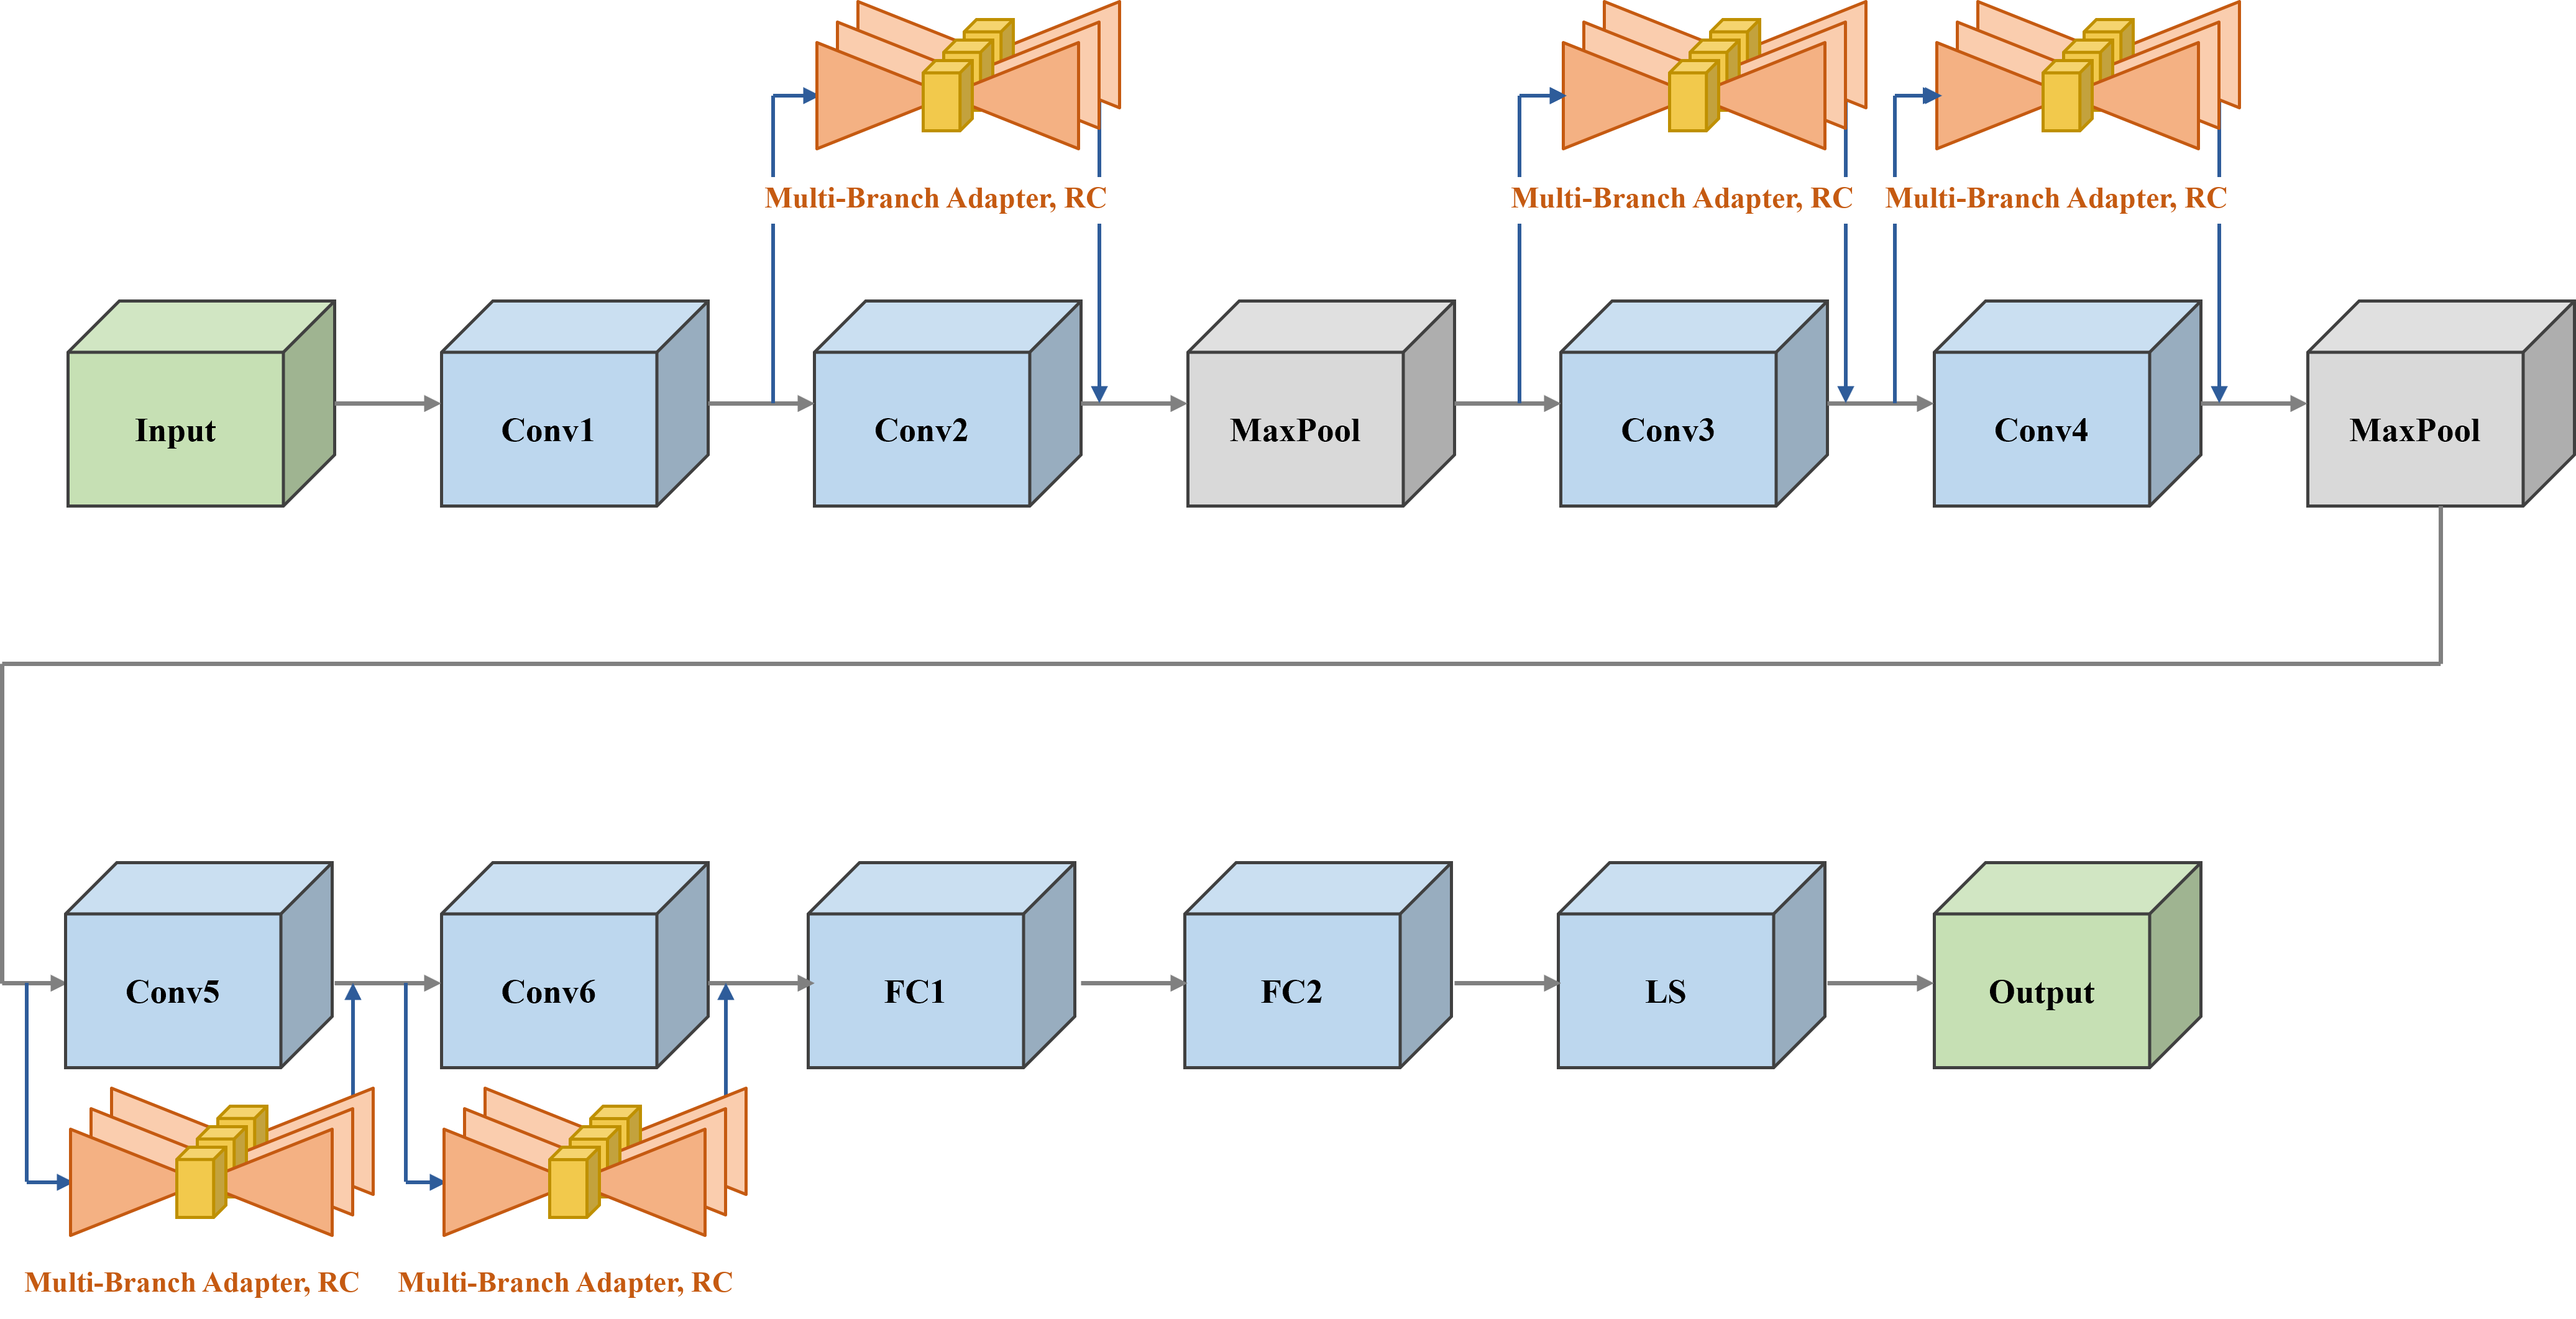
\includegraphics[width=\linewidth,keepaspectratio]{sw_network.png}
\caption{Software Architecture of MARS.}
\label{fig:sw_network}
\end{figure}

\begin{figure}[H]
\centering
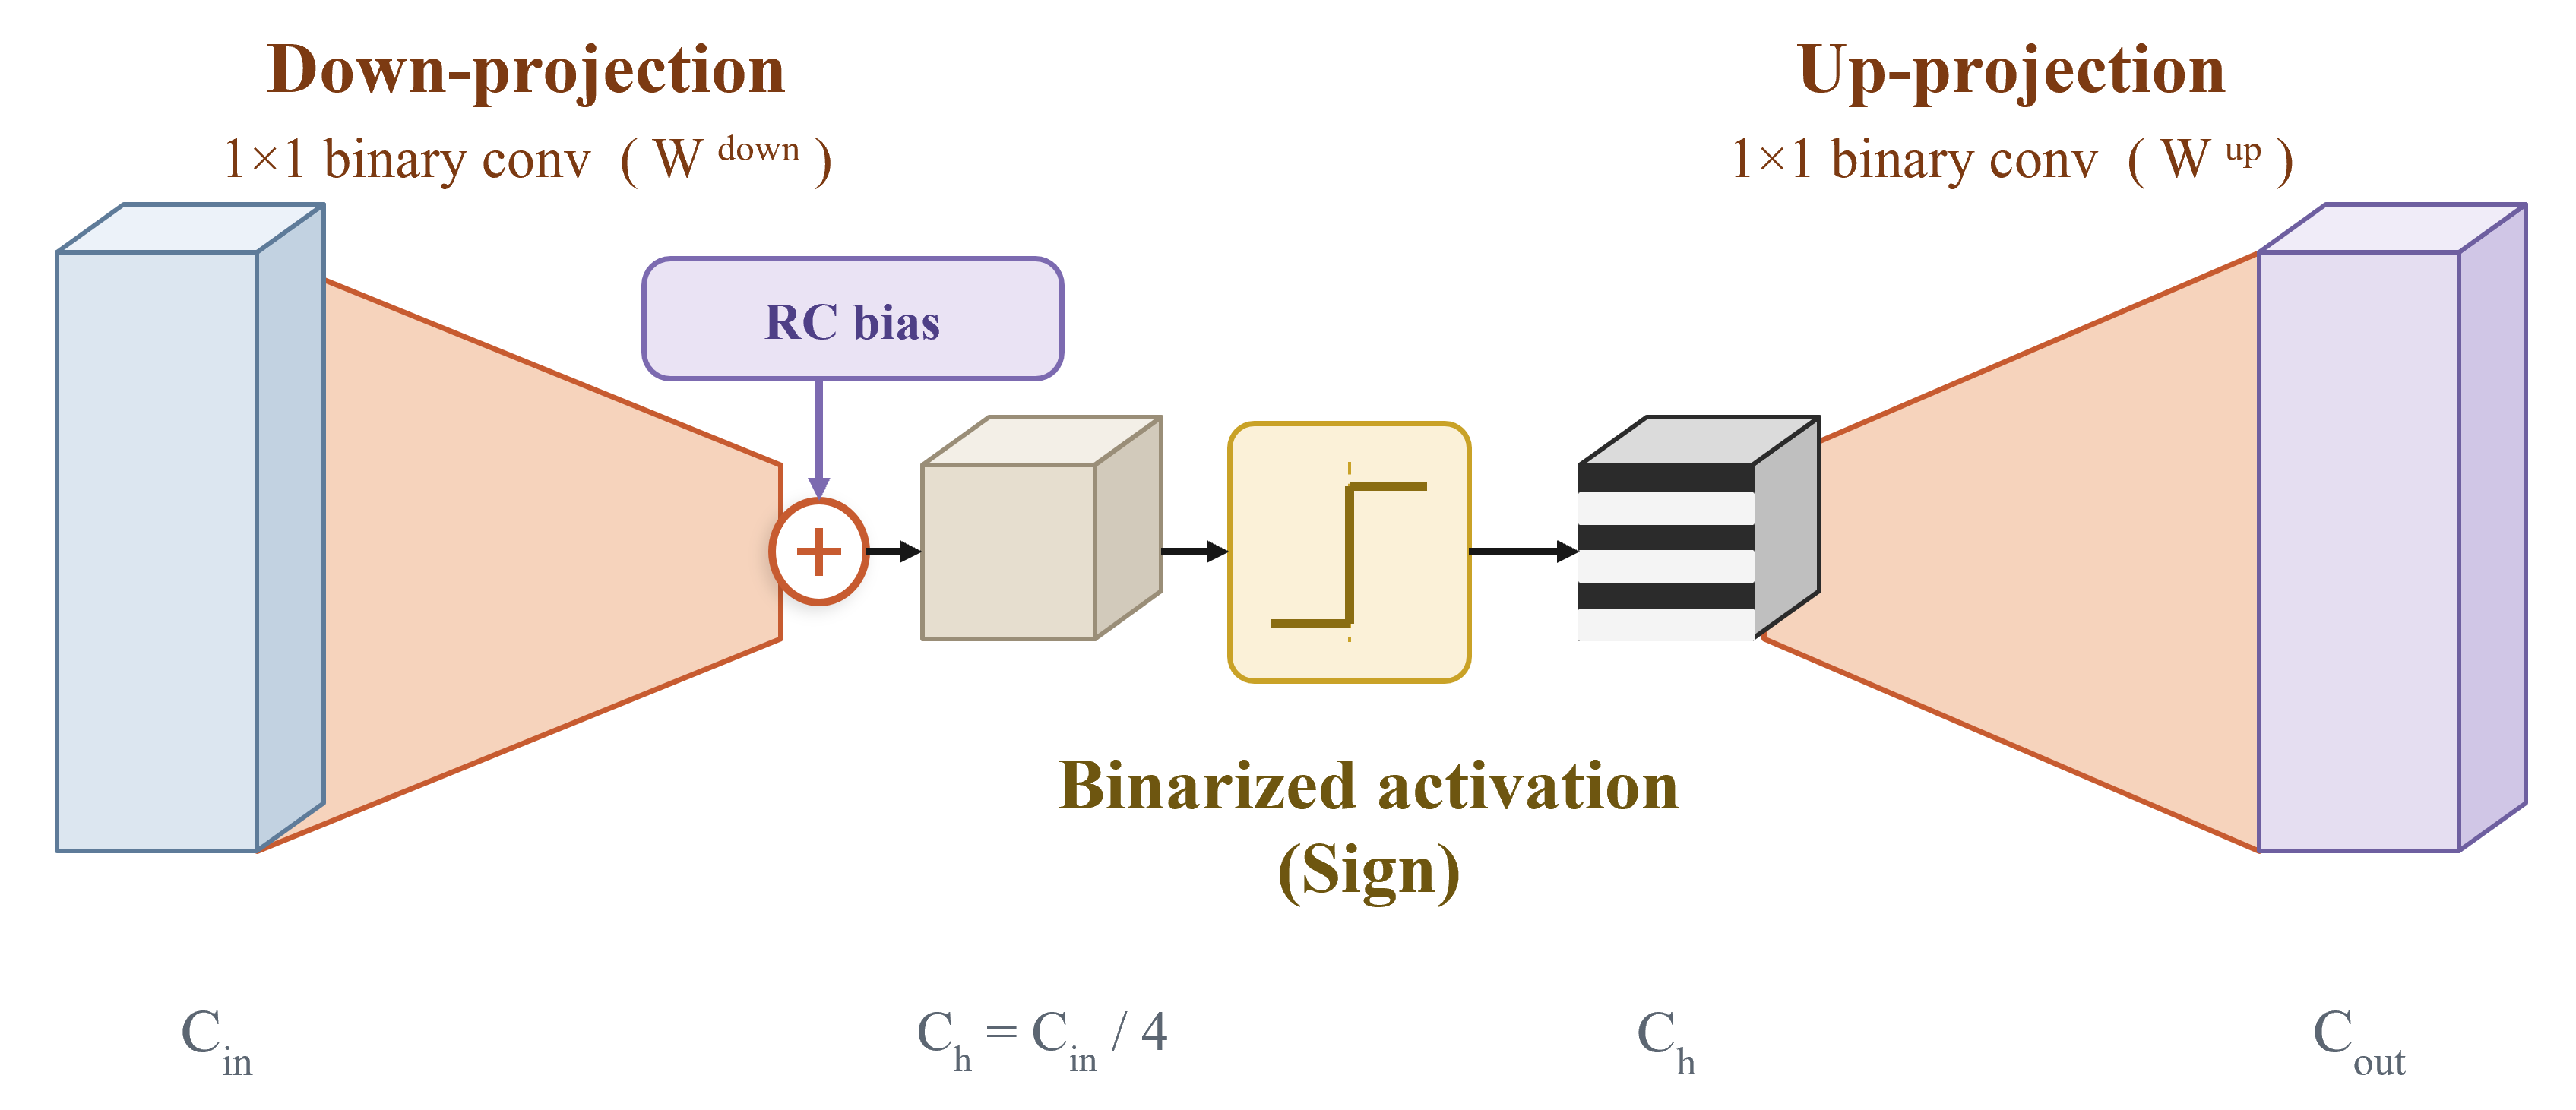
\includegraphics[width=0.85\linewidth,keepaspectratio]{sw_single_adapter.png}
\caption{Conv-Adapter~\cite{Chen2024ConvAdapter} Bottleneck Binarised to 1W1A.}
\label{fig:sw_single_adapter}
\end{figure}

\paragraph{What MARS changes relative to the original Conv-Adapter.}
\label{sec:adapter_vs_convadapter}
The original Conv-Adapter is a full-precision module: its $3\times 3$ depthwise down convolution and $1\times 1$ up-projection are real-valued multiply--accumulate convolutions, its nonlinearity is a real-valued ReLU, and its output is scaled by a learned floating-point factor $\alpha$. None of these operations can be placed on an ultra-low-bit streaming datapath without dedicated multipliers and activation logic. MARS therefore changes each operation at the algorithm level:
\begin{itemize}
    \item \textbf{Spatial operator: $3\times 3$ depthwise down convolution $\to$ $1\times 1$.} In the FPGA-deployed geometry the down convolution is reduced from the original $3\times 3$ depthwise kernel to a $1\times 1$ pointwise projection, eliminating the neighbouring-pixel line buffers entirely; the wide software geometry retains the $3\times 3$ kernel, and the accuracy trade-off of this reduction is quantified in Section~\ref{sec:sw_hw_gap} (Tables~\ref{tab:hw_design_choices} and~\ref{tab:sw_hw_version}).
    \item \textbf{Projections: real multiply--accumulate $\to$ XNOR-popcount.} Under 1-bit weights and 1-bit activations both operands take values in $\{-1,+1\}$, so each multiplication degenerates to a bitwise XNOR and the accumulation to a popcount (Eq.~\ref{eq:down_proj} and~\ref{eq:up_proj})---the same binary inner-product primitive used throughout the 1W1A backbone.
    \item \textbf{Nonlinearity: ReLU $\to$ binary sign.} The real-valued ReLU is replaced by the binary sign function (Eq.~\ref{eq:binary_act}), which emits a single bit per hidden channel. It is precisely this substitution that makes the hidden representation 1-bit and keeps the entire adapter path binary.
    \item \textbf{The bias becomes a first-class, analysed term (RC).} Replacing ReLU by the binary sign discards the per-channel additive shift that ReLU's bias used to provide. MARS isolates this bias as \emph{Residual Correction} (Section~\ref{sec:rc}) and---unlike the original Conv-Adapter, which left the bias active without isolating it as a separate term---shows that its measured effect is substantially larger at 1W1A than at 2--8 bits.
\end{itemize}
The result preserves the down-projection $\to$ binary activation $\to$ up-projection bottleneck topology while changing the spatial operator and arithmetic for hardware compatibility, yielding a fully binary datapath plus a small Int8 correction term; the learned per-branch scale $\alpha$ is retained from Conv-Adapter. The two accuracy mechanisms that this re-design relies on---multi-branch scaling (Section~\ref{sec:multi_adapter}) and RC (Section~\ref{sec:rc})---are analysed in the following sections, while the mapping of these operations onto streaming hardware (including the accumulator-reset realisation of RC and the lookup table that absorbs $\alpha$) is deferred to Chapter~\ref{ch:hardware}. The remainder of this section formalises the three binary operations.

Given an input feature map with $C_{\text{in}}$ channels, the adapter performs three sequential operations:

\paragraph{Down-Projection.} The input activation is projected from $C_{\text{in}}$ channels to a reduced hidden dimension $C_h$, computed as:
\begin{equation}
C_h = \left\lfloor \frac{C_{\text{in}}}{r} \right\rfloor,
\label{eq:hidden_dim}
\end{equation}
where $r$ denotes the reduction ratio, set to $r = 4$ in all MARS configurations. For each hidden unit $j$, the down-projection forms a binary inner product between the down weights and the input over the $C_{\text{in}}$ input channels, initialised by the RC bias:
\begin{equation}
h_j = b_j + \sum_{i=1}^{C_{\text{in}}} \operatorname{XNOR}\bigl(W^{\text{down}}_{j,i}, x_i\bigr), \qquad j = 1, \ldots, C_h.
\label{eq:down_proj}
\end{equation}

Each symbol is defined as follows:
\begin{itemize}
    \item $h_j$: the hidden accumulator value for hidden channel $j$ (16-bit signed register).
    \item $b_j$: the exported hardware-domain 8-bit signed (Int8) RC bias for channel $j$ (Section~\ref{sec:rc}), sign-extended to the 16-bit accumulator width and loaded as the accumulator initial value before any accumulation begins; this exported value already absorbs the binary inner-product offset described below and is not the raw floating-point training bias.
    \item $W^{\text{down}}_{j,i} \in \{0,1\}$: the binary down-projection weight from input channel $i$ to hidden channel $j$, stored in distributed RAM (\texttt{ram\_down}).
    \item $x_i \in \{0,1\}$: the binary input activation on channel $i$.
    \item $\operatorname{XNOR}(\cdot,\cdot)$: the bitwise XNOR operator (1 when the two bits match); the sum $\sum_i \operatorname{XNOR}(W^{\text{down}}_{j,i}, x_i)$ is the XNOR-popcount binary inner product, realised in hardware as XNOR followed by popcount over SIMD-width chunks (Chapter~\ref{ch:hardware}).
    \item $C_{\text{in}}, C_h$: the input and hidden channel counts.
\end{itemize}

The XNOR-popcount primitive is a standard binary neural network operation \cite{Rastegari2016XNOR, Hubara2016BinarizedNN}. MARS's design choice lies in how this primitive is organized: the accumulator is initialized with the RC bias $b_j$ rather than zero, enabling mixed-precision correction without additional hardware (Section~\ref{sec:rc}). \emph{Encoding convention:} bits are stored as $\{0,1\}$; under the $\{0,1\}\!\leftrightarrow\!\{-1,+1\}$ map the $\{-1,+1\}$ inner product equals $2\cdot\text{popcount}-N$, and the constant $-N$ offset is folded into the per-channel bias/threshold, so the raw XNOR-popcount count is used directly above.

\paragraph{Binary Activation.} The hidden representation is binarised via sign extraction:
\begin{equation}
a_j = \begin{cases} 1 & h_j \geq 0, \\ 0 & \text{otherwise,} \end{cases} \qquad \mathbf{a} = (a_1, \ldots, a_{C_h}).
\label{eq:binary_act}
\end{equation}
This operation requires only the MSB of each hidden accumulator, avoiding dedicated comparator logic.

\paragraph{Up-Projection.} The binarised hidden vector $\mathbf{a} \in \{0,1\}^{C_h}$ is projected back to the $C_{\text{out}}$ output channels. For each output channel $o$, the output value is the binary inner product of the up weights and the hidden vector:
\begin{equation}
z_o = \sum_{j=1}^{C_h} \operatorname{XNOR}\bigl(W^{\text{up}}_{o,j}, a_j\bigr), \qquad o = 1, \ldots, C_{\text{out}},
\label{eq:up_proj}
\end{equation}
where:
\begin{itemize}
    \item $z_o$: the output value for channel $o$ (8-bit unsigned popcount).
    \item $a_j \in \{0,1\}$: the binarised hidden activation on channel $j$.
    \item $W^{\text{up}}_{o,j} \in \{0,1\}$: the binary up-projection weight from hidden channel $j$ to output channel $o$, stored in distributed RAM (\texttt{ram\_up}).
    \item $C_h, C_{\text{out}}$: the hidden and output channel counts.
\end{itemize}

In hardware the output channels are produced $P$ at a time (PE-parallel), packing the corresponding $P$ weight vectors into a single wide RAM word per output step; the full PE/SIMD mapping is given in Chapter~\ref{ch:hardware}.

\paragraph{Spatial Center Selection.} For the backbone's $3 \times 3$ convolutional layers, the adapter operates on the center pixel of each $3 \times 3$ sliding window rather than all nine positions---this is precisely how the adapter's $1 \times 1$ down convolution is realised on the backbone's streamed window. Since the FINN MVAU streams the nine kernel positions of the backbone window sequentially (one input chunk per cycle), the adapter only needs to process the center position (position 4 of 0--8), reducing the adapter computational load by $9\times$. The center pixel is identified by a cycle counter:
\begin{equation}
\text{center active} \iff 4K \leq \texttt{cycle\_cnt} < 5K,
\end{equation}
where $K = C_{\text{in}} / S$ is the number of chunks per kernel position. The adapter FSM gates the accumulation accordingly, producing valid output only after the center pixel chunks have been processed.

Table~\ref{tab:adapter_config} lists the adapter configuration for each convolutional layer.

\begin{table}[H]
\centering
\caption{Adapter Bottleneck Configuration per Layer}
\label{tab:adapter_config}
\begin{tabular}{ccccc}
\toprule
\textbf{Layer} & \textbf{$C_{\text{in}}$} & \textbf{$C_{\text{out}}$} & \textbf{$R$} & \textbf{$C_h$} \\
\midrule
Conv1 (MVAU0) & 3   & 64  & -- & --  \\
Conv2 (Super1) & 64  & 64  & 4  & 16  \\
Conv3 (Super2) & 64  & 128 & 4  & 16  \\
Conv4 (Super3) & 128 & 128 & 4  & 32  \\
Conv5 (Super4) & 128 & 256 & 4  & 32  \\
Conv6 (Super5) & 256 & 256 & 4  & 64  \\
\bottomrule
\end{tabular}
\begin{flushleft}
\footnotesize Conv1 is excluded from adapter insertion as it performs generic low-level feature extraction \cite{Chen2024ConvAdapter}.
\end{flushleft}
\end{table}

The complete adapter forward computation is summarised in Algorithm~\ref{alg:adapter_forward}.

\begin{algorithm}[htbp]
\caption{Binary Adapter Forward Computation}
\label{alg:adapter_forward}
\small
\begin{algorithmic}[1]
\Require Input stream $\mathbf{x}^{(k)}$ for $k = 0, \ldots, K-1$; weights $\mathbf{W}_{\text{down}}, \mathbf{W}_{\text{up}}$; RC bias $\mathbf{b}_{\text{RC}}$
\Ensure Output popcount vector $\mathbf{o}$ of dimension $P$ per output step
\State \textbf{// Phase 1: Down-Projection (iterate over input chunks)}
\For{$j = 0$ to $C_h - 1$}
    \State $h_j \gets b_{\text{RC}}^{(j)}$ \Comment{Initialize with RC bias}
\EndFor
\For{$k = 0$ to $K - 1$} \Comment{Only center pixel chunks}
    \For{$j = 0$ to $C_h - 1$}
        \State $h_j \gets h_j + \text{popcount}(\text{XNOR}(\mathbf{w}_{\text{down}}^{(j,k)}, \mathbf{x}^{(k)}))$
    \EndFor
\EndFor
\State \textbf{// Phase 2: Binary Activation}
\For{$j = 0$ to $C_h - 1$}
    \State $a_j \gets \mathbf{1}[h_j \geq 0]$ \Comment{Sign extraction}
\EndFor
\State \textbf{// Phase 3: Up-Projection (iterate over output steps)}
\For{$s = 0$ to $C_{\text{out}}/P - 1$}
    \For{$p = 0$ to $P - 1$}
        \State $o_p \gets \text{popcount}(\text{XNOR}(\mathbf{a}, \mathbf{w}_{\text{up}}^{(s,p)}))$
    \EndFor
    \State \textbf{emit} $(o_0, o_1, \ldots, o_{P-1})$
\EndFor
\end{algorithmic}
\end{algorithm}

The single-adapter parameter overhead is:
\begin{equation}
\Delta P = \sum_{l=1}^{5} \bigl( C_{\text{in}}^{(l)} \cdot C_h^{(l)} + C_h^{(l)} \cdot C_{\text{out}}^{(l)} + C_h^{(l)} + 1 \bigr) = 58{,}533,
\end{equation}
where the per-layer terms are the down-projection ($C_{\text{in}}^{(l)} C_h^{(l)}$), the up-projection ($C_h^{(l)} C_{\text{out}}^{(l)}$), the Int8 RC bias ($C_h^{(l)}$), and the scalar $\alpha$ ($+1$). This represents $\Delta P / P_{\text{backbone}} = 58{,}533 / 1{,}546{,}690 \approx 3.78\%$ of the backbone parameters.

\section{Residual Correction (RC) and the 1-Bit Empirical Finding}\footnote{Throughout this thesis ``Residual Correction (RC)'' refers specifically to the Int8-quantised bias on the down-convolution of an adapter, exported as the per-layer artefact \texttt{adapter\_\{l\}\_rc.dat} and absorbed at runtime into the adapter accumulator reset (Section~\ref{sec:rc}). This is distinct from the more common ``residual connection'' (i.e., a skip-link in ResNet-style architectures); we use the term ``Correction'' to emphasise its corrective role at 1-bit while keeping the established abbreviation ``RC''.}
\label{sec:rc}

\subsection{Definition and HW Realization}

We adopt the bottleneck Conv-Adapter structure of Chen et~al.~\cite{Chen2024ConvAdapter} as the base adapter; in the deployed configuration each branch is a $1\times 1$ down convolution followed by a binary activation and a $1\times 1$ up convolution scaled by a learned factor $\alpha$. We term the Int8-quantised bias on the down convolution the \textbf{Residual Correction (RC)}, following the naming used by our hardware export pipeline where it is emitted as a separate FPGA artifact \texttt{adapter\_\{l\}\_rc.dat} (five per-layer files, eight-bit signed). The bias $b_j$ is exactly the additive term of the down-projection accumulator defined in Eq.~(\ref{eq:down_proj}).
At the RTL level RC introduces no additional adder, DSP slice, or pipeline stage: the per-channel Int8 bias is absorbed into the accumulator reset value (Section~\ref{sec:adapter_rtl}), so the correction is realized through control-path multiplexing of an existing register; its distributed-RAM storage (\texttt{ram\_rc}) and accumulator-initialisation control are counted in the adapter overhead.
\begin{equation}
\texttt{hidden\_acc[j]} \xleftarrow{\text{init}} \texttt{ram\_rc[j]}, \quad j = 0, \ldots, C_h - 1.
\end{equation}
The RC values are stored in a small distributed RAM (\texttt{ram\_rc}, $C_h \times 16$~bits) and the initialization is absorbed into the existing reset/window-start control logic.

\subsection{Why RC Matters under 1-Bit Quantisation}

Under 1-bit weight, 1-bit activation (1W1A) the down-convolution output is fed into a binary sign function. Without a learnable additive shift, the sign function reduces to a hard \emph{threshold-at-zero} decision and the adapter loses the ability to relocate this threshold per channel. As soon as the activation is widened to two or more bits, the measured role of RC becomes small (Table~\ref{tab:bitwidth_sweep_svhn}); a plausible explanation is that the additional quantisation levels preserve magnitude information that downstream layers can exploit, though this is a hypothesis rather than a verified mechanism. RC is therefore not a generic enhancement: it is the component that recovers the per-channel shift the 1-bit binary activation removes.

\subsection{Empirical Finding: A Disproportionate Role at 1-Bit}

The effect of RC was previously assumed to be small because the original Conv-Adapter pipeline did not isolate the down-convolution bias as a separate term---the \texttt{bias=True} default of PyTorch \texttt{Conv2d} keeps the bias active, so its 1-bit-specific role was not reported as an independent ablation in that work. We re-implemented the ablation so that \texttt{bias=False, bias\_quant=None} is enforced when RC is disabled and \texttt{bias=True, bias\_quant=Int8Bias} when RC is enabled, with all other adapter dimensions held fixed.

Two findings follow directly from this corrected ablation (full ablation tables in Table~\ref{tab:bitwidth_sweep_svhn} and Sections~\ref{sec:rc_ablation_svhn} and~\ref{sec:rc_cross_dataset}):
\begin{enumerate}
    \item \textbf{1-bit: RC is critical.} On CIFAR-10$\to$SVHN at 1W1A, removing RC drops accuracy by $15$--$17$~percentage points in the wide geometry (Table~\ref{tab:rc_ablation_svhn}) and $20$--$23$~percentage points in the FPGA-deployed geometry (Table~\ref{tab:rc_ablation_hw}), at every multi-branch adapter configuration ($M{=}1$--$4$). The mechanism aligns with the binary-sign argument above.
    \item \textbf{$\geq$2-bit: RC has a substantially smaller measured effect.} For backbone activation widths of 2, 4, and 8 bits, removing RC changes accuracy by at most 1.4 percentage points---and typically under 0.3---on the same source--target pair (Table~\ref{tab:bitwidth_sweep_svhn}).
\end{enumerate}

In view of these results the role of RC in this work is reframed: it is not a generic accuracy improvement but a corrective term with a substantially larger measured effect at 1W1A, and---because it adds no arithmetic or datapath cost---it is committed unconditionally in the deployed bitstream.

\section{Multi-Branch Adapter Scaling}
\label{sec:multi_adapter}

\subsection{Architecture}

Multi-Branch Adapter scaling is the mechanism through which this thesis raises transfer accuracy above the Conv-Adapter single-branch baseline~\cite{Chen2024ConvAdapter} under ultra-low-bit quantisation. It employs $M$ parallel adapter branches within each layer, directly targeting the degradation of the single-branch adapter contribution that we observe specifically at 1-bit (Table~\ref{tab:bitwidth_sweep_svhn}). Each branch has independent weights and RC biases. For each output channel $o$, the $M$ branch outputs are merged by learned scaling factors:
\begin{equation}
y_o = \sum_{i=1}^{M} \alpha_i\, z_o^{(i)}, \qquad o = 1, \ldots, C_{\text{out}},
\label{eq:multi_adapter}
\end{equation}
where:
\begin{itemize}
    \item $y_o$: the merged multi-branch adapter output for channel $o$.
    \item $M$: the number of parallel adapter branches ($M{=}1$ through $M{=}4$).
    \item $\alpha_i$: a learnable scaling factor for the $i$-th branch, trained jointly during fine-tuning. At deployment, $\alpha_i$ is quantised and absorbed into the contribution LUT.
    \item $z_o^{(i)}$: the output of the $i$-th branch on channel $o$, computed by the down-projection, binary activation, and up-projection pipeline of Section~\ref{sec:adapter_arch}.
\end{itemize}

\paragraph{Training.}
All task-dependent parameters---the $M$ branches and the classifier---are trained jointly, end-to-end, with the backbone frozen. Each branch's down- and up-projection weights are binarised in the forward pass,
\begin{equation}
W^{\text{down},(i)} = \operatorname{sign}\bigl(\widetilde{W}^{\text{down},(i)}\bigr), \qquad
W^{\text{up},(i)} = \operatorname{sign}\bigl(\widetilde{W}^{\text{up},(i)}\bigr),
\label{eq:binarise}
\end{equation}
and the backward pass uses the straight-through estimator
\begin{equation}
\frac{\partial \operatorname{sign}(u)}{\partial u} \;\approx\; \mathbf{1}_{|u| \le 1},
\label{eq:ste}
\end{equation}
so ADAM updates the real-valued latent weights $\widetilde{W}$ and the real-valued down-convolution bias $b^{(i)}$ (the RC term). The per-branch scale $\alpha_i$ multiplies its branch output linearly, so it receives the exact gradient
\begin{equation}
\frac{\partial L}{\partial \alpha_i} \;=\; \Bigl\langle \frac{\partial L}{\partial y},\; z^{(i)} \Bigr\rangle,
\label{eq:alpha_grad}
\end{equation}
with no estimator involved. Nothing in the formulation forces the branches apart: they share the same structure and diverge only through independent random initialisation and joint training. At export, $\alpha_i$ is quantised into the Q8 contribution LUT and $b^{(i)}$ is folded into the accumulator initial value (Section~\ref{sec:rc}).

\begin{figure}[H]
\centering
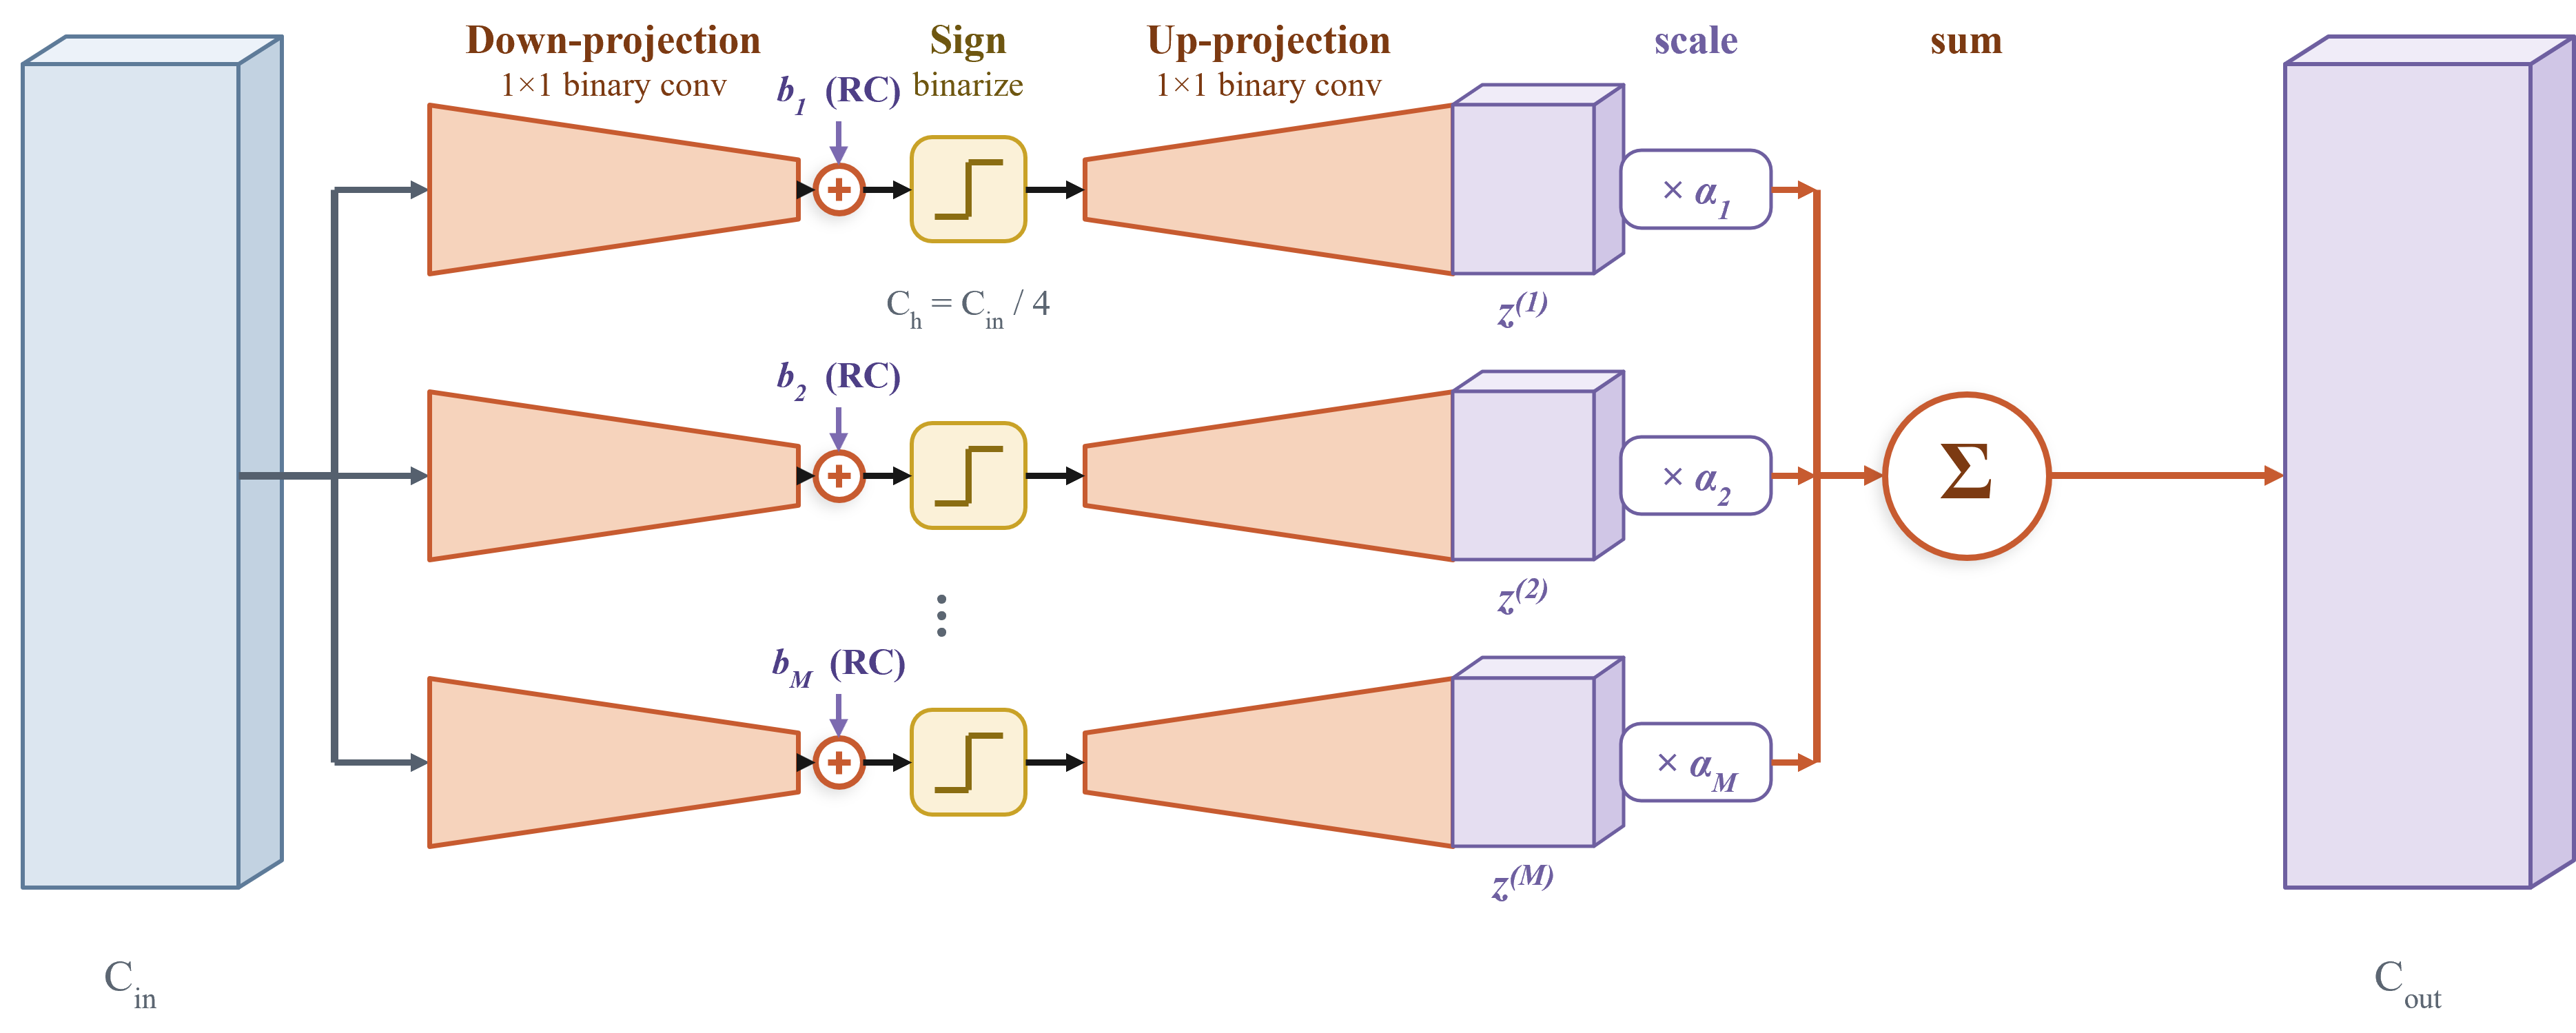
\includegraphics[width=\linewidth,keepaspectratio]{sw_multiadapter.png}
\caption[Multi-Branch Adapter: $M$ Parallel Binary Branches]{Multi-Branch Adapter: $M$ Parallel Binary Branches Summed Before Thresholding.}
\label{fig:sw_multiadapter}
\end{figure}

The total parameter overhead scales linearly with $M$:
\begin{equation}
\Delta P(M) = M \times 58{,}533,
\end{equation}
yielding $\Delta P / P_{\text{backbone}} \approx 3.78\% \times M$. The configurations m1 through m4 correspond to $M \in \{1, 2, 3, 4\}$. The measured parameter and post-synthesis hardware cost at each $M$ is quantified in Table~\ref{tab:mb_cost}.

\subsection{Theoretical Computational Cost}

The computational cost of the backbone and adapter branches is analyzed as follows. The backbone consists of six $3 \times 3$ convolutional layers and three fully connected layers:

\begin{table}[H]
\centering
\caption{Backbone Computational Cost Breakdown (CIFAR-10, $32 \times 32 \times 3$ Input)}
\label{tab:backbone_macs}
\begin{tabular}{lrrr}
\toprule
\textbf{Layer} & \textbf{Output Shape} & \textbf{MACs} \\
\midrule
Conv1 & $30 \times 30 \times 64$  & 1{,}555{,}200 \\
Conv2 & $28 \times 28 \times 64$  & 28{,}901{,}376 \\
Conv3 & $12 \times 12 \times 128$ & 10{,}616{,}832 \\
Conv4 & $10 \times 10 \times 128$ & 14{,}745{,}600 \\
Conv5 & $3 \times 3 \times 256$   & 2{,}654{,}208 \\
Conv6 & $1 \times 1 \times 256$   & 589{,}824 \\
FC1--FC3 & $512, 512, 10$          & 398{,}336 \\
\midrule
\textbf{Total} & & \textbf{59.46 M MACs} \\
\bottomrule
\end{tabular}
\end{table}

Each adapter branch employs $1 \times 1$ down- and up-projections across five layers. Two operation counts must be distinguished. The \emph{software reference} implementation computes both projections over the full input feature map of each host layer and then crops the border to align with the convolution output (compute-then-crop), executing $4{,}227{,}072 \approx 4.23$~M MACs per branch; this count also serves as the per-branch adapter term in the cross-platform normalisation of Section~\ref{sec:cross_platform}. The \emph{deployed RTL} evaluates the projections only at the output positions through its centre-selection logic (Chapter~\ref{ch:hardware}), executing $3{,}010{,}560 \approx 3.01$~M MACs per branch. The unified \emph{model-level} formula, used consistently for cross-platform accounting, is:
\begin{equation}
\text{OPs}_{\text{total}} = 2 \times \bigl(59.46 + 4.23 \times M\bigr) \text{ MOPs/image},
\end{equation}
where we define $1 \text{ MAC} = 2 \text{ OPs}$. For $M = 1$, the total is 127.38~MOPs/image.

\subsection{Accuracy Recovery Through Branch Scaling}
\enlargethispage{2\baselineskip}

Multi-Branch Adapter scaling aims to progressively recover the accuracy lost to ultra-low-bit quantisation of the adapter: increasing $M$ lets each branch learn a different correction subspace at the linear resource cost derived above. Increasing $M$ is expected to improve mean transfer accuracy with diminishing average returns---the shared bottleneck dimension bounds the total information capacity regardless of additional branches---although individual transfer trajectories need not be monotonic under optimisation variance. The branch sweeps quantifying this recovery over all twenty backbone--target pairs and both geometries are reported in Chapter~\ref{ch:experiments} (Sections~\ref{sec:v6_multi_adapter} and~\ref{sec:sw_hw_gap}).

% ==========================================================
% References
% ==========================================================

\chapter{MARS NPU Architecture Design}
\label{ch:hardware}

This chapter describes the RTL-level hardware design of the MARS accelerator. Section~\ref{sec:sys_arch} presents the system-level architecture. Section~\ref{sec:super_wrapper} details the Super Wrapper that integrates the Adapter IP into the MVAU. Section~\ref{sec:adapter_rtl} describes the Adapter IP internal pipeline. Section~\ref{sec:adder_thresh} explains the Stream Adder + Threshold module.

\section{System Architecture Overview}
\label{sec:sys_arch}

The MARS accelerator targets an SoC FPGA that integrates a micro-processor subsystem with programmable logic (PL). The system operates at 100~MHz. The specific device and development board used for the experiments are stated in Chapter~\ref{ch:experiments}.

Figure~\ref{fig:system_arch} shows the top-level architecture. The micro-processor subsystem handles system control, data movement, and inference-flow management via off-chip memory. The PL implements the streaming dataflow inference pipeline, comprising:
\begin{itemize}
    \item \textbf{Input/Output DMA}: streaming interfaces for data transfer between the micro-processor subsystem and the PL.
    \item \textbf{MVAU0}: Unmodified FINN-generated MVAU for the first convolutional layer (Conv1).
    \item \textbf{Super1--Super5}: Five adapter-enhanced MVAU modules with custom RTL, hosting the Conv2--Conv6 layers.
    \item \textbf{MVAU6--MVAU8}: FINN-generated fully connected layers (FC1--FC3; MVAU8 is the classifier).
    \item \textbf{MaxPool $\times$ 2}: Pooling modules between convolutional stages.
    \item \textbf{LabelSelect}: Final classification output.
\end{itemize}

\begin{figure}[H]
\centering
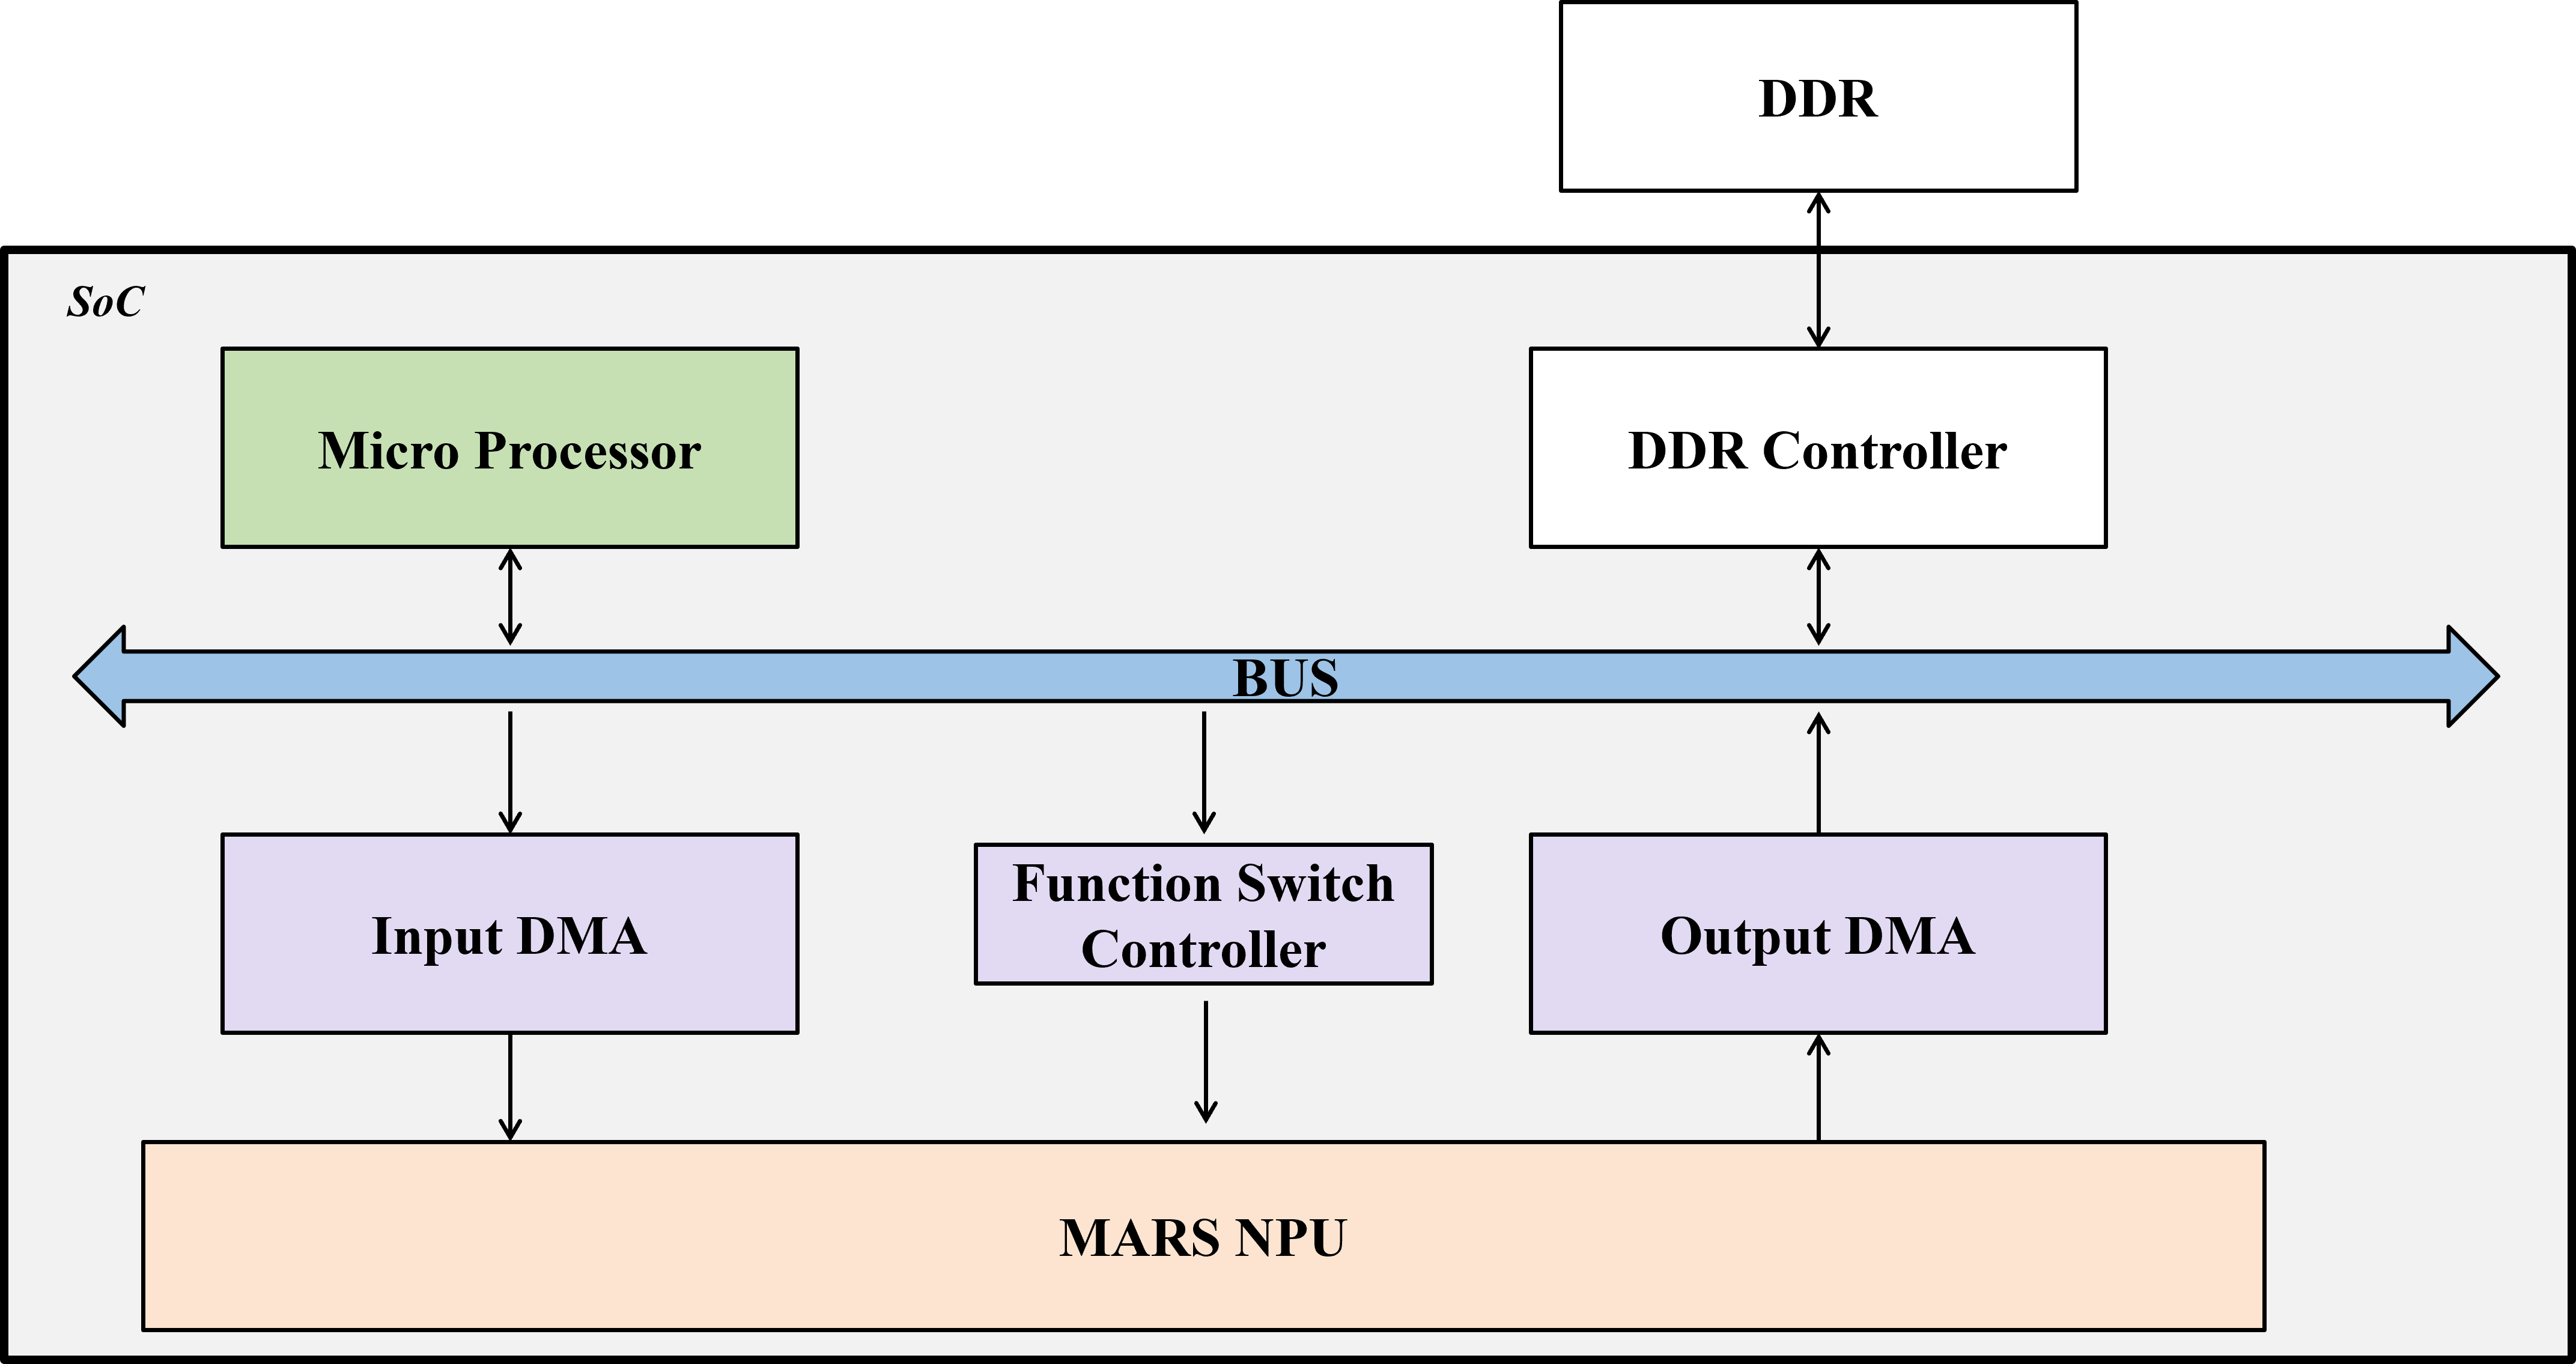
\includegraphics[width=\linewidth,keepaspectratio]{fig42_mars_soc.png}
\caption{MARS Accelerator System Top-Level Architecture.}
\label{fig:system_arch}
\end{figure}

For reference, Figure~\ref{fig:mvau_baseline_pipeline} shows the unmodified streaming pipeline that FINN generates for the same 1W1A VGG-like backbone. Each of Conv1--Conv6 is realised by a single FINN MVAU module connected in series; this is the pipeline upon which the Adapter Super Wrapper in Section~\ref{sec:super_wrapper} is built.

\begin{figure}[H]
\centering
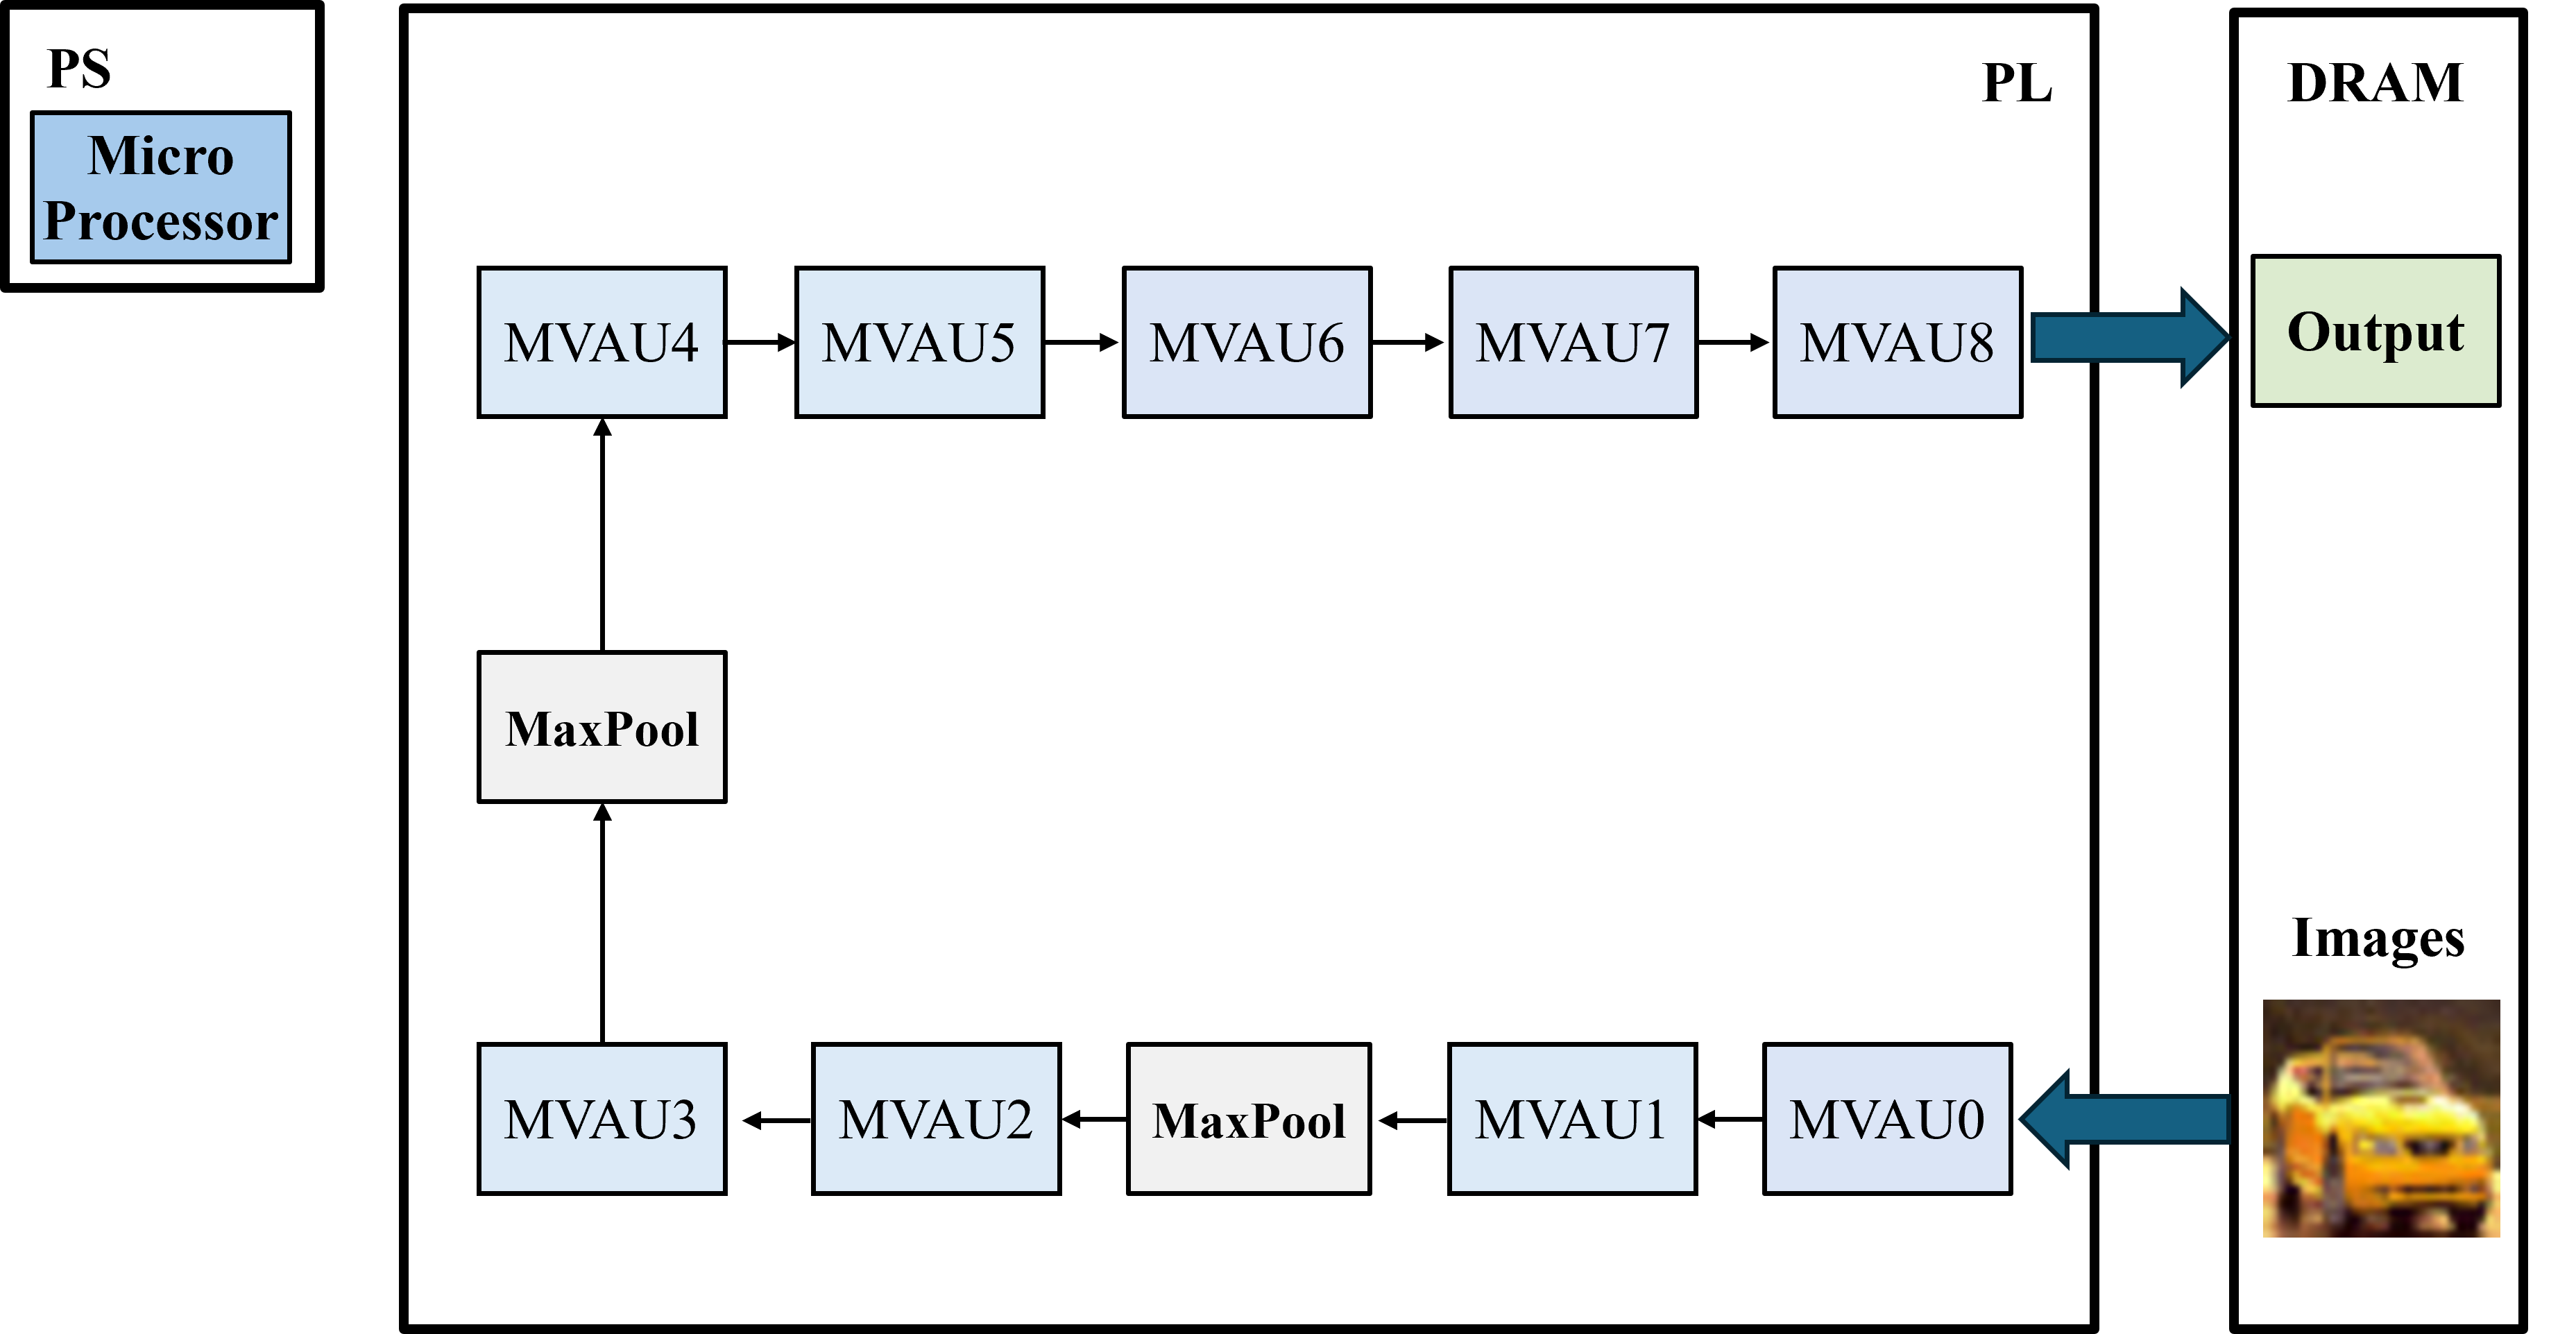
\includegraphics[width=\linewidth,keepaspectratio]{hw_finn_singletask_npu.png}
\caption{Baseline FINN Streaming Inference Pipeline (No Adapter).}
\label{fig:mvau_baseline_pipeline}
\end{figure}

The streaming dataflow pipeline is organized as a two-row layout: the first row contains Input DMA $\to$ MVAU0 $\to$ Super1--Super3 $\to$ MaxPool; the second row continues with Super4--Super5 $\to$ MVAU6--MVAU8 $\to$ Output DMA. All inter-module connections use streaming protocol.

Figure~\ref{fig:finn_rtl_flow} provides a detailed view of the complete pipeline, distinguishing FINN-generated modules (blue) from custom Adapter-Enhanced Super Wrappers (orange), and includes an expanded view of the Super Wrapper internal structure.

\begin{figure}[H]
\centering
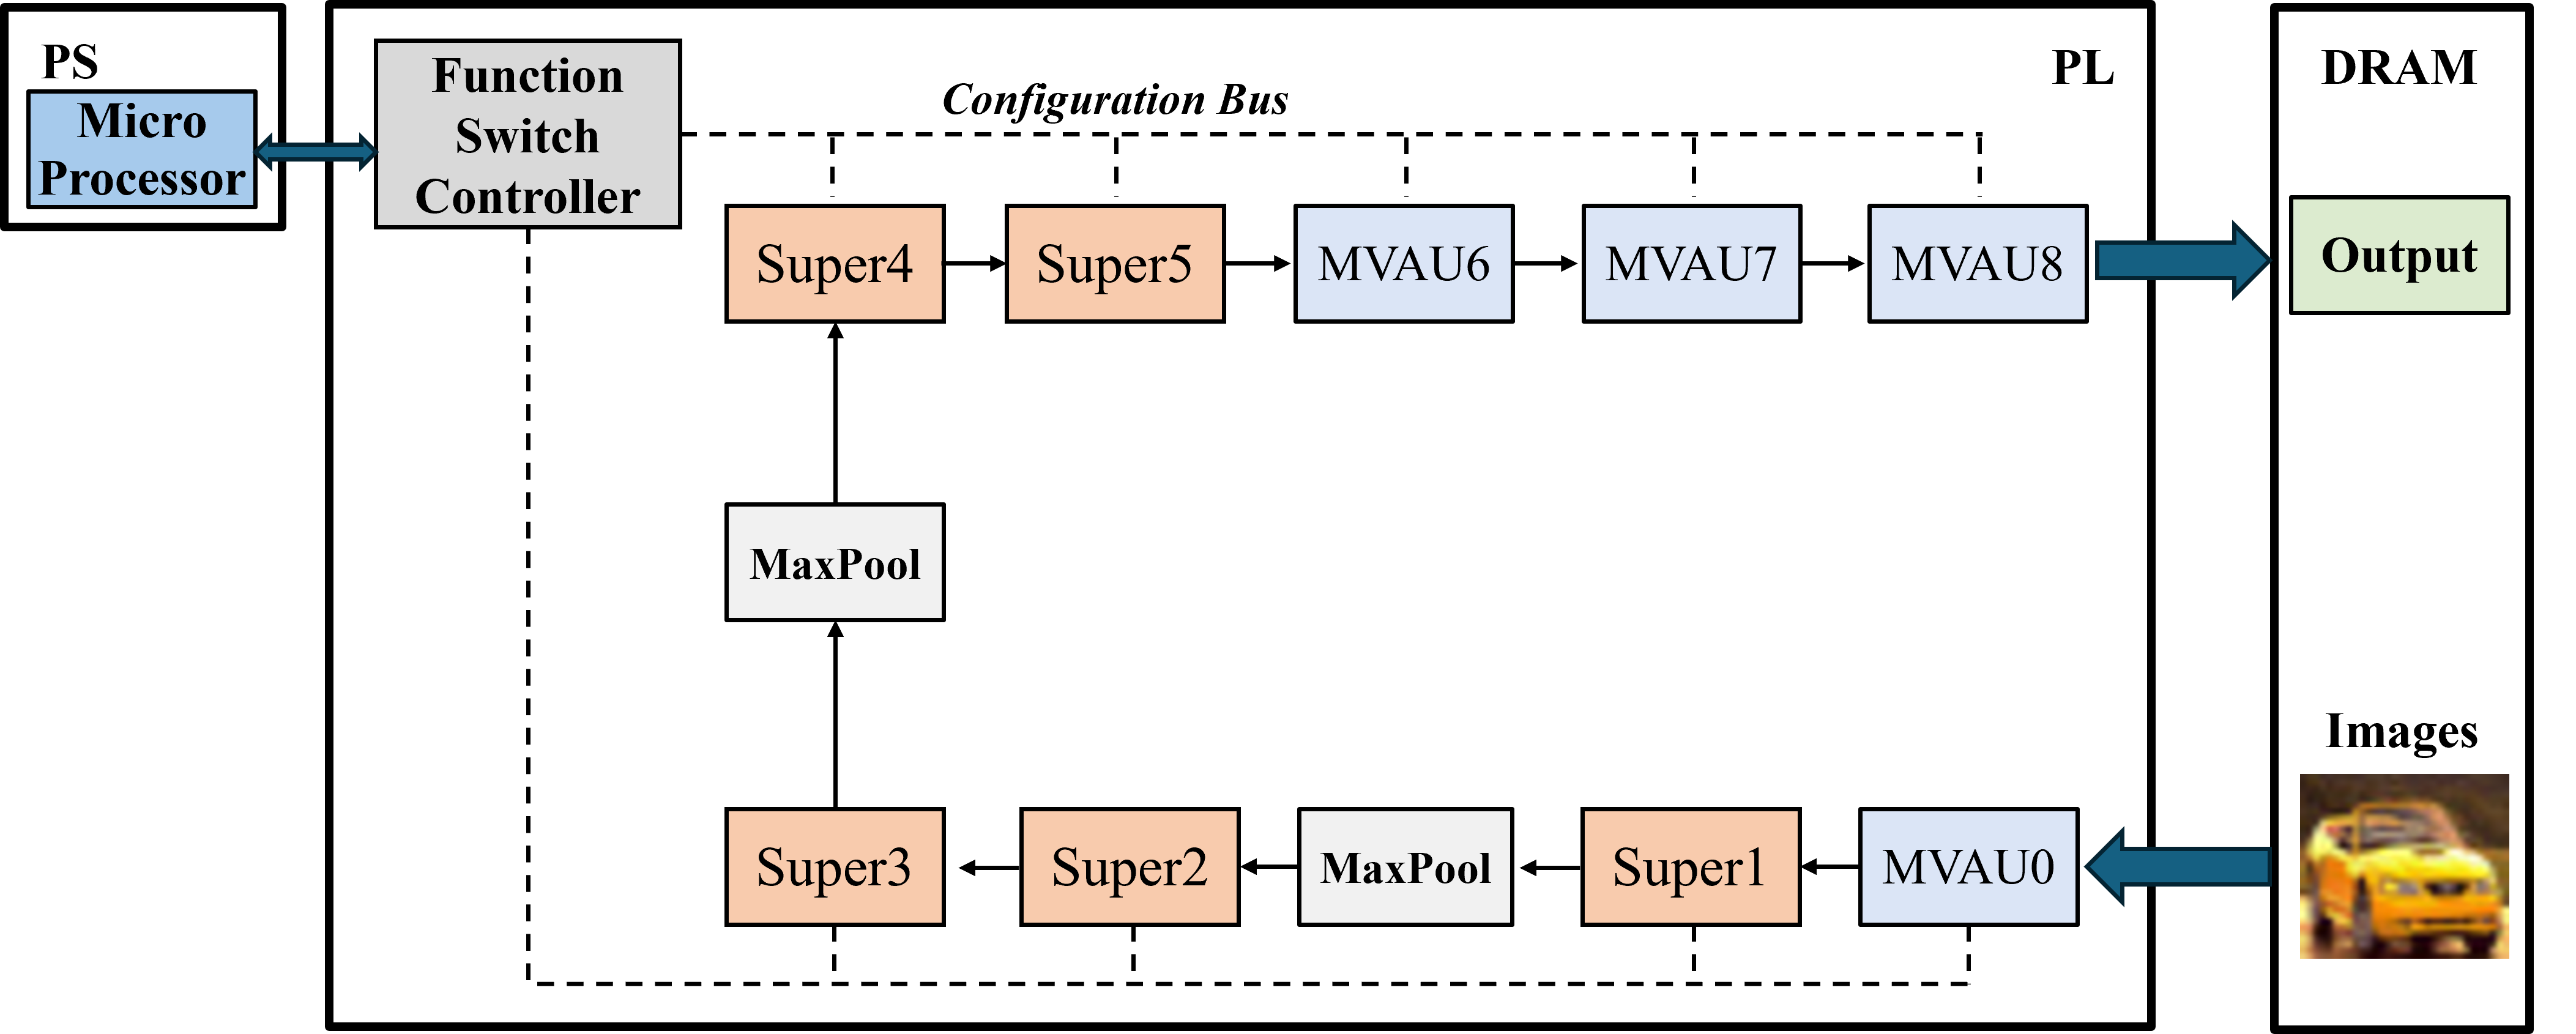
\includegraphics[width=\linewidth,keepaspectratio]{fig44_mars_arch.png}
\caption{MARS Streaming Dataflow Pipeline.}
\label{fig:finn_rtl_flow}
\end{figure}

\paragraph{Module provenance: hand-crafted RTL vs FINN-generated.}
\label{sec:module_provenance}

MARS combines two source streams in the deployed bitstream: backbone-class modules generated by the FINN dataflow compiler (Section~\ref{sec:related_finn}) and the integration/runtime-switching logic that is hand-crafted RTL specific to this thesis. Table~\ref{tab:module_provenance} lists the provenance of every module in the streaming dataflow partition so that readers can map each block in the system diagrams of this chapter to its origin and find the corresponding source file.

\begin{table}[H]
\centering
\caption{Provenance of Each Module in the Deployed MARS Dataflow.}
\label{tab:module_provenance}
\scriptsize
\renewcommand{\arraystretch}{0.95}%
\begin{tabularx}{\textwidth}{@{}ll>{\raggedright\arraybackslash}X@{}}
\toprule
\textbf{Module} & \textbf{Origin} & \textbf{Role} \\
\midrule
MVAU\_hls\_0/6/7/8 & FINN-generated & MVAU0 (first convolution) and MVAU6/7/8 (fully connected + classifier) matrix-vector-activation units; no adapter attached \\
ConvolutionInputGenerator\_rtl\_0..5 & FINN-generated & Sliding-window image patch generators \\
StreamingDataWidthConverter\_rtl\_0..9 & FINN-generated & Stream width adapters \\
StreamingFIFO\_rtl\_0..6 & FINN-generated & Backbone inter-stage FIFOs \\
StreamingMaxPool\_hls\_0..1 & FINN-generated & Backbone max-pool layers \\
Thresholding\_rtl\_0 & FINN-generated & Backbone threshold unit \\
LabelSelect\_hls\_0 & FINN-generated & Final label arg-max \\
IODMA\_hls\_0 & FINN-generated & Input/output DMA \\
\midrule
MVAU\_hls\_1..5 & FINN-generated, hand-modified & MVAU cores wrapped into Super1--5 to host an adapter (Conv2--Conv6 layers); the in-module threshold is decoupled and the raw 32-bit partial sum is exposed on the output stream so the adapter contribution can be fused before binarisation \\
\midrule
Adapter\_MVAU\{1..5\}.v & Hand-crafted RTL & Adapter datapath (down/up/RC/popcount/XNOR) \\
Stream\_Adder\_Threshold\_mvau\{1..5\}.v & Hand-crafted RTL & Adapter contribution fusion + Q8 threshold \\
Simple\_FIFO\_mvau\{1..5\}.v & Hand-crafted RTL & Per-adapter synchronisation FIFO (depth 64) \\
Stream\_Splitter\_mvau\{1..5\}.v & Hand-crafted RTL & Backbone/adapter stream split \\
MVAU\{1..5\}\_Super\_Wrapper.v & Hand-crafted RTL & Per-layer Super Wrapper integrating the modified MVAU core and the adapter \\
adapter\_cfg\_hub.v & Hand-crafted RTL & runtime configuration hub (19 LUT; address decoder + write fan-out) \\
cls\_cfg\_bridge.v & Hand-crafted RTL & cfg$\to$memstream bridge for the classifier weights \\
MVAU\_hls\_0/6/7/8 \texttt{\_imp} wrappers & Hand-crafted RTL & cfg-writable wrappers around the FINN-generated MVAU0/MVAU6/MVAU7/MVAU8 \\
\bottomrule
\end{tabularx}
\end{table}

In short, the backbone XNOR/popcount/threshold/DMA datapath is FINN-generated (upper block of the table), except that the five adapter-hosting convolution MVAU cores (MVAU\_hls\_1..5) are FINN-generated and then hand-modified to expose their raw partial sum (middle block); every Adapter, Super Wrapper, cfg-hub, cfg-bridge, and cfg-writable wrapper is hand-crafted RTL specific to this thesis (lower block). All hand-crafted RTL lives in the project's adapter-IP source tree.

\section{MVAU + Adapter Super Wrapper}
\label{sec:super_wrapper}

Before describing how MARS integrates the adapter, we briefly recap the structure of the original FINN MVAU that the Super Wrapper replaces. Figure~\ref{fig:finn_mvau_orig} shows the internal pipeline of an unmodified FINN MVAU: a streaming input is sliced by the convolution input generator into per-output-channel chunks, XNORed with the 1-bit weight RAM, accumulated via popcount, and finally compared with a per-channel threshold inside the MVAU itself to produce a single binary output bit. Critically, the thresholding and binarisation happen \emph{inside} the MVAU module---the partial-sum signal is not exposed externally, so any post-MVAU additive correction (such as an adapter contribution) would have to be re-quantised by recomputing the binarisation, which is not possible from outside.

\begin{figure}[H]
\centering
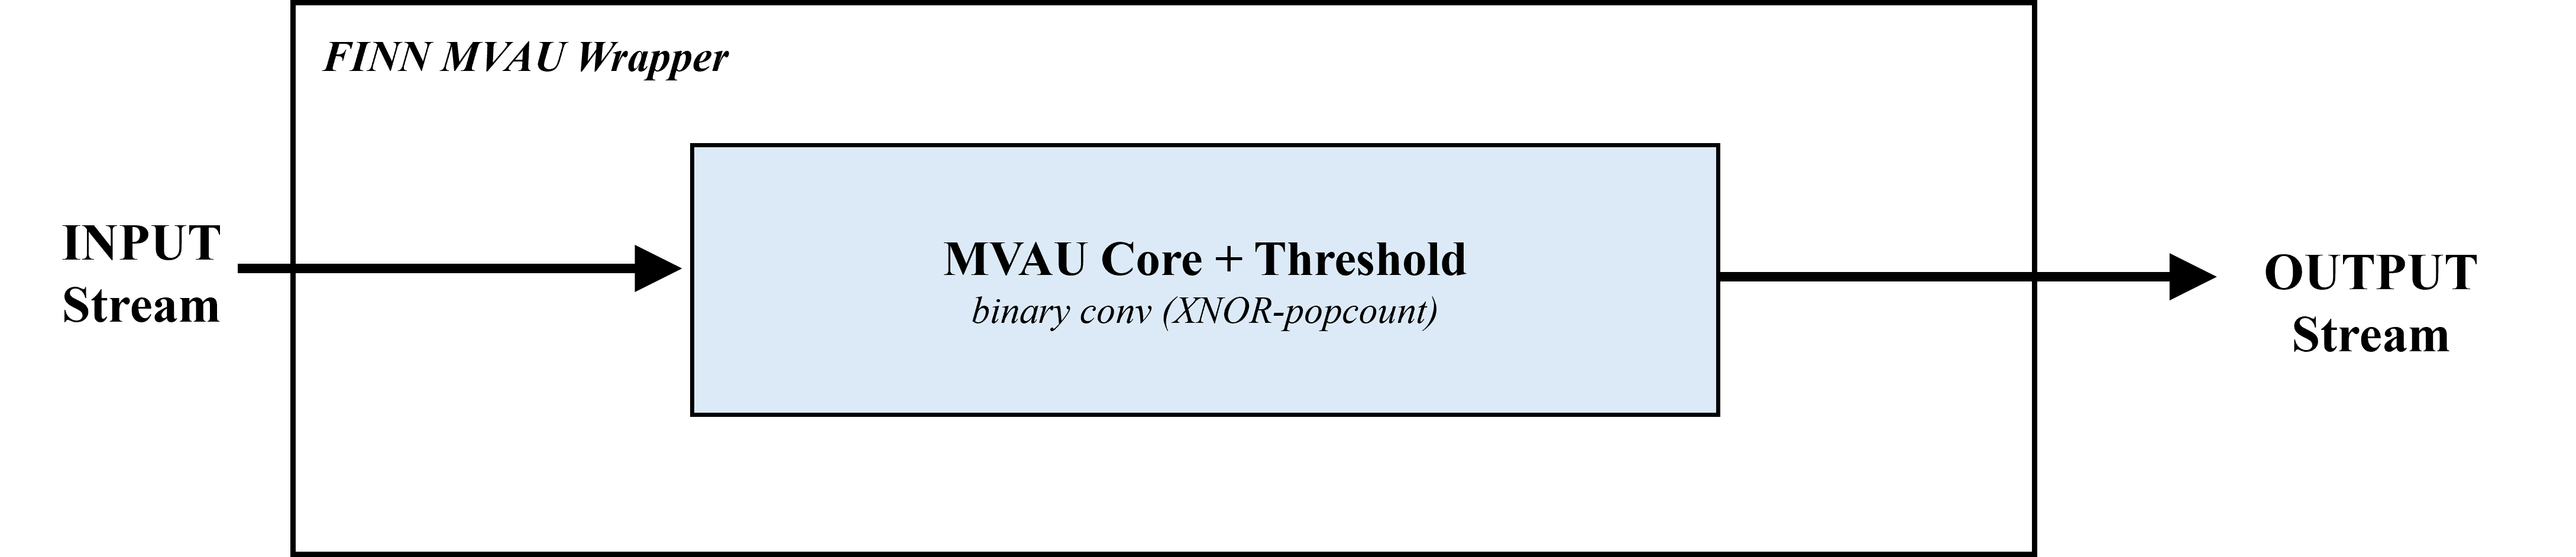
\includegraphics[width=\linewidth,keepaspectratio]{hw_finn_mvau_wrapper.png}
\caption{Internal Architecture of an Unmodified FINN MVAU.}
\label{fig:finn_mvau_orig}
\end{figure}

The Super Wrapper restructures this pipeline in two ways. First, the thresholding step is decoupled from the MVAU core: the Modified MVAU Core in Figure~\ref{fig:super_wrapper} terminates at the accumulator and exposes the raw 32-bit partial sum on its output stream. Second, an Adapter Core is added as a parallel side path with its own down/up projection RAMs; its 8-bit contribution is summed with the MVAU partial sum and only then compared against the threshold and binarised by the external Stream Adder + Threshold module. This decoupling is what makes a post-accumulator adapter possible at all on a streaming binarised pipeline.

Figure~\ref{fig:super_wrapper} shows the internal architecture of a Super Wrapper.

\begin{figure}[H]
\centering
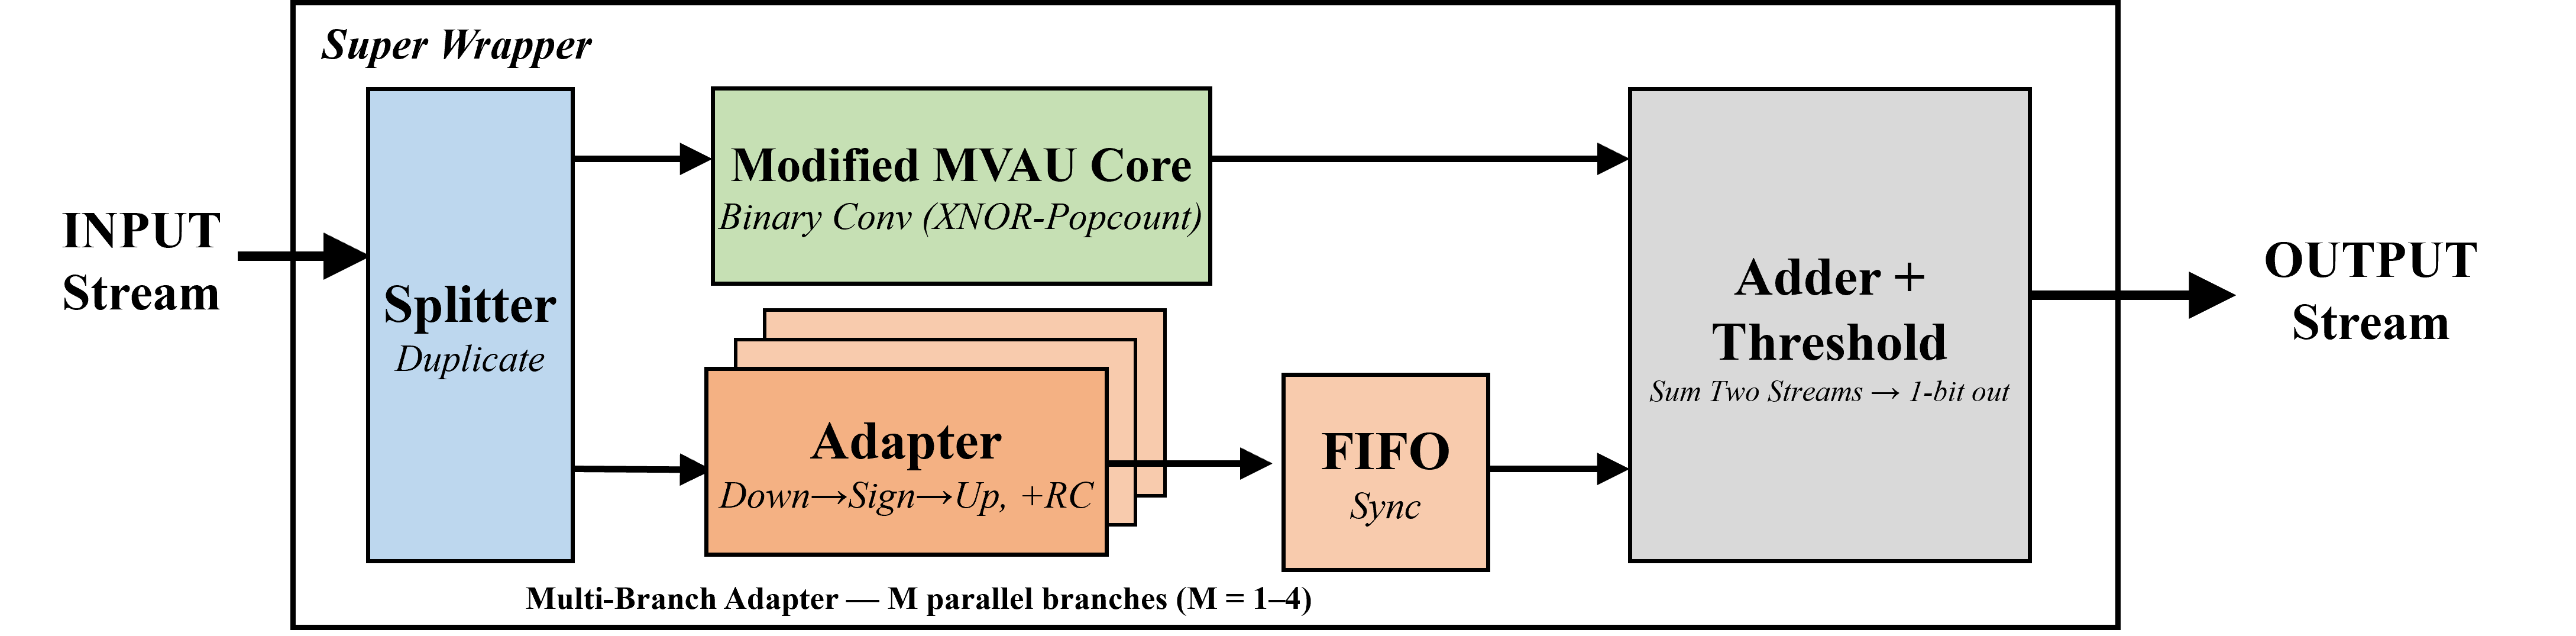
\includegraphics[width=\linewidth,keepaspectratio]{hw_super_wrapper.png}
\caption{MVAU + Adapter Super Wrapper.}
\label{fig:super_wrapper}
\end{figure}

The Super Wrapper operates as follows:

\begin{enumerate}
    \item \textbf{Stream Splitter}: Replicates the input stream to both paths using combinational logic. Both outputs must be ready before accepting input:
    \begin{equation}
    \texttt{s\_axis\_tready} = \texttt{m\_axis\_1\_tready}\ \textbf{AND}\ \texttt{m\_axis\_2\_tready}.
    \end{equation}

    \item \textbf{Path A --- MVAU Core}: The original FINN-generated MVAU core is modified to output raw partial sums (integer MAC results) \emph{before} thresholding. The internal threshold/binarization logic is decoupled from the MVAU and moved to the Stream Adder + Threshold module. This allows the adapter contribution to be fused with the MVAU result before the final binary decision.

    \item \textbf{Path B --- Adapter Core}: Executes the adapter forward computation (Algorithm~\ref{alg:adapter_forward}) using the dedicated Adapter IP (Section~\ref{sec:adapter_rtl}).

    \item \textbf{Simple FIFO}: A lightweight synchronous FIFO (depth $= 2^{6} = 64$) provides phase alignment between the MVAU and adapter paths, which have different internal pipeline depths. The FIFO absorbs the latency mismatch and ensures cycle-accurate synchronization at the fusion point.

    \item \textbf{Stream Adder + Threshold}: Fuses the MVAU partial sums with the adapter contribution and performs the final threshold comparison to produce binary output (Section~\ref{sec:adder_thresh}).
\end{enumerate}

\section{Adapter IP Internal Architecture}
\label{sec:adapter_rtl}

Figure~\ref{fig:adapter_pipeline} shows the Adapter IP: a Control Unit (FSM), the cfg-writable RAM memories (\texttt{ram\_down}, \texttt{ram\_rc}, \texttt{ram\_up}, and the contribution LUT), and the streaming datapath that performs the down-projection (XNOR-popcount), the RC-initialised accumulation, the binary sign, the up-projection (XNOR-popcount), and the $\alpha$ scaling. The down-projection path itself is pipelined over four stages (S0--S3), followed by a two-stage up-projection output path, as detailed below.

\begin{figure}[H]
\centering
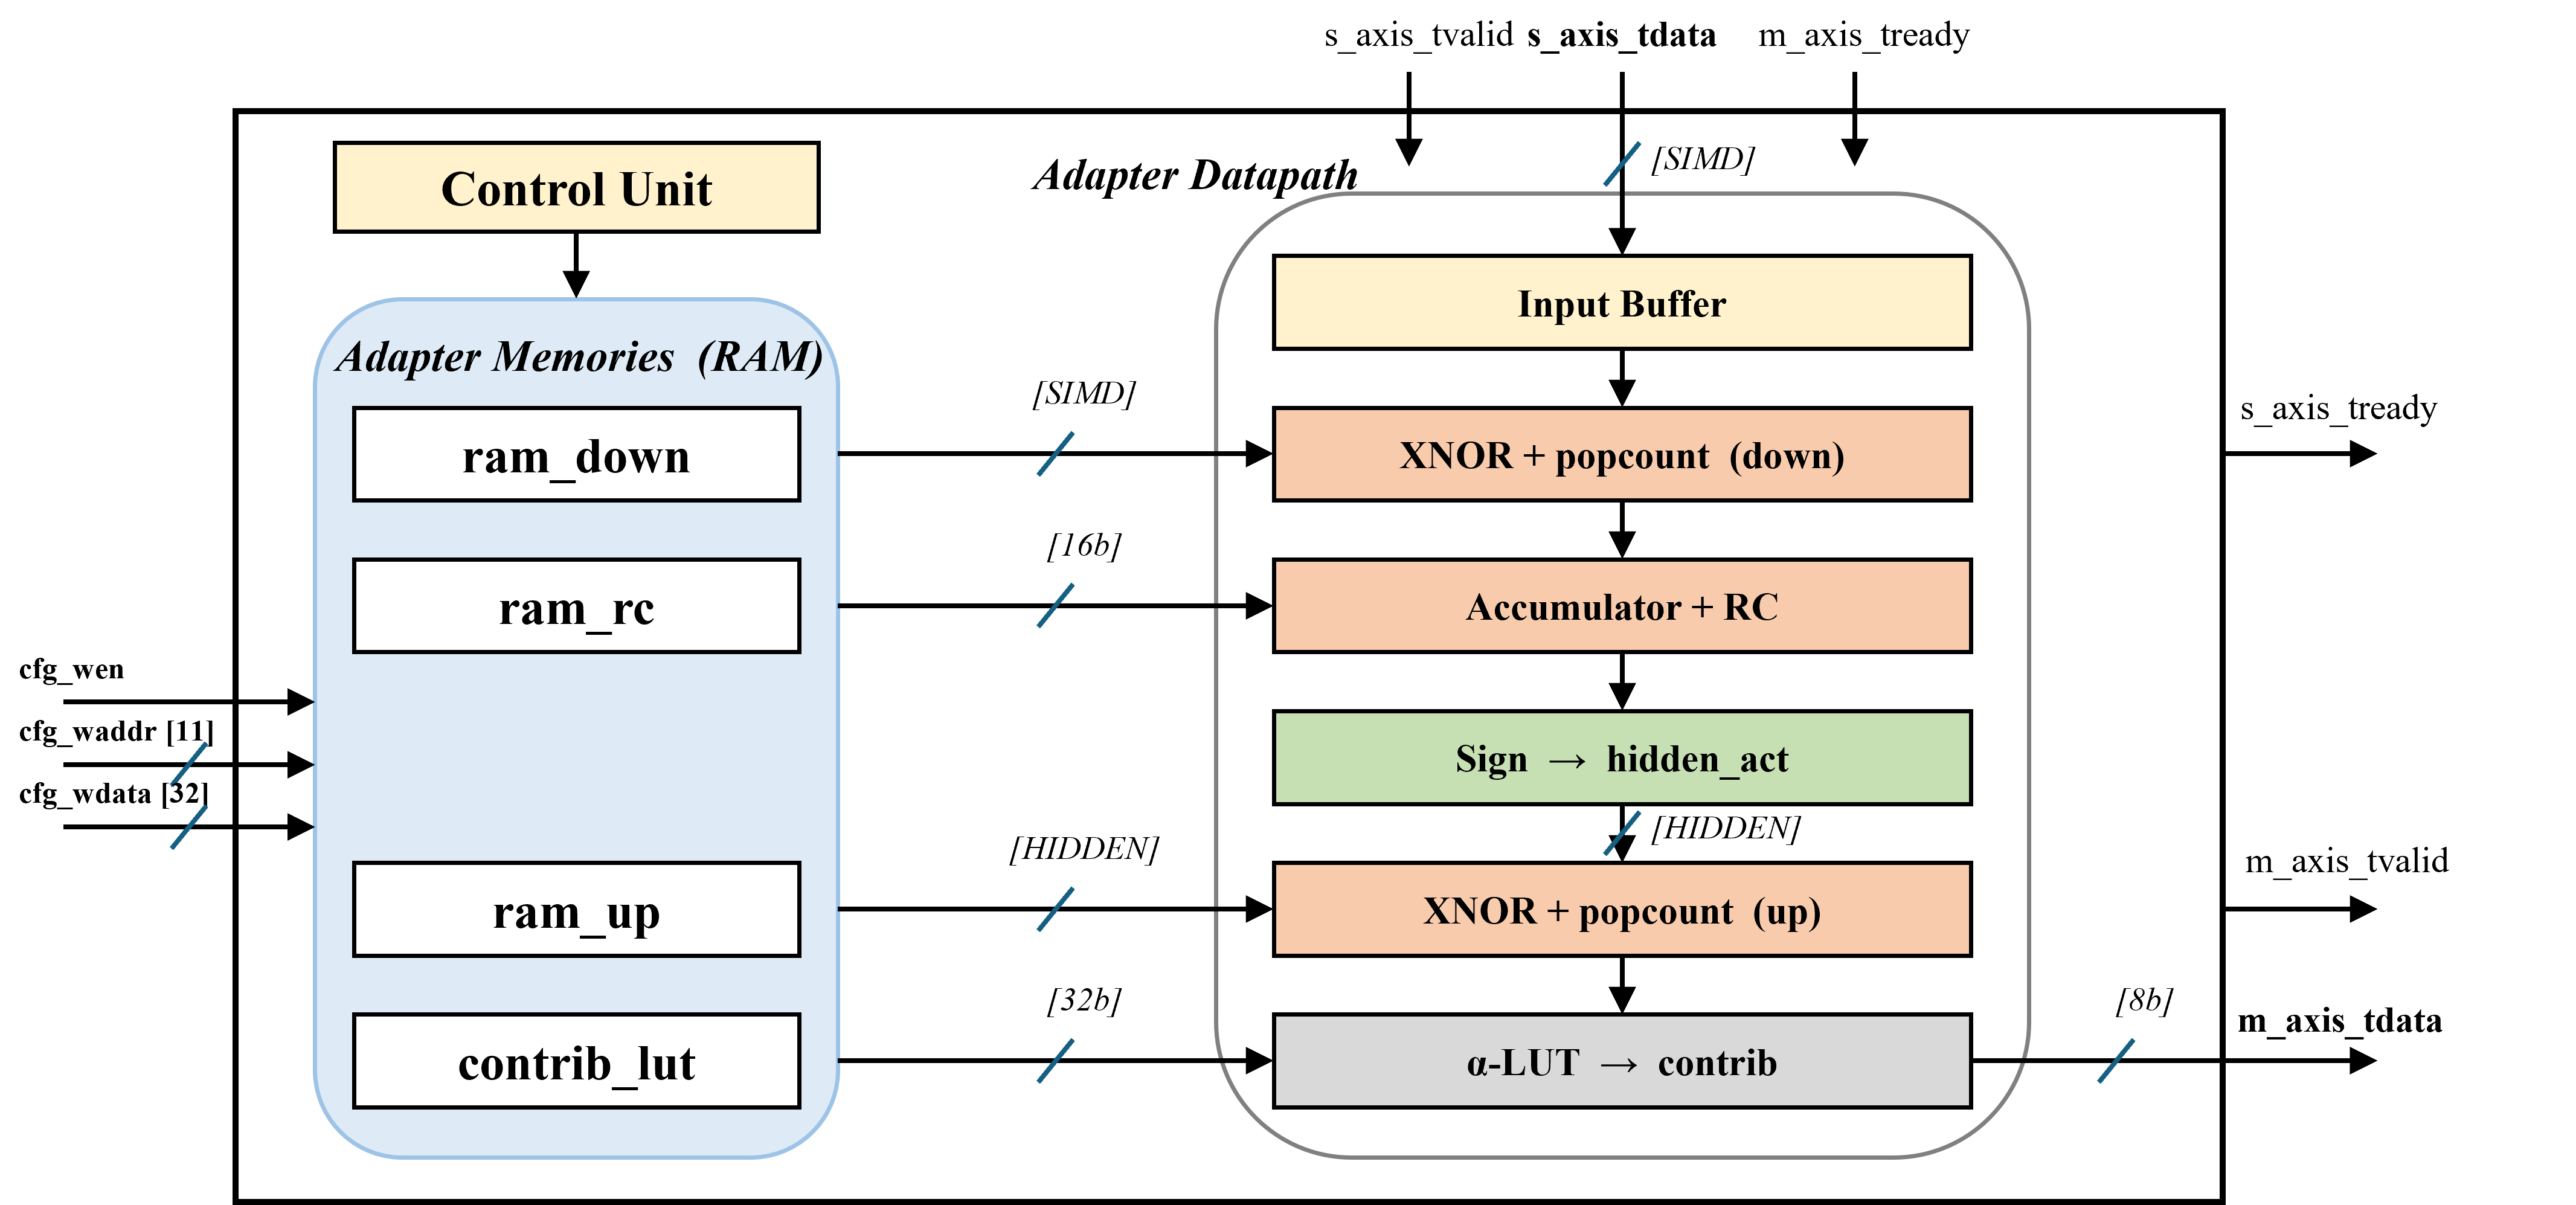
\includegraphics[width=\linewidth,keepaspectratio]{hw_adapter_internal.png}
\caption{Adapter IP Internal Architecture (One Branch Shown; Bus Labels Give Widths in Bits).}
\label{fig:adapter_pipeline}
\end{figure}

\subsection{Down-Projection Pipeline}

The down-projection path processes the center pixel of each $3 \times 3$ window through four pipeline stages:

\begin{itemize}
    \item \textbf{S0 (Input Latch + RAM Read)}: Captures the input activation and reads the corresponding down-projection weights from \texttt{ram\_down} for all $C_h$ hidden channels simultaneously.
    \item \textbf{S1 (XNOR)}: Computes $\text{XNOR}(\texttt{s1\_act}, \texttt{s1\_down[j]})$ for each hidden channel $j$.
    \item \textbf{S2 (Popcount)}: Counts the set bits of each XNOR result using a combinational adder tree inferred from the RTL popcount expression.
    \item \textbf{S3 (Accumulate)}: Adds the popcount result to the running accumulator, which was initialized with the RC bias value.
\end{itemize}

\begin{figure}[H]
\centering
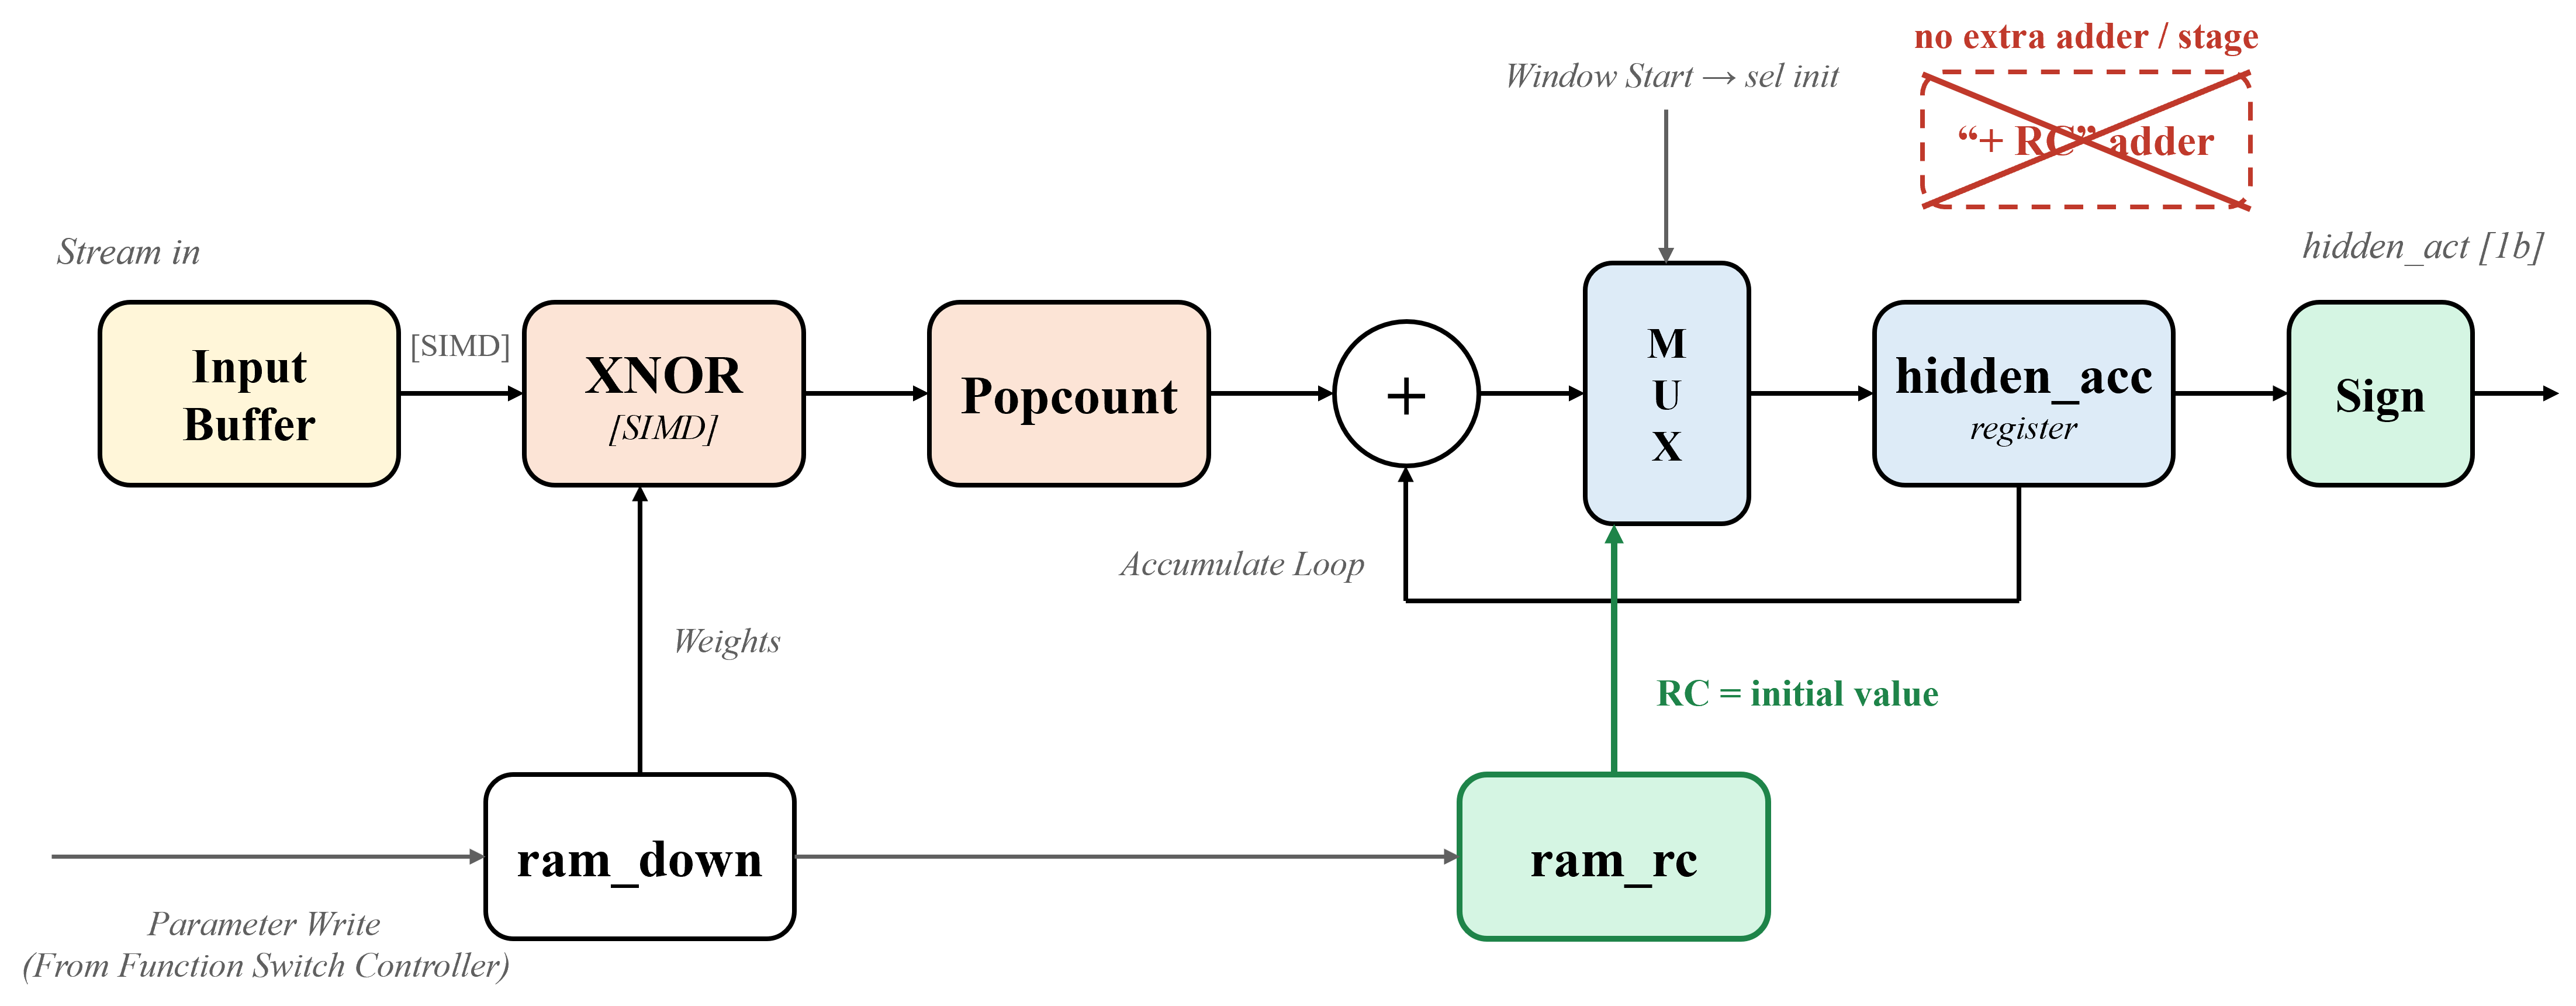
\includegraphics[width=\linewidth,keepaspectratio]{rc_in_hardware.png}
\caption[RC in Hardware: Accumulator Initialisation from \texttt{ram\_rc}]{RC in Hardware: Accumulator Initialisation from \texttt{ram\_rc} (No Extra Adder or Pipeline Stage).}
\label{fig:rc_hw}
\end{figure}

Figure~\ref{fig:rc_hw} details how RC enters this pipeline. The per-channel RC word read from \texttt{ram\_rc} drives the initialisation input of the multiplexer in front of the \texttt{hidden\_acc} register: at every window start the FSM selects this input, loading the RC bias as the accumulator's initial value in place of the constant zero; during the remaining cycles the multiplexer selects the accumulate loop, adding successive popcount results (stage S3). Because the register must load an initial value at every output window anyway, the correction introduces no additional adder, DSP slice, or pipeline stage---the crossed-out ``+RC'' stage in the figure does not exist in the RTL. The only added hardware is the \texttt{ram\_rc} storage and the initialisation-select control, both counted in the adapter overhead (Section~\ref{sec:rc}) and both runtime-writable through the Function Switch Controller (Section~\ref{sec:cfg_hub_hw}).


\subsection{Up-Projection Path}

After all input chunks are processed, the binarised hidden activation vector (\texttt{hidden\_act}) drives the up-projection:

\begin{enumerate}
    \item The up-projection weights are packed into wide RAM words. For PE $= 4$, four 32-bit weight vectors are concatenated into a single 128-bit word, enabling single-port RAM access:
    \begin{equation}
    \texttt{ram\_up[s]} = \{\mathbf{w}_{\text{up}}^{(s,3)}, \mathbf{w}_{\text{up}}^{(s,2)}, \mathbf{w}_{\text{up}}^{(s,1)}, \mathbf{w}_{\text{up}}^{(s,0)}\}.
    \end{equation}
    \item XNOR is computed between \texttt{hidden\_act} and each PE weight slice.
    \item Popcount produces the 8-bit output per PE.
\end{enumerate}

\subsection{Memory Organization}

All adapter weights use distributed RAM (LUT RAM) with the Verilog synthesis attribute \texttt{(* ram\_style = "distributed" *)}. This design choice:
\begin{itemize}
    \item Provides single-cycle read latency without BRAM pipeline overhead.
    \item Avoids consuming BRAM resources, which are reserved for the backbone MVAU weight storage.
    \item Is feasible because the projection weights are 1-bit, keeping the per-branch budget at $58{,}533$ \emph{parameters} of mixed precision (1-bit down/up projection weights plus the Int8 RC biases and the branch scale $\alpha$)---a parameter count, not a bit count.
\end{itemize}

The specific RAM configurations are summarised in Table~\ref{tab:ram_config}.

\begin{table}[H]
\centering
\caption{Adapter RAM Configurations (Example: Super4, PE$=4$)}
\label{tab:ram_config}
\resizebox{\linewidth}{!}{%
\begin{tabular}{llll}
\toprule
\textbf{RAM} & \textbf{Depth} & \textbf{Width} & \textbf{Contents} \\
\midrule
\texttt{ram\_down} & $C_h \times K = 128$ & 32 bits & Down-projection weights \\
\texttt{ram\_up}   & $C_{\text{out}}/P = 64$ & $P \times 32 = 128$ bits & Packed up-projection weights \\
\texttt{ram\_rc}   & $C_h = 32$ & 16 bits & RC bias (signed) \\
\texttt{adp\_contrib\_lut} & $2^{8} = 256$ & 32 bits (signed) & Q8-scaled adapter contribution ($\alpha$ absorbed) \\
\bottomrule
\end{tabular}%
}
\end{table}

The Int8 RC biases are sign-extended into the 16-bit \texttt{ram\_rc} words at export; the wider RAM word is layout padding for the accumulator interface, not additional numerical precision.

\section{Stream Adder + Threshold Module}
\label{sec:adder_thresh}

The Stream Adder + Threshold module fuses the MVAU partial sums with the adapter contribution and produces binary output. Its design achieves zero DSP usage through pre-computed lookup tables.

\subsection{Contribution LUT: Offline Precomputation and Runtime-Writable Storage}

The adapter output (popcount value $o_p$) must be scaled by a per-channel signed factor $\alpha$ before being added to the MVAU output. Performing this multiplication at runtime would require a DSP slice (or a costly LUT multiplier) per output channel. We avoid the multiplier entirely by representing the scaling as a lookup over the byte-wide popcount value: for each unsigned byte value $i \in [0, 255]$,
\begin{equation}
\text{LUT}[i] = \left\lfloor \frac{(i - z) \times \alpha_{Q8} + 128}{256} \right\rfloor,
\label{eq:contrib_lut}
\end{equation}
where $z$ is the zero-point (equal to $C_h/2$ for the popcount range $[0, C_h]$) and $\alpha_{Q8}$ is the Q8 quantised scale. The runtime-switching bitstream uses a \emph{dual} contribution LUT per layer---\texttt{adp\_contrib\_lut\_b0} for the lower byte of the packed adapter stream and \texttt{adp\_contrib\_lut\_b1} for the upper byte---so that two parallel sign-and-scale values can be looked up per cycle.

To support task switching without resynthesis, the LUTs are not baked in as synthesis-time constants: they are precomputed offline by the deployment-time software (which knows $\alpha$, $z$, and the per-task scaling sign) and loaded into distributed-RAM tables that remain runtime-writable through the cfg\_hub (Section~\ref{sec:cfg_hub_hw}), so switching tasks reprograms the LUT contents without rebuilding the bitstream. Both 256-deep tables live entirely in LUT-RAM---no BRAM and no DSP---and the per-channel sign selection is held in a parallel runtime-writable RAM, which also realises the inverted BatchNorm polarity of Super5 without any dedicated logic.

Conceptually, the LUT in this deployed configuration is therefore neither a strictly synthesis-time constant nor a fully runtime-derived value: it is a \emph{compile-time-defaulted, runtime-rewritable table}. The default content matches Eq.~\eqref{eq:contrib_lut} for the deployment task; per-task switching simply overwrites the 512 entries through cfg\_hub.

\subsection{Two-Stage Pipeline}

The module operates as a two-stage pipeline:

\textbf{Stage 0 (LUT Lookup + Input Capture):} When both MVAU and adapter outputs are valid:
\begin{equation}
\text{contrib}_p = \text{LUT}[\texttt{s\_axis\_2\_tdata}[(p \times 8) +: 8]], \quad p = 0, \ldots, P-1.
\end{equation}

\textbf{Stage 1 (Addition + Threshold):} The total activation is computed and compared against the per-PE threshold:
\begin{equation}
\text{total}_p = \text{mvau\_pop}_p + \text{contrib}_p,
\end{equation}
\begin{equation}
\text{out}_p = \begin{cases} 1 & \text{if } \text{total}_p \geq \text{thresh}_p[s], \\ 0 & \text{otherwise,} \end{cases}
\end{equation}
where $\text{thresh}_p[s]$ is the threshold value for PE $p$ at output step $s$, stored in per-PE threshold ROMs.

Algorithm~\ref{alg:adder_threshold} summarizes the complete fusion process.

\begin{algorithm}[htbp]
\caption{Stream Adder + Threshold Fusion}
\label{alg:adder_threshold}
\begin{algorithmic}[1]
\Require MVAU output $\mathbf{m} \in \mathbb{Z}^P$; Adapter popcount $\mathbf{o} \in [0, C_h]^P$; Threshold RAM; Contribution LUT
\Ensure Binary output $\mathbf{b} \in \{0,1\}^P$
\State \textbf{// Stage 0: LUT Lookup}
\For{$p = 0$ to $P - 1$}
    \State $\text{contrib}_p \gets \text{LUT}[o_p]$ \Comment{Pre-computed offline, runtime-rewritable}
\EndFor
\State \textbf{// Stage 1: Addition + Threshold}
\For{$p = 0$ to $P - 1$}
    \State $\text{total}_p \gets m_p + \text{contrib}_p$
    \State $b_p \gets \mathbf{1}[\text{total}_p \geq \text{thresh}_p[\text{step}]]$
\EndFor
\State \Return $\mathbf{b}$
\end{algorithmic}
\end{algorithm}

\section{Runtime Configuration Hub (\texorpdfstring{cfg\_hub}{cfg\_hub})}
\label{sec:cfg_hub_hw}

To enable a single compiled bitstream to serve multiple downstream tasks at runtime, MARS inserts a lightweight configuration hub into the streaming dataflow partition. The feasibility rests on a simple observation: when downstream tasks share the same 1W1A VGG-like backbone, the binary convolution and FC weights are identical; only the BatchNorm-fused thresholds, the classifier output-projection weights, and the five adapter blobs (enable, down/up projection RAM, RC bias, threshold, sign, contribution LUT) differ. Per downstream task, this reduces the task-dependent state to a host-side blob of 25{,}088 bytes ($\approx$25~KB), transferred as 6{,}757 32-bit cfg-hub word-writes ($27{,}028$ bytes of bus payload; fields narrower than 32 bits, such as the byte-packed classifier weights, are widened to full words on the bus). The hub (\texttt{adapter\_cfg\_hub.v}) occupies a 64~KB \emph{address} aperture at base address \texttt{0x40010000}---this is the size of the addressable window in the system memory map, not the amount of data transferred; only the $\approx$25~KB blob above is actually written per task, sparsely across the aperture. The 64~KB is decoded from the 16-bit byte address as a 3-bit unit select (\texttt{byte\_addr[15:13]}) and an 11-bit word address (\texttt{byte\_addr[12:2]}). Figure~\ref{fig:cfghub_sys} shows the system-level integration: the micro-processor writes to the control interface of the hub, which combinationally demultiplexes---through a 3-bit unit select whose unit 0 is further split into a low and a high half---to nine physical destinations distributed across the pipeline (eight address units, nine destinations). No data path is perturbed; the entire switching infrastructure is orthogonal to the streaming dataflow.

\begin{figure}[H]
\centering
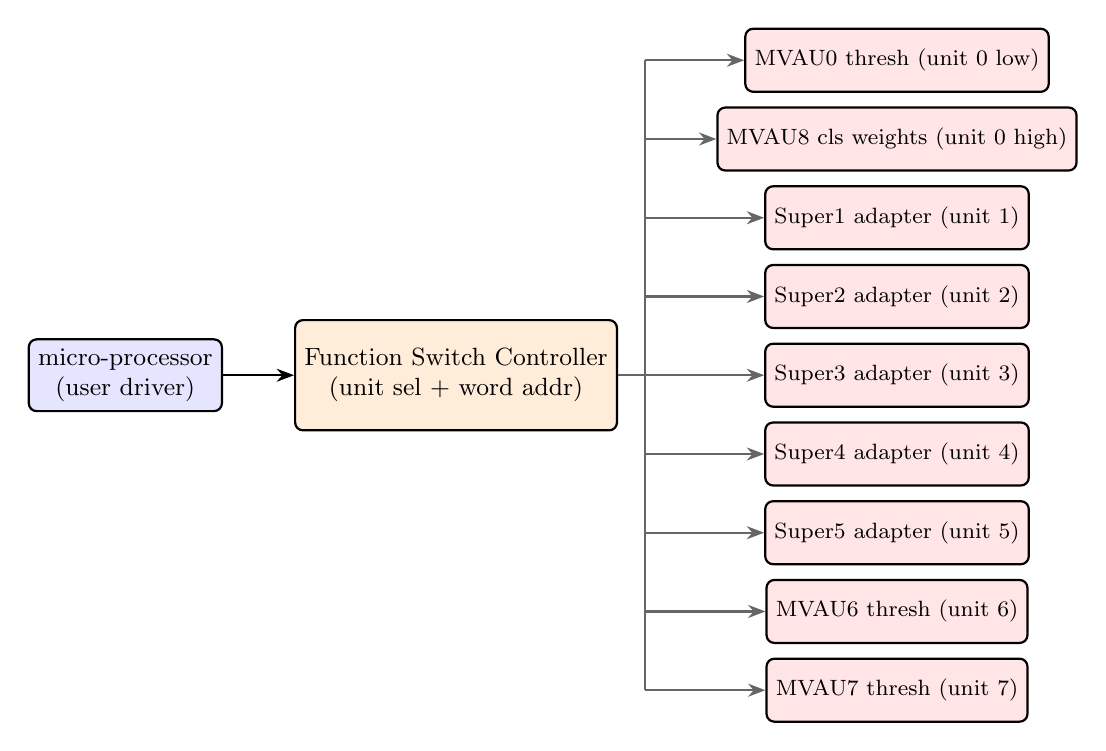
\begin{tikzpicture}[
    font=\small,
    ps/.style={rectangle, draw, thick, rounded corners=1mm, fill=blue!10, minimum width=2.2cm, minimum height=0.9cm, align=center},
    hub/.style={rectangle, draw, thick, rounded corners=1mm, fill=orange!15, minimum width=3.4cm, minimum height=1.4cm, align=center},
    mod/.style={rectangle, draw, thick, rounded corners=1mm, fill=red!10, minimum width=2.0cm, minimum height=0.8cm, align=center, font=\footnotesize},
    arr/.style={-{Stealth[length=2.2mm]}, thick}
]
\node[ps] (ps) at (0,0) {micro-processor\\(user driver)};
\node[hub] (hub) at (4.2,0) {Function Switch Controller\\(unit sel + word addr)};
\draw[arr] (ps.east) -- (hub.west);

\node[mod] (u0l) at (9.8, 4.0) {MVAU0 thresh (unit 0 low)};
\node[mod] (u0h) at (9.8, 3.0) {MVAU8 cls weights (unit 0 high)};
\node[mod] (s1)  at (9.8, 2.0) {Super1 adapter (unit 1)};
\node[mod] (s2)  at (9.8, 1.0) {Super2 adapter (unit 2)};
\node[mod] (s3)  at (9.8, 0)   {Super3 adapter (unit 3)};
\node[mod] (s4)  at (9.8,-1.0) {Super4 adapter (unit 4)};
\node[mod] (s5)  at (9.8,-2.0) {Super5 adapter (unit 5)};
\node[mod] (u6)  at (9.8,-3.0) {MVAU6 thresh (unit 6)};
\node[mod] (u7)  at (9.8,-4.0) {MVAU7 thresh (unit 7)};

\draw[black!60, thick] (hub.east) -- (6.6,0);
\draw[black!60, thick] (6.6,4.0) -- (6.6,-4.0);
\foreach \t in {u0l, u0h, s1, s2, s3, s4, s5, u6, u7} {
    \draw[arr, black!60] (6.6,0 |- \t.west) -- (\t.west);
}
\end{tikzpicture}
\caption{System-Level Integration of the Function Switch Controller.}
\label{fig:cfghub_sys}
\end{figure}

Figure~\ref{fig:fsc_circuit} details the internal circuit of the Function Switch Controller. An AW latch captures the 16-bit AXI-Lite write address while the write FSM tracks the AWVALID/WVALID handshakes, dispatching the write and returning BRESP once both address and data have arrived. The latched address is decomposed combinationally into the unit decode (\texttt{a[15:13]}), the unit-0 split (\texttt{a[12]}), and the word slice (\texttt{a[12:2]}); a 1-of-9 write-enable demultiplexer turns the decoded unit into a single-cycle WEN pulse, while the shared configuration bus (\texttt{waddr}\,$\cdot$\,\texttt{wdata}) is broadcast to all nine destinations (MVAU0 thresholds, MVAU8 classifier weights, the Super1--5 adapters, and the MVAU6/MVAU7 thresholds)---only the unit whose WEN is asserted commits the write.

\begin{figure}[H]
\centering
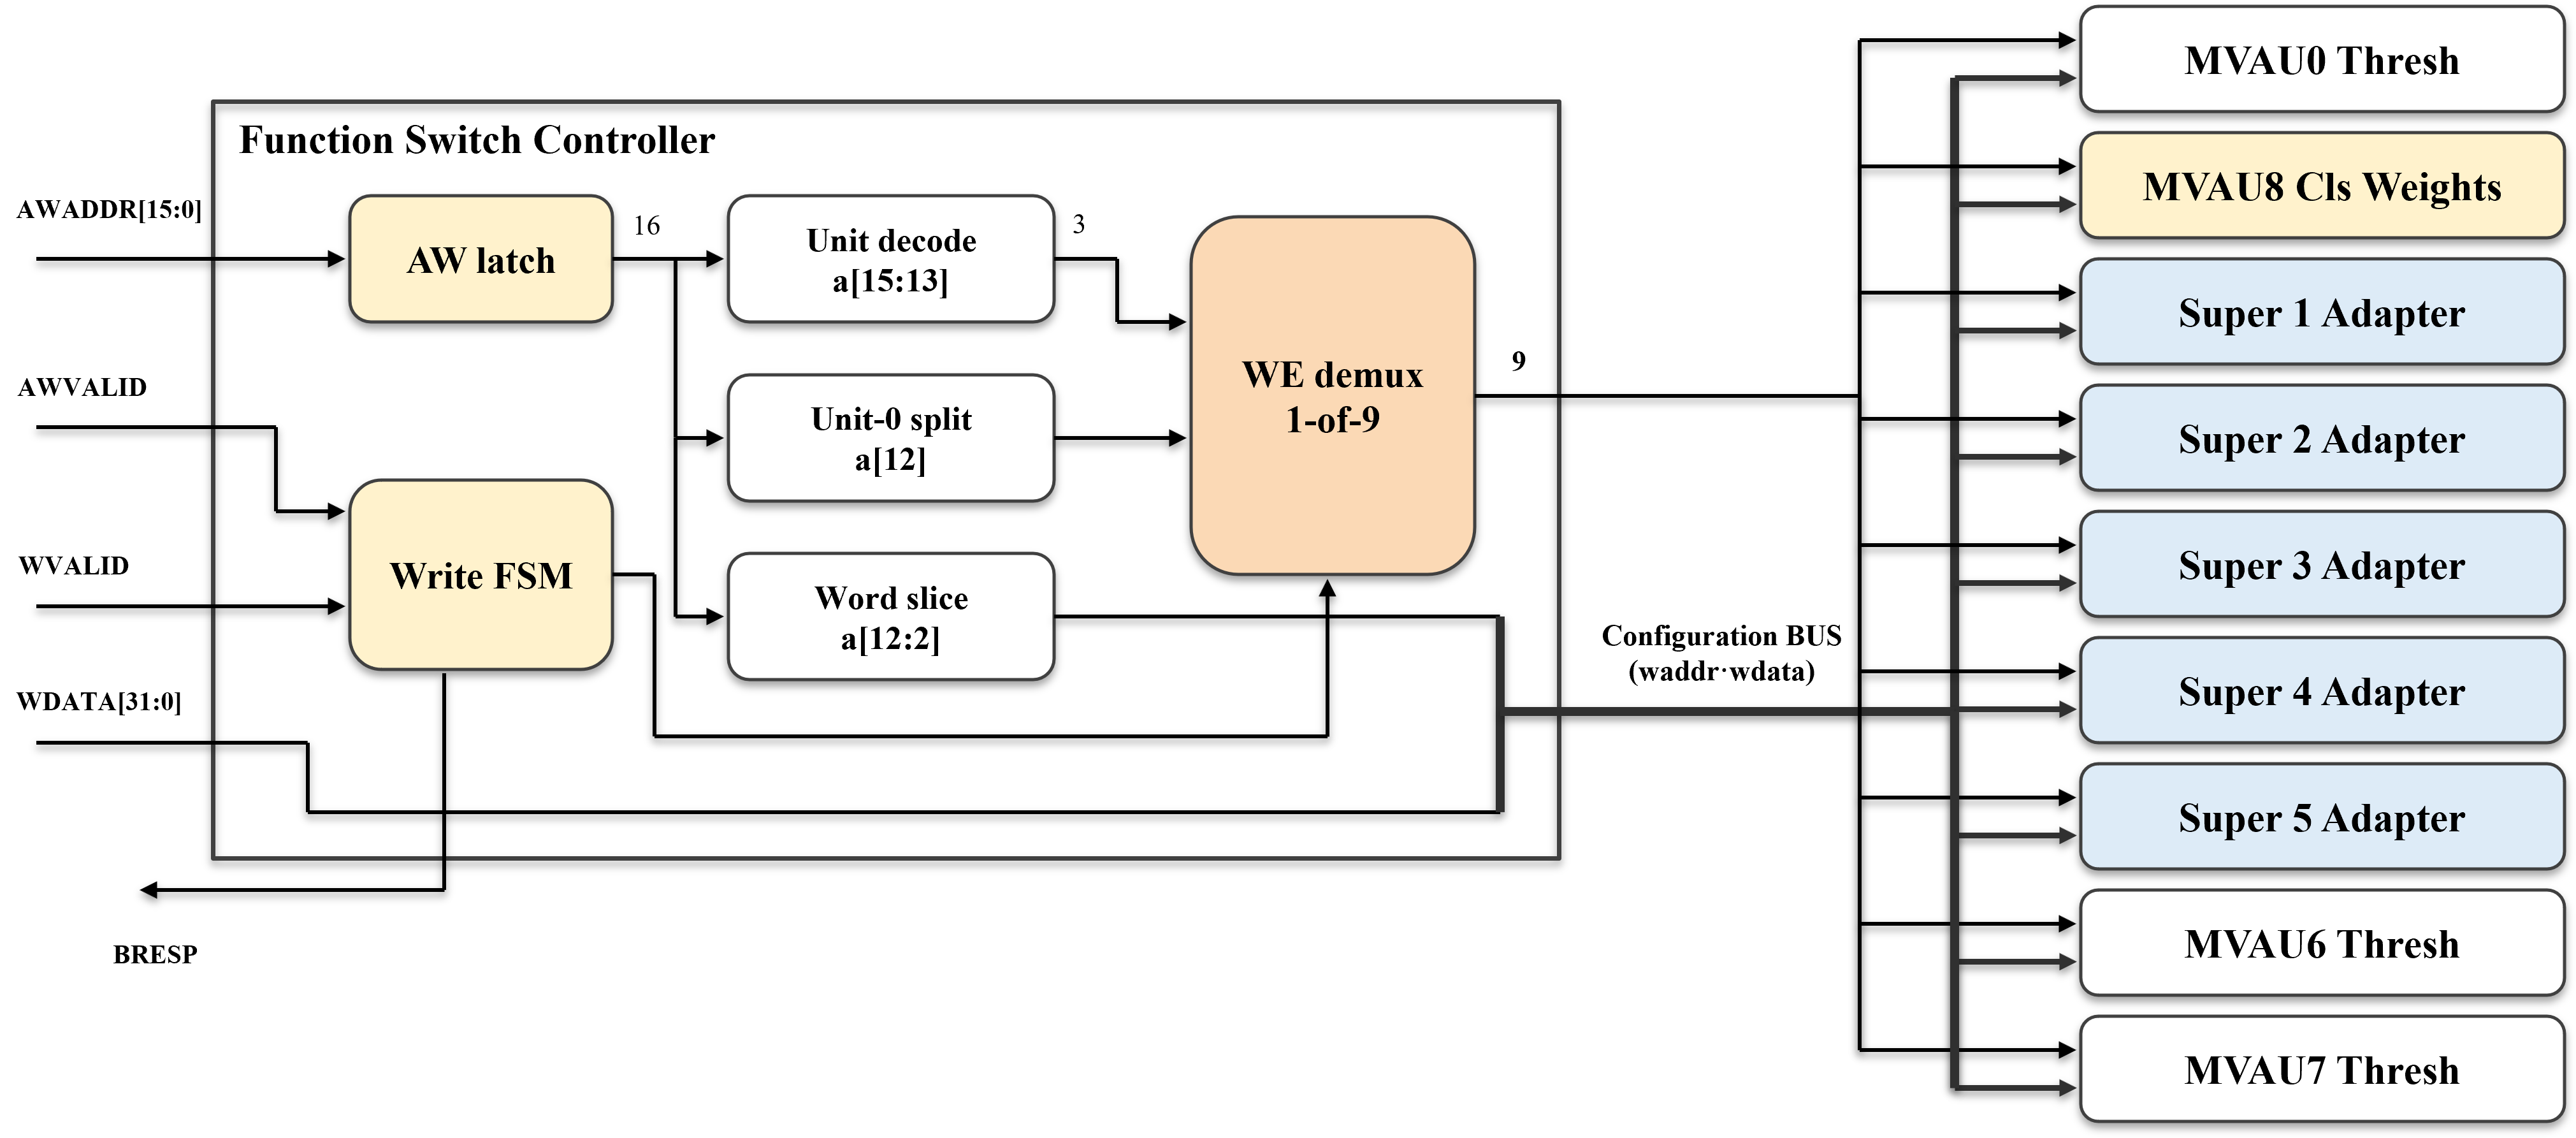
\includegraphics[width=\linewidth,keepaspectratio]{fsc_circuit.png}
\caption{Internal Circuit of the Function Switch Controller.}
\label{fig:fsc_circuit}
\end{figure}

\subsection{Address Map}

Figure~\ref{fig:cfghub_map} visualises the 64~KB aperture. Each 8~KB slot covers either one MVAU's threshold block or a module's adapter registers (enable at word~0, Q8 thresholds at word~1152, sign bits at word~1408), or a block of per-task parameters (MVAU0 thresholds, MVAU8 classifier weights, MVAU6/MVAU7 thresholds).

\begin{figure}[H]
\centering
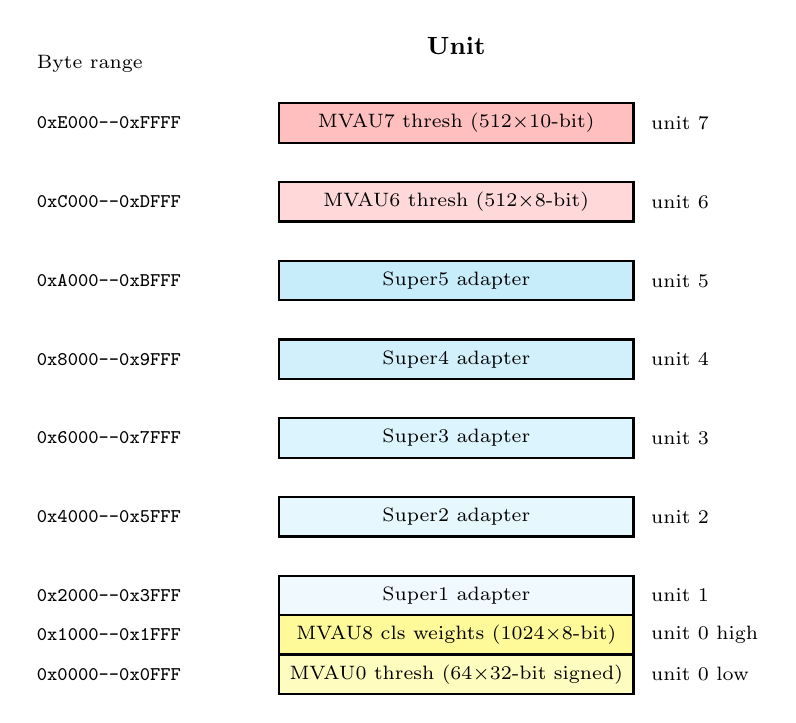
\begin{tikzpicture}[font=\footnotesize]
\foreach \y/\range/\label/\col in {%
    7/0xE000--0xFFFF/MVAU7 thresh (512$\times$10-bit)/red!25,
    6/0xC000--0xDFFF/MVAU6 thresh (512$\times$8-bit)/red!15,
    5/0xA000--0xBFFF/Super5 adapter/cyan!22,
    4/0x8000--0x9FFF/Super4 adapter/cyan!18,
    3/0x6000--0x7FFF/Super3 adapter/cyan!14,
    2/0x4000--0x5FFF/Super2 adapter/cyan!10,
    1/0x2000--0x3FFF/Super1 adapter/cyan!6,
    0.5/0x1000--0x1FFF/MVAU8 cls weights (1024$\times$8-bit)/yellow!40,
    0/0x0000--0x0FFF/MVAU0 thresh (64$\times$32-bit signed)/yellow!25
} {
    \draw[fill=\col, thick] (0,\y) rectangle (4.5,\y+0.5);
    \node[anchor=west, font=\scriptsize\ttfamily] at (-3.2,\y+0.25) {\range};
    \node[font=\scriptsize] at (2.25,\y+0.25) {\label};
}
\node[font=\small\bfseries, anchor=south] at (2.25, 8) {Unit};
\node[anchor=west, font=\scriptsize] at (-3.2, 8) {Byte range};
\foreach \y/\u in {0/0 low, 0.5/0 high, 1/1, 2/2, 3/3, 4/4, 5/5, 6/6, 7/7} {
    \node[anchor=west, font=\scriptsize] at (4.6,\y+0.25) {unit \u};
}
\end{tikzpicture}
\caption{\texttt{cfg\_hub} 64\,KB Address Map.}
\label{fig:cfghub_map}
\end{figure}

\subsection{Runtime Switching Sequence}

Figure~\ref{fig:runtime_seq} summarises the end-to-end switching flow. The pre-condition for a switch is that the Output DMA \texttt{done} bit is asserted, guaranteeing the previous inference batch has been drained from the streaming pipeline (empirical validation in Section~\ref{sec:runtime_switch}). The user driver then performs a bulk MMIO write of the task-specific parameter blob ($\approx$6{,}757 words, $1.86$~ms rewrite; post-switch correctness verified separately), after which the next batch may be launched immediately; no explicit pipeline flush is required. The user-space driver maps the cfg\_hub aperture once at start-up and issues the 6{,}757 word-writes as a few contiguous bulk MMIO transfers rather than word-by-word calls; minimising this per-write software overhead is what makes the $1.86$~ms configuration-rewrite latency reported in Section~\ref{sec:runtime_switch} achievable.

\begin{figure}[H]
\centering
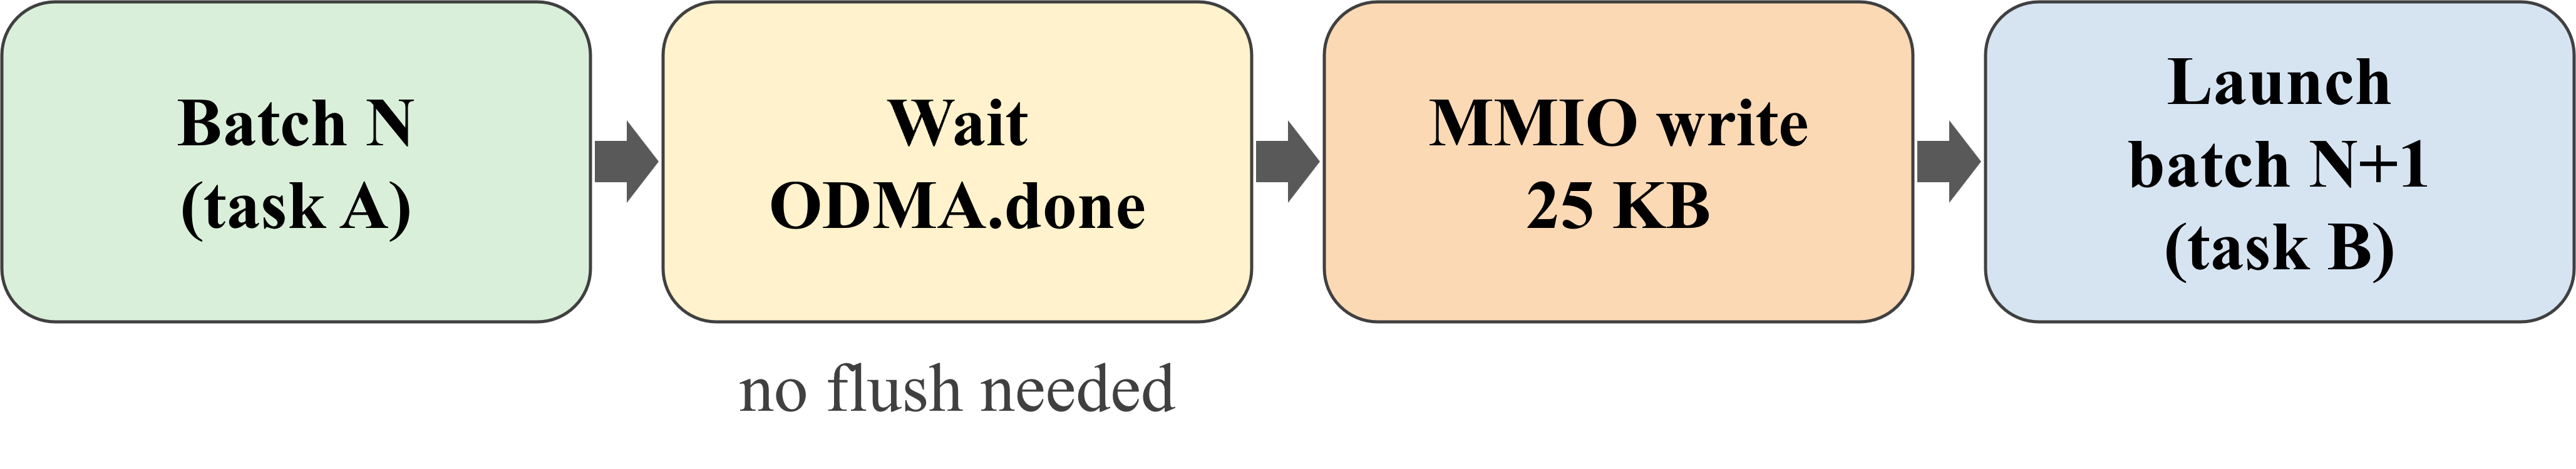
\includegraphics[width=\linewidth,keepaspectratio]{task_switch.png}
\caption{End-to-End Runtime Task-Switching Sequence.}
\label{fig:runtime_seq}
\end{figure}

\subsection{RTL Modifications}

Three RTL modifications enable the above flow without disturbing the streaming dataflow:
\begin{itemize}
    \item \textbf{MVAU0}: the 16 hard-coded threshold multiplexers are replaced with 16 distributed-RAM banks, each exposing a write port to \texttt{cfg\_hub}.
    \item \textbf{Super1--5 Stream Adder + Threshold}: the Q8 threshold RAM and sign-polarity bits become cfg-writable distributed RAM, and an \texttt{adapter\_enable} register at word 0 gates the adapter contribution so that Super1--5 can revert to pure backbone behaviour (used for the CIFAR-10 mode).
    \item \textbf{Classifier memstream} (MVAU8): a cfg$\to$memstream state machine inside the \texttt{\_imp} wrapper drives the on-chip memstream, enabling runtime reload of the output projection weights that differ between CIFAR-10 and SVHN.
\end{itemize}

Because the shared backbone is frozen once and the persistent per-task blobs are stored off-chip and copied into the cfg-writable on-chip memories at switch time, MARS's deployed fabric cost is independent of the number of deployed tasks---a single bitstream serves them all ($O(1)$), with no change to the fabric floorplan. Prior task-switching approaches instead pay a per-task or per-variant deployment cost, although it manifests differently per family: partial-reconfiguration designs require one additional partial bitstream (\texttt{.bit}) per task and a more complex fabric floorplan (reconfigurable regions), while on-chip model-selection designs keep a fixed synthesis-time variant set resident on-chip and multiplex the selected variant's parameters into a shared array. Figure~\ref{fig:scaling_cost} illustrates this contrast schematically.

\begin{figure}[H]
\centering
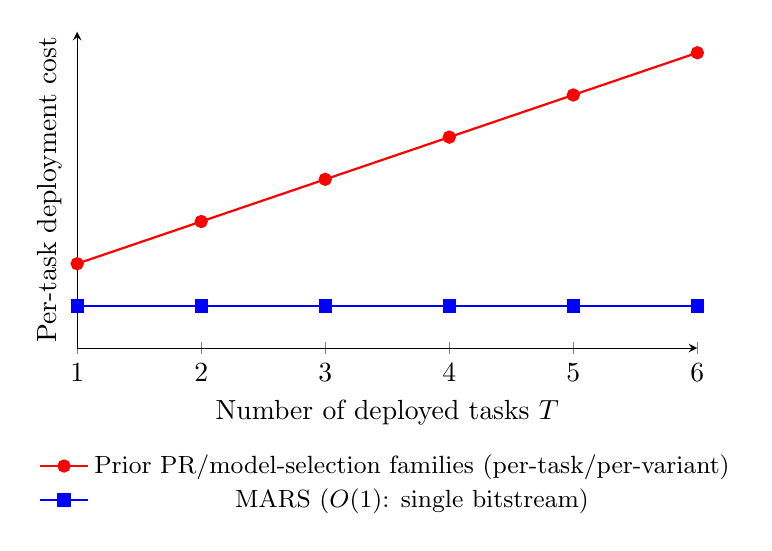
\begin{tikzpicture}
\begin{axis}[
    width=0.78\textwidth, height=5.6cm,
    xlabel={Number of deployed tasks $T$}, ylabel={Per-task deployment cost},
    xmin=1, xmax=6, ymin=0, ymax=7.5,
    xtick={1,2,3,4,5,6}, ytick=\empty,
    axis lines=left,
    legend style={font=\small, at={(0.5,-0.30)}, anchor=north, draw=none},
    domain=1:6, samples=6,
]
\addplot[thick, red, mark=*] {1+x};
\addlegendentry{Prior PR/model-selection families (per-task/per-variant)}
\addplot[thick, blue, mark=square*] {1};
\addlegendentry{MARS ($O(1)$: single bitstream)}
\end{axis}
\end{tikzpicture}
\caption[Conceptual Deployment Cost vs.\ Task/Variant Count]{Conceptual Deployment Cost vs.\ Task/Variant Count: MARS $O(1)$ On-Chip vs.\ Prior Per-Task/Per-Variant Cost (Qualitative; Quantitative Axes Tabulated in Tables~\ref{tab:prior_multitask}--\ref{tab:reconfig_ctrl}).}
\label{fig:scaling_cost}
\end{figure}

\section{Pipelining of the MVAU + Adapter Integrated System}
\label{sec:simd_pipeline}

The backbone MVAU pipelining and the per-layer PE/SIMD folding follow the standard FINN streaming-dataflow scheme~\cite{Umuroglu2017FINN, Blott2018FINNR}; neither is claimed as a contribution of this thesis. What is specific to MARS is integrating the adapter side-stream into this folded datapath without breaking it: the Adapter IP and the Stream Adder + Threshold module are pipeline-staged (Sections~\ref{sec:adapter_rtl}--\ref{sec:adder_thresh}) and synchronised with the exposed MVAU partial-sum stream through per-layer FIFOs, so that the integrated system still closes timing at 100~MHz under the FINN-selected folding and the adapter-enabled throughput stays within $\approx$0.5\% of the bare backbone (Section~\ref{sec:cross_platform}). The per-layer folding factors of the throughput and compactness builds are reported as measured data in Section~\ref{sec:pe_simd_breakdown} (Table~\ref{tab:pe_simd_config}).

\section{Verification Methodology}

The verification strategy employs a three-level hierarchical approach covering per-module RTL simulation, top-level streaming dataflow simulation, and end-to-end on-board validation:

\begin{enumerate}
    \item \textbf{Module-level RTL simulation}: Each Super Wrapper (Super1--Super5) is tested independently against golden vectors produced by a bit-exact software model of the hardware computation (XNOR-popcount, accumulation, Q8 threshold comparison, sign/polarity handling). The golden model reads the same hardware-layout weight images that initialise the FPGA RAMs, rather than recomputing from the pre-export software tensors---this eliminates representation-mismatch false failures at the bit level. The backbone weights themselves are identical across tasks; adapter training never updates them. Across the five modules the simulations cover 43{,}520 test vectors in total (the per-channel outputs over each layer's output footprint, folded by the PE factors of Table~\ref{tab:pe_simd_config}), with 100\% pass on every module.

    \item \textbf{Top-level dataflow simulation}: The complete streaming pipeline---Input DMA, MVAU0, the five adapter-enhanced Super Wrappers (Super1--5), MaxPool, MVAU6--MVAU8, LabelSelect, Output DMA---is simulated as a single block design driving a batch of SVHN test images through the full dataflow. Classification decisions match the PyTorch golden reference, confirming software-consistent behaviour of the adapter integration, FIFO synchronisation, and Stream Adder + Threshold fusion at the system level.

    \item \textbf{End-to-end on-board verification}: The generated bitstream is loaded onto the target FPGA, and 10{,}000 SVHN test images are processed at batch size 1000 using the Python validation driver (mean of 10 runs). This throughput build is the throughput/energy measurement configuration: 1{,}866~img/s end-to-end (1{,}933~img/s driver + FPGA only), amortised per-image time averaging 0.54~ms at batch size 1000. \emph{On-board accuracy correctness} is established by the N-task compactness build on the canonical \texttt{cifar10\_1w1a} backbone in Section~\ref{sec:pe1_3ds} (within $0.69$~pp of software across five datasets, Table~\ref{tab:pe1_3ds_acc}); the same cfg\_hub reconfiguration mechanism is exercised there in adapter-disabled mode, confirming that runtime threshold reload introduces no additional numerical error.
\end{enumerate}

% ==========================================================
% Chapter 5: Experiments and Evaluation
% ==========================================================
\chapter{Experiments and Evaluation}
\label{ch:experiments}

This chapter presents the experimental evaluation of the MARS accelerator across five dimensions: software-side transfer learning accuracy (Section~\ref{sec:sw_results}), FPGA resource utilisation and power (Section~\ref{sec:hw_results}), cross-platform performance comparison (Section~\ref{sec:cross_platform}), runtime task switching and N-task deployment (Section~\ref{sec:runtime_switch}), and task-switching scaling analysis (Section~\ref{sec:scaling}).

\section{End-to-End Design Flow}
\label{sec:design_flow}

Figure~\ref{fig:design_flow} shows the end-to-end software-to-hardware flow of MARS. On the software side, a shared 1W1A VGG-like backbone is frozen while a Multi-Branch Adapter (with RC) is trained per task ($\#1\,\ldots\,\#N$); the model is built, trained, and evaluated on the target datasets. The FINN compiler then generates the Backbone IP, which is deployed to hardware, where the custom Adapter IP is fused into the backbone and a Runtime Function Switch Controller provides single-bitstream task switching. The procedure decomposes into six stages:

\begin{enumerate}
    \item \textbf{Stage 1 --- Backbone Pre-training}: The VGG-like backbone (6 conv + 3 FC layers) is trained on CIFAR-10 using PyTorch with 1W1A quantisation-aware training. Weights are quantised to $\{-1, +1\}$ (1-bit signed), activations to $\{-1, +1\}$ (1-bit signed), and input to 8-bit (Q1.7 format) \cite{Umuroglu2017FINN, Jacob2018Quantization}.

    \item \textbf{Stage 2 --- Adapter Fine-tuning}: The backbone weights are frozen. Only the adapter parameters (down/up projection weights, RC biases, and scaling factors $\alpha$) are trained on the target dataset (SVHN or FashionMNIST). Checkpoint selection follows the original BNN-PYNQ trainer flow: the model is evaluated after every epoch and the highest-scoring epoch is retained (\texttt{best.tar}); this per-epoch evaluation uses the \emph{test} split, so all reported accuracies are best-epoch operating points selected on the test set. Because every configuration ($M{=}1$--$4$, with/without RC, all backbones and targets) uses the identical rule, the comparisons are procedurally consistent, although best-epoch selection on the test split may bias both absolute accuracies and relative differences; absolute accuracies should be read as operating-point upper bounds rather than held-out estimates.

    \item \textbf{Stage 3 --- Weight Export}: Backbone weights are exported in the FINN interleaved format. Adapter weights are converted to hexadecimal \texttt{.dat} files for RAM initialization, with PE-aligned packing for the up-projection weights.

    \item \textbf{Stage 4 --- FINN Backbone Generation}: The FINN framework converts the quantised backbone into a streaming dataflow accelerator, generating HLS-based MVAU IP cores with streaming interfaces.

    \item \textbf{Stage 5 --- RTL Integration}: The FINN-generated MVAU modules are replaced with Super Wrappers at the RTL block-design level. The original MVAU internal threshold logic is decoupled, and the custom Adapter IP, Stream Splitter, FIFO, and Stream Adder + Threshold modules are connected.

    \item \textbf{Stage 6 --- FPGA Verification}: The integrated design is synthesized, placed, and routed. A golden model is established in Python, and the FPGA output is compared bit-by-bit against the golden reference. The per-module datapath is verified bit-exact (43{,}520 vectors, 100\% pass); at the full 10{,}000-image end-to-end level the on-board result reproduces the software reference to within $0.69$~pp (Table~\ref{tab:pe1_3ds_acc}), the small residual being consistent with Q8 threshold-rounding accumulation rather than a bit-level error.
\end{enumerate}

\begin{figure}[H]
\centering
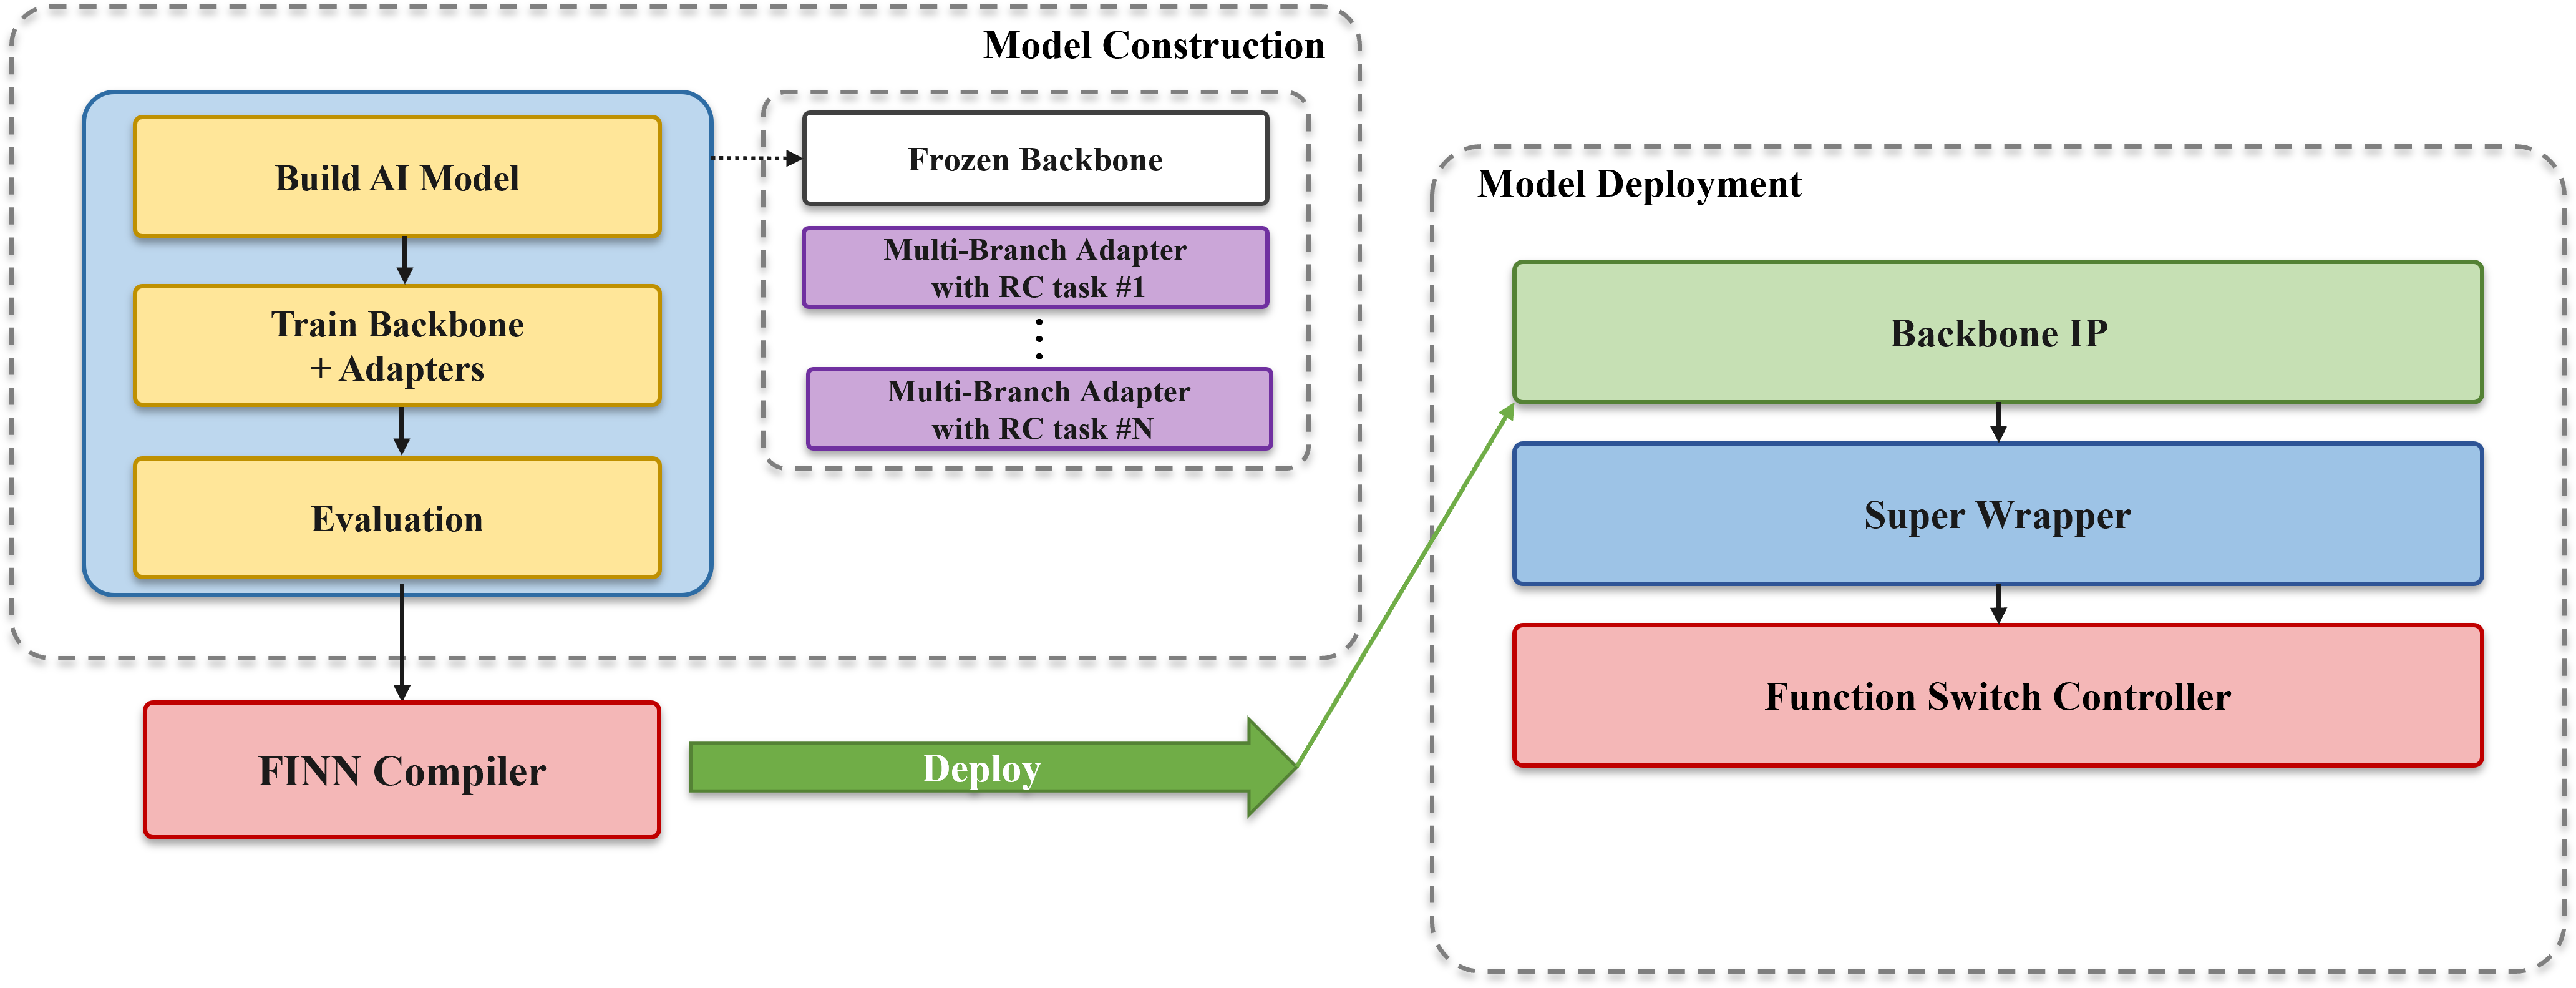
\includegraphics[width=\linewidth,keepaspectratio]{hw_end2end.png}
\caption{End-to-End Software-to-Hardware Flow of MARS.}
\label{fig:design_flow}
\end{figure}

\section{Experimental Setup}

\subsection{Datasets and Tasks}

This thesis uses five $32\times32$-class image-classification datasets, summarised in Table~\ref{tab:datasets}. Each can serve either as the frozen \emph{backbone} (source)---pre-trained once and then held fixed---or as a downstream \emph{target} that is adapted to. They span deliberately different visual domains: general natural objects (CIFAR-10, STL10, CINIC10), street-view digits (SVHN), and grayscale clothing (FashionMNIST), so that transfer is exercised both within and across domains.

\begin{table}[H]
\centering
\caption{Datasets Used in This Thesis (All Adapted to a $32\times32\times3$ Input).}
\label{tab:datasets}
\resizebox{\linewidth}{!}{%
\begin{tabular}{lccccl}
\toprule
\textbf{Dataset} & \textbf{Classes} & \textbf{Train / Test} & \textbf{Native Res.} & \textbf{Modality} & \textbf{Domain / Notes} \\
\midrule
CIFAR-10     & 10 & 50{,}000 / 10{,}000 & $32\times32$ & RGB & general natural objects (default backbone) \\
SVHN         & 10 & 73{,}257 / 26{,}032 & $32\times32$ & RGB & street-view house-number digits \\
STL10        & 10 & 5{,}000 / 8{,}000 & $96\times96$ & RGB & ImageNet-derived objects (downscaled) \\
FashionMNIST & 10 & 60{,}000 / 10{,}000 & $28\times28$ & grayscale & clothing (resized, channel-replicated) \\
CINIC10      & 10 & 90{,}000 / 90{,}000 & $32\times32$ & RGB & CIFAR-10 + downsampled ImageNet; 270k total (90k$\times$3) \\
\bottomrule
\end{tabular}%
}
\end{table}

FashionMNIST is resized and channel-replicated from $28\times28$ grayscale to $32\times32\times3$, and STL10 is downscaled from $96\times96$ to $32\times32$, so that every dataset matches the VGG-like input geometry; CINIC10 serves as a large-scale generalisation check.
On the hardware side, all five task-specific models (one per dataset: CIFAR-10, SVHN, FashionMNIST, STL10, CINIC10) are deployed on-board on a single bitstream over a frozen shared 1W1A backbone as part of the runtime task switching demonstration (Section~\ref{sec:pe1_3ds}); the same five targets are additionally characterised in software (bit-width sweep and RC cross-dataset verification, Section~\ref{sec:rc_cross_dataset}).

\subsection{Platforms and Tools}

\begin{itemize}
    \item \textbf{Training}: PyTorch + Brevitas~\cite{Pappalardo2021Brevitas}, with 1W1A quantisation-aware training.
    \item \textbf{FPGA}: PYNQ-Z2 (XC7Z020), Vivado 2022.2, FINN v0.9, 100~MHz clock.
    \item \textbf{GPU baselines}: NVIDIA RTX~4090 and Jetson Orin~NX 8GB for cross-platform comparison.
\end{itemize}

\subsection{Metrics}

\begin{itemize}
    \item \textbf{Accuracy}: Top-1 classification accuracy on target test sets.
    \item \textbf{Throughput}: End-to-end frames per second (img/s).
    \item \textbf{GOPS}: Giga-operations per second, computed as $\text{GOPS} = \text{FPS} \times \text{OPs/image} / 10^9$.
    \item \textbf{Energy efficiency}: img/s/W (end-to-end FPS divided by total on-chip power).
    \item \textbf{Resource utilisation}: LUT, FF, BRAM, and DSP usage on XC7Z020.
\end{itemize}

\section{Software Transfer Learning Results}
\label{sec:sw_results}

This section reports the software-side evaluation of the adapter-based transfer learning approach. The presentation follows the order \emph{problem} (the 1-bit transfer accuracy gap, Section~\ref{sec:problem_1bit_gap}), \emph{mechanism} (the role of the down-convolution bias term under binary quantisation, Section~\ref{sec:rc_ablation_svhn}), \emph{recovery} (multi-branch adapter scaling under the most expressive configuration, Section~\ref{sec:v6_multi_adapter}), \emph{generalization} (three additional target datasets, Section~\ref{sec:rc_cross_dataset}), \emph{variance} (multi-seed re-runs, Section~\ref{sec:rc_multiseed}), and finally the \emph{deployed configuration and its FPGA-friendly cost} (Section~\ref{sec:sw_hw_gap}). Unless stated otherwise, all experiments use the protocol: 200 transfer epochs, learning rate $0.005$, STEP scheduler with milestones at 100 and 150, batch size 100, ADAM optimiser, SqrHinge loss, and random seed $2024$. The backbone is the 1W1A VGG-like network pre-trained on CIFAR-10 for 500 epochs; the source-target pair is CIFAR-10 $\to$ SVHN unless an additional target dataset is named.

\paragraph{Baseline policy.} Throughout this chapter, the single-branch $M{=}1$ Conv-Adapter bottleneck~\cite{Chen2024ConvAdapter} (with the prior-work default \texttt{bias=True}) serves as the \emph{baseline}, marked \emph{prior work} in tables and labelled \emph{$M{=}1$} in figures; the algorithmic additions of this thesis over this baseline are limited to (a) Multi-Branch Adapter branch scaling $M \in \{2, 3, 4\}$ ($M{=}2$--$4$), (b) the controlled \texttt{bias}-toggle ablation that names this term as RC and isolates its 1-bit-specific effect, and (c) the FPGA-friendly RC integration as accumulator-reset value (Section~\ref{sec:rc}). The $M{=}1$ numbers reported in subsequent tables are reproductions of the prior-work configuration evaluated on our 1W1A backbone, not a contribution of this thesis.

\subsection{The 1-Bit Transfer Accuracy Gap}
\label{sec:problem_1bit_gap}

The 1-bit transfer accuracy gap that frames this chapter was established in Section~\ref{sec:problem} (Table~\ref{tab:bitwidth_sweep_svhn}): the single-branch Conv-Adapter~\cite{Chen2024ConvAdapter} tracks Full-FT within $\approx 1$--$5$~pp at $\geq 2$ bits but still falls short specifically at 1-bit, while Full-FT remains effective. The question for this thesis is therefore what is missing at 1-bit; the remainder of Section~\ref{sec:sw_results} answers it in three steps: a controlled ablation of the down-convolution bias (Section~\ref{sec:rc_ablation_svhn}), branch scaling under the most expressive adapter configuration (Section~\ref{sec:v6_multi_adapter}), and validation across additional target datasets (Section~\ref{sec:rc_cross_dataset}).

\subsection{The Down-Convolution Bias Term as a 1-Bit-Specific Corrective (RC)}
\label{sec:rc_ablation_svhn}

Under 1-bit weight, 1-bit activation quantisation the output of the down convolution is fed into a binary sign function. Without a learnable additive shift the sign function reduces to a hard threshold-at-zero decision, and the adapter cannot relocate this threshold per channel. At $\geq 2$-bit activations the measured effect of such a shift is small (at most $1.4$~pp, Table~\ref{tab:bitwidth_sweep_svhn}), plausibly because the additional quantisation levels can compensate; we treat this as a hypothesis rather than a verified mechanism. Section~\ref{sec:rc} introduces this shift, exported by the hardware pipeline as a separate per-layer artefact \texttt{adapter\_\{l\}\_rc.dat}, under the name \emph{Residual Correction} (RC). The present subsection evaluates its contribution on the wide software adapter across the four branch counts ($M{=}1$--$4$); the FPGA-deployed MARS, defined in Section~\ref{sec:sw_hw_gap}, is ablated the same way there (Table~\ref{tab:rc_ablation_hw}).

The wide \emph{Conv-Adapter~\cite{Chen2024ConvAdapter}} configuration of the adapter---$3\times 3$ down convolution, ReLU activation ($\geq 2$-bit) or signed activation (1-bit), per-channel $\alpha$, bottleneck width $C_{\text{out}}/4$---is the accuracy-optimal single-branch configuration and is structurally the prior-work Conv-Adapter~\cite{Chen2024ConvAdapter} bottleneck (the No-RC $M{=}1$ row of Table~\ref{tab:bitwidth_sweep_svhn} uses it). It is the configuration for the entire software-side analysis of this and the next subsection; the FPGA-deployed MARS is introduced only once its design trade-off is quantified, in Section~\ref{sec:sw_hw_gap}. The ablation simply toggles the down-convolution bias off and on (when enabled, the bias is Int8-quantised) while holding all other adapter dimensions, the backbone, the optimiser, and the random seed fixed.

\begin{table}[H]
\centering
\caption{Residual Correction Ablation at 1-Bit, Wide Geometry (CIFAR-10 $\to$ SVHN).}
\label{tab:rc_ablation_svhn}
\begin{tabular}{llrrrr}
\toprule
\textbf{Adapter} & \textbf{M} & \textbf{No-RC} & \textbf{With RC} & \textbf{$\Delta_{\text{RC}}$ (pp)} & \textbf{Full-FT} \\
\midrule
\textbf{Conv-Adapter}~\cite{Chen2024ConvAdapter} (2024) & 1 & 63.06\% & 79.23\% & +16.17 & \multirow{4}{*}{94.91\%} \\
\cmidrule(lr){1-5}
\multirow{3}{*}{\textbf{MARS}} & 2 & 66.12\% & 83.01\% & +16.89 & \\
 & 3 & 67.79\% & 83.48\% & +15.69 & \\
 & 4 & 69.08\% & \textbf{84.44\%} & +15.36 & \\
\bottomrule
\end{tabular}
\end{table}

Three observations follow from Table~\ref{tab:rc_ablation_svhn}. First, the bias term contributes $+15$ to $+17$~pp at every branch count $M$; in no cell is the contribution within experimental noise. Second, multi-branch adapter scaling and RC are not substitutes: removing RC drops accuracy by 15~pp or more at every $M$. Third, cross-referencing the No-RC\,/\,RC columns of Table~\ref{tab:bitwidth_sweep_svhn} (Section~\ref{sec:problem}) confirms that this disproportionate contribution is specific to the 1-bit regime: across bit-widths, removing the bias costs up to $+16.2$~pp at 1-bit but at most $1.4$~pp---typically within $\pm 0.3$~pp---at $\geq$2 bits. The same ablation on the deployed MARS, and its dependence on each target's Full-FT reference, is reported in Section~\ref{sec:sw_hw_gap} (Table~\ref{tab:rc_ablation_hw}).

The bias term in the Conv-Adapter bottleneck design~\cite{Chen2024ConvAdapter} has been studied previously only under full-precision backbones, where its role is masked by the high-precision arithmetic of the surrounding pipeline. Table~\ref{tab:rc_ablation_svhn} characterises its role in the 1W1A regime that prior work has not addressed.

\subsection{Multi-Branch Adapter Scaling and the Software Reference}
\label{sec:v6_multi_adapter}

We next ask how far the 1-bit gap can be closed by combining the RC term of Section~\ref{sec:rc_ablation_svhn} with multi-branch adapter branch scaling, when the FPGA-friendly bottleneck-width formula is relaxed. Specifically, switching the mid-channel formula from $C_{\text{in}}/4$ to $C_{\text{out}}/4$ enlarges the bottleneck in those layers where $C_{\text{in}} \neq C_{\text{out}}$ (Conv3 and Conv5), and is therefore retained only for the software reference; the FPGA-deployed bitstream of Section~\ref{sec:sw_hw_gap} uses $C_{\text{in}}/4$ throughout.

Under the wide \emph{Conv-Adapter~\cite{Chen2024ConvAdapter} geometry}, MARS multi-branch scaling yields the software reference in Table~\ref{tab:multi_adapter_sw}, whose single-branch $M{=}1$ column is the Conv-Adapter~\cite{Chen2024ConvAdapter} baseline.

\begin{table}[H]
\centering
\caption{Multi-Branch Adapter Scaling on the CIFAR-10 Backbone (Wide Geometry, Software, 1W1A, RC).}
\label{tab:multi_adapter_sw}
\small
\setlength{\tabcolsep}{4pt}%
\begin{tabular}{lcccccc}
\toprule
 & \textbf{Conv-Adapter}~\cite{Chen2024ConvAdapter} (2024) & \multicolumn{3}{c}{\textbf{MARS}} & & \\
\cmidrule(lr){2-2}\cmidrule(lr){3-5}
\textbf{Target} & \textbf{$M{=}1$} & \textbf{$M{=}2$} & \textbf{$M{=}3$} & \textbf{$M{=}4$} & \textbf{$\Delta_{\text{multi}}$ (pp)} & \textbf{Full-FT}$^{*}$ \\
\midrule
SVHN         & 79.23 & 83.01 & 83.48 & \textbf{84.44} & +5.21 & 94.91 \\
STL10        & 67.50 & 67.48 & 67.68 & \textbf{68.15} & +0.65 & 71.05 \\
FashionMNIST & 82.71 & 83.57 & \textbf{83.63} & 83.60 & +0.89 & 92.36 \\
CINIC10      & 64.50 & 64.71 & 64.85 & \textbf{65.02} & +0.52 & 68.02 \\
\bottomrule
\end{tabular}

\vspace{2pt}
{\footnotesize $^{*}$\,Full-FT: 1-bit full fine-tuning of all parameters (adapter-free); the per-target empirical reference under the same training budget.}
\end{table}

In the wide Conv-Adapter~\cite{Chen2024ConvAdapter} geometry, MARS multi-branch adapter scaling with RC reaches $84.44\%$ at $M=4$ (Table~\ref{tab:multi_adapter_sw})---the highest 1-bit CIFAR-10 $\to$ SVHN transfer accuracy obtained in this thesis. This is the wide-geometry software reference against which the deployed MARS in Section~\ref{sec:sw_hw_gap} is compared. A residual gap of $\approx 10.5$~pp remains relative to 1-bit Full-FT ($94.91\%$), which is the accuracy an unconstrained network reaches from the same 1-bit weights and activations under the same training protocol. Across the other three targets the same multi-branch scaling remains positive but much smaller---$+0.89$~pp (FashionMNIST), $+0.65$~pp (STL10), and $+0.52$~pp (CINIC10)---indicating that its benefit is concentrated on SVHN, where the single-branch 1-bit gap is widest, and saturates quickly on targets whose single-branch accuracy already plateaus.

\subsection{Effect of the Backbone (Source) Dataset}
\label{sec:backbone_effect}

The results so far fix CIFAR-10 as the source. To test whether both the multi-branch adapter mechanism and the \emph{absolute} transfer accuracy depend on which dataset provides the frozen backbone, the same 1-bit single- and multi-branch adapter sweep is repeated with each of the other four datasets serving in turn as the source (Table~\ref{tab:multi_adapter_backbones}).

\begin{table}[H]
\centering
\caption{Multi-Branch Adapter Scaling Across Other Source Backbones (Wide Geometry).}
\label{tab:multi_adapter_backbones}
\resizebox{\linewidth}{!}{%
\begin{tabular}{llcccccc}
\toprule
 & & \textbf{Conv-Adapter}~\cite{Chen2024ConvAdapter} (2024) & \multicolumn{3}{c}{\textbf{MARS}} & & \\
\cmidrule(lr){3-3}\cmidrule(lr){4-6}
\textbf{Backbone} & \textbf{Target} & \textbf{$M{=}1$} & \textbf{$M{=}2$} & \textbf{$M{=}3$} & \textbf{$M{=}4$} & \textbf{$\Delta_{\text{multi}}$ (pp)} & \textbf{Full-FT}$^{*}$ \\
\midrule
SVHN & CIFAR-10     & 46.34 & 49.54 & 49.56 & \textbf{50.41} & +4.07 & 81.70 \\
SVHN & STL10        & 35.16 & 37.48 & 37.60 & \textbf{38.46} & +3.30 & 63.14 \\
SVHN & FashionMNIST & 81.47 & 82.40 & 82.86 & \textbf{83.02} & +1.55 & 92.32 \\
SVHN & CINIC10 & 32.76 & 34.47 & 36.84 & \textbf{39.70} & +6.94 & 67.85 \\
\midrule
STL10 & CIFAR-10     & 68.92 & 69.97 & 70.58 & \textbf{70.99} & +2.07 & 83.01 \\
STL10 & FashionMNIST & 84.71 & 85.77 & 86.28 & \textbf{86.35} & +1.64 & 92.73 \\
STL10 & SVHN         & 73.22 & 77.53 & 80.16 & \textbf{80.85} & +7.63 & 95.32 \\
STL10 & CINIC10 & 56.07 & 56.74 & \textbf{57.39} & 57.36 & +1.29 & 70.18 \\
\midrule
FashionMNIST & CIFAR-10 & 30.42 & 30.54 & 32.64 & \textbf{33.26} & +2.84 & 78.37 \\
FashionMNIST & STL10    & 30.84 & 31.94 & \textbf{33.20} & 31.81 & +0.97 & 59.11 \\
FashionMNIST & SVHN     & 39.16 & 43.29 & 45.68 & \textbf{45.68}$^{\dagger}$ & +6.52 & 94.36 \\
FashionMNIST & CINIC10 & 24.82 & 25.33 & \textbf{27.28} & 26.34 & +1.52 & 64.63 \\
\midrule
CINIC10 & CIFAR-10     & 78.05 & 78.08 & 78.47 & \textbf{78.59} & +0.54 & 80.92 \\
CINIC10 & SVHN         & 67.43 & 70.60 & 71.12 & \textbf{72.30} & +4.87 & 94.62 \\
CINIC10 & STL10        & 66.42 & 66.86 & 67.33 & \textbf{67.83} & +1.41 & 70.38 \\
CINIC10 & FashionMNIST & 79.81 & 80.89 & 81.26 & \textbf{81.59} & +1.78 & 91.99 \\
\bottomrule
\end{tabular}%
}

\vspace{2pt}
{\footnotesize $^{*}$\,Full-FT: per-source full fine-tuning of all parameters at 1-bit---each cell initialised from its own source backbone under a fixed $200$-epoch transfer budget. It is a per-(source,target) reference, not an absolute per-target ceiling (the same target varies with the source, e.g.\ STL10 $59.11$--$71.05$).}
\\[1pt]{\footnotesize $^{\dagger}$\,On FashionMNIST$\to$SVHN the $M{=}3$ and $M{=}4$ best-epoch accuracies coincide at $45.68\%$ ($11{,}892/26{,}032$ correct): both saturate at the same best-epoch test operating point on this hard grayscale$\to$colour transfer, so multi-branch scaling adds no further measurable gain beyond $M{=}3$ here.}
\end{table}

Two patterns emerge across source backbones (Table~\ref{tab:multi_adapter_backbones}). First, multi-branch scaling is positive on almost every backbone$\to$target pair, showing that the positive multi-branch effect is not confined to a particular source dataset or source-specific checkpoint within the evaluated VGG-like architecture (e.g.\ SVHN$\to$CIFAR-10 $+4.07$~pp, STL10$\to$CIFAR-10 $+2.07$~pp). Second, the \emph{absolute} transfer accuracy depends strongly on the source: natural-image backbones (CIFAR-10, STL10) yield broadly transferable features and reach high accuracy on most targets, whereas the grayscale FashionMNIST backbone transfers poorly to natural-image targets (e.g.\ $33.26\%$ on CIFAR-10), since its single-channel low-resolution features do not cover the colour and texture statistics those targets require. This asymmetry leaves the natural-image backbones---CIFAR-10, STL10, and the CIFAR-10-derived CINIC10---as viable sources, CINIC10 behaving as a noisier CIFAR-10. \textbf{CIFAR-10 is used as the frozen backbone for MARS} for two deployment-specific reasons: it is natively $32\times 32$ and therefore matches the VGG-like input geometry directly (STL10 is natively $96\times 96$ and must be downscaled, creating a mismatch between pre-training and the deployed $32\times 32$ input pipeline), and the 1W1A VGG-like backbone is conventionally pre-trained on CIFAR-10 in the BNN/FINN literature, giving a standard and directly comparable feature extractor. The remainder of this chapter therefore uses the CIFAR-10 backbone, which Section~\ref{sec:sw_hw_gap} carries into the bitstream.

\paragraph{Source-dependence of the geometry ranking.} The wide geometry attains the highest accuracy on the CIFAR-10 deployment backbone (Tables~\ref{tab:hw_design_choices} and~\ref{tab:sw_hw_version}), but this ranking does not hold across all source backbones. Comparing Table~\ref{tab:multi_adapter_backbones} with the deployed-geometry sweep of Table~\ref{tab:multibranch_acc16} shows it is source-dependent: on the FashionMNIST-source pairs (and most CINIC10-source pairs) the leaner deployed geometry matches or exceeds the wide geometry, by up to $17$~pp on FashionMNIST$\to$SVHN (tabulated in Table~\ref{tab:sw_hw_version})---far beyond the seed-to-seed spread of that cell (the deployed $M{=}4$ accuracy is $62.70\%$ and $63.17\%$ at seeds 2024 and 2025) and reproduced in an independent retraining run. The reversal is confined to source--target mismatch and its magnitude tracks the severity of that mismatch: largest for the grayscale FashionMNIST source, mild for the CIFAR-derived CINIC10, and essentially absent for the well-matched natural-image sources: on the SVHN and STL10 backbones the wide geometry stays ahead on every target, while on the CIFAR-10 backbone it leads where the 1-bit gap is largest (SVHN, $+4.6$~pp) and the two geometries are at parity (within $\pm 0.5$~pp) elsewhere. A plausible explanation is the training dynamics of the larger binary adapter ($\approx 5.6\times$ parameters per branch, $3\times3$ kernels, per-channel $\alpha$) under severe mismatch, where the added capacity may hinder rather than help 1-bit optimisation; the responsible design axis has not been isolated and is left to future work (Chapter~\ref{sec:future_work}). The deployed geometry is therefore not merely a hardware compromise: its accuracy cost is confined to well-matched sources ($-4.6$~pp on CIFAR-10$\to$SVHN), while on mismatched sources it is at parity or better.

\subsection{Cross-Dataset Generalization}
\label{sec:rc_cross_dataset}

To verify that the findings of Sections~\ref{sec:problem_1bit_gap}--\ref{sec:v6_multi_adapter} are not specific to SVHN, we evaluate three additional target datasets under MARS and the same training protocol: STL10 (10 classes, $5{,}000$ training / $8{,}000$ test images at $96\times 96$ rescaled to $32\times 32$), FashionMNIST (10 classes, $28\times 28$ grayscale rescaled and channel-replicated to $32\times 32 \times 3$), and CINIC10 (10 classes, $90{,}000$ training / $90{,}000$ test images at $32\times 32$; we use the official, disjoint train and test subsets and leave the $90{,}000$-image validation split unused). All four target datasets share the same source backbone trained on CIFAR-10.

The cross-dataset RC results ($M{=}4$, with and without RC, alongside the Full-FT reference for each target) are reported with the deployed MARS in Table~\ref{tab:rc_ablation_hw} (Section~\ref{sec:sw_hw_gap}).

The pattern across datasets is consistent with the explanation given in Section~\ref{sec:rc}: the RC gain scales with the headroom available above the No-RC adapter baseline. On SVHN, Full-FT reaches $94.91\%$ and the No-RC adapter ends at $59.79\%$, leaving $\approx 35$~pp of headroom; RC recovers $20$~pp of that. On FashionMNIST, the Full-FT reference is $92.36\%$ and RC recovers $7.4$~pp. On STL10 and CINIC10, where the 1-bit backbone Full-FT reference is itself only $71.05\%$ and $68.02\%$, the No-RC adapter is already close to that reference and RC has correspondingly little room to recover ($+0.6$ and $+1.0$~pp).

\subsection{Multi-Seed Variance}
\label{sec:rc_multiseed}

Headline accuracies are reported with seed $2024$. To bound the variance, we re-run the two deployment-relevant configurations---Full-FT (the reference) and MARS ($M=4$ + RC)---with seeds $2025$ through $2028$ under identical hyperparameters and report the mean and standard deviation in Table~\ref{tab:multiseed}. Together with the $M{=}1$-versus-$M{=}4$ comparison below, these are the multi-seeded configurations in this chapter, all at $n=5$.

\begin{table}[H]
\centering
\caption{Test Accuracy Mean $\pm$ Standard Deviation over Seeds $\{2024\text{--}2028\}$ on CIFAR-10 $\to$ SVHN at 1W1A.}
\label{tab:multiseed}
\begin{tabular}{lc}
\toprule
\textbf{Configuration} & \textbf{Test Accuracy} \\
\midrule
Full-FT (no adapter)                                              & $94.92 \pm 0.10$\% \\
MARS, $M=4$ + RC                     & $79.93 \pm 0.31$\% \\
\bottomrule
\end{tabular}
\end{table}

The gap between MARS ($M=4$ + RC, $79.93 \pm 0.31$) and the Full-FT reference ($94.92 \pm 0.10$) is $\approx 14.99$~pp; because the two configurations share the same five seeds, a paired analysis applies: the per-seed differences are $15.14$, $15.10$, $15.28$, $14.47$, and $14.94$~pp, giving a paired mean of $14.99 \pm 0.31$~pp (95\% CI $[14.60, 15.37]$~pp), far outside seed-level variation under this protocol. The deployed single-seed headline for this configuration (Table~\ref{tab:multibranch_acc16}, $79.81\%$) lies within this five-seed envelope ($79.93 \pm 0.31$). The MARS wide-geometry reference ($84.44\%$ at $M=4$ + RC, Table~\ref{tab:multi_adapter_sw}) is reported at seed $2024$ only and is not multi-seeded here. The $\approx 15$~pp gap between either adapter point and Full-FT far exceeds the multi-seed variation observed for the deployed configuration.

\paragraph{Multi-seed significance of the multi-branch gain.} To place the multi-branch adapter effect on a firmer statistical footing, the two headline deployed transfers---CIFAR-10$\to$SVHN and CIFAR-10$\to$FashionMNIST---were replicated at $M{=}1$ and $M{=}4$ over $n=5$ seeds ($\{2024\text{--}2028\}$) under the deployed geometry. A paired $t$-test on the seed-matched $M{=}4-M{=}1$ differences shows the multi-branch gain is consistent and significant under this checkpoint-selection protocol on both---$t \approx 34$ ($p<10^{-5}$) on SVHN and $t \approx 17$ ($p<10^{-4}$) on FashionMNIST---so the $M{=}1\to M{=}4$ improvement lies well outside the seed-to-seed envelope rather than being a single-seed artefact; the significance statement concerns seed-to-seed variation of best-epoch operating points, not held-out generalisation. As a selection-free cross-check, re-reading the same runs' training logs at the final (200th) epoch---a last-epoch protocol involving no checkpoint selection---yields paired $M{=}4-M{=}1$ gains of $+6.87 \pm 0.50$~pp on SVHN and $+2.99 \pm 0.40$~pp on FashionMNIST, consistent with (indeed slightly larger than) the best-epoch figures, while best-epoch selection inflates the absolute accuracies by only $0.5$--$0.8$~pp in these runs; for these two evaluated transfers the positive $M{=}1{\to}4$ gain is therefore not attributable solely to best-epoch checkpoint selection; all other accuracy results retain the test-selected operating-point limitation.

Table~\ref{tab:multiseed_mb} lists the per-cell means and the paired-difference summary.

\begin{table}[H]
\centering
\caption{Five-Seed Paired Summary of the $M{=}1{\to}4$ Gain (Deployed Geometry, Seeds 2024--2028).}
\label{tab:multiseed_mb}
\small
\begin{tabular}{lcccc}
\toprule
\textbf{Target} & \textbf{$M{=}1$ (Mean$\pm$SD)} & \textbf{$M{=}4$ (Mean$\pm$SD)} & \textbf{Paired Gain (Mean$\pm$SD)} & \textbf{95\% CI (pp)} \\
\midrule
SVHN & $73.17 \pm 0.21$ & $79.81 \pm 0.27$ & $+6.64 \pm 0.43$ & $[+6.10, +7.18]$ \\
FashionMNIST & $80.56 \pm 0.27$ & $83.25 \pm 0.09$ & $+2.69 \pm 0.36$ & $[+2.25, +3.13]$ \\
\bottomrule
\end{tabular}
\begin{flushleft}
\footnotesize Accuracies in \%; CI is the paired $t$-based 95\% interval ($\mathrm{df}=4$). This $n{=}5$ replication was trained independently of the single-seed headline runs, so absolute levels may differ slightly from Table~\ref{tab:multibranch_acc16}; the paired $M{=}4{-}M{=}1$ differences are computed within matched seeds, which removes this run-level shift and reduces seed-to-seed variation, but they remain subject to the same best-epoch test-selection protocol.
\end{flushleft}
\end{table}

\paragraph{Statistical caveats.} Only the two configurations in Table~\ref{tab:multiseed}---Full-FT and MARS ($M=4$ + RC), both on CIFAR-10~$\to$~SVHN---were run over $n=5$ seeds ($\{2024\text{--}2028\}$). Every other result in this chapter (the wide and deployed bias ablations, the $M=1$--$4$ branch sweep, the cross-dataset transfer, and the backbone-only retention) uses the single seed $2024$ and is reported as such. Treating the twenty deployed-geometry pairs of Table~\ref{tab:multibranch_acc16} as paired samples, the $M{=}4$-versus-$M{=}1$ difference is positive in 20 of 20 pairs, with mean $+3.36$~pp, median $+2.68$~pp, and a bootstrap 95\% confidence interval of $[+2.21, +4.68]$~pp; the pairs share five datasets and are not independent replicates, so this is a descriptive dispersion summary rather than an inferential test. We regard five paired seeds as a preliminary variance check rather than a definitive statistical characterisation; this check has been applied to the two representative deployed transfers above ($M{=}1$ vs $M{=}4$ on SVHN and FashionMNIST, Table~\ref{tab:multiseed_mb}), while extending it to the full $(M=1{-}4,\,\text{RC on/off})$ matrix with paired $t$-tests per cell remains future work (Chapter~\ref{sec:future_work}).

\subsection{FPGA-Deployed Configuration and the SW-HW Gap}
\label{sec:sw_hw_gap}

The deployed MARS configuration (defined in Section~\ref{sec:rc_ablation_svhn}: $1\times 1$ down convolution, signed binary activation, scalar $\alpha$, bottleneck $C_{\text{in}}/4$) is carried into the bitstream. This subsection quantifies the resource-versus-accuracy trade-off behind that choice. Each axis is selected to minimise the additional FPGA resources required by the Adapter Super Wrapper over the unmodified FINN MVAU pipeline, and the corresponding accuracy cost is measured against the software reference of Section~\ref{sec:v6_multi_adapter}. Table~\ref{tab:hw_design_choices} summarises, for each design axis, how MARS differs from Conv-Adapter~\cite{Chen2024ConvAdapter} and why the change makes it leaner; Table~\ref{tab:sw_hw_version} then quantifies the resulting accuracy trade-off, and Section~\ref{sec:hw_results} reports the on-chip resource and power numbers.

\begin{table}[H]
\centering
\caption{Design Axes Where Deployed MARS Departs from Conv-Adapter~\cite{Chen2024ConvAdapter}.}
\label{tab:hw_design_choices}
\renewcommand{\arraystretch}{1.5}
\begin{tabular}{p{2.2cm}p{3.6cm}p{3.2cm}p{5.0cm}}
\toprule
\textbf{Design Axis} & {\raggedright\textbf{Conv-Adapter~\cite{Chen2024ConvAdapter}}\newline\textbf{(Wide Geometry), 2024}\par} & {\raggedright\textbf{MARS}\newline\textbf{(Deployed)}\par} & \textbf{Why MARS Is Leaner} \\
\midrule
Down-conv (spatial) & $3\times 3$ & $1\times 1$ & $1\times 1$ needs $1/9$ the weights and multiplies and buffers no neighbouring pixels --- far smaller. \\
\midrule
Conv MAC & float multiply--add (emulated $\pm 1$) & XNOR $+$ popcount (0 DSP) & Bitwise logic (XNOR $+$ popcount) replaces multiply--add --- no DSP, just basic gates. \\
\midrule
Activation & ReLU (sign @ 1-bit) & signed (1-bit) & A 1-bit sign is a single-bit test with no extra arithmetic --- a natural fit for the binary datapath. \\
\midrule
$\alpha$ scaling & per-channel & scalar & One shared constant instead of one per channel --- folds into the contribution LUT, with no per-channel storage. \\
\midrule
Bottleneck (mid) & $C_{\text{out}}/4$ & $C_{\text{in}}/4$ & Smaller, uniform mid-channel width --- fewer weights and less memory, simpler control. \\
\bottomrule
\end{tabular}
\end{table}

The size of this software-versus-hardware accuracy trade-off is dataset-dependent---each target sits at a different distance from its own Full-FT reference---so it is reported per target alongside the deployed results rather than apportioned to individual design axes. One axis can nonetheless be isolated cleanly: a controlled 1-bit comparison of the down-convolution kernel alone ($3\times 3$ vs.\ $1\times 1$, single branch, RC disabled, $50$-epoch budget, all other axes held fixed) differs by only $\leq 1$~pp and within seed noise ($63.97\%$ vs.\ $65.06\%$ on CIFAR-10\,$\to$\,SVHN; this operating point sits at the No-RC single-branch level, cf.\ the $63.06\%$ No-RC $M{=}1$ entry in Table~\ref{tab:rc_ablation_svhn}), so the $3\times 3\!\to\!1\times 1$ spatial reduction is \emph{not} a significant source of the gap, which is therefore \emph{likely} dominated by the $\alpha$-parameterisation and mid-channel-width axes instead---these two axes were not isolated individually, and the full factorial is left as future work (Chapter~\ref{sec:future_work}). (The XNOR\,+\,popcount MAC is the exact 1-bit equivalent of the emulated $\pm 1$ product, so it is the one change that carries no accuracy cost at all.)

Table~\ref{tab:sw_hw_version} places the wide and the deployed geometry side by side at each branch count $M{=}1$--$4$ over all twenty backbone--target pairs: on well-matched natural-image sources the wide geometry leads (e.g.\ CIFAR-10~$\to$~SVHN, $84.44\%$ vs.\ $79.81\%$ at $M{=}4$), whereas on mismatched sources the ranking reverses (FashionMNIST~$\to$~SVHN, $45.68\%$ vs.\ $62.70\%$; Section~\ref{sec:backbone_effect}).

\begin{table}[H]
\centering
\caption{Wide vs.\ Deployed Geometry at Each Branch Count over All 20 Backbone--Target Pairs (1W1A); $\Delta_{M4}$ $=$ Deployed $-$ Wide at $M{=}4$. Part 1: CIFAR-10, SVHN, and STL10 Sources (Continued on the Next Page).}
\label{tab:sw_hw_version}
\footnotesize
\renewcommand{\arraystretch}{0.92}%
\setlength{\tabcolsep}{4pt}%
\setlength{\aboverulesep}{0.15ex}%
\setlength{\belowrulesep}{0.3ex}%
\begin{tabular}{llrrrrrc}
\toprule
\textbf{Backbone} & \textbf{Target} & \multicolumn{1}{l}{\textbf{Method / Configuration}} & \textbf{$M{=}1$} & \textbf{$M{=}2$} & \textbf{$M{=}3$} & \textbf{$M{=}4$} & \textbf{$\Delta_{M4}$} \\
\midrule
\multirow{12}{*}{CIFAR-10} & \multirow{3}{*}{SVHN} & Conv-Adapter~\cite{Chen2024ConvAdapter} (2024) & 79.23\% & --- & --- & --- & \multirow{3}{*}{$-4.63$} \\
 & & MARS (wide geometry) & --- & 83.01\% & 83.48\% & \textbf{84.44\%} & \\
 & & MARS (deployed) & 73.72\% & 77.16\% & 78.77\% & 79.81\% & \\
\cmidrule(lr){2-8}
 & \multirow{3}{*}{FashionMNIST} & Conv-Adapter~\cite{Chen2024ConvAdapter} (2024) & 82.71\% & --- & --- & --- & \multirow{3}{*}{$-0.06$} \\
 & & MARS (wide geometry) & --- & 83.57\% & 83.63\% & \textbf{83.60\%} & \\
 & & MARS (deployed) & 80.42\% & 82.00\% & 82.82\% & 83.54\% & \\
\cmidrule(lr){2-8}
 & \multirow{3}{*}{STL10} & Conv-Adapter~\cite{Chen2024ConvAdapter} (2024) & 67.50\% & --- & --- & --- & \multirow{3}{*}{$-0.09$} \\
 & & MARS (wide geometry) & --- & 67.48\% & 67.68\% & \textbf{68.15\%} & \\
 & & MARS (deployed) & 67.46\% & 67.58\% & 68.00\% & 68.06\% & \\
\cmidrule(lr){2-8}
 & \multirow{3}{*}{CINIC10} & Conv-Adapter~\cite{Chen2024ConvAdapter} (2024) & 64.50\% & --- & --- & --- & \multirow{3}{*}{$+0.43$} \\
 & & MARS (wide geometry) & --- & 64.71\% & 64.85\% & 65.02\% & \\
 & & MARS (deployed) & 64.80\% & 65.16\% & 65.38\% & \textbf{65.45\%} & \\
\midrule
\multirow{12}{*}{SVHN} & \multirow{3}{*}{CIFAR-10} & Conv-Adapter~\cite{Chen2024ConvAdapter} (2024) & 46.34\% & --- & --- & --- & \multirow{3}{*}{$-2.04$} \\
 & & MARS (wide geometry) & --- & 49.54\% & 49.56\% & \textbf{50.41\%} & \\
 & & MARS (deployed) & 43.18\% & 45.13\% & 46.93\% & 48.37\% & \\
\cmidrule(lr){2-8}
 & \multirow{3}{*}{FashionMNIST} & Conv-Adapter~\cite{Chen2024ConvAdapter} (2024) & 81.47\% & --- & --- & --- & \multirow{3}{*}{$-1.13$} \\
 & & MARS (wide geometry) & --- & 82.40\% & 82.86\% & \textbf{83.02\%} & \\
 & & MARS (deployed) & 78.51\% & 79.76\% & 80.56\% & 81.89\% & \\
\cmidrule(lr){2-8}
 & \multirow{3}{*}{STL10} & Conv-Adapter~\cite{Chen2024ConvAdapter} (2024) & 35.16\% & --- & --- & --- & \multirow{3}{*}{$-3.36$} \\
 & & MARS (wide geometry) & --- & 37.48\% & 37.60\% & \textbf{38.46\%} & \\
 & & MARS (deployed) & 34.41\% & 34.60\% & 35.45\% & 35.10\% & \\
\cmidrule(lr){2-8}
 & \multirow{3}{*}{CINIC10} & Conv-Adapter~\cite{Chen2024ConvAdapter} (2024) & 32.76\% & --- & --- & --- & \multirow{3}{*}{$-1.67$} \\
 & & MARS (wide geometry) & --- & 34.47\% & 36.84\% & \textbf{39.70\%} & \\
 & & MARS (deployed) & 33.59\% & 35.21\% & 34.29\% & 38.03\% & \\
\midrule
\multirow{12}{*}{STL10} & \multirow{3}{*}{CIFAR-10} & Conv-Adapter~\cite{Chen2024ConvAdapter} (2024) & 68.92\% & --- & --- & --- & \multirow{3}{*}{$-2.20$} \\
 & & MARS (wide geometry) & --- & 69.97\% & 70.58\% & \textbf{70.99\%} & \\
 & & MARS (deployed) & 66.65\% & 67.90\% & 68.74\% & 68.79\% & \\
\cmidrule(lr){2-8}
 & \multirow{3}{*}{FashionMNIST} & Conv-Adapter~\cite{Chen2024ConvAdapter} (2024) & 84.71\% & --- & --- & --- & \multirow{3}{*}{$-2.16$} \\
 & & MARS (wide geometry) & --- & 85.77\% & 86.28\% & \textbf{86.35\%} & \\
 & & MARS (deployed) & 81.48\% & 82.96\% & 83.58\% & 84.19\% & \\
\cmidrule(lr){2-8}
 & \multirow{3}{*}{SVHN} & Conv-Adapter~\cite{Chen2024ConvAdapter} (2024) & 73.22\% & --- & --- & --- & \multirow{3}{*}{$-5.20$} \\
 & & MARS (wide geometry) & --- & 77.53\% & 80.16\% & \textbf{80.85\%} & \\
 & & MARS (deployed) & 68.15\% & 73.18\% & 74.17\% & 75.65\% & \\
\cmidrule(lr){2-8}
 & \multirow{3}{*}{CINIC10} & Conv-Adapter~\cite{Chen2024ConvAdapter} (2024) & 56.07\% & --- & --- & --- & \multirow{3}{*}{$-0.80$} \\
 & & MARS (wide geometry) & --- & 56.74\% & 57.39\% & \textbf{57.36\%} & \\
 & & MARS (deployed) & 54.26\% & 55.33\% & 56.17\% & 56.56\% & \\
\bottomrule
\end{tabular}
\end{table}

\begin{table}[H]
\centering
\addtocounter{table}{-1}
\caption{(Continued) Wide vs.\ Deployed Geometry over All 20 Backbone--Target Pairs. Part 2: FashionMNIST and CINIC10 Sources.}
\footnotesize
\renewcommand{\arraystretch}{0.92}%
\setlength{\tabcolsep}{4pt}%
\setlength{\aboverulesep}{0.15ex}%
\setlength{\belowrulesep}{0.3ex}%
\begin{tabular}{llrrrrrc}
\toprule
\textbf{Backbone} & \textbf{Target} & \multicolumn{1}{l}{\textbf{Method / Configuration}} & \textbf{$M{=}1$} & \textbf{$M{=}2$} & \textbf{$M{=}3$} & \textbf{$M{=}4$} & \textbf{$\Delta_{M4}$} \\
\midrule
\multirow{12}{*}{FashionMNIST} & \multirow{3}{*}{CIFAR-10} & Conv-Adapter~\cite{Chen2024ConvAdapter} (2024) & 30.42\% & --- & --- & --- & \multirow{3}{*}{$+3.50$} \\
 & & MARS (wide geometry) & --- & 30.54\% & 32.64\% & 33.26\% & \\
 & & MARS (deployed) & 33.63\% & 34.67\% & 35.84\% & \textbf{36.76\%} & \\
\cmidrule(lr){2-8}
 & \multirow{3}{*}{STL10} & Conv-Adapter~\cite{Chen2024ConvAdapter} (2024) & 30.84\% & --- & --- & --- & \multirow{3}{*}{$+2.30$} \\
 & & MARS (wide geometry) & --- & 31.94\% & 33.20\% & 31.81\% & \\
 & & MARS (deployed) & 32.64\% & 32.29\% & 33.64\% & \textbf{34.11\%} & \\
\cmidrule(lr){2-8}
 & \multirow{3}{*}{SVHN} & Conv-Adapter~\cite{Chen2024ConvAdapter} (2024) & 39.16\% & --- & --- & --- & \multirow{3}{*}{$+17.02$} \\
 & & MARS (wide geometry) & --- & 43.29\% & 45.68\% & 45.68\% & \\
 & & MARS (deployed) & 51.37\% & 58.19\% & 59.42\% & \textbf{62.70\%} & \\
\cmidrule(lr){2-8}
 & \multirow{3}{*}{CINIC10} & Conv-Adapter~\cite{Chen2024ConvAdapter} (2024) & 24.82\% & --- & --- & --- & \multirow{3}{*}{$+3.22$} \\
 & & MARS (wide geometry) & --- & 25.33\% & 27.28\% & 26.34\% & \\
 & & MARS (deployed) & 27.75\% & 28.37\% & 29.55\% & \textbf{29.56\%} & \\
\midrule
\multirow{12}{*}{CINIC10} & \multirow{3}{*}{CIFAR-10} & Conv-Adapter~\cite{Chen2024ConvAdapter} (2024) & 78.05\% & --- & --- & --- & \multirow{3}{*}{$+0.13$} \\
 & & MARS (wide geometry) & --- & 78.08\% & 78.47\% & 78.59\% & \\
 & & MARS (deployed) & 78.21\% & 78.60\% & 78.87\% & \textbf{78.72\%} & \\
\cmidrule(lr){2-8}
 & \multirow{3}{*}{SVHN} & Conv-Adapter~\cite{Chen2024ConvAdapter} (2024) & 67.43\% & --- & --- & --- & \multirow{3}{*}{$+4.04$} \\
 & & MARS (wide geometry) & --- & 70.60\% & 71.12\% & 72.30\% & \\
 & & MARS (deployed) & 69.14\% & 73.88\% & 75.39\% & \textbf{76.34\%} & \\
\cmidrule(lr){2-8}
 & \multirow{3}{*}{STL10} & Conv-Adapter~\cite{Chen2024ConvAdapter} (2024) & 66.42\% & --- & --- & --- & \multirow{3}{*}{$-0.41$} \\
 & & MARS (wide geometry) & --- & 66.86\% & 67.33\% & \textbf{67.83\%} & \\
 & & MARS (deployed) & 67.21\% & 67.60\% & 67.54\% & 67.42\% & \\
\cmidrule(lr){2-8}
 & \multirow{3}{*}{FashionMNIST} & Conv-Adapter~\cite{Chen2024ConvAdapter} (2024) & 79.81\% & --- & --- & --- & \multirow{3}{*}{$+1.29$} \\
 & & MARS (wide geometry) & --- & 80.89\% & 81.26\% & 81.59\% & \\
 & & MARS (deployed) & 80.23\% & 81.86\% & 82.17\% & \textbf{82.88\%} & \\
\bottomrule
\end{tabular}
\begin{flushleft}
\footnotesize Bold marks the better geometry at $M{=}4$. The repeated $45.68\%$ (FashionMNIST$\to$SVHN, wide) is the best-epoch saturation marked $\dagger$ in Table~\ref{tab:multi_adapter_backbones}; the geometry ranking is source-dependent (Section~\ref{sec:backbone_effect}).
\end{flushleft}
\end{table}

The same RC ablation applied to the deployed MARS (Table~\ref{tab:rc_ablation_hw}) shows an even larger 1-bit effect ($+20$ to $+23$~pp on SVHN), and across the three further targets the recoverable headroom tracks each task's 1-bit Full-FT reference.

\begin{table}[H]
\centering
\caption{Residual Correction Ablation on Deployed MARS (1-Bit).}
\label{tab:rc_ablation_hw}
\begin{tabular}{llrrrr}
\toprule
\textbf{Target} & \textbf{M} & \textbf{No-RC} & \textbf{With RC} & \textbf{$\Delta_{\text{RC}}$ (pp)} & \textbf{Full-FT} \\
\midrule
\multirow{4}{*}{SVHN} & 1$^{\dagger}$ & 50.68\% & 73.72\% & +23.04 & \multirow{4}{*}{94.91\%} \\
 & 2 & 55.14\% & 77.16\% & +22.02 & \\
 & 3 & 57.41\% & 78.77\% & +21.36 & \\
 & 4 & 59.79\% & \textbf{79.81\%} & +20.02 & \\
\midrule
FashionMNIST & 4 & 76.18\% & 83.54\% & +7.36 & 92.36\% \\
STL10        & 4 & 67.50\% & 68.06\% & +0.56 & 71.05\% \\
CINIC10      & 4 & 64.42\% & 65.45\% & +1.03 & 68.02\% \\
\bottomrule
\end{tabular}
\begin{flushleft}
\footnotesize $^{\dagger}$\,$M{=}1$ (with RC) is the prior-work single-branch Conv-Adapter baseline~\cite{Chen2024ConvAdapter} (Baseline policy, Section~\ref{sec:sw_results}).
\end{flushleft}
\end{table}

Table~\ref{tab:acc_svhn} reports the software-side accuracy of MARS across four CIFAR-10 $\to$ target transfer scenarios---SVHN, FashionMNIST, STL10, and CINIC10---to demonstrate that the result is not specific to a single target dataset. RC is always enabled and the four MARS rows sweep over the number of parallel adapter branches $M$. The bottom block reports, for the same four targets, the Full-FT reference (which fine-tunes every parameter and does not use the adapter) for context.

\begin{table}[H]
\centering
\caption{Cross-Dataset Transfer Accuracy of MARS vs.\ Branch Count $M$.}
\label{tab:acc_svhn}
\resizebox{\linewidth}{!}{%
\begin{tabular}{lccccc}
\toprule
 & \multicolumn{1}{c}{\textbf{Source}} & \multicolumn{4}{c}{\textbf{Targets}} \\
\cmidrule(lr){2-2}\cmidrule(lr){3-6}
\textbf{Configuration} & \textbf{CIFAR-10} & \textbf{SVHN} & \textbf{FashionMNIST} & \textbf{STL10} & \textbf{CINIC10} \\
\midrule
\emph{Backbone-only retention} & 81.46\% & 28.68\% & 49.13\% & 63.93\% & 62.78\% \\
MARS, $M=1$ & --- & 73.72\% & 80.42\% & 67.46\% & 64.80\% \\
MARS, $M=2$ & --- & 77.16\% & 82.00\% & 67.58\% & 65.16\% \\
MARS, $M=3$ & --- & 78.77\% & 82.82\% & 68.00\% & 65.38\% \\
MARS, $M=4$ & --- & \textbf{79.81\%} & \textbf{83.54\%} & \textbf{68.06\%} & \textbf{65.45\%} \\
\midrule
\emph{Full-FT} (no adapter, reference) & --- & 94.91\% & 92.36\% & 71.05\% & 68.02\% \\
\bottomrule
\end{tabular}%
}
\end{table}

Two observations follow. First, the monotonic improvement from $M=1$ to $M=4$ holds on all four targets, although the magnitude scales with the headroom available up to the Full-FT reference: SVHN gains $+6.09$~pp from $M=1$ to $M=4$ versus only $+0.60$ and $+0.65$~pp on STL10 and CINIC10 respectively, where the 1-bit Full-FT reference is itself only $71.05$ and $68.02\%$ (Section~\ref{sec:rc_cross_dataset}). Second, the SW-HW gap reported earlier (deployed MARS $79.81\%$ vs.\ the wide geometry $84.44\%$ on SVHN) is the per-target cost, on the CIFAR-10 backbone, of the FPGA-friendly design choices listed above; because each target sits at a different distance from its own Full-FT reference, this gap is dataset-dependent and should be weighed against the FPGA-deployment benefits reported in Sections~\ref{sec:hw_results}--\ref{sec:cross_platform}.

\begin{figure}[H]
\centering
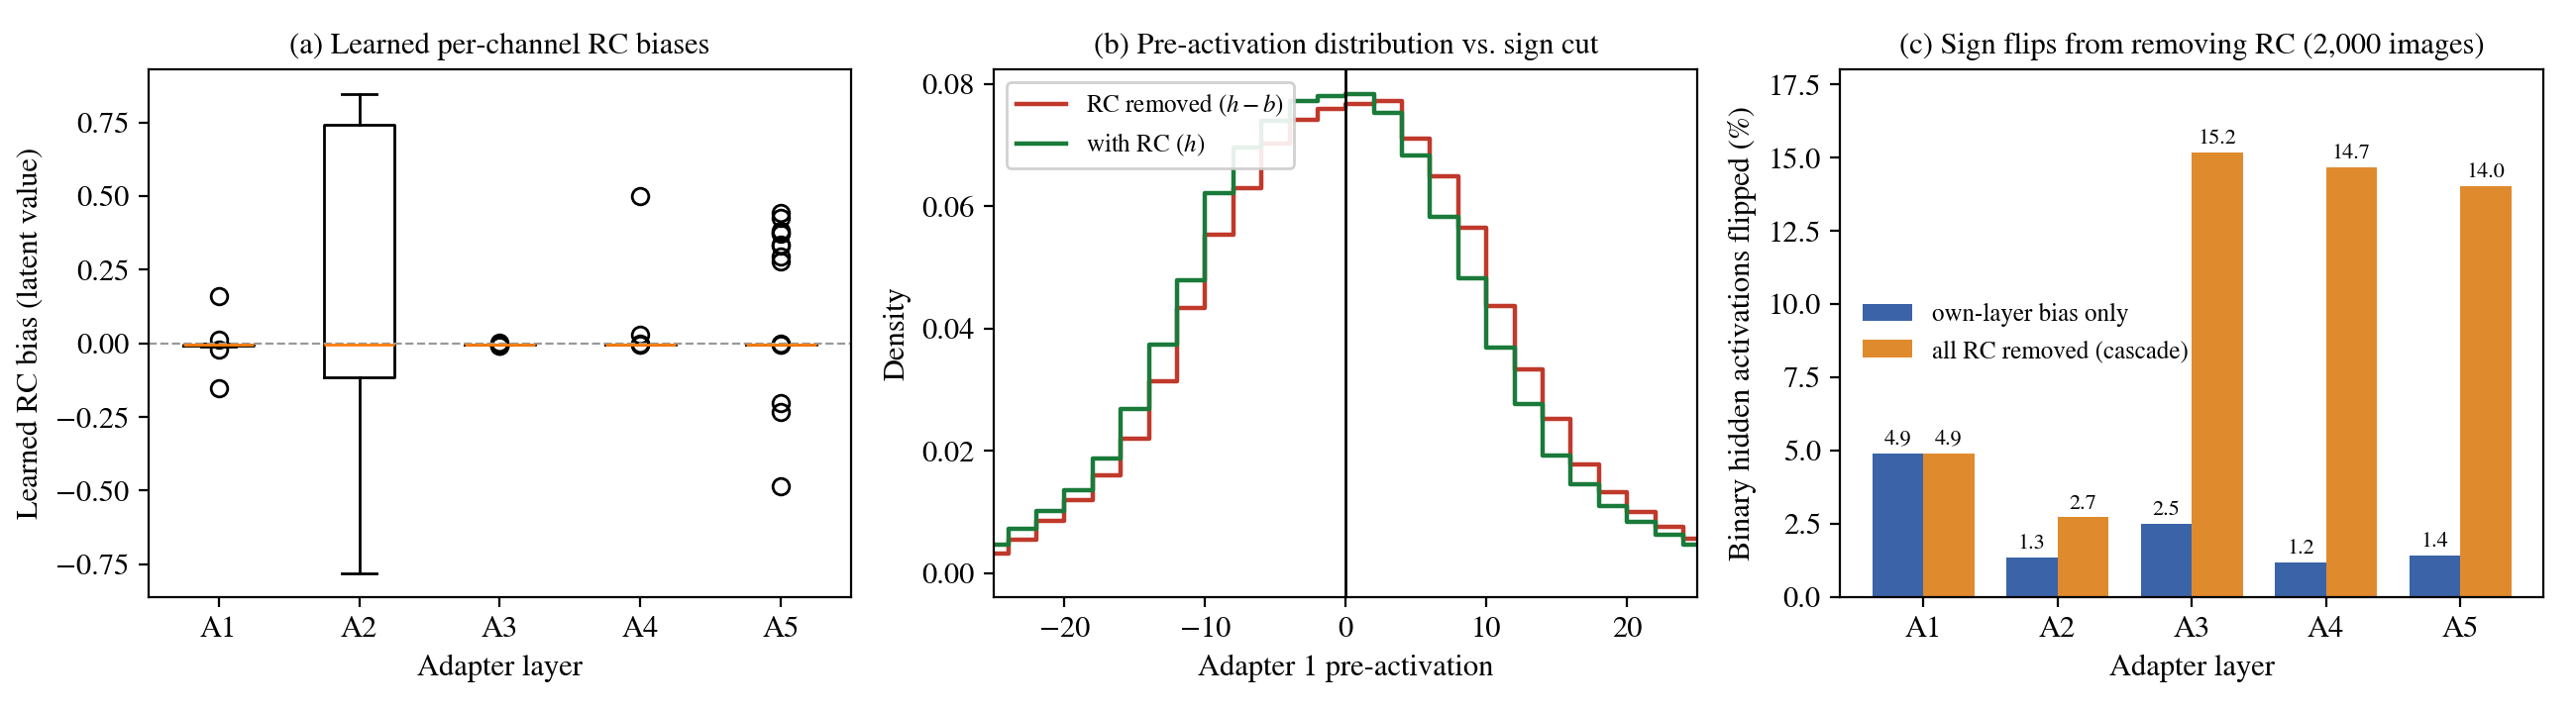
\includegraphics[width=\linewidth,keepaspectratio]{rc_mechanism.png}
\caption{Mechanism-Level Probe of RC on a Deployed-Geometry CIFAR-10$\to$SVHN Checkpoint (2,000 Test Images).}
\label{fig:rc_mechanism}
\end{figure}

To complement the ablation with mechanism-level evidence, Figure~\ref{fig:rc_mechanism} probes a trained deployed-geometry $M{=}1$ checkpoint (seed 2024) directly. Panel~(a) shows the learned per-channel RC biases: nonzero values of both signs with layer-dependent spread. Panel~(b) pools the down-projection pre-activations of Adapter~1 over 2,000 SVHN test images: a substantial fraction of the mass lies close to the sign cut, so even sub-unit shifts of the cut change binary decisions. Panel~(c) quantifies this: zeroing a single layer's RC flips $1.2$--$4.9\%$ of that layer's binary hidden activations, and removing RC everywhere compounds through the frozen binary backbone to alter $14$--$15\%$ of the binary codes at the deeper adapters. These observations are consistent with the hypothesis that RC's role is to position the binarisation cut rather than to add representational capacity, although they do not by themselves isolate the causal pathway from cut position to final accuracy.

\begin{table}[H]
\centering
\caption{Multi-Branch Adapter Scaling Contribution of MARS Across Four Targets.}
\label{tab:multi_adapter_contrib}
\begin{tabular}{lrrrrrr}
\toprule
 & \multicolumn{4}{c}{\textbf{MARS}} & & \\
\cmidrule(lr){2-5}
\textbf{Target} & \textbf{$M{=}1$} & \textbf{$M{=}2$} & \textbf{$M{=}3$} & \textbf{$M{=}4$} & \textbf{$\Delta_{\text{multi}}$ (pp)} & \textbf{Full-FT} \\
\midrule
SVHN         & 73.72\% & 77.16\% & 78.77\% & \textbf{79.81\%} & +6.09 & 94.91\% \\
FashionMNIST & 80.42\% & 82.00\% & 82.82\% & \textbf{83.54\%} & +3.12 & 92.36\% \\
STL10        & 67.46\% & 67.58\% & 68.00\% & \textbf{68.06\%} & +0.60 & 71.05\% \\
CINIC10      & 64.80\% & 65.16\% & 65.38\% & \textbf{65.45\%} & +0.65 & 68.02\% \\
\bottomrule
\end{tabular}
\end{table}

Table~\ref{tab:multi_adapter_contrib} re-presents the same MARS data organised by branch count, isolating the multi-branch gain $\Delta_{\text{multi}}$ over the single-branch baseline for each target.

\section{FPGA Resource Utilization and Power}
\label{sec:hw_results}

\subsection{Cross-Configuration Resource Comparison}
\label{sec:resource_compare}

Table~\ref{tab:resource_compare} compares the post-implementation FPGA resource utilisation across four build configurations of the same MARS architecture on XC7Z020. Two axes are varied: \emph{throughput} vs.\ \emph{compactness} folding of the integrated MVAU + Adapter datapath (Section~\ref{sec:pe_simd_breakdown}), and \emph{absence} vs.\ \emph{presence} of the cfg\_hub runtime-switching infrastructure (Section~\ref{sec:runtime_switch}). The first row is the FINN-generated throughput backbone alone (no adapter, no cfg\_hub), the throughput resource zero-baseline; the second is the throughput build with the Adapter IP and cfg\_hub integrated (2-task); the third is the compactness (PE = 1) backbone alone, the compactness zero-baseline; and the fourth is the genuine deployed compactness build that hosts runtime cfg-switching for five task models (Section~\ref{sec:pe1_3ds}).

\begin{table}[H]
\centering
\caption{FPGA Resource Utilisation Across Four MARS Build Configurations.}
\label{tab:resource_compare}
\renewcommand{\arraystretch}{1.2}%
\resizebox{\linewidth}{!}{%
\begin{tabular}{lc rrrr}
\toprule
\textbf{Configuration} & \textbf{Function Switch} & \textbf{Occupied Slices} & \textbf{Slice LUTs} & \textbf{Slice Reg.\ (FF)} & \textbf{BRAM} \\
\midrule
Backbone (Throughput)     & no & 11{,}648 (87.58\%) & 25{,}322 (47.60\%) & 31{,}621 (29.72\%) & 99.5 (71.07\%) \\
MARS (Throughput, 2-task)         & yes & 13{,}272 (99.79\%) & 41{,}729 (78.44\%) & 53{,}285 (50.08\%) & 99\hphantom{.0} (70.71\%) \\
Backbone (Compactness) & no & 8{,}926 (67.11\%) & 15{,}651 (29.42\%) & 22{,}219 (20.88\%) & 85\hphantom{.0} (60.71\%) \\
MARS (Compactness, N-task)     & yes & 12{,}957 (97.42\%) & 39{,}967 (75.13\%) & 40{,}926 (38.46\%) & 84\hphantom{.0} (60.00\%) \\
\bottomrule
\end{tabular}%
}
\begin{flushleft}
\footnotesize On XC7Z020 each slice holds 4 LUTs and 8 flip-flops, and a slice is counted as \emph{occupied} as soon as any single one of them is used; occupied-slice utilisation can therefore far exceed the Slice-LUT or FF utilisation when distributed-RAM (LUTRAM) logic and control-set constraints spread the design across the placement grid---reducing the LUT count does not free slices unless the remaining logic can be packed more densely. Integrating the adapter (with cfg\_hub) drives slice occupancy to near-saturation despite sub-80\% LUT use---the distributed-RAM-dominated Adapter IP structure saturates the placement grid: the throughput build reaches 13{,}272 / 13{,}300 (99.79\%), and the genuinely deployed compactness build reaches 12{,}957 / 13{,}300 (97.42\%). The cfg\_hub itself costs only 19 LUTs, adding negligible resources over the bare adapter integration. The compactness backbone alone (no adapter) is only 15{,}651 LUT / 8{,}926 slices: uniform PE = 1 folding frees the slice headroom that is then reinvested into hosting one fully runtime-writable active-task state, into which host-resident task images are loaded sequentially (Section~\ref{sec:pe1_3ds}).
\end{flushleft}
\end{table}

Key observations:
\begin{itemize}
    \item \textbf{Zero DSP overhead}: Both configurations use zero DSP slices, confirming that all arithmetic (XNOR, popcount, LUT-based contribution scaling) is implemented in combinational logic.
    \item \textbf{BRAM parity}: Adding the adapter does not increase BRAM usage ($-0.5$ tiles). This is the direct consequence of implementing all adapter down-/up-projection weights and contribution LUTs in distributed RAM (LUT-RAM), keeping BRAM reserved for the backbone memstream banks.
    \item \textbf{LUT usage}: The deployed compactness build uses 39{,}967 LUTs (75.13\%). Post-route hierarchical analysis attributes roughly 25{,}593 LUTs ($\sim$48\% of the chip) to the five adapter-hosting Super Wrappers combined, dominated by the adapter datapath (weight RAMs and XNOR-popcount trees) and the threshold-comparison logic.
    \item \textbf{Slice saturation}: The 97.42\% slice utilisation of the deployed compactness build (99.79\% on the throughput build) means that any further additions must be accompanied by logic-level optimisation to free slice sites rather than merely LUTs. This is the primary constraint for scaling the Adapter IP to $M{\geq}2$ configurations on XC7Z020 without a larger platform.
\end{itemize}

Figure~\ref{fig:soc_layout} shows the post-implementation placement of the MARS compactness build on the XC7Z020 fabric, coloured by functional group; the colour legend is shown beside the figure. The placement makes the utilisation figures above directly visible: adapter logic (yellow) and backbone MVAUs (green) dominate the occupied area and interleave across the die, whereas the Function Switch Controller (purple) appears only as a negligible scattering of cells, matching its 19-LUT footprint.

\begin{figure}[H]
\centering
\begin{minipage}[c]{0.55\linewidth}
\centering
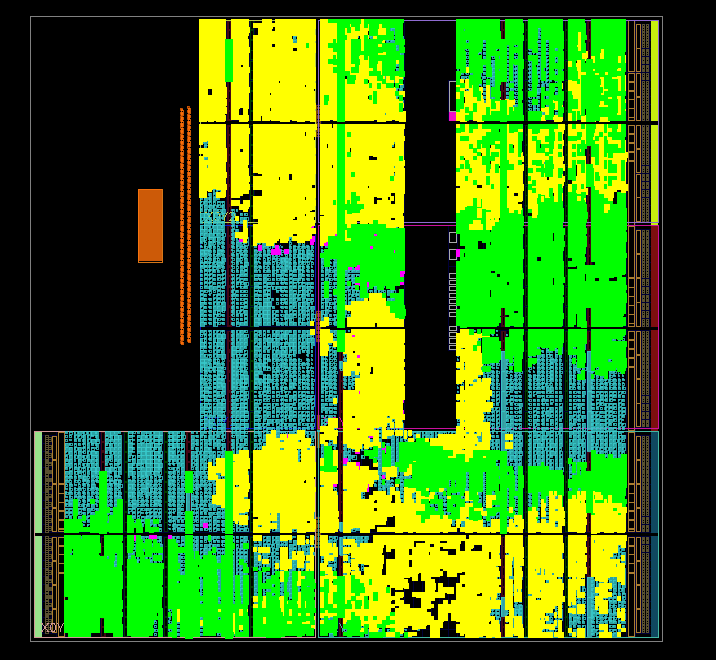
\includegraphics[width=\linewidth,keepaspectratio]{mars_soc_layout.png}
\end{minipage}\hfill
\begin{minipage}[c]{0.4\linewidth}
\small
\renewcommand{\arraystretch}{1.7}%
\begin{tabular}{@{}c@{\ \ }l@{}}
\fcolorbox{black}{layYellow}{\rule{0pt}{8pt}\rule{16pt}{0pt}} & Adapter + Adapter RAM \\
\fcolorbox{black}{layGreen}{\rule{0pt}{8pt}\rule{16pt}{0pt}} & MVAU \\
\fcolorbox{black}{layPurple}{\rule{0pt}{8pt}\rule{16pt}{0pt}} & Function Switch Controller \\
\fcolorbox{black}{layOrange}{\rule{0pt}{8pt}\rule{16pt}{0pt}} & PS (processing system) \\
\fcolorbox{black}{layBlue}{\rule{0pt}{8pt}\rule{16pt}{0pt}} & Other SoC logic \\
\end{tabular}
\end{minipage}
\caption{Post-implementation layout of the MARS compactness build on XC7Z020.}
\label{fig:soc_layout}
\end{figure}

\subsection{Power Consumption}

\begin{table}[H]
\centering
\caption{Power Across the Four MARS Build Configurations.}
\label{tab:power}
\begin{tabular}{lrrr}
\toprule
\textbf{Build} & \textbf{Total (W)} & \textbf{Dynamic (W)} & \textbf{Static (W)} \\
\midrule
Backbone (Throughput)     & 2.114 & 1.949 & 0.165 \\
MARS (Throughput, 2-task)         & 2.215 & 2.046 & 0.168 \\
Backbone (Compactness) & 1.782 & 1.629 & 0.152 \\
MARS (Compactness, N-task)     & 1.802 & 1.649 & 0.153 \\
\bottomrule
\end{tabular}
\end{table}

On the throughput build, integrating the adapter together with the cfg\_hub raises total on-chip power by only 0.101~W ($+4.8\%$; 2.114~$\to$~2.215~W), with the dynamic term rising from 1.949~W to 2.046~W; the runtime-switching cfg\_hub itself adds negligible power. (The adapter-enabled throughput build without cfg\_hub measures 2.214~W, the figure used for the energy-efficiency comparison in Section~\ref{sec:cross_platform}.) Decomposing the PL side of the adapter-enabled throughput build, the streaming dataflow (StreamingDataflowPartition\_1, the user logic) consumes only 0.732~W, while the ARM PS sub-system contributes 1.256~W---most of the residual is the always-on PS. The compactness builds draw less total power (1.78--1.80~W) because uniform PE = 1 folding instantiates far less parallel logic. In practical terms, the user-facing inference pipeline remains sub-watt, which is the relevant figure for edge deployment. The cross-platform comparison below reports total FPGA on-chip power to match the broad device-level power accounting used for the GPU/Jetson measurements as closely as available; the methodology nonetheless remains asymmetric, because the FPGA figure is Vivado-estimated whereas the GPU/Jetson figures are runtime-measured. All throughput and energy-efficiency figures in this section pertain to the throughput build (heterogeneous PE up to 32); the compactness design point introduced for $N$-task runtime switching (Section~\ref{sec:pe1_3ds}) deliberately time-folds the convolution datapath and runs at $\approx$107~img/s, so the throughput build remains the configuration of record for the efficiency comparison.

\subsection{Per-Layer PE Configuration: Throughput vs Compactness}
\label{sec:pe_simd_breakdown}

Table~\ref{tab:pe_simd_config} compares the per-layer PE folding factors of the throughput build against the compactness build of the same integrated MVAU + Adapter datapath. The throughput build selects substantially higher PE factors for the convolution layers (Conv1--Conv5) to unfold the integrated datapath and sustain the streaming throughput reported above; the compactness build (used for the runtime task switching demonstration in Section~\ref{sec:pe1_3ds}) uses uniform PE = 1 across all convolutional units (MVAU0 and Super1--5) and reinvests the resulting slice/LUT headroom in the cfg-writable adapter and threshold storage. The fully-connected units MVAU6--MVAU8 host no adapter and therefore retain their original folding in both builds.



\begin{table}[H]
\centering
\caption{Per-Layer PE Folding for the Throughput and Compactness Builds.}
\label{tab:pe_simd_config}
\begin{tabular}{ccc}
\toprule
\textbf{Layer} & \textbf{Throughput PE} & \textbf{Compactness PE} \\
\midrule
MVAU0 & 16 & 1 \\
Super1 & 32 & 1 \\
Super2 & 16 & 1 \\
Super3 & 16 & 1 \\
Super4 & 4  & 1 \\
Super5 & 1  & 1 \\
MVAU6 & 1  & 1 \\
MVAU7 & 1  & 1 \\
MVAU8 & 5  & 5 \\
\bottomrule
\end{tabular}
\end{table}

\begin{figure}[H]
\centering
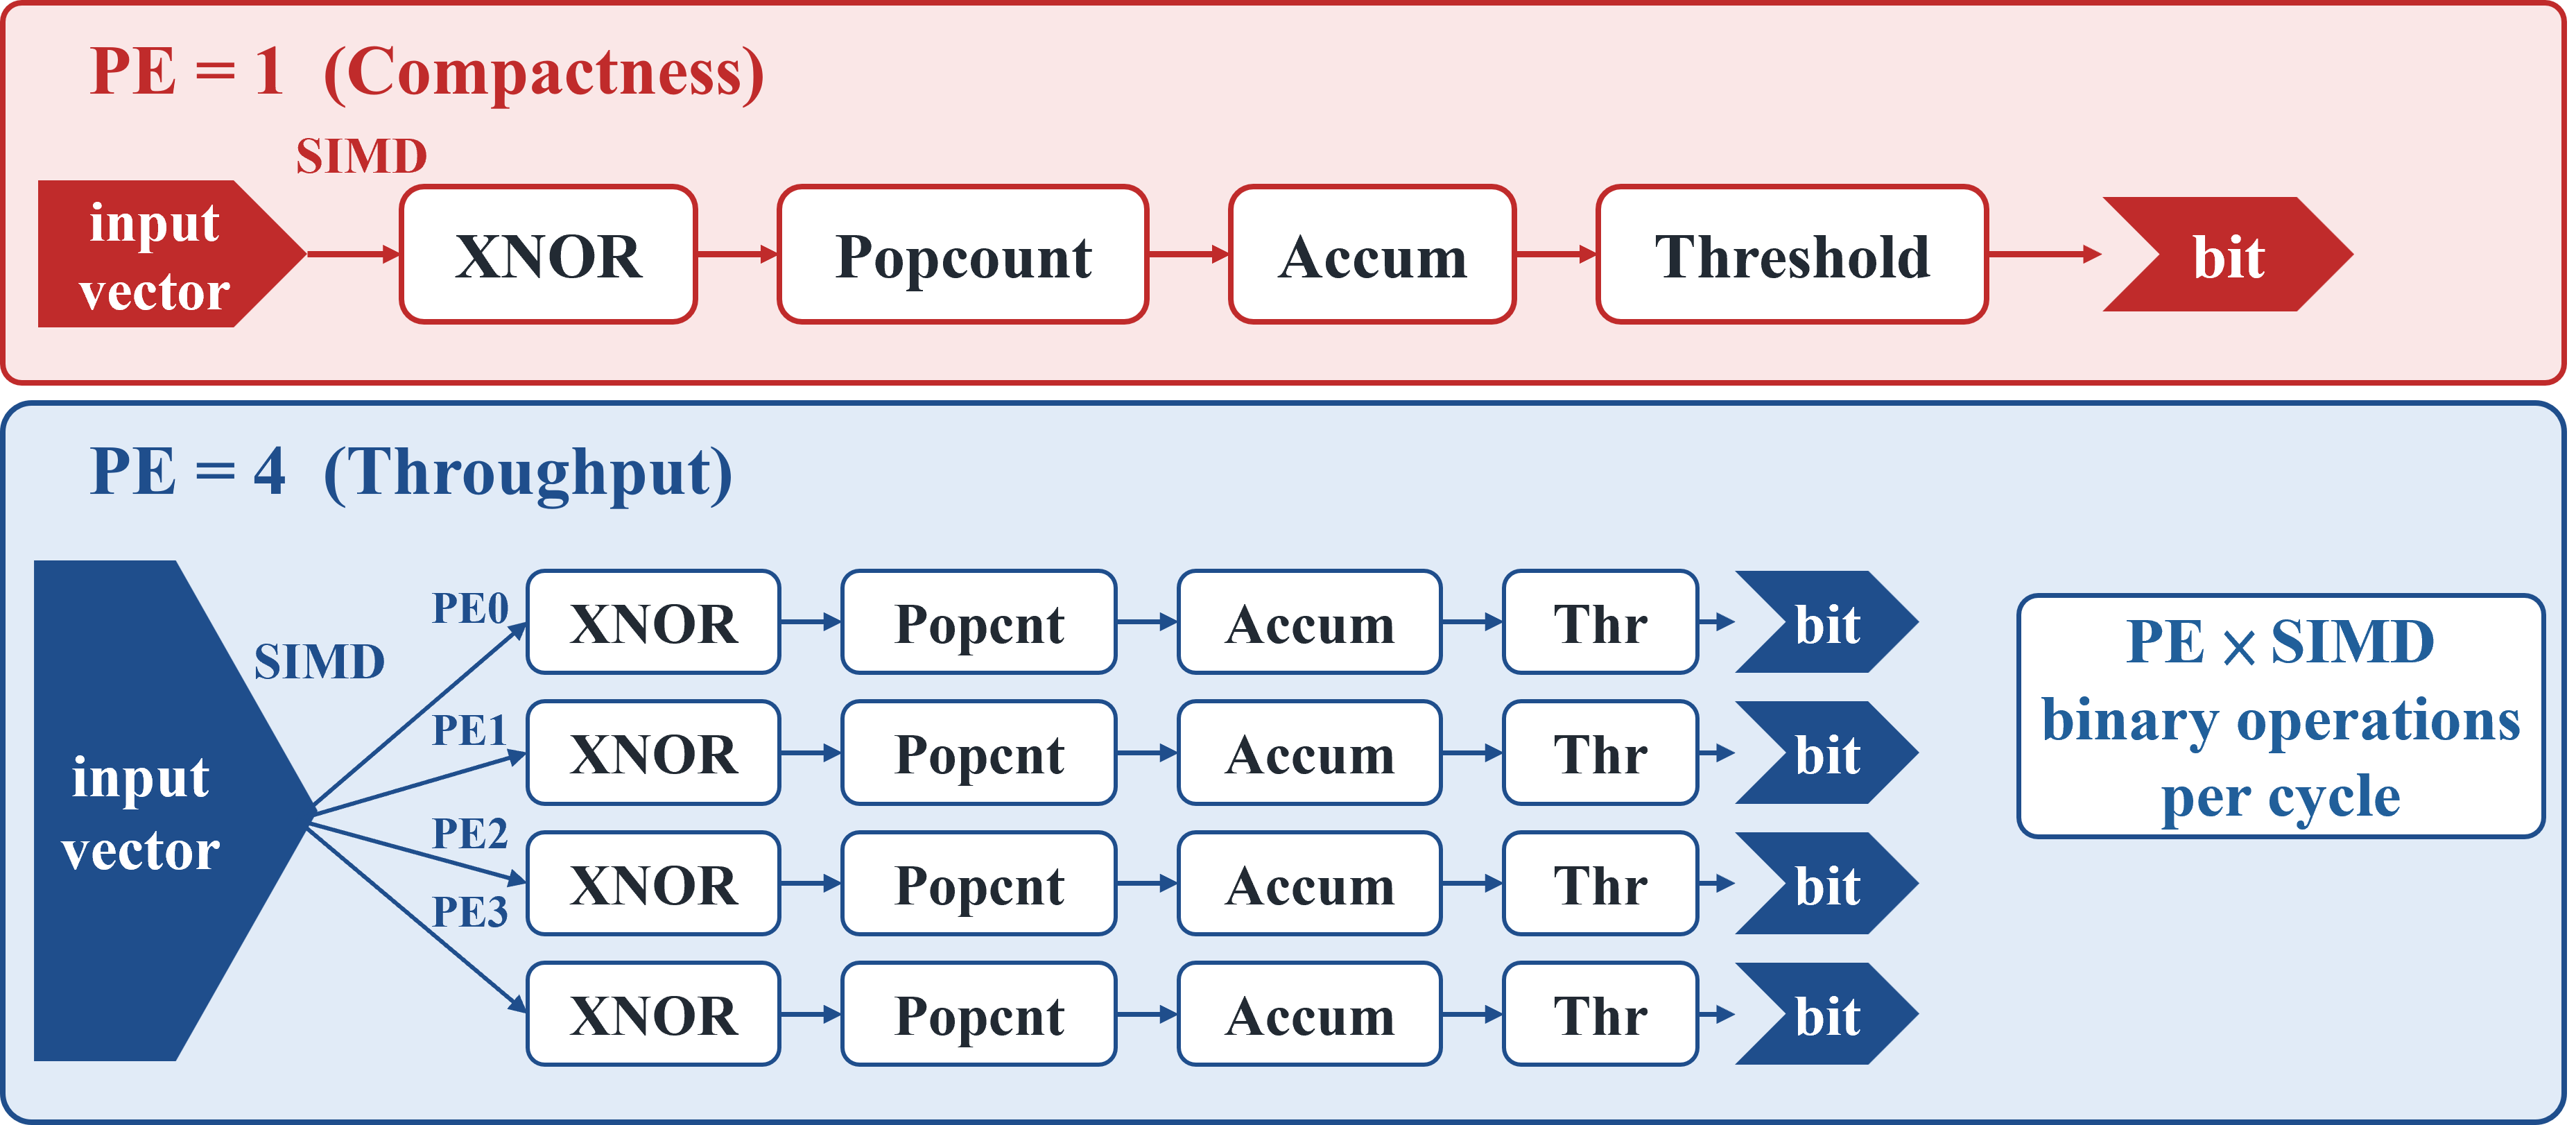
\includegraphics[width=\linewidth,keepaspectratio]{pe_diff.png}
\caption[PE Folding of the Throughput and Compactness Builds]{Folding Difference between the Two Builds: PE${=}1$ (Compactness) vs.\ PE-Parallel Lanes (Throughput, Illustrated for PE${=}4$).}
\label{fig:pe_diff}
\end{figure}

Figure~\ref{fig:pe_diff} visualises this folding difference. With uniform PE${=}1$ (compactness), each convolutional unit instantiates a single XNOR--popcount--accumulate--threshold lane that computes the output channels serially, minimising logic and freeing the slice headroom that is reinvested into the cfg-writable per-task state. The throughput build instead instantiates PE parallel lanes per unit (illustrated for PE${=}4$; the actual per-layer factors reach 32, Table~\ref{tab:pe_simd_config}), each with its own accumulator and threshold comparator, so a unit completes PE$\times$SIMD binary operations per cycle. The two builds share identical lane RTL; only the number of instantiated lanes differs; this PE-folding difference is the dominant architectural source of the $\approx$17.4$\times$ throughput gap and of the complementary slice headroom analysed above.


\subsection{Multi-Branch Scaling Cost and Accuracy--Resource Trade-Off}
\label{sec:multibranch_cost}

Chapter~\ref{ch:methodology} predicts a linear parameter growth for Multi-Branch Adapter scaling; this subsection verifies the prediction directly in hardware. The $M{=}2$--$4$ variants of both build styles are implemented in RTL and carried through the same FINN Zynq flow as the deployed accelerator: each adapter site's Super Wrapper instantiates $M$ parallel copies of the unchanged Adapter datapath, whose Q8 contributions are summed before the shared threshold compare (the hardware realisation of Eq.~(\ref{eq:multi_adapter})); the five per-site IPs are re-packaged, the streaming partition is re-exported, and the identical Zynq top-level design---PS, DMA engines, and interconnect untouched---is synthesised with the same strategy as the deployed builds. Every variant is first verified by the same per-MVAU RTL simulation protocol as the deployed design: for all five sites and all $M \in \{1,\dots,4\}$ in both build styles, the RTL output is bit-exact against the integer golden model loaded with the real trained deployed-geometry branch weights (40/40 simulations pass). Because the $M \geq 2$ designs exceed the XC7Z020 capacity, place-and-route cannot complete; all scaling numbers in Table~\ref{tab:multibranch_scaling} are therefore reported at the synthesis stage, for all $M$ including $M{=}1$, so that every comparison is made at the same stage of the flow.

\begin{table}[H]
\centering
\caption{Post-Synthesis Resource and Power Scaling of Multi-Branch MARS on XC7Z020.}
\label{tab:multibranch_scaling}
\small
\renewcommand{\arraystretch}{1.2}%
\setlength{\tabcolsep}{4.5pt}%
\begin{tabular}{clrrcc}
\toprule
\textbf{Build} & \textbf{$M$} & \textbf{Slice LUTs} & \textbf{Slice Reg.\ (FF)} & \textbf{BRAM} & \textbf{Power (W)} \\
\midrule
\multirow{4}{*}{Throughput (2-task)}
 & 1 & 73{,}169 (137.5\%)  & 65{,}717 (61.8\%)   & 99 & 2.135 \\
 & 2 & 109{,}731 (206.3\%) & 86{,}727 (81.5\%)   & 99 & 2.193 \\
 & 3 & 145{,}061 (272.7\%) & 107{,}471 (101.0\%) & 99 & 2.337 \\
 & 4 & 187{,}521 (352.5\%) & 128{,}698 (121.0\%) & 99 & 2.468 \\
\midrule
\multirow{4}{*}{Compactness (N-task)}
 & 1 & 47{,}931 (90.1\%)   & 42{,}922 (40.3\%)   & 84 & 1.841 \\
 & 2 & 71{,}841 (135.0\%)  & 60{,}390 (56.8\%)   & 84 & 1.897 \\
 & 3 & 95{,}593 (179.7\%)  & 77{,}830 (73.2\%)   & 84 & 1.915 \\
 & 4 & 125{,}538 (236.0\%) & 95{,}285 (89.6\%)   & 84 & 1.969 \\
\bottomrule
\end{tabular}
\begin{flushleft}
\footnotesize All builds use zero DSP slices and a constant BRAM count: every added branch is realised entirely in LUT/FF logic and distributed RAM, so the memstream banks are unaffected. Percentages are relative to the XC7Z020 (53{,}200 LUTs, 106{,}400 FFs). Power is the Vivado vectorless estimate on the post-synthesis Zynq-top netlist (PS included) at 100~MHz.
\end{flushleft}
\end{table}

Table~\ref{tab:mb_cost} restates the per-$M$ cost of the compactness build together with the parameter overhead, so that the linear-cost claim of Section~\ref{sec:multi_adapter} is supported by synthesis-reported resource values and vectorless power estimates.

\begin{table}[H]
\centering
\caption{Per-Branch Parameter and Post-Synthesis Cost of the Compactness Build.}
\label{tab:mb_cost}
\resizebox{\linewidth}{!}{%
\begin{tabular}{ccccc}
\toprule
\textbf{M} & \textbf{Added Params} & \textbf{Vs.\ Backbone (1{,}546{,}690)} & \textbf{Slice LUTs (\% XC7Z020)} & \textbf{Power (W)} \\
\midrule
1 & 58{,}533  & $+3.78\%$  & 47{,}931 (90.1\%)   & 1.841 \\
2 & 117{,}066 & $+7.57\%$  & 71{,}841 (135.0\%)  & 1.897 \\
3 & 175{,}599 & $+11.35\%$ & 95{,}593 (179.7\%)  & 1.915 \\
4 & 234{,}132 & $+15.14\%$ & 125{,}538 (236.0\%) & 1.969 \\
\bottomrule
\end{tabular}%
}
\end{table}

Three observations follow. First, resource growth is linear and predictable, as claimed in Section~\ref{sec:multi_adapter}: each added branch costs $+23.8$k--$29.9$k LUTs on the compactness build and $+35.3$k--$42.5$k LUTs on the throughput build, with BRAM constant and zero DSPs throughout. Second, the XC7Z020 is exhausted immediately: already at $M{=}2$ the LUT demand alone reaches $135\%$ (compactness) and $206\%$ (throughput) of the device, so no amount of placement effort can close the gap---multi-branch deployment requires a larger part, quantifying the constraint anticipated in Section~\ref{sec:resource_compare}. Third, power is not the binding constraint: from $M{=}1$ to $M{=}4$ the estimated total power rises by only $0.13$~W ($+7.0\%$) on the compactness build, because the always-on PS and the backbone dominate; the trade-off is area-bound.

Synthesis-stage figures overstate the final cost, because placement and physical optimisation prune and re-pack logic across module boundaries. Table~\ref{tab:synth_vs_impl} calibrates this effect on the $M{=}1$ builds, where implementation completes and the published post-implementation numbers of Tables~\ref{tab:resource_compare} and~\ref{tab:power} are available: place-and-route recovers $16.6\%$ of the synthesis-stage LUTs on the compactness build and $43.0\%$ on the throughput build (whose PE-parallel adapter storage offers more re-packing opportunity). The synthesis-stage scaling numbers above are therefore conservative upper bounds---and even under this optimistic reading every $M \geq 2$ configuration remains beyond the device: still beyond on the compactness build ($\approx 113\%$ LUT at $M{=}2$ after the same recovery) and far beyond on the throughput build.

\begin{table}[H]
\centering
\caption{Synthesis vs.\ Implementation Utilisation of the $M{=}1$ Builds.}
\label{tab:synth_vs_impl}
\small
\renewcommand{\arraystretch}{1.2}%
\setlength{\tabcolsep}{4.5pt}%
\begin{tabular}{clrrc}
\toprule
\textbf{Build} & \textbf{Stage} & \textbf{Slice LUTs} & \textbf{Slice Reg.\ (FF)} & \textbf{Power (W)} \\
\midrule
\multirow{2}{*}{Throughput (2-task)}
 & synthesis            & 73{,}169 (137.5\%) & 65{,}717 & 2.135 \\
 & implementation       & 41{,}729 (78.4\%)  & 53{,}285 & 2.215 \\
\midrule
\multirow{2}{*}{Compactness (N-task)}
 & synthesis            & 47{,}931 (90.1\%)  & 42{,}922 & 1.841 \\
 & implementation       & 39{,}967 (75.1\%)  & 40{,}926 & 1.802 \\
\bottomrule
\end{tabular}
\begin{flushleft}
\footnotesize Implementation rows are the published post-implementation builds of Tables~\ref{tab:resource_compare} and~\ref{tab:power} (occupied slices 13{,}272 / 12{,}957, i.e.\ 99.8\% / 97.4\%). Occupied-slice counts exist only after placement and are therefore undefined for the synthesis-stage rows.
\end{flushleft}
\end{table}

The accuracy side of the trade-off is quantified on twenty deployed-geometry transfer pairs: every combination of five backbones (CIFAR-10, SVHN, STL10, FashionMNIST, CINIC10) and four target datasets, each trained at $M{=}1$--$4$ with RC under the identical protocol as Section~\ref{sec:sw_results}. Table~\ref{tab:multibranch_acc16} lists all twenty pairs; the CIFAR-10-backbone rows repeat Table~\ref{tab:multi_adapter_contrib}, and the remaining sixteen pairs are newly trained for this study. Unlike the cross-backbone study of Table~\ref{tab:multi_adapter_backbones}, which uses the wide software geometry, every number here uses the deployed geometry that the hardware cost of Table~\ref{tab:multibranch_scaling} corresponds to. All adapter branches are cfg-writable, while the fixed-size backbone memories are unchanged across tasks; the hardware cost is therefore identical for every pair, and all twenty accuracy trajectories share the same hardware-cost axis.

\begin{table}[p]
\centering
\caption{Deployed-Geometry Multi-Branch Transfer Accuracy over 20 Backbone--Target Pairs.}
\label{tab:multibranch_acc16}
\renewcommand{\arraystretch}{1.0}%
\begin{tabular}{llrrrrr}
\toprule
\textbf{Backbone} & \textbf{Target} & \textbf{$M{=}1$} & \textbf{$M{=}2$} & \textbf{$M{=}3$} & \textbf{$M{=}4$} & \textbf{$\Delta_{\text{multi}}$ (pp)} \\
\midrule
\multirow{4}{*}{CIFAR-10} & SVHN & 73.72\% & 77.16\% & 78.77\% & 79.81\% & +6.09 \\
 & FashionMNIST & 80.42\% & 82.00\% & 82.82\% & 83.54\% & +3.12 \\
 & STL10 & 67.46\% & 67.58\% & 68.00\% & 68.06\% & +0.60 \\
 & CINIC10 & 64.80\% & 65.16\% & 65.38\% & 65.45\% & +0.65 \\
\midrule
\multirow{4}{*}{SVHN} & CIFAR-10 & 43.18\% & 45.13\% & 46.93\% & 48.37\% & +5.19 \\
 & FashionMNIST & 78.51\% & 79.76\% & 80.56\% & 81.89\% & +3.38 \\
 & STL10 & 34.41\% & 34.60\% & 35.45\% & 35.10\% & +0.69 \\
 & CINIC10 & 33.59\% & 35.21\% & 34.29\% & 38.03\% & +4.44 \\
\midrule
\multirow{4}{*}{STL10} & CIFAR-10 & 66.65\% & 67.90\% & 68.74\% & 68.79\% & +2.14 \\
 & FashionMNIST & 81.48\% & 82.96\% & 83.58\% & 84.19\% & +2.71 \\
 & SVHN & 68.15\% & 73.18\% & 74.17\% & 75.65\% & +7.50 \\
 & CINIC10 & 54.26\% & 55.33\% & 56.17\% & 56.56\% & +2.30 \\
\midrule
\multirow{4}{*}{FashionMNIST} & CIFAR-10 & 33.63\% & 34.67\% & 35.84\% & 36.76\% & +3.13 \\
 & STL10 & 32.64\% & 32.29\% & 33.64\% & 34.11\% & +1.47 \\
 & SVHN & 51.37\% & 58.19\% & 59.42\% & 62.70\% & +11.33 \\
 & CINIC10 & 27.75\% & 28.37\% & 29.55\% & 29.56\% & +1.81 \\
\midrule
\multirow{4}{*}{CINIC10} & CIFAR-10 & 78.21\% & 78.60\% & 78.87\% & 78.72\% & +0.51 \\
 & SVHN & 69.14\% & 73.88\% & 75.39\% & 76.34\% & +7.20 \\
 & STL10 & 67.21\% & 67.60\% & 67.54\% & 67.42\% & +0.21 \\
 & FashionMNIST & 80.23\% & 81.86\% & 82.17\% & 82.88\% & +2.65 \\
\midrule
\multicolumn{2}{l}{\textbf{Mean gain over $M{=}1$ (pp)}} & --- & +1.73 & +2.52 & +3.36 & --- \\
\bottomrule
\end{tabular}
\begin{flushleft}
\footnotesize All entries use the FPGA-deployed adapter geometry with RC ($\Delta_{\text{multi}} = M{=}4 - M{=}1$); the CIFAR-10 rows are those of Table~\ref{tab:multi_adapter_contrib}, and the other sixteen pairs follow the same 200-epoch protocol. Table~\ref{tab:multi_adapter_backbones} uses the wide software geometry; the two tables are not cell-by-cell comparable, and the geometry ranking itself is source-dependent (see the scope note in Section~\ref{sec:backbone_effect}). All twenty pairs are single-seed (2024); representative $n{=}5$ paired tests are reported for CIFAR-10$\to$SVHN and CIFAR-10$\to$FashionMNIST (Section~\ref{sec:rc_multiseed}).
\end{flushleft}
\end{table}

\begin{figure}[H]
\centering
\begin{minipage}{0.49\linewidth}\centering
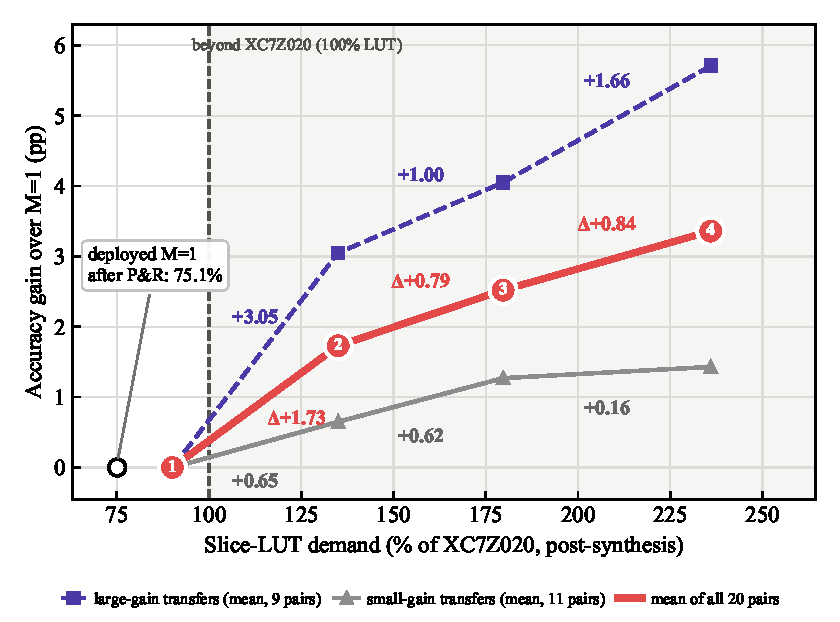
\includegraphics[width=\linewidth,keepaspectratio]{mb_tradeoff_compact_lut.pdf}\\[-1pt]
{\footnotesize (a) Compactness (N-task)}
\end{minipage}\hfill
\begin{minipage}{0.49\linewidth}\centering
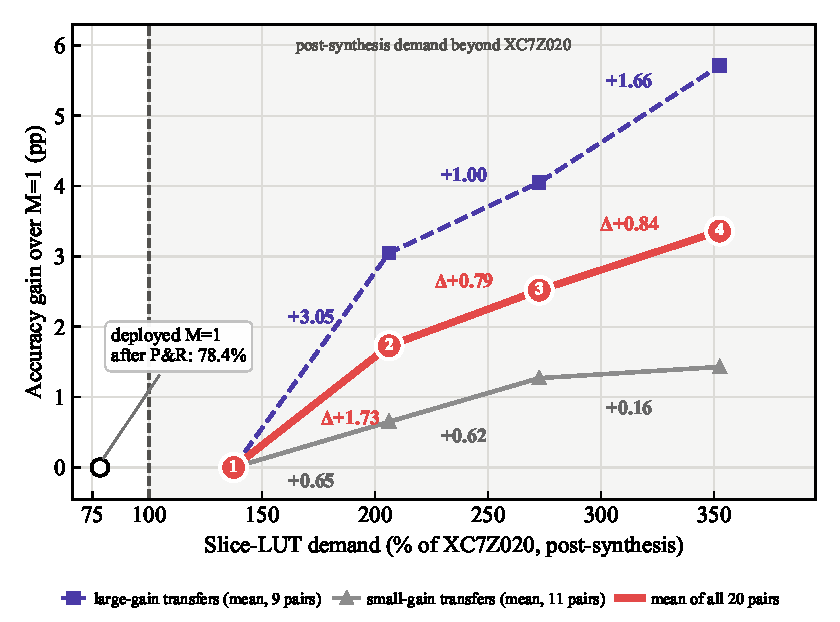
\includegraphics[width=\linewidth,keepaspectratio]{mb_tradeoff_throughput_lut.pdf}\\[-1pt]
{\footnotesize (b) Throughput (2-task)}
\end{minipage}
\caption[Accuracy Gain vs.\ Post-Synthesis LUT Demand (20 Pairs)]{Accuracy Gain Versus Post-Synthesis LUT Demand for Multi-Branch Scaling (20 Pairs). Large-Gain Transfers: $\Delta_{\text{multi}} = \mathrm{Acc}_{M=4}-\mathrm{Acc}_{M=1} \geq 3$~pp (9 Pairs); the Remaining 11 Pairs Form the Small-Gain Group.}
\label{fig:multibranch_tradeoff}
\end{figure}

\begin{figure}[H]
\centering
\begin{minipage}{0.49\linewidth}\centering
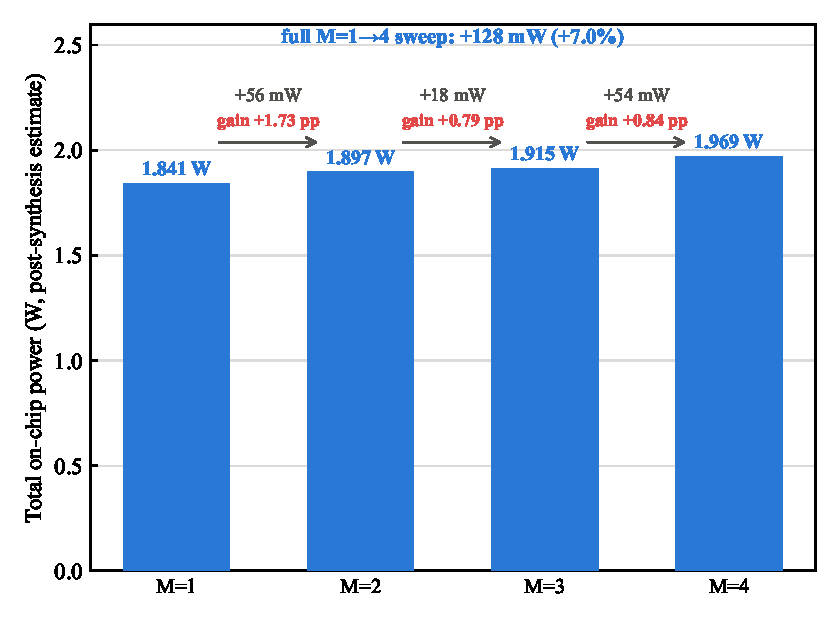
\includegraphics[width=\linewidth,keepaspectratio]{mb_tradeoff_compact_power.pdf}\\[-1pt]
{\footnotesize (a) Compactness (N-task)}
\end{minipage}\hfill
\begin{minipage}{0.49\linewidth}\centering
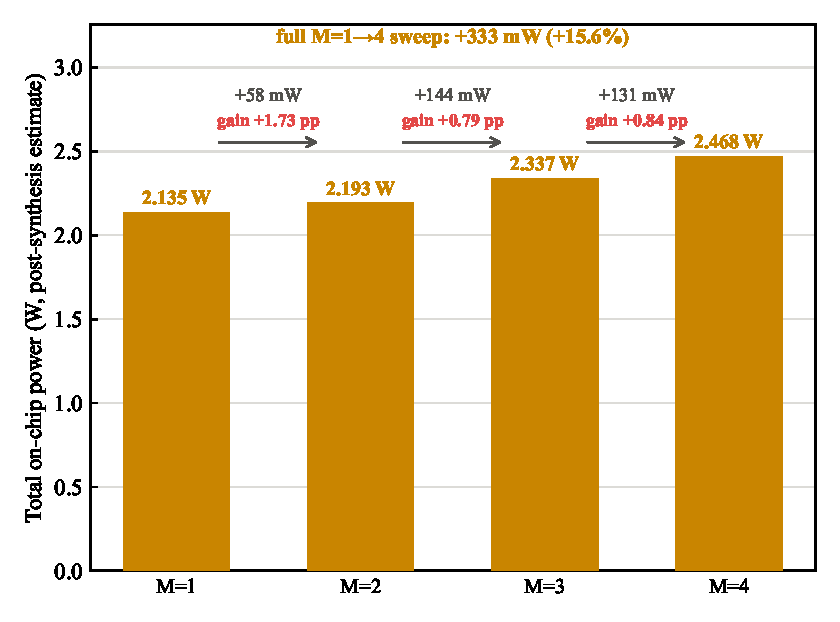
\includegraphics[width=\linewidth,keepaspectratio]{mb_tradeoff_throughput_power.pdf}\\[-1pt]
{\footnotesize (b) Throughput (2-task)}
\end{minipage}
\caption{Total On-Chip Power Across Branch Counts (Post-Synthesis Estimates).}
\label{fig:multibranch_power}
\end{figure}

Figures~\ref{fig:multibranch_tradeoff} and~\ref{fig:multibranch_power} expose the resulting trade-off, and the numbers make the cost-performance ranking explicit. Each panel of Figure~\ref{fig:multibranch_tradeoff} shows the mean over all twenty pairs (bold) together with the means of the nine large-gain ($\Delta_{\text{multi}} \geq 3$~pp) and the eleven small-gain transfers, and its cost axis is the \emph{post-synthesis} demand of Table~\ref{tab:multibranch_scaling}, which overstates the final footprint: the deployed $M{=}1$ builds fit on the device after place-and-route ($75.1\%$/$78.4\%$ LUT, hollow markers; Table~\ref{tab:synth_vs_impl}), so the shaded infeasible region concerns the $M \geq 2$ points. Averaged over the twenty pairs, the first added branch is worth $+1.73$~pp, while the second and third are worth only $+0.79$ and $+0.84$~pp---yet every added branch costs a near-identical $+23.8$k--$29.9$k LUTs on the compactness build. In cost-performance terms the first step returns $0.72$~pp per $10$k LUTs, more than double the $0.33$/$0.28$~pp of the later steps: $M{=}2$ is where the accuracy return per unit of hardware peaks, capturing $51\%$ of the total attainable multi-branch gain for about one third of the total added area. Power is not the binding constraint within the evaluated $M{=}1$--$4$ sweep---area is: the full sweep adds only $128$~mW ($+7.0\%$) on the compactness build and $333$~mW ($+15.6\%$) on the throughput build (Figure~\ref{fig:multibranch_power}), i.e.\ tens of mW per recovered percentage point.

The recommended operating point therefore depends on the platform and the task. On the XC7Z020 itself the question is settled by feasibility: $M{=}1$ already occupies $90\%$ of the device LUTs at the synthesis stage ($97.4\%$ of slices post-implementation, Table~\ref{tab:resource_compare}), so the deployed single-branch configuration is the only realisable point and remains the right choice on this platform. Among the evaluated branch increments, $M{=}2$ offers the highest accuracy gain per added synthesis-stage LUT for accuracy-critical tasks, and on hard transfers it is decisive---FashionMNIST$\to$SVHN alone recovers $+6.8$~pp of its $+11.3$~pp total in this single step; its deployability and efficiency on a larger Zynq device remain unverified. $M{=}3$--$4$ buy the remaining accuracy at roughly half the efficiency and are justified only when accuracy outweighs all area considerations, while scaling beyond $M{=}4$ shows diminishing returns within the evaluated range, consistent with the bottleneck-capacity saturation of Section~\ref{sec:multi_adapter}. Two further qualifications follow from the data. First, the return is strongly task-dependent (Table~\ref{tab:multibranch_acc16}): transfers whose single-branch gap is already small (e.g., towards STL10) gain less than $1$~pp at any branch count, so the branch count is best treated as a per-task deployment parameter---easy targets stay at $M{=}1$, hard targets move to $M{=}2$ when the device allows. Second, each branch on the throughput build costs about $1.5\times$ more logic ($+35$k--$42$k LUTs) for the same accuracy, so the compactness folding is also the preferred host for multi-branch scaling.

\subsection{Golden Model Verification}

End-to-end golden-model verification is performed on the genuine, on-board-verified runtime-switching build---the compactness build that switches at runtime among five task-specific models (one per dataset) on a single bitstream over one frozen shared backbone. Each of CIFAR-10, SVHN, FashionMNIST, STL10, and CINIC10 reproduces its software reference to within $0.69$~pp at 10{,}000 test images (STL10 over its full 8{,}000-image test set), with no per-dataset rebuild; the full table and measurement protocol are given in Section~\ref{sec:pe1_3ds} (Table~\ref{tab:pe1_3ds_acc}). This three-level pattern---per-MVAU RTL simulation (43{,}520 vectors, 100\% pass), top-level dataflow simulation matching the PyTorch golden, and end-to-end on-board execution---confirms bit-exact behaviour at the per-MVAU RTL level, software-consistent behaviour at the top-level dataflow-simulation level, and on-board accuracy within $0.69$~pp of the software reference.

\section{Cross-Platform Performance Comparison}
\label{sec:cross_platform}

\paragraph{Measurement methodology.} All cross-platform figures in this section follow one aligned measurement protocol, so the reported numbers are comparable at the protocol level (matched input, batch, and preprocessing). Each dataset is evaluated over 10{,}000 test images in batches of 1{,}000 (ten batches) with identical $/255$ NCHW preprocessing, and every reported number is the mean of 10 repeated runs. Throughput is the end-to-end rate (host data preparation, transfer/DMA, compute, and read-back) and the amortized per-image time at batch size 1000 is its reciprocal (this figure is not a single-image request latency). The pipeline and compactness FPGA builds are driven by the identical measurement loop, differing only in the loaded bitstream and, for the runtime-switching build, a one-time cfg\_hub write per dataset; the GPU and the Jetson run the prior-art Conv-Adapter baseline at matched 1W1A precision on their native inference stacks at the same batch size; Table~\ref{tab:platform_adapter} is therefore a deployment-level comparison at matched precision, input size, and batch protocol, not a same-model platform sweep. FPGA power is the Vivado post-route estimate, whereas GPU power is measured (RTX via NVML, Jetson via tegrastats). The task-switch time is measured separately as the wall-clock duration of the bulk cfg\_hub rewrite (6{,}757 words) on the already-programmed bitstream---with no bitstream reload of any kind---and is reported as the mean $\pm$ standard deviation over 50 randomly ordered switches.

Tables~\ref{tab:platform_baseline} and~\ref{tab:platform_adapter} compare the inference performance across four platform configurations for the backbone-only and adapter workloads, respectively. In Table~\ref{tab:platform_adapter} the FPGA runs MARS while the GPU and edge-GPU run the prior-art Conv-Adapter ($3\times3$) at matched 1W1A precision. Table~\ref{tab:platform_baseline} uses the CIFAR-10 test set and Table~\ref{tab:platform_adapter} uses the SVHN test set (10{,}000 samples on every platform in both); each table therefore follows a matched measurement protocol (same dataset, image count, batch size, and preprocessing) across platforms. Throughput is in any case data-content insensitive, as latency depends on tensor shape rather than pixel values.

\begin{table}[H]
\centering
\caption{Backbone-Only Cross-Platform Performance (CIFAR-10, Batch 1000).}
\label{tab:platform_baseline}
\resizebox{\linewidth}{!}{%
\begin{tabular}{lrrrr}
\toprule
\textbf{Metric} & \makecell{\textbf{Backbone}\\(RTX 4090)} & \makecell{\textbf{Backbone}\\(Jetson Orin NX)} & \makecell{\textbf{Backbone}\\(MARS Compactness)} & \makecell{\textbf{Backbone}\\(MARS Throughput)} \\
\midrule
FPS (img/s) & 8{,}359 & 4{,}090 & 107.1 & 1{,}859 \\
Amortized time/img (ms) & 0.120 & 0.244 & 9.338 & 0.538 \\
GOPS & 994 & 486.3 & 12.73 & 221.0 \\
Power (W) & 101.1 & 19.54 & 1.782 & 2.114 \\
GOPS/W & 9.83 & 24.9 & 7.14 & 104.5 \\
Efficiency (img/s/W) & 82.7 & 209.3 & 60.1 & \textbf{879.4} \\
\bottomrule
\end{tabular}%
}
\end{table}

\begin{table}[H]
\centering
\caption{Deployment-Level Comparison under Matched Dataset, Precision, Input Size, and Batch Protocol but Different Adapter Geometries: MARS (FPGA) vs.\ Conv-Adapter~\cite{Chen2024ConvAdapter} (GPU/Jetson), SVHN, Batch 1000.}
\label{tab:platform_adapter}
\resizebox{\linewidth}{!}{%
\begin{tabular}{lrrrr}
\toprule
\textbf{Metric} & \makecell{\textbf{Conv-Adapter}~\cite{Chen2024ConvAdapter} (2024)\\(RTX 4090)} & \makecell{\textbf{Conv-Adapter}~\cite{Chen2024ConvAdapter} (2024)\\(Jetson Orin NX)} & \makecell{\textbf{MARS}\\(Compactness, N-task)} & \makecell{\textbf{MARS}\\(Throughput, 2-task)} \\
\midrule
Adapter geometry & $3{\times}3$ wide & $3{\times}3$ wide & $1{\times}1$ deployed & $1{\times}1$ deployed \\
FPS (img/s) & 9{,}388 & 2{,}752 & 107.1 & 1{,}866 \\
Amortized time/img (ms) & 0.107 & 0.363 & 9.338 & 0.536 \\
Power (W) & 132.48 & 19.23 & 1.802 & 2.214 \\
Efficiency (img/s/W) & 70.86 & 143.1 & 59.4 & \textbf{842.7} \\
\bottomrule
\end{tabular}%
}
\begin{flushleft}
\footnotesize FPGA power is the Vivado post-route estimate, whereas GPU/Jetson power is runtime-measured (NVML/tegrastats); the energy-efficiency ratios are therefore workload-specific and methodology-dependent. Model geometry differs by platform: the FPGA runs the deployed MARS geometry ($1{\times}1$ centre-selection adapter, $3.01$~M adapter MACs in RTL), while the GPU/Jetson run the prior-art Conv-Adapter ($3{\times}3$ wide geometry) at matched 1W1A precision---a deployment-level comparison, not a same-model sweep. The two geometries also differ in software accuracy: the best-epoch CIFAR-10$\to$SVHN reference of the wide geometry is $79.23\%$ (Table~\ref{tab:bitwidth_sweep_svhn}) versus $73.72\%$ for the deployed geometry (Table~\ref{tab:acc_svhn}), so the efficiency ratios compare deployment-representative implementations rather than accuracy-matched models.
\end{flushleft}
\end{table}

\subsection{Analysis}

\begin{enumerate}
    \item \textbf{Absolute power is the edge constraint, not throughput.} A datacenter GPU reaches higher absolute throughput on this small binarised network---the RTX~4090 (running Conv-Adapter) at 9{,}388~img/s against the pipeline FPGA at 1{,}866~img/s---but does so at roughly $60\times$ the power (132~W versus 2.2~W). For the sub-watt-to-few-watt edge envelopes targeted in this thesis, a 132~W device, or even a 19~W Jetson, does not fit, whereas the 2.2~W FPGA does. The comparison is therefore one of deployable power class rather than peak speed.

    \item \textbf{Energy efficiency within the deployable class.} On the adapter workload the throughput-build FPGA reaches 842.7~img/s/W, which is $11.9\times$ the RTX~4090 running Conv-Adapter (70.86~img/s/W) and $5.9\times$ the Jetson Orin~NX (143.1~img/s/W); on the backbone workload it reaches 879.4~img/s/W. The compactness build (59.4~img/s/W) is not an efficiency-oriented configuration: it trades throughput for the LUT headroom that holds the cfg-writable per-task state required for single-bitstream switching.

    \item \textbf{Folding configuration and the role of the two builds.} The throughput build adopts the standard FINN heterogeneous per-layer PE/SIMD folding~\cite{Umuroglu2017FINN, Blott2018FINNR} for the backbone; this thesis does not claim that folding as a contribution. The compactness build uses uniform PE${=}1$. The resulting $\approx$17.4$\times$ throughput difference (107~$\to$~1{,}859~img/s) is the cost of the runtime-switching design point, not an optimisation introduced here. The pipelining contribution of this thesis is the integration and cycle-accurate FIFO synchronisation of the adapter side-stream into the folded datapath, so that adapter-enabled throughput stays within $\approx$0.5\% of the backbone (both $\approx$1.86k~img/s, the residual difference within run-to-run measurement error).

    \item \textbf{On-board accuracy parity.} On-board correctness is established by the N-task compactness build on the canonical \texttt{cifar10\_1w1a} backbone (hardware within $0.69$~pp of software across five datasets, Table~\ref{tab:pe1_3ds_acc}); the residual gap is consistent with accumulated fixed-point and threshold-quantisation effects rather than an observed bit-level RTL mismatch. The throughput build shares the same Adapter IP RTL and is bit-equivalent at the module level.
\end{enumerate}

The per-platform throughput, power, and efficiency figures are consolidated in Tables~\ref{tab:platform_baseline} and~\ref{tab:platform_adapter}; given the different adapter geometries and power methodologies, they are reported as raw numbers rather than as a ratio chart.



\subsection{Fairness and Scope of the Cross-Platform Comparison}
\label{sec:cross_platform_fairness}

The cross-platform numbers above are intended as a \emph{workload-specific} measurement, not a general claim that the FPGA outperforms a GPU. To keep the comparison defensible, the following conditions and limitations are stated explicitly.

\begin{itemize}
    \item \textbf{Matched precision and deployment-representative methods.} The FPGA runs MARS; the GPU and edge-GPU run the prior-art Conv-Adapter ($3\times3$) at the same 1W1A precision on the same SVHN workload---a deployment-level comparison (each method on its representative platform at matched bit-width), not a same-model platform sweep.
    \item \textbf{Same batch size and fully batched regime.} Every platform is measured at batch size 1000 over the same 10{,}000 images, repeated 10 times with the mean reported. This keeps the GPU and Jetson out of the kernel-launch-bound regime and avoids under-utilisation---so the reported $11.9\times$ energy-efficiency advantage is measured under a fully-batched protocol---but we do not claim batch size 1000 is globally throughput-optimal for every platform; in absolute throughput the RTX~4090 remains several times faster than the FPGA.
    \item \textbf{End-to-end timing.} The FPS figures are end-to-end (host-to-device transfer, compute, and device-to-host return included), so the GPU/Jetson numbers are not flattered by excluding CPU pre-processing or data movement.
    \item \textbf{Power measurement asymmetry.} GPU and Jetson power are \emph{measured} at runtime (NVML board power for the RTX~4090, \texttt{tegrastats} VDD\_IN rail for the Jetson), whereas the FPGA figure is a Vivado post-route \emph{estimate} of total on-chip power, not a wall-socket measurement. The FPGA number may therefore be optimistic relative to the GPU figures; the comparison should be read with this asymmetry in mind.
    \item \textbf{What the comparison does and does not claim.} It shows that within a sub-watt-to-few-watt envelope---one not reached by the GPU/SoC configurations measured in this study---among the measured platforms MARS delivers the highest energy efficiency on this specific 1W1A streaming workload. It does \emph{not} claim that PYNQ-Z2 is preferable to a GPU on general AI workloads, where batch size, runtime framework, and power-measurement methodology would all change the picture.
\end{itemize}

\section{Runtime Model Switching}
\label{sec:runtime_switch}

This thesis reports two hardware variants of the same Super-Wrapper architecture, used consistently throughout this work. \emph{Both are pipelined streaming-dataflow designs}; they differ only in the per-layer PE/SIMD folding, not in whether they are pipelined. The \textbf{throughput build} keeps the FINN-default heterogeneous folding (PE up to 32) and is used for the cross-platform throughput/energy figures (Section~\ref{sec:cross_platform}). The \textbf{compactness build} sets a uniform PE\,=\,1 in every convolutional unit (MVAU0 and Super1--5), the fully-connected units retaining their original folding (MVAU8: PE = 5, Table~\ref{tab:pe_simd_config})---a deliberate choice that shrinks the overall resource usage so that one complete runtime-writable active-task state fits comfortably on the device---and is used for the runtime task switching demonstration in this section. The two builds share identical RTL apart from the folding parameters and the cfg-writable adapter/threshold storage, and trade throughput for slice/LUT headroom respectively.

\paragraph{Two-task vs.\ \texorpdfstring{$N$}{N}-task switching.}
The task counts attached to the two builds throughout this thesis (the throughput build is reported as 2-task, the compactness build as $N$-task) denote two depths of the same cfg\_hub mechanism, not two different mechanisms. In the throughput build, one adapter task is prepared at synthesis: the SVHN adapter down-/up-projection weights, RC biases, and $\alpha$-contribution LUTs are baked into the power-up contents of the weight memories. Its on-board-verified switching protocol therefore rewrites only the state that separates the two prepared models---the per-layer \texttt{adapter\_enable} bits, the fused Q8 thresholds and sign bits, the MVAU0/MVAU6/MVAU7 thresholds, and the classifier projection ($3{,}781$ word-writes, $\approx$15~KB)---and toggles between exactly two models: the backbone-native task (adapter disabled) and the synthesis-baked adapter task. The adapter-weight memories are cfg-writable in this build as well, so loading further tasks through the same path is architecturally possible, but this is neither exercised nor on-board-verified at this folding. In the compactness build, by contrast, no task is baked: the weight memories power up empty and every task-dependent byte---including the adapter down/up weights, RC, and contribution LUT---is loaded at runtime as part of the full $\approx$25~KB per-task blob ($6{,}757$ word-writes; Section~\ref{sec:pe1_3ds}). The set of reachable models is then determined solely by host-side configuration blobs, which is what turns the two-model toggling of the throughput build into genuine $N$-task switching.

Table~\ref{tab:two_vs_n_task} summarises the distinction.

\begin{table}[H]
\centering
\caption{Two-Task vs.\ \texorpdfstring{$N$}{N}-Task Switching at a Glance.}
\label{tab:two_vs_n_task}
\resizebox{\linewidth}{!}{%
\begin{tabular}{lll}
\toprule
 & \textbf{Throughput (2-task)} & \textbf{Compactness ($N$-task)} \\
\midrule
Folding & FINN heterogeneous PE $\le 32$ & Uniform PE = 1 \\
Baked at synthesis & One adapter task (power-up state) & Nothing---memories start empty \\
Moved per switch & Thresholds + classifier ($\approx$15 KB) & Full blob ($\approx$25 KB, incl.\ adapter weights) \\
Reachable models & Exactly two & Any task meeting the fixed backbone/tensor/head interface \\
Verified & On-board, 2 tasks & On-board, 5 tasks ($N$ architectural) \\
\bottomrule
\end{tabular}%
}
\end{table}


This section presents the runtime task switching mechanism (the AXI-Lite \texttt{cfg\_hub}) and its on-board realisation: the compactness build supports an architecturally open set of eligible tasks and is demonstrated on board with five host-resident task images on a \emph{single} bitstream. The principal contribution is as much qualitative as quantitative. Conventional per-task FPGA partial reconfiguration---measured on PYNQ-class platforms at 5.2~ms (ZyCAP~\cite{Rangsikunpum2024CoarseToFine}) and 97--114~ms (PCAP~\cite{Huang2024ACNNE})---additionally requires a fabric-reconfiguration controller and a per-task partial-bitstream repository. MARS instead reprograms only the task-dependent parameters---MVAU0/MVAU6/MVAU7 thresholds, classifier weights, and the five adapter blobs (enable, down/up projection RAM, RC bias, threshold, sign, contribution LUT)---at runtime through a unified AXI-Lite address map. Because every eligible task shares the same frozen 1W1A VGG-like backbone, the binary convolution and FC weights baked into the bitstream are identical across tasks; only the BatchNorm-fused thresholds, the classifier output projection, and the adapter contribution differ. Consequently \emph{one} \texttt{.bit} file serves an arbitrary number of eligible same-backbone, same-input-size, same-output-head classification tasks at $O(1)$ on-chip cost---each additional task is merely an off-line $\sim$25~KB configuration blob---which is the direct architectural response to the gap identified in Section~\ref{sec:problem}. Here ``arbitrary'' and the $O(1)$ on-chip cost refer to the \emph{resource} dimension; the achievable accuracy of each task remains bounded by the transfer capacity of the shared frozen backbone. The quantitative result (five task models, $1.86$~ms configuration rewrite, post-switch correctness verified) is given in Section~\ref{sec:pe1_3ds}.

\subsection{cfg\_hub Architecture}

The configuration hub is an AXI-Lite slave mapped at base address \texttt{0x40010000} (in the deployed compactness build) with a 64~KB aperture. The 16-bit byte address decomposes into a 3-bit unit select (\texttt{byte\_addr[15:13]}) and an 11-bit word address (\texttt{byte\_addr[12:2]}), fanned out through combinational demultiplexing to eight destination units:

\begin{table}[H]
\centering
\caption{cfg\_hub Address Map (Base 0x40010000, 64~KB)}
\label{tab:cfg_hub_map}
\resizebox{\linewidth}{!}{%
\begin{tabular}{lll}
\toprule
\textbf{Unit} & \textbf{Byte Range} & \textbf{Target} \\
\midrule
0 low   & \texttt{0x0000--0x0FFF} & MVAU0 thresholds (64 words, 32-bit signed) \\
0 high  & \texttt{0x1000--0x1FFF} & MVAU8 classifier weights (1024 words, 8-bit; memstream AXI-Lite bridge) \\
1--5    & \texttt{0x2000--0xBFFF} & \makecell[l]{Super1--5 adapter: enable at word~0; RC at 4+; down-proj.\ at 128+;\\ up-proj.\ at 640+; thresh at 1152+; sign at 1408+; contrib.\ LUT at 1664+} \\
6       & \texttt{0xC000--0xDFFF} & MVAU6 thresholds (512 words, 8-bit) \\
7       & \texttt{0xE000--0xFFFF} & MVAU7 thresholds (512 words, 10-bit) \\
\bottomrule
\end{tabular}%
}
\end{table}

Three RTL-level modifications enable this behaviour without disturbing the streaming dataflow:
\begin{enumerate}
    \item \textbf{MVAU0}: the original hard-coded threshold multiplexer is replaced with 16 distributed-RAM banks, each with a write port exposed to cfg\_hub.
    \item \textbf{Super1--5 Stream Adder + Threshold}: the Q8 threshold RAM and sign bits become cfg-writable distributed RAM, plus an \texttt{adapter\_enable} register at word 0 that gates the adapter contribution. When disabled, Super1--5 revert to pure backbone behaviour. In the compactness build, each Super wrapper's adapter weight memories (down/up projection, RC, contribution LUT) are likewise cfg-writable distributed RAM, so a task's complete adapter is loadable at runtime (Section~\ref{sec:pe1_3ds}).
    \item \textbf{Classifier memstream} (MVAU8): the on-chip memstream is driven from cfg\_hub through a cfg$\to$AXI-Lite state machine inside the \texttt{\_imp} wrapper, enabling runtime reload of the output projection weights that differ between datasets.
\end{enumerate}

Because the binary backbone weights are identical across all eligible tasks, a full task switch transfers only the per-task configuration (6{,}757 cfg-hub word-writes; an $\approx$25~KB blob in the deployed compactness build): the MVAU0/MVAU6/MVAU7 thresholds, classifier projection, and the five adapter blobs. No explicit pipeline flush is required---the sole precondition is that the output-DMA done bit be observed before reprogramming, after which the streaming pipeline is already empty of task-dependent state. The quantitative on-board accuracy and switch-latency results for this mechanism are reported on the genuine N-task compactness build in Section~\ref{sec:pe1_3ds}.

\subsection{Implementation-Level Observation: Vivado OOC Synthesis Cache}

An additional non-obvious engineering finding emerged while iterating on the cfg\_hub design. When the RTL sources of a stitched IP (MVAU\_hls\_0/6/7, the memstream AXI-Lite bridge, and the \texttt{\_imp} wrapper) are modified, resetting only \texttt{synth\_1} and \texttt{impl\_1} is insufficient: Vivado maintains an independent out-of-context (OOC) synthesis cache for each packaged IP (e.g., \texttt{top\_StreamingDataflowPar\_0\_0\_synth\_1}), and the top-level synthesis reuses the stale netlist even when the source is newer. The symptom is a clean build with cfg\_hub writes producing no effect on inference. The cure, embedded in the project build script, is to enumerate all runs with \texttt{IS\_SYNTHESIS} and reset each before resetting \texttt{impl\_1}. This is documented as a methodology note so that future extensions of the Super Wrapper do not silently fail in the same way.

\subsection{Compactness Variant: On-Board \texorpdfstring{$N$}{N}-Task Switching and Scalability}
\label{sec:pe1_3ds}

The throughput build characterised above targets heterogeneous PE folding (up to 32) and is the configuration of record for throughput and energy-efficiency (Section~\ref{sec:cross_platform}); the runtime task switching itself is demonstrated and on-board-verified on the compactness build introduced in this section. To probe how far the single-bitstream, cfg\_hub-driven switching principle scales in the \emph{number} of tasks, the same Super-Wrapper architecture was refolded to a compactness (uniform PE\,=\,1) datapath and rebuilt as an independent, self-consistent design point. Reducing every convolutional unit to PE = 1 trades throughput---the convolution datapath is time-folded---for a large slice/LUT headroom, which is reinvested into making the per-task model state for \emph{five} datasets (CIFAR-10, SVHN, FashionMNIST, STL10, CINIC10) fully runtime-switchable on one bitstream over a single frozen, shared 1W1A VGG-like backbone. This build uses the canonical \texttt{cifar10\_1w1a} 1W1A CIFAR-10 backbone checkpoint (software CIFAR-10 accuracy $81.46\%$). This compactness build is adopted as the reference configuration for on-board \emph{accuracy correctness} throughout this thesis; the throughput build (Section~\ref{sec:runtime_switch}) shares the same Adapter IP RTL and is bit-equivalent at the module level, with its role restricted to throughput/energy measurement. The scalability claim of this section concerns the switching \emph{mechanism} and is independent of the absolute backbone accuracy. The cfg\_hub is mapped at \texttt{0x40010000} in this build; the switching mechanism is otherwise identical to Section~\ref{sec:cfg_hub_hw}.

\paragraph{Why this scales to an arbitrary number of tasks.}
The binary convolution and FC weights of the shared backbone are baked into the bitstream and never change between tasks; what differs is only the BatchNorm-fused MVAU0/MVAU6/MVAU7 thresholds, the classifier output-projection weights, and the five per-layer adapter blobs (enable/down/up/RC/threshold/sign/contribution). These are all cfg-writable RAM behind the AXI-Lite cfg\_hub, which itself costs only 19 LUTs (Table~\ref{tab:pe1_3ds_res}). Adding a further task is therefore \emph{not} a hardware change: it is one additional configuration blob (stored blob: $25{,}088$~bytes $\approx$25~KB; bus payload: $6{,}757 \times 4 = 27{,}028$~bytes, the difference arising because sub-word fields such as the byte-packed classifier weights are widened to full 32-bit words when written) generated offline and streamed at switch time. On-chip cost is thus $O(1)$ in the number of tasks---only host-side blob storage grows linearly---provided the new task shares the frozen backbone, uses the same $32\times32\times3$ input format, is a classification task, and presents the same 10-class output-head interface. The five task models (one per dataset) demonstrated here are an empirical instance of this architectural property, not its limit.

\paragraph{On-board accuracy.}
Table~\ref{tab:pe1_3ds_acc} reports on-board accuracy for all five datasets on the single compactness bitstream, each measured over a 10{,}000-image test set---STL10 over its full 8{,}000-image test set---as the mean of 10 repeated runs, and compared against a software reference evaluated on the identical images with identical $/255$ NCHW preprocessing. All five datasets reproduce software within $0.69$~pp---a gap consistent with fixed-point and threshold-quantisation effects---with no per-dataset rebuild; run-to-run variation is small (per-dataset standard deviation $\leq 0.09$~pp, CIFAR-10 exactly reproducible). Here the \emph{Software Reference} column is the PyTorch software accuracy (identical 1W1A configuration) of the same deployed adapter configuration, evaluated under the identical $/255$ NCHW preprocessing and frozen backbone used on-board; it therefore matches the corresponding $M{=}1$ software reference in Table~\ref{tab:acc_svhn}. The residual on-board gap is consistent with the ordinary fixed-point quantisation loss and is not a training or preprocessing artefact.

\begin{table}[H]
\centering
\caption{Compactness Build: On-Board N-Task Switching Accuracy.}
\label{tab:pe1_3ds_acc}
\begin{tabular}{llrrr}
\toprule
\textbf{Dataset} & \textbf{Mode} & \textbf{Software Reference} & \textbf{On-Board} & \textbf{Gap (pp)} \\
\midrule
CIFAR-10     & backbone only    & 81.46\% & 80.99\% & $-0.47$ \\
SVHN         & MARS & 73.72\% & 73.21\% & $-0.51$ \\
FashionMNIST & MARS & 80.42\% & 79.98\% & $-0.44$ \\
STL10        & MARS & 67.46\% & 66.77\% & $-0.69$ \\
CINIC10      & MARS & 64.80\% & 64.64\% & $-0.16$ \\
\bottomrule
\end{tabular}
\end{table}

\paragraph{Where the software--hardware difference comes from.}
The deployment involves two distinct kinds of software--hardware difference, which should not be conflated. The first is a deliberate design trade-off: MARS gives up the most hardware-unfriendly choices of the Conv-Adapter~\cite{Chen2024ConvAdapter} configuration, producing a software-versus-hardware accuracy gap whose axes are summarised in Table~\ref{tab:hw_design_choices}. The second, reported in Table~\ref{tab:pe1_3ds_acc} above, is the residual \emph{quantisation error} of the \emph{same} deployed configuration running on the FPGA versus evaluated in PyTorch ($\leq 0.69$~pp); the per-module datapath is bit-exact (100\% pass over 43{,}520 vectors), so the residual gap is consistent with accumulated fixed-point and threshold-quantisation (Q8) effects rather than an RTL mismatch.

\paragraph{Resource and switching cost.}
Table~\ref{tab:pe1_3ds_res} gives the post-route resource of the compactness N-task bitstream on XC7Z020. The uniform compactness (PE = 1) folding keeps the design at 39{,}967 LUTs with zero DSP and 84 BRAM tiles while providing the cfg-writable storage for one active task (five host-resident task images are loaded into this storage in turn); timing is met at 100~MHz (post-route WNS $+0.055$~ns) and total on-chip power is an estimated 1.802~W. End-to-end throughput is $\approx$107~img/s, the expected consequence of PE = 1 time-folding and the reason the throughput build (Section~\ref{sec:cross_platform}) remains the configuration of record for the energy-efficiency comparison. A full per-task reprogramming writes 6{,}757 configuration words and completes in $1.86 \pm 0.04$~ms (mean $\pm$ standard deviation over 50 switches) with the correctness-preserving bulk driver. This is \emph{not} sub-millisecond: a faster contiguous-segment bulk path was measured but found to corrupt adapter-on accuracy (the cfg-write FSM drops words when driven faster than its single-beat acceptance rate), so the accuracy-correct driver is the one reported here. Even so, this $1.86$~ms switch requires no fabric-reconfiguration controller; pushing strictly below 1~ms on this build is an RTL-level change (cfg\_hub burst or dual-bank flip) left as future work.

\begin{table}[H]
\centering
\caption{Compactness N-Task Bitstream: Post-Route Resource on XC7Z020.}
\label{tab:pe1_3ds_res}
\begin{tabular}{lr}
\toprule
\textbf{Resource} & \textbf{Used} \\
\midrule
LUT (total)                       & 39{,}967 \\
\hspace{1em}-- as logic           & 30{,}696 \\
\hspace{1em}-- as memory (LUTRAM) & 8{,}282 \\
FF                                & 40{,}926 \\
BRAM (tiles)                      & 84 \\
DSP                               & 0 \\
\texttt{adapter\_cfg\_hub} alone  & 19 LUT \\
Total on-chip power (Vivado est.) & 1.802~W \\
Timing @ 100~MHz                  & met (WNS $+0.055$~ns) \\
\bottomrule
\end{tabular}
\begin{flushleft}
\footnotesize Vivado counts LUTs used as logic, as memory, and as route-through, with LUT combining across functions; the sub-categories overlap and therefore need not sum to the LUT total.
\end{flushleft}
\end{table}

This design point demonstrates that the cfg\_hub switching principle is not intrinsically limited to any fixed number of tasks: the limiting factor for $N$ is host-side blob storage and the shared-backbone precondition, not on-chip resource.

\section{Task-Count Scaling Analysis}
\label{sec:scaling}

The task-switching problem on edge FPGAs has been addressed in the literature through three distinct families of approaches, and it is against these published systems that MARS should be benchmarked. The first family is \emph{partial-reconfiguration-based time multiplexing}: ACNNE~\cite{Huang2024ACNNE} uses PCAP to swap CNN convolution layer bitstreams at runtime; the coarse-to-fine scheme by Rangsikunpum et~al.~\cite{Rangsikunpum2024CoarseToFine} uses the ZyCAP controller to switch among per-class fine-grained-classification models; Boudjadar et~al.~\cite{Boudjadar2025DynamicFPGA} co-designs CNN adaptability with dynamic PR; and Kang \& Park~\cite{Kang2025RuntimeRobust} perform masking-based partial updates via dynamic reconfiguration. The second family is \emph{fixed shared front-end with programmable back-end}: FixyNN~\cite{Whatmough2019FixyNN} hard-wires the feature extractor and leaves only the classifier programmable, explicitly recognising the value of backbone sharing to avoid per-task hardware replication. The third family is \emph{on-chip dynamic model selection}: NeuroAdaptiveNet~\cite{ElBouazzaoui2025NeuroAdaptive} stores a fixed, synthesis-time set of compactness model variants on-chip; per input a k-Nearest-Centroid selector (microsecond-scale) chooses the variant, whose parameters are multiplexed into a shared PE array with no partial reconfiguration (the reported 52.85\% LUT reduction is versus a static design sized to the largest model). Each of these systems pays a different price---PR controllers impose millisecond-to-hundred-millisecond switching latency; FixyNN fixes the feature extractor forever at tape-out; and NeuroAdaptiveNet's on-chip cost grows with its fixed, synthesis-time variant set, which resides entirely on-chip.

Table~\ref{tab:prior_multitask} places MARS quantitatively among these published approaches.

\begin{table}[H]
\centering
\caption{Task-Switching FPGA Inference: MARS vs.\ Published Approaches.}
\label{tab:prior_multitask}
\resizebox{\linewidth}{!}{%
\renewcommand{\arraystretch}{1.25}%
\begin{tabular}{lcrccl}
\toprule
\textbf{Approach} & \textbf{Year} & \makecell{\textbf{Switch}\\\textbf{Latency}} & \makecell{\textbf{Fabric-PR}\\\textbf{Controller}} & \textbf{Task Storage Scaling} & \textbf{Adaptation Level} \\
\midrule
ACNNE~\cite{Huang2024ACNNE}                  & 2024 & 97--114~ms & Yes (PCAP) & \makecell[l]{Partial bitstream\\per task} & Layer-block swap \\
CoarseToFine~\cite{Rangsikunpum2024CoarseToFine} & 2024 & 5.2~ms   & Yes (ZyCAP) & \makecell[l]{Partial bitstream\\per task} & Model-level swap \\
Boudjadar et~al.~\cite{Boudjadar2025DynamicFPGA} & 2025 & PR-bound   & Yes (DPR) & \makecell[l]{Partial bitstream\\per task} & Model-level swap \\
Kang \& Park~\cite{Kang2025RuntimeRobust}     & 2025 & PR-bound   & Yes (DPR) & \makecell[l]{Partial-update masks\\per task} & Partial model update \\
FixyNN~\cite{Whatmough2019FixyNN}             & 2019 & \makecell[r]{N/A\\(fixed FE)} & No & \makecell[l]{Back-end hardware\\per task} & \makecell[l]{Fixed FE;\\per-task back-end} \\
NeuroAdaptiveNet~\cite{ElBouazzaoui2025NeuroAdaptive} & 2025 & \makecell[r]{0.23--0.67~$\mu$s\\selector/control} & No & \makecell[l]{All variant parameters\\resident on-chip\\(fixed at synthesis)} & \makecell[l]{Model/variant selection;\\no FE-level adapter\\adaptation} \\
\midrule
\textbf{MARS} & \textbf{2026} & \textbf{$1.86$~ms} & \textbf{No} & \makecell[l]{\textbf{$O(1)$ on-chip;}\\\textbf{$\approx$25~KB host blob/task}} & \textbf{FE-level adapters} \\
\bottomrule
\end{tabular}%
}
\end{table}

Three observations follow directly from Table~\ref{tab:prior_multitask}. \emph{First}, the decisive advantage is structural, not merely a speed number: MARS serves an \emph{arbitrary} number of eligible tasks from a \emph{single} bitstream at $O(1)$ on-chip cost---each additional task is only an off-line $\approx$25~KB configuration blob---whereas every PR-family work must generate, store, and stream a layer- or model-scale partial bitstream \emph{per task}, FixyNN-style shared-FE works must re-instantiate the entire back-end hardware per task, and NeuroAdaptiveNet keeps every variant's parameters resident on-chip (fixed at synthesis), selecting one per input. \emph{Second}, the configuration-rewrite time is $1.86$~ms (post-switch correctness verified separately), achieved without any fabric-reconfiguration controller. \emph{Third}, MARS's requirement on the target FPGA is a single bitstream plus per-task parameter blobs in DRAM, whereas the PR family additionally requires a PR controller and a partial-bitstream repository---a non-trivial simplification for edge deployment.

Two structural aspects from Table~\ref{tab:prior_multitask} are worth isolating, as they are the root of the advantage: the bitstream-storage requirement (Table~\ref{tab:bitstream_count}) and the reconfiguration-controller requirement (Table~\ref{tab:reconfig_ctrl}).

\begin{table}[H]
\centering
\caption{Bitstream-Storage Requirement for $T$ Runtime Tasks.}
\label{tab:bitstream_count}
\begin{tabular}{lccc}
\toprule
\textbf{Approach} & \textbf{Year} & \textbf{Required Bitstreams} & \textbf{$T{=}5$ Example} \\
\midrule
PCAP-based PR~\cite{Huang2024ACNNE}                & 2024 & $1$ base $+\,T$ partial & $6$ \\
ZyCAP-based PR~\cite{Rangsikunpum2024CoarseToFine} & 2024 & $1$ base $+\,T$ partial & $6$ \\
Masking-based PR~\cite{Kang2025RuntimeRobust}      & 2025 & $1$ base $+\,T$ partial & $6$ \\
On-chip model-selection~\cite{ElBouazzaoui2025NeuroAdaptive} & 2025 & \makecell[l]{$1$ bitstream\\(all $K$ variant params on-chip)} & $1$ \\
\textbf{MARS} & \textbf{2026} & \textbf{$1$ bitstream total} & \textbf{$1$} \\
\bottomrule
\end{tabular}
\begin{flushleft}
\footnotesize For on-chip model-selection~\cite{ElBouazzaoui2025NeuroAdaptive}, $K$ denotes the fixed synthesis-time variant set, not a runtime-extensible task count; adding tasks outside this set requires re-synthesising the design, and on-chip parameter memory grows with $K$.
\end{flushleft}
\end{table}

\begin{table}[H]
\centering
\caption{Reconfiguration-Controller Requirement vs.\ MARS.}
\label{tab:reconfig_ctrl}
\small
\begin{tabular}{lcl}
\toprule
\textbf{Approach} & \textbf{Year} & \textbf{Reconfiguration Controller} \\
\midrule
ACNNE~\cite{Huang2024ACNNE}                       & 2024 & PCAP (required) \\
CoarseToFine~\cite{Rangsikunpum2024CoarseToFine}  & 2024 & ZyCAP (required) \\
Boudjadar et~al.~\cite{Boudjadar2025DynamicFPGA}  & 2025 & Dynamic PR controller (required) \\
Kang \& Park~\cite{Kang2025RuntimeRobust}         & 2025 & Dynamic PR controller (required) \\
NeuroAdaptiveNet~\cite{ElBouazzaoui2025NeuroAdaptive} & 2025 & \makecell[l]{None (on-chip parameter multiplexing;\\variant set fixed at synthesis)} \\
\textbf{MARS} & \textbf{2026} & \makecell[l]{\textbf{No fabric-reconfiguration controller;}\\\textbf{AXI-Lite cfg writes only}} \\
\bottomrule
\end{tabular}
\end{table}

A hardware verification of the $M{\geq}2$ multi-branch configurations on a larger FPGA remains future work. The switching results in Table~\ref{tab:prior_multitask} are those of the genuine, on-board-verified compactness build (Section~\ref{sec:pe1_3ds}): five task models runtime-switched on one bitstream at a $1.86$~ms configuration rewrite with verified post-switch correctness, architecturally extensible to an arbitrary number of eligible same-backbone, same-input-size, same-output-head classification tasks at $O(1)$ on-chip cost. Strictly sub-millisecond switching on this build is RTL-bound and left as future work (a faster bulk path was measured but found to corrupt adapter-on accuracy); the comparison in this section is scoped to what was actually built and measured on PYNQ-Z2.

\paragraph{Hardware-validation status of the 1-bit adapter.}
\label{sec:wins_tables}

The quantitative head-to-head comparison against published systems---switch latency (Table~\ref{tab:prior_multitask}), bitstream count (Table~\ref{tab:bitstream_count}), and reconfiguration-controller requirement (Table~\ref{tab:reconfig_ctrl})---is consolidated above. The one dimension not captured there is whether the 1-bit adapter has actually been hardware-validated, isolated in Table~\ref{tab:wins_hw_valid}. Dimensions on which MARS does not dominate (e.g., trainable-parameter fraction, where 3.78\% is in the same range as Houlsby $\sim$3\% and above LoRA-Edge 1.49\%) are not claimed.

\begin{table}[H]
\centering
\caption{Hardware-Validation Status of 1-Bit Adapters in the Cited Works.}
\label{tab:wins_hw_valid}
\resizebox{\linewidth}{!}{%
\begin{tabular}{lclll}
\toprule
\textbf{Work} & \textbf{Year} & \textbf{Adapter Bits} & \textbf{Backbone Bits} & \textbf{Hardware-Validated?} \\
\midrule
Jie et~al.~\cite{Jie2023PrecisionRedundancy}   & 2023 & 1-bit & FP32 & No \\
Conv-Adapter~\cite{Chen2024ConvAdapter}         & 2024 & FP32  & FP32 & No \\
\textbf{MARS}                    & \textbf{2026} & \textbf{1-bit} & \textbf{1-bit (1W1A)} & \textbf{Yes (M=1)} \\
\bottomrule
\end{tabular}%
}
\begin{flushleft}
\footnotesize ``Hardware-validated'' refers to the deployed $M{=}1$ adapter configuration on PYNQ-Z2; $M{\geq}2$ multi-branch adapters are RTL-simulated and post-synthesis evaluated but not on-board validated on XC7Z020.
\end{flushleft}
\end{table}

\section{Evidence Summary}
\label{sec:evidence_summary}

Before turning to the limitations, Table~\ref{tab:evidence_summary} consolidates what is experimentally established at each verification level. In brief: the accuracy mechanisms (RC and multi-branch scaling) are established in \emph{software} over twenty backbone--target pairs; the $M{\geq}2$ configurations are additionally verified at the RTL-simulation (bit-exact) and post-synthesis (resource/power) levels but exceed the XC7Z020 capacity and are therefore \emph{not} on-board validated; the deployed $M{=}1$ compactness build is fully on-board verified, including runtime switching across five task models; and the cross-platform throughput/energy figures are measured end-to-end on the throughput build under a matched batch-1000 protocol, with the FPGA power figure being a Vivado estimate.

\begin{table}[H]
\centering
\caption{Claim--Evidence Summary: Each Headline Claim, Its Evidence Level, Workload, and Limitation.}
\label{tab:evidence_summary}
\footnotesize
\renewcommand{\arraystretch}{1.1}%
\begin{tabular}{>{\raggedright\arraybackslash}p{3.5cm}>{\raggedright\arraybackslash}p{3.3cm}>{\raggedright\arraybackslash}p{3.6cm}>{\raggedright\arraybackslash}p{3.6cm}}
\toprule
\textbf{Claim} & \textbf{Evidence Level} & \textbf{Dataset / Workload} & \textbf{Limitation} \\
\midrule
RC contribution ($+16.2$~pp wide, $+23.0$~pp deployed, $M{=}1$) & Software bias on/off ablation & CIFAR-10$\to$SVHN, 1W1A; other targets $+0.6$--$7.4$~pp & Single seed; claim specific to 1-bit \\
\midrule
Multi-branch gain (mean $+3.36$~pp, up to $+11.33$~pp) & Software, single seed; $n{=}5$ paired $t$-test on two pairs & 20 backbone--target pairs, deployed geometry & $M{\geq}2$ not on-board verified \\
\midrule
$M{\geq}2$ hardware cost & RTL simulation (bit-exact, 40/40) $+$ post-synthesis & $M{=}2$--$4$, both builds & exceed the XC7Z020 capacity; no place-and-route \\
\midrule
$M{=}1$ on-board correctness & On-board, full test sets $\times$ 10 runs (10{,}000 images; STL10: 8{,}000) & Five datasets, compactness build & Within $0.69$~pp of software (fixed-point/threshold quantisation) \\
\midrule
Runtime task switching & On-board, 50 random switches & Five task models, one bitstream, $1.86 \pm 0.04$~ms & Not sub-ms; same-backbone $32{\times}32{\times}3$ classification only \\
\midrule
Throughput / energy efficiency & Measured end-to-end, batch 1000 & 1W1A SVHN: MARS (FPGA) vs.\ Conv-Adapter (GPU/Jetson) & FPGA power Vivado-estimated; GPU/Jetson runtime-measured \\
\bottomrule
\end{tabular}
\end{table}

\section{Limitations}
\label{sec:limitations}

MARS has several limitations that should be acknowledged. Where applicable, each item names a concrete next step or a published baseline that closes the gap.

\begin{itemize}
    \item \textbf{Single backbone architecture.} All experiments use the FINN reference VGG-like backbone (6 conv + 3 FC). Generalising to deeper or branchier topologies (e.g., ResNet, MobileNet, EfficientNet) requires re-deriving the Super Wrapper signal partitioning, the FIFO depth schedule, and the cfg\_hub address map; conceptually the same three-fold technique (Multi-Branch Adapter scaling, RC, cfg\_hub) applies, but the empirical evidence in this thesis does not extend beyond VGG-like.
    \item \textbf{Task type limited to image classification.} The validated mechanism covers $32{\times}32{\times}3$ classification with the same input format across all switched tasks. Detection, segmentation, or non-image modalities require different output heads and likely different cfg\_hub address-map shapes; the cfg\_hub interface generalises but the demonstrated tasks do not.
    \item \textbf{Dataset scale.} Software target datasets are SVHN, FashionMNIST, STL10, and CINIC10---all $32{\times}32$ class. The accuracy claims do not extend to ImageNet-scale datasets, where 1W1A backbone accuracy is itself substantially lower~\cite{Rastegari2016XNOR} and the role of Multi-Branch Adapter scaling and RC has not been characterised. Re-evaluating MARS on an ImageNet-class workload is left as future work.
    \item \textbf{Quantisation space.} The bit-width sweep evaluates $\{1, 2, 4, 8\}$-bit weight/activation combinations. INT3, intermediate widths between the reported points, ternary ($\{-1, 0, +1\}$), and mixed-precision-per-layer designs are not included; the ``1-bit-specific'' framing of RC therefore characterises a step, not a gradient, in the (1-bit, $\geq 2$-bit) partition and is not a fine-grained statement about INT3/INT4 boundary effects.
    \item \textbf{Statistical sample size.} The multi-seed variance checks (Table~\ref{tab:multiseed} and the $M{=}1$-versus-$M{=}4$ test, Section~\ref{sec:rc_multiseed}) use $n=5$ seeds ($\{2024\text{--}2028\}$); a paired $t$-test over the full per-$(M, \text{RC})$ matrix is not run due to compute budget. Software-version entries in Table~\ref{tab:rc_ablation_svhn} are single-seed and are reported as such.
    \item \textbf{Checkpoint selection on the test split.} Following the original BNN-PYNQ trainer, the best epoch of each run is selected by test-set accuracy rather than by a held-out validation split; absolute accuracies are therefore best-of-200-epochs operating points and are optimistically biased. Because all configurations use the same selection procedure, the comparisons are procedurally consistent; however, selecting the best epoch on the test split may bias both absolute accuracies and relative differences. A selection-free last-epoch cross-check on the two multi-seeded transfers nonetheless reproduces the paired multi-branch gains (Section~\ref{sec:rc_multiseed}). A validation-selected protocol is left for future experiments.
    \item \textbf{Switching latency not yet strictly sub-ms.} The genuine N-task compactness build achieves $1.86$~ms configuration-rewrite switching with verified post-switch correctness, but a faster contiguous-segment bulk driver was observed to corrupt adapter-on accuracy because the cfg-write FSM drops words above its single-beat acceptance rate. Reaching strictly sub-millisecond switching (and ultimately per-inference granularity) requires an RTL change---cfg\_hub burst acceptance or a dual-bank ping-pong---rather than a software-only optimisation.
    \item \textbf{$M{\geq}2$ not on-board verified.} The multi-branch adapter scaling curve ($M\in\{2, 3, 4\}$) is established in software and, at the hardware level, at the RTL-simulation and post-synthesis stages (Section~\ref{sec:multibranch_cost}): every multi-branch variant is bit-exact in per-MVAU RTL simulation, its synthesis-stage resource utilisation is reported by Vivado, and its power is estimated by vectorless post-synthesis analysis. Place-and-route, however, is precluded by the XC7Z020's slice capacity ($97.4\%$ occupancy already at $M{=}1$), so on-board measurement of the multi-branch accuracy requires a larger FPGA (e.g., Zynq UltraScale+ ZCU104, Alveo-class).
    \item \textbf{RC ablation scope.} The RC ablation reported in Section~\ref{sec:rc_ablation_svhn} is performed only at 1W1A and in two adapter geometries (wide and deployed); a full factorial sweep over the four FPGA-friendly design axes (kernel, activation, $\alpha$ parameterisation, mid-channel formula) with bias on/off would further sharpen the per-axis attribution but was not run.
    \item \textbf{No head-to-head comparison with commercial NPUs.} The platform comparison covers GPUs (RTX~4090), embedded SoCs (Jetson Orin~NX), and MARS on PYNQ-Z2; commercial edge NPUs such as Hailo-8 and Arm Ethos-U55/U85 are not measured. A strictly controlled comparison would require deploying the same 1W1A backbone to each, which their respective toolchains do not natively support; the comparison is left to future work once a common 1W1A path is available.
    \item \textbf{Scalability to larger FPGAs.} The evaluation is limited to XC7Z020; behaviour on larger platforms (Zynq UltraScale+, Alveo)---including whether the cfg\_hub burst change above is then still needed---remains to be characterised.
\end{itemize}

% ==========================================================
% Chapter 6: Conclusion and Future Work
% ==========================================================
\chapter{Conclusion and Future Work}\label{sec:future_work}

\paragraph{Summary of contributions.}

This thesis presented MARS, an ultra-low-bit AI hardware accelerator architecture that integrates parameter-efficient transfer learning into a FINN-based streaming dataflow inference pipeline, and further extends it with a runtime task switching capability. The key contributions and findings are:

\begin{enumerate}
    \item \textbf{Integrating a parameter-efficient adapter into an ultra-low-bit streaming-dataflow accelerator.} The adapter is realised as an orthogonal additive side-branch summed into a frozen ultra-low-bit backbone, adding task adaptation without rewriting the backbone weights and without recompiling or re-synthesising the fabric---a combination not previously demonstrated among the streaming-dataflow accelerators and software-only adapters surveyed in this thesis. The Adapter IP requires no DSP slices or dedicated multiplier blocks---all added arithmetic and storage are implemented in LUTs, flip-flops, and distributed RAM---and is verified bit-exact at module level (43{,}520 vectors, 100\% pass; Section~\ref{sec:hw_results}).

    \item \textbf{Multi-branch adapter scaling for the ultra-low-bit regime.} Widening the single bottleneck adapter into $M$ parallel branches---each with its own down-projection, binary activation, and up-projection, their scaled contributions summed before the shared thresholding stage---improves transfer accuracy, consistent with restoring the effective capacity that binarisation removes. This lifts transfer accuracy above the single-branch Conv-Adapter baseline~\cite{Chen2024ConvAdapter} while keeping the per-task parameter overhead small (SVHN $+6.09$~pp, FashionMNIST $+3.12$~pp at $M{=}4$, single-seed best-epoch operating points---see the checkpoint-selection limitation in Section~\ref{sec:limitations}; Tables~\ref{tab:multi_adapter_contrib} and~\ref{tab:multibranch_acc16}).

    \item \textbf{Decoupling task identity from the bitstream for single-bitstream runtime task switching.} The shared ultra-low-bit backbone is frozen into the fabric once and all task-dependent parameters are relocated into runtime-writable on-chip configuration memory (the \texttt{cfg\_hub}); switching a task is therefore a parameter-memory rewrite on a single, unchanging bitstream, with no fabric reconfiguration and no fabric-reconfiguration controller, so one bitstream serves an arbitrary number of eligible same-backbone, same-input-size, same-output-head classification tasks at $O(1)$ on-chip cost, with host-side configuration storage scaling as $O(T)$. This architectural property is demonstrated on board with five task models on the compactness build (CIFAR-10, SVHN, FashionMNIST, STL10, CINIC10), with task switching markedly faster than PR-based reconfiguration and requiring no fabric-reconfiguration controller ($1.86$~ms switch, $O(1)$ on-chip cost, five task models on one bitstream; Section~\ref{sec:pe1_3ds}, Table~\ref{tab:prior_multitask}).
\end{enumerate}

Residual Correction is foregrounded throughout this thesis---it is the single largest accuracy factor at 1-bit and a central empirical finding---but, being a bias term already present in the baseline Conv-Adapter~\cite{Chen2024ConvAdapter}, it is offered as an analysis and measurement result, not as a new architectural mechanism; the architectural contributions remain the three listed above. Beyond these architectural contributions, Chapter~\ref{ch:hardware} and Section~\ref{sec:cross_platform} show that the deployed design operates within the edge power envelope with competitive energy efficiency on the measured 1W1A workload relative to GPU and embedded-GPU baselines, and that the complete six-stage design flow is verified at three levels (per-MVAU vectors, top-level streaming simulation, and on-board execution). These are evidence supporting the contributions above rather than separate contributions.

\paragraph{Summary of quantitative results.}

Separately from the architectural contributions above, the proposed mechanisms deliver the following quantitative improvements and capabilities:
\begin{itemize}
    \item \textbf{Transfer accuracy under 1W1A.} Multi-branch scaling ($M{=}1\to M{=}4$, RC enabled) lifts software transfer accuracy above the single-branch Conv-Adapter~\cite{Chen2024ConvAdapter} baseline by $+6.09$~pp on SVHN ($73.72\to79.81\%$) and $+3.12$~pp on FashionMNIST ($80.42\to83.54\%$), and across the full twenty backbone--target sweep (single-seed) the mean multi-branch gain is $+3.36$~pp, up to $+11.33$~pp for FashionMNIST$\to$SVHN (Section~\ref{sec:multibranch_cost}); on CIFAR-10$\to$SVHN the residual correction contributes $+16.2$~pp in the single-branch wide geometry and $+23.0$~pp in the single-branch deployed geometry, the deployed-geometry gain ranging from $+20$ to $+23$~pp across $M{=}1$--$4$---$+0.6$ to $+7.4$~pp on the other deployed targets, tracking the Full-FT headroom---at zero additional arithmetic/datapath cost (Section~\ref{sec:rc_ablation_svhn}); notably, the accuracy cost of the deployed geometry is confined to well-matched sources, matching or exceeding the larger software geometry under source--target mismatch (Section~\ref{sec:backbone_effect}).
    \item \textbf{N-task deployment on one bitstream.} The compactness build switches at runtime among five task-specific models (one per dataset: CIFAR-10, SVHN, FashionMNIST, STL10, CINIC10) on a single unchanging bitstream over one frozen 1W1A backbone, reproducing software to within $0.69$~pp on every dataset (Table~\ref{tab:pe1_3ds_acc}), with the per-module datapath verified bit-exact (43{,}520 vectors, 100\% pass).
    \item \textbf{New capability: runtime task switching with no fabric-reconfiguration controller.} A task switch is a $\sim$25~KB configuration rewrite completing in $1.86$~ms with no fabric reconfiguration and no fabric-reconfiguration controller, giving $O(1)$ on-chip cost in the number of tasks---enabling an arbitrary set of eligible same-backbone, same-input-size, same-output-head classification tasks (host-side storage $O(T)$) from one bitstream, which partial-reconfiguration approaches (5.2--114~ms, plus a controller and a per-task partial-bitstream repository) cannot.
    \item \textbf{Edge-class resource and efficiency.} The deployed compactness build fits XC7Z020 at 39{,}967 LUTs with zero DSP and 1.802~W on-chip power; the throughput build sustains $842.7$~img/s/W---$11.9\times$ the RTX 4090 and $5.9\times$ the Jetson Orin NX under a matched batch-1000 protocol (estimated FPGA on-chip power; this specific 1W1A workload with deployment-representative but different adapter geometries)---at $1{,}866$~img/s end-to-end ($0.54$~ms amortised per image at batch size 1000) (Section~\ref{sec:cross_platform}).
\end{itemize}

All hardware-verified results are limited to the FINN VGG-like 1W1A backbone on the XC7Z020 and to $32{\times}32{\times}3$ image classification; $M{\geq}2$ multi-branch adapter hardware deployment and larger backbones remain future work.
Throughput, accuracy, and switching latency are measured (on-board or software as stated); FPGA power figures are Vivado post-route estimates, and the $M{=}2$--$4$ multi-branch hardware costs are RTL-simulation/post-synthesis estimates, requiring a larger FPGA for on-board validation (Chapter~\ref{sec:future_work}).

\paragraph{Future work.}

Several directions merit further investigation:

\begin{enumerate}
    \item \textbf{Bare-metal / AXI4-burst switching driver}: The current $1.86$~ms configuration-rewrite switch time is dominated by the single-beat AXI-Lite cfg-write path. On the genuine N-task compactness build (Section~\ref{sec:pe1_3ds}) the remaining switching-time bottleneck lies in the cfg-write FSM's single-beat acceptance rate rather than in software: a faster contiguous-segment bulk driver was implemented and measured but found to corrupt adapter-on accuracy because the cfg-write FSM drops words when driven faster than its single-beat acceptance rate. Reaching strictly sub-1~ms (and ultimately per-inference granularity) therefore requires an RTL change---cfg\_hub burst acceptance or a dual-bank ping-pong that flips atomically---which is the concrete next step for elevating $N$-task switching to per-inference granularity.
    \item \textbf{Multi-branch adapter hardware verification on larger FPGAs}: Extending the current $M{=}1$ hardware verification to the $M{=}2$--$4$ configurations on a larger FPGA platform (e.g., Zynq UltraScale+ ZCU104, Alveo~U250) where the increased slice/LUT budget removes the placement-saturation constraint observed on XC7Z020, enabling direct on-board measurement of the software-predicted accuracy gains (79.81\% on SVHN, 83.54\% on FashionMNIST at $M=4$ with RC) rather than projection.
    \item \textbf{Broader architecture support}: Generalizing the Super Wrapper design to support different backbone architectures (e.g., ResNet-based models in FINN).
    \item \textbf{ASIC exploration}: Investigating the Adapter IP design for ASIC implementation, where the absence of reconfigurability constraints may enable further area and power optimization.
    \item \textbf{Adapter-aware training}: Developing training strategies that explicitly optimize for the quantised hardware representation, potentially improving the interaction between RC and multi-branch adapter scaling, and potentially closing the small 0.69-percentage-point software-to-hardware accuracy gap.
    \item \textbf{Parameterized IP library}: Releasing the parameterized Adapter IP and the cfg\_hub-based runtime switching infrastructure as an open-source library for FINN-based accelerator extension.
    \item \textbf{Larger-$n$ significance testing}: An $n=5$ paired $t$-test provides preliminary statistical evidence for the multi-branch gain on two representative deployed transfers (Section~\ref{sec:rc_multiseed}); extending it to the full $(M{=}1$--$4,\,\text{RC on/off})$ matrix with a paired $t$-test per (M, RC) cell---to attach formal significance and error bars throughout---remains future work (Section~\ref{sec:v6_multi_adapter}).
    \item \textbf{Full-factorial design-axis ablation}: A complete factorial sweep of the adapter design axes (kernel size, $\alpha$-parameterisation, and mid-channel width) to isolate each axis's individual contribution to the wide-to-deployed gap, beyond the single-axis (kernel) isolation reported in Section~\ref{sec:sw_hw_gap}.
\end{enumerate}

% ==========================================================
% Chinese Summary (中文總結, 2000--3000 字)
% ==========================================================
\begin{thebibliography}{99}
\bibitem{Gao2025CNNFPGA}
L.~Gao, Z.~Luo, and L.~Wang,
``Convolutional Neural Network Acceleration Techniques Based on FPGA Platforms: Principles, Methods, and Challenges,''
\emph{Information}, vol.~16, no.~10, art.~no.~914, Oct.~2025,
doi:~\url{10.3390/info16100914}.

\bibitem{Antunes2025SpaceSurvey}
P.~Antunes and A.~Podobas,
``FPGA-Based Neural Network Accelerators for Space Applications: A Survey,''
arXiv:2504.16173, Apr.~2025.

\bibitem{Nechi2023FPGADLSurvey}
A.~Nechi et~al.,
``FPGA-Based Deep Learning Inference Accelerators: Where Are We Standing?,''
\emph{ACM Trans. Reconfigurable Technol. Syst.}, vol.~16, no.~4, art.~no.~60, Oct.~2023,
doi:~\url{10.1145/3613963}.

\bibitem{Jiang2025FPGACNNReview}
J.~Jiang et~al.,
``FPGA-Based Acceleration for Convolutional Neural Networks: A Comprehensive Review,''
arXiv:2505.13461, May~2025.

\bibitem{Li2025DataflowTiling}
R.~Li,
``Dataflow \& Tiling Strategies in Edge-AI FPGA Accelerators: A Comprehensive Literature Review,''
arXiv:2505.08992, May~2025.

\bibitem{Rastegari2016XNOR}
M.~Rastegari, V.~Ordonez, J.~Redmon, and A.~Farhadi,
``XNOR-Net: ImageNet Classification Using Binary Convolutional Neural Networks,''
in \emph{Proceedings of the European Conference on Computer Vision (ECCV)}, Oct.~2016, pp.~525--542.

\bibitem{Hubara2016BinarizedNN}
I.~Hubara et~al.,
``Quantized Neural Networks: Training Neural Networks with Low Precision Weights and Activations,''
\emph{J. Mach. Learn. Res.}, vol.~18, no.~187, pp.~1--30, Apr.~2018.

\bibitem{Qin2020BNNSurvey}
H.~Qin et~al.,
``Binary Neural Networks: A Survey,''
\emph{Pattern Recognit.}, vol.~105, art.~no.~107281, Sep.~2020,
doi:~\url{10.1016/j.patcog.2020.107281}.

% ================== 2019 ==================

\bibitem{Umuroglu2017FINN}
Y.~Umuroglu et~al.,
``FINN: A Framework for Fast, Scalable Binarized Neural Network Inference,''
in \emph{Proceedings of the ACM/SIGDA International Symposium on Field-Programmable Gate Arrays (FPGA)}, Feb.~2017, pp.~65--74.

% ================== 2016 ==================

\bibitem{Blott2018FINNR}
M.~Blott et~al.,
``FINN-R: An End-to-End Deep-Learning Framework for Fast Exploration of Quantized Neural Networks,''
\emph{ACM Trans. Reconfigurable Technol. Syst.}, vol.~11, no.~3, art.~no.~16, Sep.~2018,
doi:~\url{10.1145/3242897}.

\bibitem{Alam2023RTLMVU}
S.~A.~Alam et~al.,
``On the RTL Implementation of FINN Matrix Vector Unit,''
\emph{ACM Trans. Embed. Comput. Syst.}, vol.~22, no.~6, art.~no.~94, Nov.~2023,
doi:~\url{10.1145/3547141}.

\bibitem{Liu2024LightweightDLSurvey}
H.-I.~Liu et~al.,
``Lightweight Deep Learning for Resource-Constrained Environments: A Survey,''
\emph{ACM Comput. Surv.}, vol.~56, no.~10, art.~no.~267, Jun.~2024,
doi:~\url{10.1145/3657282}.

\bibitem{Su2023BNNFPGASurvey}
Y.~Su, K.~P.~Seng, L.~M.~Ang, and J.~Smith,
``Binary Neural Networks in FPGAs: Architectures, Tool Flows and Hardware Comparisons,''
\emph{Sensors}, vol.~23, no.~22, art.~no.~9254, Nov.~2023,
doi:~\url{10.3390/s23229254}.

\bibitem{Zhan2023BNNEdge}
J.-Y.~Zhan et~al.,
``FPGA-Based Acceleration for Binary Neural Networks in Edge Computing,''
\emph{J. Electron. Sci. Technol.}, vol.~21, no.~2, art.~no.~100204, Jun.~2023,
doi:~\url{10.1016/j.jnlest.2023.100204}.

\bibitem{Khaki2025OptimizingDL}
A.~M.~Z.~Khaki and A.~Choi,
``Optimizing Deep Learning Acceleration on FPGA for Real-Time and Resource-Efficient Image Classification,''
\emph{Appl. Sci.}, vol.~15, no.~1, art.~no.~422, Jan.~2025,
doi:~\url{10.3390/app15010422}.

\bibitem{Jungemann2025FINNHPC}
L.~Jungemann, B.~Wintermann, H.~Riebler, and C.~Plessl,
``FINN-HPC: Closing the Gap for Energy-Efficient Neural Network Inference on FPGAs in HPC,''
in \emph{Proceedings of the International Symposium on Highly Efficient Accelerators and Reconfigurable Technologies (HEART)}, May~2025, pp.~103--116.

\bibitem{Yu2024VisualTuning}
B.~X.~B.~Yu et~al.,
``Visual Tuning,''
\emph{ACM Comput. Surv.}, vol.~56, no.~12, art.~no.~297, Jul.~2024,
doi:~\url{10.1145/3657632}.

\bibitem{He2016ResNet}
K.~He, X.~Zhang, S.~Ren, and J.~Sun,
``Deep Residual Learning for Image Recognition,''
in \emph{Proceedings of the IEEE Conference on Computer Vision and Pattern Recognition (CVPR)}, Jun.~2016, pp.~770--778.

% ================== 2015 ==================

\bibitem{Houlsby2019Adapters}
N.~Houlsby et~al.,
``Parameter-Efficient Transfer Learning for NLP,''
in \emph{Proceedings of the International Conference on Machine Learning (ICML)}, Jun.~2019, pp.~2790--2799.

% ================== 2018 ==================

\bibitem{Hu2022LoRA}
E.~J.~Hu et~al.,
``LoRA: Low-Rank Adaptation of Large Language Models,''
in \emph{Proceedings of the International Conference on Learning Representations (ICLR)}, Apr.~2022.

% ================== 2021 ==================

\bibitem{Belanec2025PEFTBench}
R.~Belanec, B.~Pecher, I.~Srba, and M.~Bielikova,
``PEFT-Bench: A Parameter-Efficient Fine-Tuning Methods Benchmark,''
arXiv:2511.21285, Nov.~2025.

\bibitem{Chen2024ConvAdapter}
H.~Chen et~al.,
``Conv-Adapter: Exploring Parameter Efficient Transfer Learning for ConvNets,''
in \emph{Proceedings of the IEEE/CVF Conference on Computer Vision and Pattern Recognition Workshops (CVPRW)}, Jun.~2024, pp.~1551--1561.

\bibitem{Jie2023PrecisionRedundancy}
S.~Jie, H.~Wang, and Z.-H.~Deng,
``Revisiting the Parameter Efficiency of Adapters from the Perspective of Precision Redundancy,''
in \emph{Proceedings of the IEEE/CVF International Conference on Computer Vision (ICCV)}, Oct.~2023, pp.~17217--17226.

\bibitem{Huang2024ACNNE}
C.-H.~Huang, S.-W.~Tang, and P.-A.~Hsiung,
``ACNNE: An Adaptive Convolution Engine for CNNs Acceleration Exploiting Partial Reconfiguration on FPGAs,''
in \emph{Proceedings of the IEEE International Symposium on Circuits and Systems (ISCAS)}, May~2024, pp.~1--5.

\bibitem{Rangsikunpum2024CoarseToFine}
A.~Rangsikunpum, S.~Amiri, and L.~Ost,
``A Reconfigurable Coarse-to-Fine Approach for the Execution of CNN Inference Models in Low-Power Edge Devices,''
\emph{IET Comput. Digit. Tech.}, vol.~2024, no.~1, art.~no.~6214436, Jan.~2024,
doi:~\url{10.1049/cdt2/6214436}.

\bibitem{Boudjadar2025DynamicFPGA}
A.~Boudjadar, S.~Islam, and R.~Buyya,
``Dynamic FPGA Reconfiguration for Scalable Embedded AI: A Co-Design Methodology for CNN Acceleration,''
\emph{Future Gener. Comput. Syst.}, vol.~169, art.~no.~107777, Aug.~2025,
doi:~\url{10.1016/j.future.2025.107777}.

\bibitem{Kang2025RuntimeRobust}
M.~Kang and D.~Park,
``Runtime-Robust Edge Inference System with Masking-Based Partial Update on Dynamic Reconfigurable FPGA,''
\emph{Sensors}, vol.~25, no.~24, art.~no.~7448, Dec.~2025,
doi:~\url{10.3390/s25247448}.

\bibitem{Whatmough2019FixyNN}
P.~N.~Whatmough et~al.,
``FixyNN: Energy-Efficient Real-Time Mobile Computer Vision Hardware Acceleration via Transfer Learning,''
in \emph{Proceedings of the Conference on Machine Learning and Systems (MLSys)}, Apr.~2019.

\bibitem{ElBouazzaoui2025NeuroAdaptive}
A.~El~Bouazzaoui, O.~Mouhib, and A.~Hadjoudja,
``NeuroAdaptiveNet: A Reconfigurable FPGA-Based Neural Network System with Dynamic Model Selection,''
\emph{Chips}, vol.~4, no.~2, art.~no.~24, May~2025,
doi:~\url{10.3390/chips4020024}.

\bibitem{Ding2024LoRAC}
C.~Ding et~al.,
``LoRA-C: Parameter-Efficient Fine-Tuning of Robust CNN for IoT Devices,''
arXiv:2410.16954, Oct.~2024.

\bibitem{Kwak2025LoRAEdge}
H.~Kwak, K.~Lee, J.-J.~Lee, and W.~Lee,
``LoRA-Edge: Tensor-Train-Assisted LoRA for Practical CNN Fine-Tuning on Edge Devices,''
arXiv:2511.03765, Nov.~2025.

\bibitem{Arend2025MVAUPredict}
B.~A.~Arend, A.~F.~Ely, F.~L.~Kastensmidt, and M.~Recamonde-Mendoza,
``Predicting Hardware Resource Allocation of MVAU Modules in FINN-Generated FPGA Accelerators,''
in \emph{Proceedings of the I Escola Regional de Aprendizado de M\'aquina e Intelig\^encia Artificial da Regi\~ao Sul (ERAMIA-RS)}, Nov.~2025, pp.~308--311.

\bibitem{Tasci2025FPGAQNN}
M.~Tasci, A.~Istanbullu, V.~Tumen, and S.~Kosunalp,
``FPGA-QNN: Quantized Neural Network Hardware Acceleration on FPGAs,''
\emph{Appl. Sci.}, vol.~15, no.~2, art.~no.~688, Jan.~2025,
doi:~\url{10.3390/app15020688}.

\bibitem{Liang2018FPBNN}
S.~Liang et~al.,
``FP-BNN: Binarized Neural Network on FPGA,''
\emph{Neurocomputing}, vol.~275, pp.~1072--1086, Jan.~2018,
doi:~\url{10.1016/j.neucom.2017.09.046}.

\bibitem{Courbariaux2016BinaryConnect}
M.~Courbariaux, Y.~Bengio, and J.-P.~David,
``BinaryConnect: Training Deep Neural Networks with Binary Weights During Propagations,''
in \emph{Proceedings of the Conference on Neural Information Processing Systems (NeurIPS)}, Dec.~2015, pp.~3123--3131.

\bibitem{Liu2018BiReal}
Z.~Liu et~al.,
``Bi-Real Net: Enhancing the Performance of 1-bit CNNs With Improved Representational Capability and Advanced Training Algorithm,''
in \emph{Proceedings of the European Conference on Computer Vision (ECCV)}, Sep.~2018, pp.~747--763.

\bibitem{Liu2020ReActNet}
Z.~Liu, Z.~Shen, M.~Savvides, and K.-T.~Cheng,
``ReActNet: Towards Precise Binary Neural Network with Generalized Activation Functions,''
in \emph{Proceedings of the European Conference on Computer Vision (ECCV)}, Aug.~2020, pp.~143--159.

\bibitem{Kang2023AoCStream}
H.-J.~Kang and B.-D.~Yang,
``AoCStream: All-on-Chip CNN Accelerator with Stream-Based Line-Buffer Architecture and Accelerator-Aware Pruning,''
\emph{Sensors}, vol.~23, no.~19, art.~no.~8104, Sep.~2023,
doi:~\url{10.3390/s23198104}.

% ================== 2022 ==================

\bibitem{Zhao2024HighThroughput}
Z.~Zhao et~al.,
``A High-Throughput FPGA Accelerator for Lightweight CNNs With Balanced Dataflow,''
arXiv:2407.19449, Jul.~2024.

% ================== 2023 ==================

\bibitem{Fouda2025QuantCNNHW}
L.~Zhang et~al.,
``Quantized Convolutional Neural Networks: A Hardware Perspective,''
\emph{Front. Electron.}, vol.~6, art.~no.~1469802, Jul.~2025,
doi:~\url{10.3389/felec.2025.1469802}.

\bibitem{Nagel2021QuantWhitepaper}
M.~Nagel et~al.,
``A White Paper on Neural Network Quantization,''
arXiv:2106.08295, Jun.~2021.

\bibitem{Schulte2025hls4ml}
J.-F.~Schulte et~al.,
``hls4ml: A Flexible, Open-Source Platform for Deep Learning Acceleration on Reconfigurable Hardware,''
\emph{ACM Trans. Reconfigurable Technol. Syst.}, vol.~19, no.~2, art.~no.~19, Jun.~2026,
doi:~\url{10.1145/3801979}.

% ================== 2024 ==================

\bibitem{Lu2025CacheAdapter}
T.~Lu and C.~Chang,
``Cache-Adapter: Efficient Video Action Recognition Using Adapter Fine-Tuning and Cache Memorization Technique,''
\emph{J. Vis. Commun. Image Represent.}, vol.~111, art.~no.~104543, Sep.~2025,
doi:~\url{10.1016/j.jvcir.2025.104543}.

\bibitem{Manca2024ONNXtoHW}
F.~Manca, F.~Ratto, and F.~Palumbo,
``ONNX-to-Hardware Design Flow for Adaptive Neural-Network Inference on FPGAs,''
arXiv:2406.09078, Jun.~2024.

\bibitem{Jacob2018Quantization}
B.~Jacob et~al.,
``Quantization and Training of Neural Networks for Efficient Integer-Arithmetic-Only Inference,''
in \emph{Proceedings of the IEEE/CVF Conference on Computer Vision and Pattern Recognition (CVPR)}, Jun.~2018, pp.~2704--2713.

% ================== 2017 ==================

\bibitem{Pappalardo2021Brevitas}
A.~Pappalardo,
``Brevitas: A Quantization-Aware Training Library,''
2021. [Online]. Available: \url{https://github.com/Xilinx/brevitas}

% ================== 2020 ==================

\end{thebibliography}

\end{document}
